%!TEX root = main.tex
\subsection{Simulation Study: OLS versus 2SLS Example}
\label{sec:OLSvsIVsim}
\todo[inline]{Clean up the prose here.}
For simplicity, three instruments so the moments exist \citep{Phillips1980}. 
In other settings we could look at trimmed MSE or MAD.
Sample of $i = 1, \hdots, N$ observations from the following DGP 
\begin{eqnarray}
	y_i &=& 0.5 x_i + \epsilon_i\\
	x_i &=& \pi(z_{1i} + z_{2i} + z_{3i}) + v_i
\end{eqnarray}
where $(\epsilon_i, v_i, z_{1i}, z_{2i}, z_{3i}) \sim \mbox{ iid } N(0, \mathcal{S})$ and
\begin{equation}
	\mathcal{S} = \left[ \begin{array}
		{ccccc} 
		1 & \rho \sqrt{1-\pi^2}& 0 & 0 & 0\\
		\rho\sqrt{1-\pi^2} & 1 - \pi^2 & 0 & 0 & 0\\
		0 & 0 & 1/3 & 0 & 0\\
		0 & 0 & 0 & 1/3 & 0 \\
		0 & 0 & 0 & 0 & 1/3
	\end{array}\right]
\end{equation}
where $\pi = Corr(x_i, z_{1i} + z_{2i} + z_{3i})$ and $\rho = Corr(\epsilon_i, v_i)$ since the variance of $x$ is fixed at one.
This design satisfies the conditions of Assumption \ref{assump:OLSvsIV}.
Goal is to estimate $\beta$ which in this case equals 0.5.
Vary $N, \rho$, and $\pi$.
Following the formulas from Sections \ref{sec:OLSvsIVlowlevel} and \ref{sec:FMSCforOLSvsIV} compare FMSC against OLS, 2SLS, and DHW pre-test estimators at the standard significance levels of 90 and 95\% in terms of estimator RMSE.

\begin{figure}
\centering
	% Created by tikzDevice version 0.7.0 on 2014-07-29 12:26:37
% !TEX encoding = UTF-8 Unicode
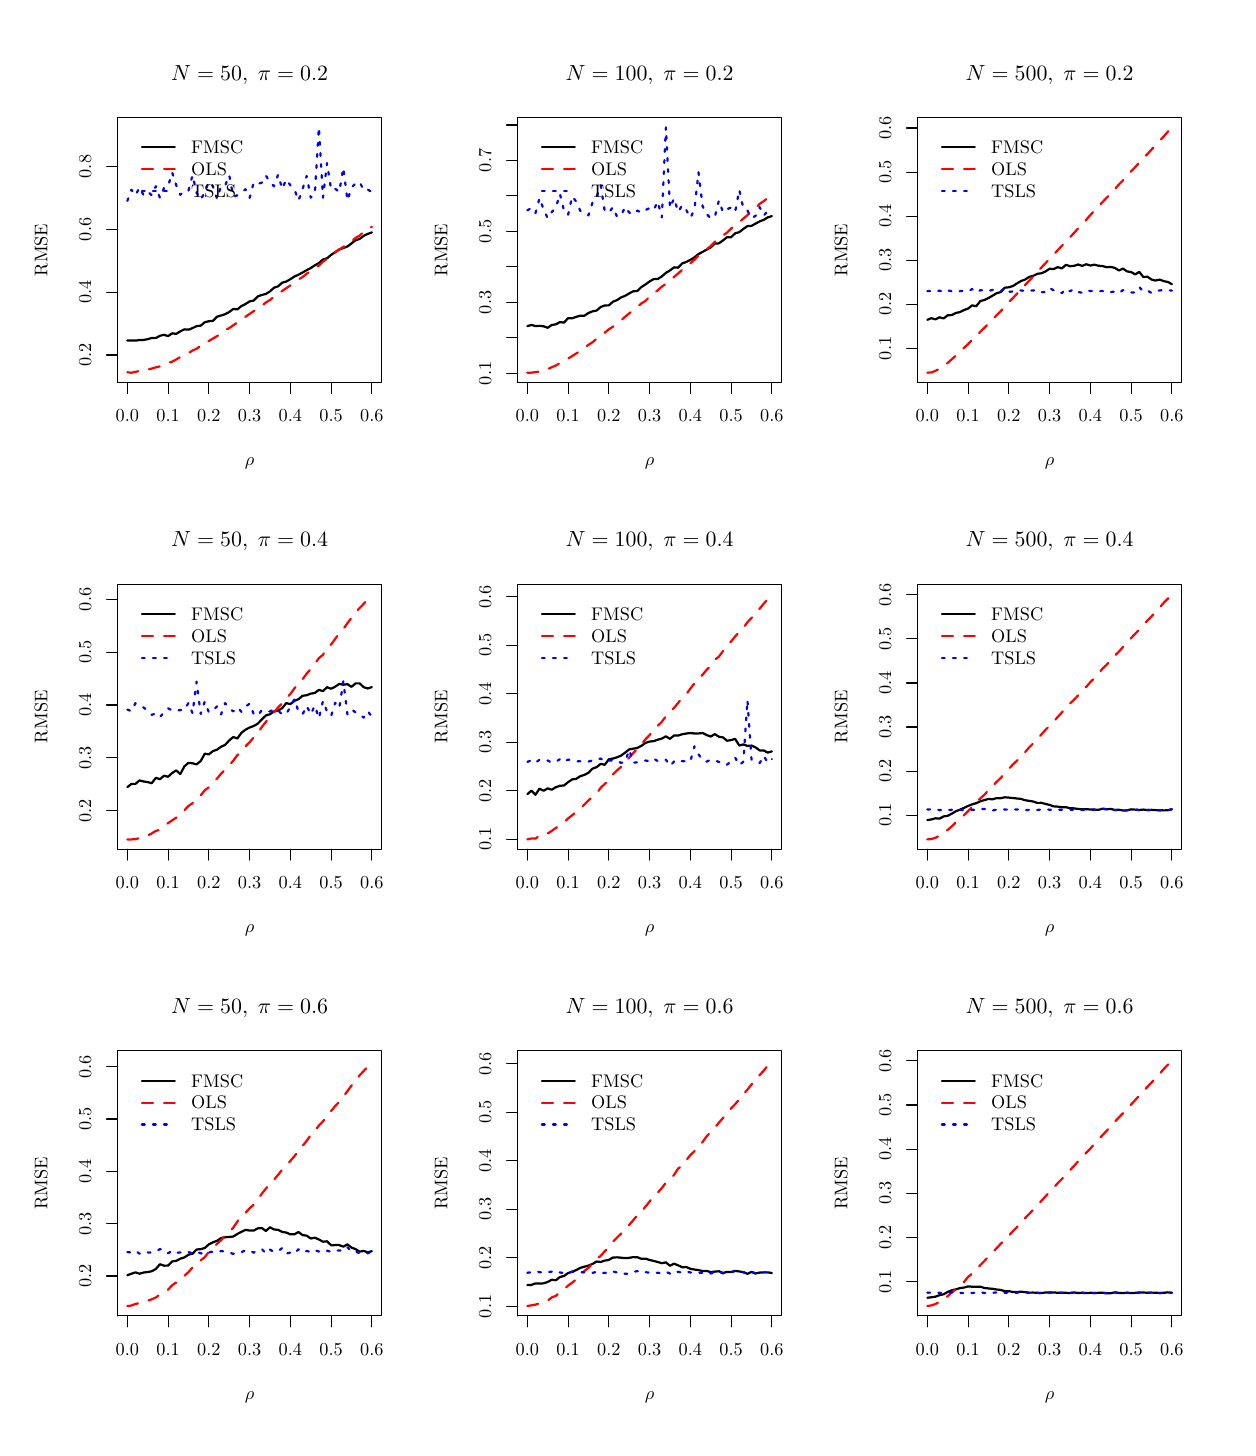
\begin{tikzpicture}[x=1pt,y=1pt]
\definecolor[named]{fillColor}{rgb}{1.00,1.00,1.00}
\path[use as bounding box,fill=fillColor,fill opacity=0.00] (0,0) rectangle (433.62,505.89);
\begin{scope}
\path[clip] ( 32.47,377.65) rectangle (127.91,473.42);
\definecolor[named]{drawColor}{rgb}{0.00,0.00,0.00}

\path[draw=drawColor,line width= 0.8pt,line join=round,line cap=round] ( 36.01,392.85) --
	( 37.48,392.85) --
	( 38.95,392.82) --
	( 40.42,392.99) --
	( 41.90,393.05) --
	( 43.37,393.32) --
	( 44.84,393.76) --
	( 46.32,393.73) --
	( 47.79,394.55) --
	( 49.26,394.91) --
	( 50.73,394.44) --
	( 52.21,395.44) --
	( 53.68,395.23) --
	( 55.15,396.16) --
	( 56.63,396.88) --
	( 58.10,396.76) --
	( 59.57,397.32) --
	( 61.04,398.05) --
	( 62.52,398.20) --
	( 63.99,399.44) --
	( 65.46,399.81) --
	( 66.93,399.94) --
	( 68.41,401.44) --
	( 69.88,401.88) --
	( 71.35,402.35) --
	( 72.83,403.14) --
	( 74.30,404.25) --
	( 75.77,404.09) --
	( 77.24,405.29) --
	( 78.72,406.02) --
	( 80.19,406.97) --
	( 81.66,407.27) --
	( 83.14,408.76) --
	( 84.61,409.31) --
	( 86.08,409.66) --
	( 87.55,410.59) --
	( 89.03,411.92) --
	( 90.50,412.42) --
	( 91.97,413.74) --
	( 93.44,414.14) --
	( 94.92,415.00) --
	( 96.39,415.97) --
	( 97.86,416.61) --
	( 99.34,417.42) --
	(100.81,418.25) --
	(102.28,419.03) --
	(103.75,420.01) --
	(105.23,420.82) --
	(106.70,422.09) --
	(108.17,422.54) --
	(109.65,423.80) --
	(111.12,424.77) --
	(112.59,425.70) --
	(114.06,426.28) --
	(115.54,426.81) --
	(117.01,427.93) --
	(118.48,429.07) --
	(119.95,429.54) --
	(121.43,430.66) --
	(122.90,431.38) --
	(124.37,431.90);
\end{scope}
\begin{scope}
\path[clip] (  0.00,  0.00) rectangle (433.62,505.89);
\definecolor[named]{drawColor}{rgb}{0.00,0.00,0.00}

\path[draw=drawColor,line width= 0.4pt,line join=round,line cap=round] ( 36.01,377.65) -- (124.37,377.65);

\path[draw=drawColor,line width= 0.4pt,line join=round,line cap=round] ( 36.01,377.65) -- ( 36.01,373.69);

\path[draw=drawColor,line width= 0.4pt,line join=round,line cap=round] ( 50.73,377.65) -- ( 50.73,373.69);

\path[draw=drawColor,line width= 0.4pt,line join=round,line cap=round] ( 65.46,377.65) -- ( 65.46,373.69);

\path[draw=drawColor,line width= 0.4pt,line join=round,line cap=round] ( 80.19,377.65) -- ( 80.19,373.69);

\path[draw=drawColor,line width= 0.4pt,line join=round,line cap=round] ( 94.92,377.65) -- ( 94.92,373.69);

\path[draw=drawColor,line width= 0.4pt,line join=round,line cap=round] (109.65,377.65) -- (109.65,373.69);

\path[draw=drawColor,line width= 0.4pt,line join=round,line cap=round] (124.37,377.65) -- (124.37,373.69);

\node[text=drawColor,anchor=base,inner sep=0pt, outer sep=0pt, scale=  0.66] at ( 36.01,363.40) {0.0};

\node[text=drawColor,anchor=base,inner sep=0pt, outer sep=0pt, scale=  0.66] at ( 50.73,363.40) {0.1};

\node[text=drawColor,anchor=base,inner sep=0pt, outer sep=0pt, scale=  0.66] at ( 65.46,363.40) {0.2};

\node[text=drawColor,anchor=base,inner sep=0pt, outer sep=0pt, scale=  0.66] at ( 80.19,363.40) {0.3};

\node[text=drawColor,anchor=base,inner sep=0pt, outer sep=0pt, scale=  0.66] at ( 94.92,363.40) {0.4};

\node[text=drawColor,anchor=base,inner sep=0pt, outer sep=0pt, scale=  0.66] at (109.65,363.40) {0.5};

\node[text=drawColor,anchor=base,inner sep=0pt, outer sep=0pt, scale=  0.66] at (124.37,363.40) {0.6};

\path[draw=drawColor,line width= 0.4pt,line join=round,line cap=round] ( 32.47,387.59) -- ( 32.47,455.73);

\path[draw=drawColor,line width= 0.4pt,line join=round,line cap=round] ( 32.47,387.59) -- ( 28.51,387.59);

\path[draw=drawColor,line width= 0.4pt,line join=round,line cap=round] ( 32.47,410.30) -- ( 28.51,410.30);

\path[draw=drawColor,line width= 0.4pt,line join=round,line cap=round] ( 32.47,433.02) -- ( 28.51,433.02);

\path[draw=drawColor,line width= 0.4pt,line join=round,line cap=round] ( 32.47,455.73) -- ( 28.51,455.73);

\node[text=drawColor,rotate= 90.00,anchor=base,inner sep=0pt, outer sep=0pt, scale=  0.66] at ( 22.97,387.59) {0.2};

\node[text=drawColor,rotate= 90.00,anchor=base,inner sep=0pt, outer sep=0pt, scale=  0.66] at ( 22.97,410.30) {0.4};

\node[text=drawColor,rotate= 90.00,anchor=base,inner sep=0pt, outer sep=0pt, scale=  0.66] at ( 22.97,433.02) {0.6};

\node[text=drawColor,rotate= 90.00,anchor=base,inner sep=0pt, outer sep=0pt, scale=  0.66] at ( 22.97,455.73) {0.8};

\path[draw=drawColor,line width= 0.4pt,line join=round,line cap=round] ( 32.47,377.65) --
	(127.91,377.65) --
	(127.91,473.42) --
	( 32.47,473.42) --
	( 32.47,377.65);
\end{scope}
\begin{scope}
\path[clip] (  0.00,337.26) rectangle (144.54,505.89);
\definecolor[named]{drawColor}{rgb}{0.00,0.00,0.00}

\node[text=drawColor,anchor=base,inner sep=0pt, outer sep=0pt, scale=  0.79] at ( 80.19,486.92) {\bfseries $N=50, \;\pi=0.2$};

\node[text=drawColor,anchor=base,inner sep=0pt, outer sep=0pt, scale=  0.66] at ( 80.19,347.56) {$\rho$};

\node[text=drawColor,rotate= 90.00,anchor=base,inner sep=0pt, outer sep=0pt, scale=  0.66] at (  7.13,425.53) {RMSE};
\end{scope}
\begin{scope}
\path[clip] ( 32.47,377.65) rectangle (127.91,473.42);
\definecolor[named]{drawColor}{rgb}{1.00,0.00,0.00}

\path[draw=drawColor,line width= 0.8pt,dash pattern=on 4pt off 4pt ,line join=round,line cap=round] ( 36.01,381.36) --
	( 37.48,381.20) --
	( 38.95,381.49) --
	( 40.42,381.86) --
	( 41.90,381.80) --
	( 43.37,382.32) --
	( 44.84,382.70) --
	( 46.32,383.15) --
	( 47.79,383.49) --
	( 49.26,384.27) --
	( 50.73,384.73) --
	( 52.21,385.20) --
	( 53.68,385.99) --
	( 55.15,386.88) --
	( 56.63,387.76) --
	( 58.10,388.30) --
	( 59.57,389.22) --
	( 61.04,389.85) --
	( 62.52,390.94) --
	( 63.99,392.08) --
	( 65.46,392.66) --
	( 66.93,393.54) --
	( 68.41,394.43) --
	( 69.88,395.21) --
	( 71.35,396.60) --
	( 72.83,397.31) --
	( 74.30,398.35) --
	( 75.77,399.35) --
	( 77.24,400.35) --
	( 78.72,401.43) --
	( 80.19,402.45) --
	( 81.66,403.45) --
	( 83.14,404.48) --
	( 84.61,405.41) --
	( 86.08,406.58) --
	( 87.55,407.49) --
	( 89.03,408.69) --
	( 90.50,409.35) --
	( 91.97,410.77) --
	( 93.44,411.75) --
	( 94.92,412.75) --
	( 96.39,414.06) --
	( 97.86,414.89) --
	( 99.34,415.77) --
	(100.81,416.98) --
	(102.28,417.93) --
	(103.75,419.08) --
	(105.23,419.91) --
	(106.70,421.31) --
	(108.17,422.34) --
	(109.65,423.54) --
	(111.12,424.75) --
	(112.59,425.76) --
	(114.06,426.67) --
	(115.54,427.66) --
	(117.01,428.70) --
	(118.48,429.92) --
	(119.95,430.74) --
	(121.43,432.08) --
	(122.90,433.23) --
	(124.37,433.92);
\definecolor[named]{drawColor}{rgb}{0.00,0.00,1.00}

\path[draw=drawColor,line width= 0.8pt,dash pattern=on 1pt off 3pt ,line join=round,line cap=round] ( 36.01,443.28) --
	( 37.48,447.36) --
	( 38.95,445.30) --
	( 40.42,448.16) --
	( 41.90,445.34) --
	( 43.37,446.58) --
	( 44.84,445.36) --
	( 46.32,448.60) --
	( 47.79,444.35) --
	( 49.26,447.89) --
	( 50.73,448.59) --
	( 52.21,453.56) --
	( 53.68,448.94) --
	( 55.15,445.48) --
	( 56.63,446.88) --
	( 58.10,446.98) --
	( 59.57,452.57) --
	( 61.04,446.27) --
	( 62.52,443.76) --
	( 63.99,446.35) --
	( 65.46,450.26) --
	( 66.93,448.68) --
	( 68.41,444.07) --
	( 69.88,448.63) --
	( 71.35,448.80) --
	( 72.83,452.57) --
	( 74.30,444.85) --
	( 75.77,445.31) --
	( 77.24,446.26) --
	( 78.72,447.50) --
	( 80.19,444.39) --
	( 81.66,449.87) --
	( 83.14,449.37) --
	( 84.61,449.91) --
	( 86.08,452.43) --
	( 87.55,450.07) --
	( 89.03,448.57) --
	( 90.50,452.79) --
	( 91.97,447.62) --
	( 93.44,451.06) --
	( 94.92,448.97) --
	( 96.39,447.49) --
	( 97.86,443.41) --
	( 99.34,447.60) --
	(100.81,452.30) --
	(102.28,444.47) --
	(103.75,445.83) --
	(105.23,469.87) --
	(106.70,444.43) --
	(108.17,456.95) --
	(109.65,447.37) --
	(111.12,447.67) --
	(112.59,446.52) --
	(114.06,455.25) --
	(115.54,443.48) --
	(117.01,448.03) --
	(118.48,449.65) --
	(119.95,450.13) --
	(121.43,447.14) --
	(122.90,447.40) --
	(124.37,446.42);
\definecolor[named]{drawColor}{rgb}{0.00,0.00,0.00}

\path[draw=drawColor,line width= 0.8pt,line join=round,line cap=round] ( 41.28,462.63) -- ( 53.16,462.63);
\definecolor[named]{drawColor}{rgb}{1.00,0.00,0.00}

\path[draw=drawColor,line width= 0.8pt,dash pattern=on 4pt off 4pt ,line join=round,line cap=round] ( 41.28,454.71) -- ( 53.16,454.71);
\definecolor[named]{drawColor}{rgb}{0.00,0.00,1.00}

\path[draw=drawColor,line width= 0.8pt,dash pattern=on 1pt off 3pt ,line join=round,line cap=round] ( 41.28,446.79) -- ( 53.16,446.79);
\definecolor[named]{drawColor}{rgb}{0.00,0.00,0.00}

\node[text=drawColor,anchor=base west,inner sep=0pt, outer sep=0pt, scale=  0.66] at ( 59.10,460.35) {FMSC};

\node[text=drawColor,anchor=base west,inner sep=0pt, outer sep=0pt, scale=  0.66] at ( 59.10,452.43) {OLS};

\node[text=drawColor,anchor=base west,inner sep=0pt, outer sep=0pt, scale=  0.66] at ( 59.10,444.51) {TSLS};
\end{scope}
\begin{scope}
\path[clip] (177.01,377.65) rectangle (272.45,473.42);
\definecolor[named]{drawColor}{rgb}{0.00,0.00,0.00}

\path[draw=drawColor,line width= 0.8pt,line join=round,line cap=round] (180.55,398.03) --
	(182.02,398.46) --
	(183.49,398.06) --
	(184.96,398.14) --
	(186.44,397.98) --
	(187.91,397.44) --
	(189.38,398.43) --
	(190.86,398.70) --
	(192.33,399.49) --
	(193.80,399.31) --
	(195.27,400.93) --
	(196.75,400.85) --
	(198.22,401.40) --
	(199.69,401.82) --
	(201.17,401.81) --
	(202.64,402.79) --
	(204.11,403.39) --
	(205.58,403.67) --
	(207.06,404.95) --
	(208.53,405.52) --
	(210.00,405.54) --
	(211.47,406.84) --
	(212.95,407.43) --
	(214.42,408.41) --
	(215.89,408.99) --
	(217.37,409.86) --
	(218.84,410.64) --
	(220.31,410.73) --
	(221.78,412.18) --
	(223.26,413.11) --
	(224.73,414.19) --
	(226.20,415.02) --
	(227.68,415.05) --
	(229.15,416.01) --
	(230.62,417.28) --
	(232.09,418.15) --
	(233.57,419.28) --
	(235.04,419.15) --
	(236.51,420.70) --
	(237.98,421.22) --
	(239.46,421.97) --
	(240.93,422.89) --
	(242.40,424.07) --
	(243.88,424.87) --
	(245.35,425.66) --
	(246.82,426.49) --
	(248.29,427.85) --
	(249.77,427.95) --
	(251.24,429.01) --
	(252.71,430.15) --
	(254.19,430.17) --
	(255.66,431.59) --
	(257.13,431.99) --
	(258.60,433.15) --
	(260.08,434.19) --
	(261.55,434.26) --
	(263.02,435.08) --
	(264.50,435.88) --
	(265.97,436.45) --
	(267.44,437.33) --
	(268.91,437.78);
\end{scope}
\begin{scope}
\path[clip] (  0.00,  0.00) rectangle (433.62,505.89);
\definecolor[named]{drawColor}{rgb}{0.00,0.00,0.00}

\path[draw=drawColor,line width= 0.4pt,line join=round,line cap=round] (180.55,377.65) -- (268.91,377.65);

\path[draw=drawColor,line width= 0.4pt,line join=round,line cap=round] (180.55,377.65) -- (180.55,373.69);

\path[draw=drawColor,line width= 0.4pt,line join=round,line cap=round] (195.27,377.65) -- (195.27,373.69);

\path[draw=drawColor,line width= 0.4pt,line join=round,line cap=round] (210.00,377.65) -- (210.00,373.69);

\path[draw=drawColor,line width= 0.4pt,line join=round,line cap=round] (224.73,377.65) -- (224.73,373.69);

\path[draw=drawColor,line width= 0.4pt,line join=round,line cap=round] (239.46,377.65) -- (239.46,373.69);

\path[draw=drawColor,line width= 0.4pt,line join=round,line cap=round] (254.19,377.65) -- (254.19,373.69);

\path[draw=drawColor,line width= 0.4pt,line join=round,line cap=round] (268.91,377.65) -- (268.91,373.69);

\node[text=drawColor,anchor=base,inner sep=0pt, outer sep=0pt, scale=  0.66] at (180.55,363.40) {0.0};

\node[text=drawColor,anchor=base,inner sep=0pt, outer sep=0pt, scale=  0.66] at (195.27,363.40) {0.1};

\node[text=drawColor,anchor=base,inner sep=0pt, outer sep=0pt, scale=  0.66] at (210.00,363.40) {0.2};

\node[text=drawColor,anchor=base,inner sep=0pt, outer sep=0pt, scale=  0.66] at (224.73,363.40) {0.3};

\node[text=drawColor,anchor=base,inner sep=0pt, outer sep=0pt, scale=  0.66] at (239.46,363.40) {0.4};

\node[text=drawColor,anchor=base,inner sep=0pt, outer sep=0pt, scale=  0.66] at (254.19,363.40) {0.5};

\node[text=drawColor,anchor=base,inner sep=0pt, outer sep=0pt, scale=  0.66] at (268.91,363.40) {0.6};

\path[draw=drawColor,line width= 0.4pt,line join=round,line cap=round] (177.01,380.98) -- (177.01,470.73);

\path[draw=drawColor,line width= 0.4pt,line join=round,line cap=round] (177.01,380.98) -- (173.05,380.98);

\path[draw=drawColor,line width= 0.4pt,line join=round,line cap=round] (177.01,393.81) -- (173.05,393.81);

\path[draw=drawColor,line width= 0.4pt,line join=round,line cap=round] (177.01,406.63) -- (173.05,406.63);

\path[draw=drawColor,line width= 0.4pt,line join=round,line cap=round] (177.01,419.45) -- (173.05,419.45);

\path[draw=drawColor,line width= 0.4pt,line join=round,line cap=round] (177.01,432.27) -- (173.05,432.27);

\path[draw=drawColor,line width= 0.4pt,line join=round,line cap=round] (177.01,445.09) -- (173.05,445.09);

\path[draw=drawColor,line width= 0.4pt,line join=round,line cap=round] (177.01,457.91) -- (173.05,457.91);

\path[draw=drawColor,line width= 0.4pt,line join=round,line cap=round] (177.01,470.73) -- (173.05,470.73);

\node[text=drawColor,rotate= 90.00,anchor=base,inner sep=0pt, outer sep=0pt, scale=  0.66] at (167.51,380.98) {0.1};

\node[text=drawColor,rotate= 90.00,anchor=base,inner sep=0pt, outer sep=0pt, scale=  0.66] at (167.51,406.63) {0.3};

\node[text=drawColor,rotate= 90.00,anchor=base,inner sep=0pt, outer sep=0pt, scale=  0.66] at (167.51,432.27) {0.5};

\node[text=drawColor,rotate= 90.00,anchor=base,inner sep=0pt, outer sep=0pt, scale=  0.66] at (167.51,457.91) {0.7};

\path[draw=drawColor,line width= 0.4pt,line join=round,line cap=round] (177.01,377.65) --
	(272.45,377.65) --
	(272.45,473.42) --
	(177.01,473.42) --
	(177.01,377.65);
\end{scope}
\begin{scope}
\path[clip] (144.54,337.26) rectangle (289.08,505.89);
\definecolor[named]{drawColor}{rgb}{0.00,0.00,0.00}

\node[text=drawColor,anchor=base,inner sep=0pt, outer sep=0pt, scale=  0.79] at (224.73,486.92) {\bfseries $N=100, \;\pi=0.2$};

\node[text=drawColor,anchor=base,inner sep=0pt, outer sep=0pt, scale=  0.66] at (224.73,347.56) {$\rho$};

\node[text=drawColor,rotate= 90.00,anchor=base,inner sep=0pt, outer sep=0pt, scale=  0.66] at (151.67,425.53) {RMSE};
\end{scope}
\begin{scope}
\path[clip] (177.01,377.65) rectangle (272.45,473.42);
\definecolor[named]{drawColor}{rgb}{1.00,0.00,0.00}

\path[draw=drawColor,line width= 0.8pt,dash pattern=on 4pt off 4pt ,line join=round,line cap=round] (180.55,381.20) --
	(182.02,381.23) --
	(183.49,381.43) --
	(184.96,381.60) --
	(186.44,382.23) --
	(187.91,382.50) --
	(189.38,383.19) --
	(190.86,383.79) --
	(192.33,384.67) --
	(193.80,385.59) --
	(195.27,386.31) --
	(196.75,387.22) --
	(198.22,388.17) --
	(199.69,389.13) --
	(201.17,390.25) --
	(202.64,391.29) --
	(204.11,392.22) --
	(205.58,393.47) --
	(207.06,394.73) --
	(208.53,395.67) --
	(210.00,396.91) --
	(211.47,397.81) --
	(212.95,398.99) --
	(214.42,400.12) --
	(215.89,401.44) --
	(217.37,402.65) --
	(218.84,403.80) --
	(220.31,404.91) --
	(221.78,406.26) --
	(223.26,407.17) --
	(224.73,408.69) --
	(226.20,409.91) --
	(227.68,410.98) --
	(229.15,412.30) --
	(230.62,413.35) --
	(232.09,414.48) --
	(233.57,415.81) --
	(235.04,417.05) --
	(236.51,418.43) --
	(237.98,419.47) --
	(239.46,420.74) --
	(240.93,422.00) --
	(242.40,423.55) --
	(243.88,424.51) --
	(245.35,425.79) --
	(246.82,426.96) --
	(248.29,428.47) --
	(249.77,429.76) --
	(251.24,430.77) --
	(252.71,431.84) --
	(254.19,433.27) --
	(255.66,434.50) --
	(257.13,435.65) --
	(258.60,436.89) --
	(260.08,438.13) --
	(261.55,439.44) --
	(263.02,440.65) --
	(264.50,442.23) --
	(265.97,443.19) --
	(267.44,444.40) --
	(268.91,445.81);
\definecolor[named]{drawColor}{rgb}{0.00,0.00,1.00}

\path[draw=drawColor,line width= 0.8pt,dash pattern=on 1pt off 3pt ,line join=round,line cap=round] (180.55,439.89) --
	(182.02,440.70) --
	(183.49,438.88) --
	(184.96,444.31) --
	(186.44,440.13) --
	(187.91,437.02) --
	(189.38,439.27) --
	(190.86,440.83) --
	(192.33,445.84) --
	(193.80,439.78) --
	(195.27,438.23) --
	(196.75,444.94) --
	(198.22,443.00) --
	(199.69,439.70) --
	(201.17,438.86) --
	(202.64,438.08) --
	(204.11,442.72) --
	(205.58,444.83) --
	(207.06,448.91) --
	(208.53,439.53) --
	(210.00,439.08) --
	(211.47,441.01) --
	(212.95,437.61) --
	(214.42,438.03) --
	(215.89,441.14) --
	(217.37,439.06) --
	(218.84,438.46) --
	(220.31,439.78) --
	(221.78,438.99) --
	(223.26,439.97) --
	(224.73,440.74) --
	(226.20,440.01) --
	(227.68,443.04) --
	(229.15,437.32) --
	(230.62,469.87) --
	(232.09,440.76) --
	(233.57,444.22) --
	(235.04,439.32) --
	(236.51,441.70) --
	(237.98,440.02) --
	(239.46,437.16) --
	(240.93,440.15) --
	(242.40,453.61) --
	(243.88,441.36) --
	(245.35,438.49) --
	(246.82,437.01) --
	(248.29,437.50) --
	(249.77,443.43) --
	(251.24,439.20) --
	(252.71,440.30) --
	(254.19,440.89) --
	(255.66,439.36) --
	(257.13,447.31) --
	(258.60,440.58) --
	(260.08,439.80) --
	(261.55,437.08) --
	(263.02,437.87) --
	(264.50,441.05) --
	(265.97,438.01) --
	(267.44,439.66) --
	(268.91,441.06);
\definecolor[named]{drawColor}{rgb}{0.00,0.00,0.00}

\path[draw=drawColor,line width= 0.8pt,line join=round,line cap=round] (185.82,462.63) -- (197.70,462.63);
\definecolor[named]{drawColor}{rgb}{1.00,0.00,0.00}

\path[draw=drawColor,line width= 0.8pt,dash pattern=on 4pt off 4pt ,line join=round,line cap=round] (185.82,454.71) -- (197.70,454.71);
\definecolor[named]{drawColor}{rgb}{0.00,0.00,1.00}

\path[draw=drawColor,line width= 0.8pt,dash pattern=on 1pt off 3pt ,line join=round,line cap=round] (185.82,446.79) -- (197.70,446.79);
\definecolor[named]{drawColor}{rgb}{0.00,0.00,0.00}

\node[text=drawColor,anchor=base west,inner sep=0pt, outer sep=0pt, scale=  0.66] at (203.64,460.35) {FMSC};

\node[text=drawColor,anchor=base west,inner sep=0pt, outer sep=0pt, scale=  0.66] at (203.64,452.43) {OLS};

\node[text=drawColor,anchor=base west,inner sep=0pt, outer sep=0pt, scale=  0.66] at (203.64,444.51) {TSLS};
\end{scope}
\begin{scope}
\path[clip] (321.55,377.65) rectangle (416.99,473.42);
\definecolor[named]{drawColor}{rgb}{0.00,0.00,0.00}

\path[draw=drawColor,line width= 0.8pt,line join=round,line cap=round] (325.09,400.32) --
	(326.56,400.91) --
	(328.03,400.48) --
	(329.50,401.23) --
	(330.98,400.82) --
	(332.45,401.95) --
	(333.92,402.04) --
	(335.40,402.79) --
	(336.87,403.13) --
	(338.34,403.85) --
	(339.81,404.38) --
	(341.29,405.54) --
	(342.76,405.24) --
	(344.23,407.08) --
	(345.71,407.50) --
	(347.18,408.19) --
	(348.65,409.05) --
	(350.12,409.93) --
	(351.60,410.34) --
	(353.07,411.93) --
	(354.54,412.07) --
	(356.01,412.52) --
	(357.49,413.48) --
	(358.96,414.34) --
	(360.43,414.88) --
	(361.91,415.84) --
	(363.38,416.21) --
	(364.85,416.94) --
	(366.32,417.15) --
	(367.80,417.79) --
	(369.27,418.77) --
	(370.74,418.66) --
	(372.22,419.36) --
	(373.69,418.90) --
	(375.16,420.17) --
	(376.63,419.69) --
	(378.11,419.81) --
	(379.58,420.31) --
	(381.05,419.81) --
	(382.52,420.39) --
	(384.00,419.94) --
	(385.47,420.24) --
	(386.94,419.86) --
	(388.42,419.73) --
	(389.89,419.34) --
	(391.36,419.41) --
	(392.83,419.09) --
	(394.31,418.14) --
	(395.78,418.82) --
	(397.25,417.82) --
	(398.73,417.57) --
	(400.20,416.75) --
	(401.67,417.63) --
	(403.14,415.78) --
	(404.62,415.89) --
	(406.09,414.88) --
	(407.56,414.51) --
	(409.04,414.86) --
	(410.51,414.30) --
	(411.98,414.00) --
	(413.45,413.21);
\end{scope}
\begin{scope}
\path[clip] (  0.00,  0.00) rectangle (433.62,505.89);
\definecolor[named]{drawColor}{rgb}{0.00,0.00,0.00}

\path[draw=drawColor,line width= 0.4pt,line join=round,line cap=round] (325.09,377.65) -- (413.45,377.65);

\path[draw=drawColor,line width= 0.4pt,line join=round,line cap=round] (325.09,377.65) -- (325.09,373.69);

\path[draw=drawColor,line width= 0.4pt,line join=round,line cap=round] (339.81,377.65) -- (339.81,373.69);

\path[draw=drawColor,line width= 0.4pt,line join=round,line cap=round] (354.54,377.65) -- (354.54,373.69);

\path[draw=drawColor,line width= 0.4pt,line join=round,line cap=round] (369.27,377.65) -- (369.27,373.69);

\path[draw=drawColor,line width= 0.4pt,line join=round,line cap=round] (384.00,377.65) -- (384.00,373.69);

\path[draw=drawColor,line width= 0.4pt,line join=round,line cap=round] (398.73,377.65) -- (398.73,373.69);

\path[draw=drawColor,line width= 0.4pt,line join=round,line cap=round] (413.45,377.65) -- (413.45,373.69);

\node[text=drawColor,anchor=base,inner sep=0pt, outer sep=0pt, scale=  0.66] at (325.09,363.40) {0.0};

\node[text=drawColor,anchor=base,inner sep=0pt, outer sep=0pt, scale=  0.66] at (339.81,363.40) {0.1};

\node[text=drawColor,anchor=base,inner sep=0pt, outer sep=0pt, scale=  0.66] at (354.54,363.40) {0.2};

\node[text=drawColor,anchor=base,inner sep=0pt, outer sep=0pt, scale=  0.66] at (369.27,363.40) {0.3};

\node[text=drawColor,anchor=base,inner sep=0pt, outer sep=0pt, scale=  0.66] at (384.00,363.40) {0.4};

\node[text=drawColor,anchor=base,inner sep=0pt, outer sep=0pt, scale=  0.66] at (398.73,363.40) {0.5};

\node[text=drawColor,anchor=base,inner sep=0pt, outer sep=0pt, scale=  0.66] at (413.45,363.40) {0.6};

\path[draw=drawColor,line width= 0.4pt,line join=round,line cap=round] (321.55,389.99) -- (321.55,469.62);

\path[draw=drawColor,line width= 0.4pt,line join=round,line cap=round] (321.55,389.99) -- (317.59,389.99);

\path[draw=drawColor,line width= 0.4pt,line join=round,line cap=round] (321.55,405.92) -- (317.59,405.92);

\path[draw=drawColor,line width= 0.4pt,line join=round,line cap=round] (321.55,421.84) -- (317.59,421.84);

\path[draw=drawColor,line width= 0.4pt,line join=round,line cap=round] (321.55,437.77) -- (317.59,437.77);

\path[draw=drawColor,line width= 0.4pt,line join=round,line cap=round] (321.55,453.69) -- (317.59,453.69);

\path[draw=drawColor,line width= 0.4pt,line join=round,line cap=round] (321.55,469.62) -- (317.59,469.62);

\node[text=drawColor,rotate= 90.00,anchor=base,inner sep=0pt, outer sep=0pt, scale=  0.66] at (312.05,389.99) {0.1};

\node[text=drawColor,rotate= 90.00,anchor=base,inner sep=0pt, outer sep=0pt, scale=  0.66] at (312.05,405.92) {0.2};

\node[text=drawColor,rotate= 90.00,anchor=base,inner sep=0pt, outer sep=0pt, scale=  0.66] at (312.05,421.84) {0.3};

\node[text=drawColor,rotate= 90.00,anchor=base,inner sep=0pt, outer sep=0pt, scale=  0.66] at (312.05,437.77) {0.4};

\node[text=drawColor,rotate= 90.00,anchor=base,inner sep=0pt, outer sep=0pt, scale=  0.66] at (312.05,453.69) {0.5};

\node[text=drawColor,rotate= 90.00,anchor=base,inner sep=0pt, outer sep=0pt, scale=  0.66] at (312.05,469.62) {0.6};

\path[draw=drawColor,line width= 0.4pt,line join=round,line cap=round] (321.55,377.65) --
	(416.99,377.65) --
	(416.99,473.42) --
	(321.55,473.42) --
	(321.55,377.65);
\end{scope}
\begin{scope}
\path[clip] (289.08,337.26) rectangle (433.62,505.89);
\definecolor[named]{drawColor}{rgb}{0.00,0.00,0.00}

\node[text=drawColor,anchor=base,inner sep=0pt, outer sep=0pt, scale=  0.79] at (369.27,486.92) {\bfseries $N=500, \;\pi=0.2$};

\node[text=drawColor,anchor=base,inner sep=0pt, outer sep=0pt, scale=  0.66] at (369.27,347.56) {$\rho$};

\node[text=drawColor,rotate= 90.00,anchor=base,inner sep=0pt, outer sep=0pt, scale=  0.66] at (296.21,425.53) {RMSE};
\end{scope}
\begin{scope}
\path[clip] (321.55,377.65) rectangle (416.99,473.42);
\definecolor[named]{drawColor}{rgb}{1.00,0.00,0.00}

\path[draw=drawColor,line width= 0.8pt,dash pattern=on 4pt off 4pt ,line join=round,line cap=round] (325.09,381.20) --
	(326.56,381.32) --
	(328.03,381.88) --
	(329.50,382.60) --
	(330.98,383.66) --
	(332.45,384.74) --
	(333.92,386.04) --
	(335.40,387.39) --
	(336.87,388.72) --
	(338.34,390.20) --
	(339.81,391.50) --
	(341.29,393.13) --
	(342.76,394.39) --
	(344.23,395.98) --
	(345.71,397.43) --
	(347.18,398.91) --
	(348.65,400.51) --
	(350.12,401.97) --
	(351.60,403.46) --
	(353.07,405.09) --
	(354.54,406.74) --
	(356.01,408.17) --
	(357.49,409.76) --
	(358.96,411.42) --
	(360.43,412.92) --
	(361.91,414.48) --
	(363.38,416.01) --
	(364.85,417.61) --
	(366.32,419.23) --
	(367.80,420.81) --
	(369.27,422.33) --
	(370.74,423.89) --
	(372.22,425.49) --
	(373.69,427.07) --
	(375.16,428.64) --
	(376.63,430.12) --
	(378.11,431.74) --
	(379.58,433.37) --
	(381.05,434.98) --
	(382.52,436.48) --
	(384.00,438.20) --
	(385.47,439.75) --
	(386.94,441.32) --
	(388.42,442.88) --
	(389.89,444.45) --
	(391.36,445.93) --
	(392.83,447.58) --
	(394.31,449.20) --
	(395.78,450.71) --
	(397.25,452.45) --
	(398.73,453.99) --
	(400.20,455.46) --
	(401.67,457.17) --
	(403.14,458.68) --
	(404.62,460.21) --
	(406.09,461.83) --
	(407.56,463.43) --
	(409.04,465.02) --
	(410.51,466.57) --
	(411.98,468.27) --
	(413.45,469.87);
\definecolor[named]{drawColor}{rgb}{0.00,0.00,1.00}

\path[draw=drawColor,line width= 0.8pt,dash pattern=on 1pt off 3pt ,line join=round,line cap=round] (325.09,410.68) --
	(326.56,410.73) --
	(328.03,410.53) --
	(329.50,410.86) --
	(330.98,410.35) --
	(332.45,410.97) --
	(333.92,410.62) --
	(335.40,410.83) --
	(336.87,410.67) --
	(338.34,410.84) --
	(339.81,410.62) --
	(341.29,411.42) --
	(342.76,410.19) --
	(344.23,411.01) --
	(345.71,411.03) --
	(347.18,410.73) --
	(348.65,411.14) --
	(350.12,411.01) --
	(351.60,410.63) --
	(353.07,411.81) --
	(354.54,410.46) --
	(356.01,410.54) --
	(357.49,410.98) --
	(358.96,410.95) --
	(360.43,410.70) --
	(361.91,410.85) --
	(363.38,410.93) --
	(364.85,411.12) --
	(366.32,410.29) --
	(367.80,410.38) --
	(369.27,411.78) --
	(370.74,410.97) --
	(372.22,410.87) --
	(373.69,409.95) --
	(375.16,411.62) --
	(376.63,410.63) --
	(378.11,411.43) --
	(379.58,410.37) --
	(381.05,410.09) --
	(382.52,410.92) --
	(384.00,410.73) --
	(385.47,410.78) --
	(386.94,410.62) --
	(388.42,410.76) --
	(389.89,410.21) --
	(391.36,410.37) --
	(392.83,410.50) --
	(394.31,409.92) --
	(395.78,411.05) --
	(397.25,410.83) --
	(398.73,410.22) --
	(400.20,410.18) --
	(401.67,412.12) --
	(403.14,410.57) --
	(404.62,410.92) --
	(406.09,410.02) --
	(407.56,410.69) --
	(409.04,410.93) --
	(410.51,411.07) --
	(411.98,411.06) --
	(413.45,410.87);
\definecolor[named]{drawColor}{rgb}{0.00,0.00,0.00}

\path[draw=drawColor,line width= 0.8pt,line join=round,line cap=round] (330.36,462.63) -- (342.24,462.63);
\definecolor[named]{drawColor}{rgb}{1.00,0.00,0.00}

\path[draw=drawColor,line width= 0.8pt,dash pattern=on 4pt off 4pt ,line join=round,line cap=round] (330.36,454.71) -- (342.24,454.71);
\definecolor[named]{drawColor}{rgb}{0.00,0.00,1.00}

\path[draw=drawColor,line width= 0.8pt,dash pattern=on 1pt off 3pt ,line join=round,line cap=round] (330.36,446.79) -- (342.24,446.79);
\definecolor[named]{drawColor}{rgb}{0.00,0.00,0.00}

\node[text=drawColor,anchor=base west,inner sep=0pt, outer sep=0pt, scale=  0.66] at (348.18,460.35) {FMSC};

\node[text=drawColor,anchor=base west,inner sep=0pt, outer sep=0pt, scale=  0.66] at (348.18,452.43) {OLS};

\node[text=drawColor,anchor=base west,inner sep=0pt, outer sep=0pt, scale=  0.66] at (348.18,444.51) {TSLS};
\end{scope}
\begin{scope}
\path[clip] ( 32.47,209.02) rectangle (127.91,304.79);
\definecolor[named]{drawColor}{rgb}{0.00,0.00,0.00}

\path[draw=drawColor,line width= 0.8pt,line join=round,line cap=round] ( 36.01,231.45) --
	( 37.48,232.62) --
	( 38.95,232.64) --
	( 40.42,233.88) --
	( 41.90,233.50) --
	( 43.37,233.27) --
	( 44.84,232.88) --
	( 46.32,234.83) --
	( 47.79,234.32) --
	( 49.26,235.57) --
	( 50.73,235.20) --
	( 52.21,236.56) --
	( 53.68,237.51) --
	( 55.15,236.18) --
	( 56.63,238.97) --
	( 58.10,240.23) --
	( 59.57,240.07) --
	( 61.04,239.68) --
	( 62.52,240.86) --
	( 63.99,243.54) --
	( 65.46,243.30) --
	( 66.93,244.48) --
	( 68.41,244.99) --
	( 69.88,246.05) --
	( 71.35,246.72) --
	( 72.83,248.34) --
	( 74.30,249.56) --
	( 75.77,249.04) --
	( 77.24,251.08) --
	( 78.72,252.21) --
	( 80.19,253.00) --
	( 81.66,253.54) --
	( 83.14,254.40) --
	( 84.61,255.93) --
	( 86.08,257.36) --
	( 87.55,257.80) --
	( 89.03,258.84) --
	( 90.50,259.14) --
	( 91.97,259.98) --
	( 93.44,261.84) --
	( 94.92,261.43) --
	( 96.39,262.63) --
	( 97.86,263.25) --
	( 99.34,264.47) --
	(100.81,264.66) --
	(102.28,265.24) --
	(103.75,265.48) --
	(105.23,266.59) --
	(106.70,266.16) --
	(108.17,267.55) --
	(109.65,267.02) --
	(111.12,267.76) --
	(112.59,268.74) --
	(114.06,268.47) --
	(115.54,268.66) --
	(117.01,267.69) --
	(118.48,268.95) --
	(119.95,268.95) --
	(121.43,267.56) --
	(122.90,267.11) --
	(124.37,267.59);
\end{scope}
\begin{scope}
\path[clip] (  0.00,  0.00) rectangle (433.62,505.89);
\definecolor[named]{drawColor}{rgb}{0.00,0.00,0.00}

\path[draw=drawColor,line width= 0.4pt,line join=round,line cap=round] ( 36.01,209.02) -- (124.37,209.02);

\path[draw=drawColor,line width= 0.4pt,line join=round,line cap=round] ( 36.01,209.02) -- ( 36.01,205.06);

\path[draw=drawColor,line width= 0.4pt,line join=round,line cap=round] ( 50.73,209.02) -- ( 50.73,205.06);

\path[draw=drawColor,line width= 0.4pt,line join=round,line cap=round] ( 65.46,209.02) -- ( 65.46,205.06);

\path[draw=drawColor,line width= 0.4pt,line join=round,line cap=round] ( 80.19,209.02) -- ( 80.19,205.06);

\path[draw=drawColor,line width= 0.4pt,line join=round,line cap=round] ( 94.92,209.02) -- ( 94.92,205.06);

\path[draw=drawColor,line width= 0.4pt,line join=round,line cap=round] (109.65,209.02) -- (109.65,205.06);

\path[draw=drawColor,line width= 0.4pt,line join=round,line cap=round] (124.37,209.02) -- (124.37,205.06);

\node[text=drawColor,anchor=base,inner sep=0pt, outer sep=0pt, scale=  0.66] at ( 36.01,194.77) {0.0};

\node[text=drawColor,anchor=base,inner sep=0pt, outer sep=0pt, scale=  0.66] at ( 50.73,194.77) {0.1};

\node[text=drawColor,anchor=base,inner sep=0pt, outer sep=0pt, scale=  0.66] at ( 65.46,194.77) {0.2};

\node[text=drawColor,anchor=base,inner sep=0pt, outer sep=0pt, scale=  0.66] at ( 80.19,194.77) {0.3};

\node[text=drawColor,anchor=base,inner sep=0pt, outer sep=0pt, scale=  0.66] at ( 94.92,194.77) {0.4};

\node[text=drawColor,anchor=base,inner sep=0pt, outer sep=0pt, scale=  0.66] at (109.65,194.77) {0.5};

\node[text=drawColor,anchor=base,inner sep=0pt, outer sep=0pt, scale=  0.66] at (124.37,194.77) {0.6};

\path[draw=drawColor,line width= 0.4pt,line join=round,line cap=round] ( 32.47,222.99) -- ( 32.47,299.31);

\path[draw=drawColor,line width= 0.4pt,line join=round,line cap=round] ( 32.47,222.99) -- ( 28.51,222.99);

\path[draw=drawColor,line width= 0.4pt,line join=round,line cap=round] ( 32.47,242.07) -- ( 28.51,242.07);

\path[draw=drawColor,line width= 0.4pt,line join=round,line cap=round] ( 32.47,261.15) -- ( 28.51,261.15);

\path[draw=drawColor,line width= 0.4pt,line join=round,line cap=round] ( 32.47,280.23) -- ( 28.51,280.23);

\path[draw=drawColor,line width= 0.4pt,line join=round,line cap=round] ( 32.47,299.31) -- ( 28.51,299.31);

\node[text=drawColor,rotate= 90.00,anchor=base,inner sep=0pt, outer sep=0pt, scale=  0.66] at ( 22.97,222.99) {0.2};

\node[text=drawColor,rotate= 90.00,anchor=base,inner sep=0pt, outer sep=0pt, scale=  0.66] at ( 22.97,242.07) {0.3};

\node[text=drawColor,rotate= 90.00,anchor=base,inner sep=0pt, outer sep=0pt, scale=  0.66] at ( 22.97,261.15) {0.4};

\node[text=drawColor,rotate= 90.00,anchor=base,inner sep=0pt, outer sep=0pt, scale=  0.66] at ( 22.97,280.23) {0.5};

\node[text=drawColor,rotate= 90.00,anchor=base,inner sep=0pt, outer sep=0pt, scale=  0.66] at ( 22.97,299.31) {0.6};

\path[draw=drawColor,line width= 0.4pt,line join=round,line cap=round] ( 32.47,209.02) --
	(127.91,209.02) --
	(127.91,304.79) --
	( 32.47,304.79) --
	( 32.47,209.02);
\end{scope}
\begin{scope}
\path[clip] (  0.00,168.63) rectangle (144.54,337.26);
\definecolor[named]{drawColor}{rgb}{0.00,0.00,0.00}

\node[text=drawColor,anchor=base,inner sep=0pt, outer sep=0pt, scale=  0.79] at ( 80.19,318.29) {\bfseries $N=50, \;\pi=0.4$};

\node[text=drawColor,anchor=base,inner sep=0pt, outer sep=0pt, scale=  0.66] at ( 80.19,178.93) {$\rho$};

\node[text=drawColor,rotate= 90.00,anchor=base,inner sep=0pt, outer sep=0pt, scale=  0.66] at (  7.13,256.90) {RMSE};
\end{scope}
\begin{scope}
\path[clip] ( 32.47,209.02) rectangle (127.91,304.79);
\definecolor[named]{drawColor}{rgb}{1.00,0.00,0.00}

\path[draw=drawColor,line width= 0.8pt,dash pattern=on 4pt off 4pt ,line join=round,line cap=round] ( 36.01,212.57) --
	( 37.48,212.57) --
	( 38.95,212.66) --
	( 40.42,213.06) --
	( 41.90,213.25) --
	( 43.37,213.95) --
	( 44.84,214.74) --
	( 46.32,215.64) --
	( 47.79,216.04) --
	( 49.26,217.31) --
	( 50.73,218.45) --
	( 52.21,219.44) --
	( 53.68,220.42) --
	( 55.15,221.39) --
	( 56.63,223.10) --
	( 58.10,224.64) --
	( 59.57,225.67) --
	( 61.04,226.93) --
	( 62.52,228.51) --
	( 63.99,230.28) --
	( 65.46,231.42) --
	( 66.93,233.17) --
	( 68.41,234.53) --
	( 69.88,236.32) --
	( 71.35,237.78) --
	( 72.83,239.36) --
	( 74.30,241.03) --
	( 75.77,243.02) --
	( 77.24,244.61) --
	( 78.72,246.24) --
	( 80.19,247.67) --
	( 81.66,249.43) --
	( 83.14,250.98) --
	( 84.61,253.17) --
	( 86.08,255.06) --
	( 87.55,256.58) --
	( 89.03,258.51) --
	( 90.50,260.26) --
	( 91.97,261.76) --
	( 93.44,263.60) --
	( 94.92,265.11) --
	( 96.39,267.16) --
	( 97.86,268.97) --
	( 99.34,270.44) --
	(100.81,272.45) --
	(102.28,274.13) --
	(103.75,275.99) --
	(105.23,278.07) --
	(106.70,279.26) --
	(108.17,281.94) --
	(109.65,283.01) --
	(111.12,285.02) --
	(112.59,287.13) --
	(114.06,288.58) --
	(115.54,290.70) --
	(117.01,292.61) --
	(118.48,294.70) --
	(119.95,296.20) --
	(121.43,297.69) --
	(122.90,299.35) --
	(124.37,301.24);
\definecolor[named]{drawColor}{rgb}{0.00,0.00,1.00}

\path[draw=drawColor,line width= 0.8pt,dash pattern=on 1pt off 3pt ,line join=round,line cap=round] ( 36.01,259.50) --
	( 37.48,258.88) --
	( 38.95,261.78) --
	( 40.42,260.84) --
	( 41.90,260.23) --
	( 43.37,259.03) --
	( 44.84,257.59) --
	( 46.32,258.06) --
	( 47.79,256.77) --
	( 49.26,258.44) --
	( 50.73,259.93) --
	( 52.21,259.14) --
	( 53.68,259.03) --
	( 55.15,259.32) --
	( 56.63,259.28) --
	( 58.10,261.89) --
	( 59.57,258.13) --
	( 61.04,269.58) --
	( 62.52,257.91) --
	( 63.99,262.34) --
	( 65.46,258.51) --
	( 66.93,259.13) --
	( 68.41,260.62) --
	( 69.88,257.75) --
	( 71.35,261.81) --
	( 72.83,259.87) --
	( 74.30,258.82) --
	( 75.77,260.31) --
	( 77.24,258.70) --
	( 78.72,260.54) --
	( 80.19,261.62) --
	( 81.66,257.90) --
	( 83.14,257.27) --
	( 84.61,259.28) --
	( 86.08,258.93) --
	( 87.55,258.81) --
	( 89.03,259.66) --
	( 90.50,259.20) --
	( 91.97,257.63) --
	( 93.44,257.98) --
	( 94.92,260.39) --
	( 96.39,263.29) --
	( 97.86,258.75) --
	( 99.34,257.79) --
	(100.81,260.84) --
	(102.28,257.75) --
	(103.75,260.92) --
	(105.23,256.33) --
	(106.70,262.62) --
	(108.17,258.76) --
	(109.65,257.16) --
	(111.12,261.95) --
	(112.59,260.01) --
	(114.06,269.68) --
	(115.54,257.75) --
	(117.01,259.58) --
	(118.48,258.43) --
	(119.95,257.70) --
	(121.43,256.58) --
	(122.90,258.91) --
	(124.37,256.88);
\definecolor[named]{drawColor}{rgb}{0.00,0.00,0.00}

\path[draw=drawColor,line width= 0.8pt,line join=round,line cap=round] ( 41.28,294.00) -- ( 53.16,294.00);
\definecolor[named]{drawColor}{rgb}{1.00,0.00,0.00}

\path[draw=drawColor,line width= 0.8pt,dash pattern=on 4pt off 4pt ,line join=round,line cap=round] ( 41.28,286.08) -- ( 53.16,286.08);
\definecolor[named]{drawColor}{rgb}{0.00,0.00,1.00}

\path[draw=drawColor,line width= 0.8pt,dash pattern=on 1pt off 3pt ,line join=round,line cap=round] ( 41.28,278.16) -- ( 53.16,278.16);
\definecolor[named]{drawColor}{rgb}{0.00,0.00,0.00}

\node[text=drawColor,anchor=base west,inner sep=0pt, outer sep=0pt, scale=  0.66] at ( 59.10,291.72) {FMSC};

\node[text=drawColor,anchor=base west,inner sep=0pt, outer sep=0pt, scale=  0.66] at ( 59.10,283.80) {OLS};

\node[text=drawColor,anchor=base west,inner sep=0pt, outer sep=0pt, scale=  0.66] at ( 59.10,275.88) {TSLS};
\end{scope}
\begin{scope}
\path[clip] (177.01,209.02) rectangle (272.45,304.79);
\definecolor[named]{drawColor}{rgb}{0.00,0.00,0.00}

\path[draw=drawColor,line width= 0.8pt,line join=round,line cap=round] (180.55,228.88) --
	(182.02,230.19) --
	(183.49,228.70) --
	(184.96,230.91) --
	(186.44,230.15) --
	(187.91,230.99) --
	(189.38,230.53) --
	(190.86,231.43) --
	(192.33,231.95) --
	(193.80,232.05) --
	(195.27,233.26) --
	(196.75,234.25) --
	(198.22,234.46) --
	(199.69,235.42) --
	(201.17,235.87) --
	(202.64,236.66) --
	(204.11,238.14) --
	(205.58,238.68) --
	(207.06,239.87) --
	(208.53,239.52) --
	(210.00,241.52) --
	(211.47,241.77) --
	(212.95,242.23) --
	(214.42,242.84) --
	(215.89,243.92) --
	(217.37,245.09) --
	(218.84,245.36) --
	(220.31,245.62) --
	(221.78,246.38) --
	(223.26,247.47) --
	(224.73,247.92) --
	(226.20,248.08) --
	(227.68,248.59) --
	(229.15,249.02) --
	(230.62,249.80) --
	(232.09,248.91) --
	(233.57,250.12) --
	(235.04,250.08) --
	(236.51,250.56) --
	(237.98,250.83) --
	(239.46,251.00) --
	(240.93,250.84) --
	(242.40,250.85) --
	(243.88,251.02) --
	(245.35,250.27) --
	(246.82,249.74) --
	(248.29,250.63) --
	(249.77,249.66) --
	(251.24,249.43) --
	(252.71,248.22) --
	(254.19,248.46) --
	(255.66,248.88) --
	(257.13,246.50) --
	(258.60,246.89) --
	(260.08,246.35) --
	(261.55,246.47) --
	(263.02,245.82) --
	(264.50,244.73) --
	(265.97,244.71) --
	(267.44,243.92) --
	(268.91,244.40);
\end{scope}
\begin{scope}
\path[clip] (  0.00,  0.00) rectangle (433.62,505.89);
\definecolor[named]{drawColor}{rgb}{0.00,0.00,0.00}

\path[draw=drawColor,line width= 0.4pt,line join=round,line cap=round] (180.55,209.02) -- (268.91,209.02);

\path[draw=drawColor,line width= 0.4pt,line join=round,line cap=round] (180.55,209.02) -- (180.55,205.06);

\path[draw=drawColor,line width= 0.4pt,line join=round,line cap=round] (195.27,209.02) -- (195.27,205.06);

\path[draw=drawColor,line width= 0.4pt,line join=round,line cap=round] (210.00,209.02) -- (210.00,205.06);

\path[draw=drawColor,line width= 0.4pt,line join=round,line cap=round] (224.73,209.02) -- (224.73,205.06);

\path[draw=drawColor,line width= 0.4pt,line join=round,line cap=round] (239.46,209.02) -- (239.46,205.06);

\path[draw=drawColor,line width= 0.4pt,line join=round,line cap=round] (254.19,209.02) -- (254.19,205.06);

\path[draw=drawColor,line width= 0.4pt,line join=round,line cap=round] (268.91,209.02) -- (268.91,205.06);

\node[text=drawColor,anchor=base,inner sep=0pt, outer sep=0pt, scale=  0.66] at (180.55,194.77) {0.0};

\node[text=drawColor,anchor=base,inner sep=0pt, outer sep=0pt, scale=  0.66] at (195.27,194.77) {0.1};

\node[text=drawColor,anchor=base,inner sep=0pt, outer sep=0pt, scale=  0.66] at (210.00,194.77) {0.2};

\node[text=drawColor,anchor=base,inner sep=0pt, outer sep=0pt, scale=  0.66] at (224.73,194.77) {0.3};

\node[text=drawColor,anchor=base,inner sep=0pt, outer sep=0pt, scale=  0.66] at (239.46,194.77) {0.4};

\node[text=drawColor,anchor=base,inner sep=0pt, outer sep=0pt, scale=  0.66] at (254.19,194.77) {0.5};

\node[text=drawColor,anchor=base,inner sep=0pt, outer sep=0pt, scale=  0.66] at (268.91,194.77) {0.6};

\path[draw=drawColor,line width= 0.4pt,line join=round,line cap=round] (177.01,212.60) -- (177.01,300.24);

\path[draw=drawColor,line width= 0.4pt,line join=round,line cap=round] (177.01,212.60) -- (173.05,212.60);

\path[draw=drawColor,line width= 0.4pt,line join=round,line cap=round] (177.01,230.13) -- (173.05,230.13);

\path[draw=drawColor,line width= 0.4pt,line join=round,line cap=round] (177.01,247.66) -- (173.05,247.66);

\path[draw=drawColor,line width= 0.4pt,line join=round,line cap=round] (177.01,265.18) -- (173.05,265.18);

\path[draw=drawColor,line width= 0.4pt,line join=round,line cap=round] (177.01,282.71) -- (173.05,282.71);

\path[draw=drawColor,line width= 0.4pt,line join=round,line cap=round] (177.01,300.24) -- (173.05,300.24);

\node[text=drawColor,rotate= 90.00,anchor=base,inner sep=0pt, outer sep=0pt, scale=  0.66] at (167.51,212.60) {0.1};

\node[text=drawColor,rotate= 90.00,anchor=base,inner sep=0pt, outer sep=0pt, scale=  0.66] at (167.51,230.13) {0.2};

\node[text=drawColor,rotate= 90.00,anchor=base,inner sep=0pt, outer sep=0pt, scale=  0.66] at (167.51,247.66) {0.3};

\node[text=drawColor,rotate= 90.00,anchor=base,inner sep=0pt, outer sep=0pt, scale=  0.66] at (167.51,265.18) {0.4};

\node[text=drawColor,rotate= 90.00,anchor=base,inner sep=0pt, outer sep=0pt, scale=  0.66] at (167.51,282.71) {0.5};

\node[text=drawColor,rotate= 90.00,anchor=base,inner sep=0pt, outer sep=0pt, scale=  0.66] at (167.51,300.24) {0.6};

\path[draw=drawColor,line width= 0.4pt,line join=round,line cap=round] (177.01,209.02) --
	(272.45,209.02) --
	(272.45,304.79) --
	(177.01,304.79) --
	(177.01,209.02);
\end{scope}
\begin{scope}
\path[clip] (144.54,168.63) rectangle (289.08,337.26);
\definecolor[named]{drawColor}{rgb}{0.00,0.00,0.00}

\node[text=drawColor,anchor=base,inner sep=0pt, outer sep=0pt, scale=  0.79] at (224.73,318.29) {\bfseries $N=100, \;\pi=0.4$};

\node[text=drawColor,anchor=base,inner sep=0pt, outer sep=0pt, scale=  0.66] at (224.73,178.93) {$\rho$};

\node[text=drawColor,rotate= 90.00,anchor=base,inner sep=0pt, outer sep=0pt, scale=  0.66] at (151.67,256.90) {RMSE};
\end{scope}
\begin{scope}
\path[clip] (177.01,209.02) rectangle (272.45,304.79);
\definecolor[named]{drawColor}{rgb}{1.00,0.00,0.00}

\path[draw=drawColor,line width= 0.8pt,dash pattern=on 4pt off 4pt ,line join=round,line cap=round] (180.55,212.57) --
	(182.02,212.91) --
	(183.49,212.84) --
	(184.96,213.88) --
	(186.44,213.90) --
	(187.91,214.72) --
	(189.38,215.65) --
	(190.86,216.73) --
	(192.33,217.50) --
	(193.80,218.72) --
	(195.27,220.14) --
	(196.75,221.27) --
	(198.22,222.58) --
	(199.69,223.74) --
	(201.17,225.19) --
	(202.64,226.67) --
	(204.11,227.96) --
	(205.58,229.16) --
	(207.06,231.23) --
	(208.53,232.63) --
	(210.00,233.78) --
	(211.47,236.02) --
	(212.95,237.51) --
	(214.42,238.78) --
	(215.89,240.70) --
	(217.37,242.12) --
	(218.84,243.79) --
	(220.31,245.37) --
	(221.78,246.96) --
	(223.26,248.78) --
	(224.73,250.27) --
	(226.20,251.98) --
	(227.68,253.64) --
	(229.15,255.07) --
	(230.62,257.06) --
	(232.09,258.63) --
	(233.57,260.12) --
	(235.04,261.88) --
	(236.51,263.74) --
	(237.98,265.02) --
	(239.46,267.07) --
	(240.93,268.95) --
	(242.40,270.23) --
	(243.88,272.11) --
	(245.35,273.85) --
	(246.82,275.35) --
	(248.29,277.44) --
	(249.77,278.61) --
	(251.24,280.59) --
	(252.71,282.39) --
	(254.19,284.09) --
	(255.66,285.94) --
	(257.13,287.46) --
	(258.60,288.95) --
	(260.08,291.02) --
	(261.55,292.61) --
	(263.02,294.15) --
	(264.50,295.97) --
	(265.97,297.75) --
	(267.44,299.40) --
	(268.91,301.24);
\definecolor[named]{drawColor}{rgb}{0.00,0.00,1.00}

\path[draw=drawColor,line width= 0.8pt,dash pattern=on 1pt off 3pt ,line join=round,line cap=round] (180.55,240.58) --
	(182.02,241.12) --
	(183.49,240.28) --
	(184.96,241.38) --
	(186.44,241.03) --
	(187.91,241.09) --
	(189.38,240.26) --
	(190.86,240.62) --
	(192.33,241.57) --
	(193.80,240.59) --
	(195.27,241.41) --
	(196.75,241.14) --
	(198.22,240.80) --
	(199.69,240.80) --
	(201.17,240.75) --
	(202.64,240.66) --
	(204.11,241.14) --
	(205.58,241.42) --
	(207.06,241.78) --
	(208.53,240.59) --
	(210.00,241.10) --
	(211.47,241.03) --
	(212.95,241.01) --
	(214.42,240.23) --
	(215.89,240.55) --
	(217.37,244.98) --
	(218.84,240.27) --
	(220.31,240.44) --
	(221.78,240.78) --
	(223.26,241.07) --
	(224.73,240.83) --
	(226.20,241.75) --
	(227.68,240.88) --
	(229.15,240.84) --
	(230.62,241.39) --
	(232.09,239.14) --
	(233.57,240.72) --
	(235.04,240.20) --
	(236.51,240.87) --
	(237.98,240.78) --
	(239.46,240.79) --
	(240.93,246.20) --
	(242.40,243.31) --
	(243.88,241.21) --
	(245.35,240.69) --
	(246.82,241.38) --
	(248.29,241.10) --
	(249.77,240.56) --
	(251.24,240.63) --
	(252.71,239.58) --
	(254.19,240.75) --
	(255.66,242.10) --
	(257.13,239.38) --
	(258.60,240.65) --
	(260.08,262.94) --
	(261.55,241.45) --
	(263.02,240.63) --
	(264.50,240.14) --
	(265.97,242.78) --
	(267.44,240.27) --
	(268.91,241.56);
\definecolor[named]{drawColor}{rgb}{0.00,0.00,0.00}

\path[draw=drawColor,line width= 0.8pt,line join=round,line cap=round] (185.82,294.00) -- (197.70,294.00);
\definecolor[named]{drawColor}{rgb}{1.00,0.00,0.00}

\path[draw=drawColor,line width= 0.8pt,dash pattern=on 4pt off 4pt ,line join=round,line cap=round] (185.82,286.08) -- (197.70,286.08);
\definecolor[named]{drawColor}{rgb}{0.00,0.00,1.00}

\path[draw=drawColor,line width= 0.8pt,dash pattern=on 1pt off 3pt ,line join=round,line cap=round] (185.82,278.16) -- (197.70,278.16);
\definecolor[named]{drawColor}{rgb}{0.00,0.00,0.00}

\node[text=drawColor,anchor=base west,inner sep=0pt, outer sep=0pt, scale=  0.66] at (203.64,291.72) {FMSC};

\node[text=drawColor,anchor=base west,inner sep=0pt, outer sep=0pt, scale=  0.66] at (203.64,283.80) {OLS};

\node[text=drawColor,anchor=base west,inner sep=0pt, outer sep=0pt, scale=  0.66] at (203.64,275.88) {TSLS};
\end{scope}
\begin{scope}
\path[clip] (321.55,209.02) rectangle (416.99,304.79);
\definecolor[named]{drawColor}{rgb}{0.00,0.00,0.00}

\path[draw=drawColor,line width= 0.8pt,line join=round,line cap=round] (325.09,219.55) --
	(326.56,219.79) --
	(328.03,220.20) --
	(329.50,220.07) --
	(330.98,220.88) --
	(332.45,221.10) --
	(333.92,221.85) --
	(335.40,222.75) --
	(336.87,223.30) --
	(338.34,223.96) --
	(339.81,224.65) --
	(341.29,225.24) --
	(342.76,225.66) --
	(344.23,226.32) --
	(345.71,226.78) --
	(347.18,227.20) --
	(348.65,227.05) --
	(350.12,227.49) --
	(351.60,227.45) --
	(353.07,227.78) --
	(354.54,227.67) --
	(356.01,227.52) --
	(357.49,227.35) --
	(358.96,227.20) --
	(360.43,226.73) --
	(361.91,226.49) --
	(363.38,226.25) --
	(364.85,225.76) --
	(366.32,225.78) --
	(367.80,225.38) --
	(369.27,225.03) --
	(370.74,224.51) --
	(372.22,224.40) --
	(373.69,224.16) --
	(375.16,224.20) --
	(376.63,223.85) --
	(378.11,223.78) --
	(379.58,223.58) --
	(381.05,223.42) --
	(382.52,223.49) --
	(384.00,223.37) --
	(385.47,223.36) --
	(386.94,223.23) --
	(388.42,223.69) --
	(389.89,223.44) --
	(391.36,223.60) --
	(392.83,223.19) --
	(394.31,223.29) --
	(395.78,223.02) --
	(397.25,223.07) --
	(398.73,223.43) --
	(400.20,223.32) --
	(401.67,223.19) --
	(403.14,223.34) --
	(404.62,223.15) --
	(406.09,223.25) --
	(407.56,223.15) --
	(409.04,223.12) --
	(410.51,223.05) --
	(411.98,223.09) --
	(413.45,223.48);
\end{scope}
\begin{scope}
\path[clip] (  0.00,  0.00) rectangle (433.62,505.89);
\definecolor[named]{drawColor}{rgb}{0.00,0.00,0.00}

\path[draw=drawColor,line width= 0.4pt,line join=round,line cap=round] (325.09,209.02) -- (413.45,209.02);

\path[draw=drawColor,line width= 0.4pt,line join=round,line cap=round] (325.09,209.02) -- (325.09,205.06);

\path[draw=drawColor,line width= 0.4pt,line join=round,line cap=round] (339.81,209.02) -- (339.81,205.06);

\path[draw=drawColor,line width= 0.4pt,line join=round,line cap=round] (354.54,209.02) -- (354.54,205.06);

\path[draw=drawColor,line width= 0.4pt,line join=round,line cap=round] (369.27,209.02) -- (369.27,205.06);

\path[draw=drawColor,line width= 0.4pt,line join=round,line cap=round] (384.00,209.02) -- (384.00,205.06);

\path[draw=drawColor,line width= 0.4pt,line join=round,line cap=round] (398.73,209.02) -- (398.73,205.06);

\path[draw=drawColor,line width= 0.4pt,line join=round,line cap=round] (413.45,209.02) -- (413.45,205.06);

\node[text=drawColor,anchor=base,inner sep=0pt, outer sep=0pt, scale=  0.66] at (325.09,194.77) {0.0};

\node[text=drawColor,anchor=base,inner sep=0pt, outer sep=0pt, scale=  0.66] at (339.81,194.77) {0.1};

\node[text=drawColor,anchor=base,inner sep=0pt, outer sep=0pt, scale=  0.66] at (354.54,194.77) {0.2};

\node[text=drawColor,anchor=base,inner sep=0pt, outer sep=0pt, scale=  0.66] at (369.27,194.77) {0.3};

\node[text=drawColor,anchor=base,inner sep=0pt, outer sep=0pt, scale=  0.66] at (384.00,194.77) {0.4};

\node[text=drawColor,anchor=base,inner sep=0pt, outer sep=0pt, scale=  0.66] at (398.73,194.77) {0.5};

\node[text=drawColor,anchor=base,inner sep=0pt, outer sep=0pt, scale=  0.66] at (413.45,194.77) {0.6};

\path[draw=drawColor,line width= 0.4pt,line join=round,line cap=round] (321.55,221.30) -- (321.55,300.96);

\path[draw=drawColor,line width= 0.4pt,line join=round,line cap=round] (321.55,221.30) -- (317.59,221.30);

\path[draw=drawColor,line width= 0.4pt,line join=round,line cap=round] (321.55,237.24) -- (317.59,237.24);

\path[draw=drawColor,line width= 0.4pt,line join=round,line cap=round] (321.55,253.17) -- (317.59,253.17);

\path[draw=drawColor,line width= 0.4pt,line join=round,line cap=round] (321.55,269.10) -- (317.59,269.10);

\path[draw=drawColor,line width= 0.4pt,line join=round,line cap=round] (321.55,285.03) -- (317.59,285.03);

\path[draw=drawColor,line width= 0.4pt,line join=round,line cap=round] (321.55,300.96) -- (317.59,300.96);

\node[text=drawColor,rotate= 90.00,anchor=base,inner sep=0pt, outer sep=0pt, scale=  0.66] at (312.05,221.30) {0.1};

\node[text=drawColor,rotate= 90.00,anchor=base,inner sep=0pt, outer sep=0pt, scale=  0.66] at (312.05,237.24) {0.2};

\node[text=drawColor,rotate= 90.00,anchor=base,inner sep=0pt, outer sep=0pt, scale=  0.66] at (312.05,253.17) {0.3};

\node[text=drawColor,rotate= 90.00,anchor=base,inner sep=0pt, outer sep=0pt, scale=  0.66] at (312.05,269.10) {0.4};

\node[text=drawColor,rotate= 90.00,anchor=base,inner sep=0pt, outer sep=0pt, scale=  0.66] at (312.05,285.03) {0.5};

\node[text=drawColor,rotate= 90.00,anchor=base,inner sep=0pt, outer sep=0pt, scale=  0.66] at (312.05,300.96) {0.6};

\path[draw=drawColor,line width= 0.4pt,line join=round,line cap=round] (321.55,209.02) --
	(416.99,209.02) --
	(416.99,304.79) --
	(321.55,304.79) --
	(321.55,209.02);
\end{scope}
\begin{scope}
\path[clip] (289.08,168.63) rectangle (433.62,337.26);
\definecolor[named]{drawColor}{rgb}{0.00,0.00,0.00}

\node[text=drawColor,anchor=base,inner sep=0pt, outer sep=0pt, scale=  0.79] at (369.27,318.29) {\bfseries $N=500, \;\pi=0.4$};

\node[text=drawColor,anchor=base,inner sep=0pt, outer sep=0pt, scale=  0.66] at (369.27,178.93) {$\rho$};

\node[text=drawColor,rotate= 90.00,anchor=base,inner sep=0pt, outer sep=0pt, scale=  0.66] at (296.21,256.90) {RMSE};
\end{scope}
\begin{scope}
\path[clip] (321.55,209.02) rectangle (416.99,304.79);
\definecolor[named]{drawColor}{rgb}{1.00,0.00,0.00}

\path[draw=drawColor,line width= 0.8pt,dash pattern=on 4pt off 4pt ,line join=round,line cap=round] (325.09,212.57) --
	(326.56,212.72) --
	(328.03,213.14) --
	(329.50,213.94) --
	(330.98,214.97) --
	(332.45,216.02) --
	(333.92,217.29) --
	(335.40,218.70) --
	(336.87,220.01) --
	(338.34,221.33) --
	(339.81,222.77) --
	(341.29,224.28) --
	(342.76,225.84) --
	(344.23,227.40) --
	(345.71,228.69) --
	(347.18,230.33) --
	(348.65,231.87) --
	(350.12,233.34) --
	(351.60,234.75) --
	(353.07,236.45) --
	(354.54,238.03) --
	(356.01,239.64) --
	(357.49,241.03) --
	(358.96,242.64) --
	(360.43,244.15) --
	(361.91,245.83) --
	(363.38,247.29) --
	(364.85,248.89) --
	(366.32,250.51) --
	(367.80,252.16) --
	(369.27,253.62) --
	(370.74,255.16) --
	(372.22,256.83) --
	(373.69,258.42) --
	(375.16,260.04) --
	(376.63,261.67) --
	(378.11,263.06) --
	(379.58,264.63) --
	(381.05,266.28) --
	(382.52,267.73) --
	(384.00,269.40) --
	(385.47,270.86) --
	(386.94,272.55) --
	(388.42,274.30) --
	(389.89,275.70) --
	(391.36,277.36) --
	(392.83,278.94) --
	(394.31,280.40) --
	(395.78,282.12) --
	(397.25,283.68) --
	(398.73,285.35) --
	(400.20,286.88) --
	(401.67,288.43) --
	(403.14,290.10) --
	(404.62,291.63) --
	(406.09,293.16) --
	(407.56,294.76) --
	(409.04,296.34) --
	(410.51,298.06) --
	(411.98,299.56) --
	(413.45,301.24);
\definecolor[named]{drawColor}{rgb}{0.00,0.00,1.00}

\path[draw=drawColor,line width= 0.8pt,dash pattern=on 1pt off 3pt ,line join=round,line cap=round] (325.09,223.39) --
	(326.56,223.43) --
	(328.03,223.50) --
	(329.50,223.13) --
	(330.98,223.36) --
	(332.45,223.18) --
	(333.92,223.26) --
	(335.40,223.45) --
	(336.87,223.26) --
	(338.34,223.21) --
	(339.81,223.37) --
	(341.29,223.28) --
	(342.76,223.19) --
	(344.23,223.55) --
	(345.71,223.55) --
	(347.18,223.52) --
	(348.65,223.02) --
	(350.12,223.30) --
	(351.60,223.34) --
	(353.07,223.37) --
	(354.54,223.28) --
	(356.01,223.36) --
	(357.49,223.40) --
	(358.96,223.35) --
	(360.43,223.11) --
	(361.91,223.25) --
	(363.38,223.31) --
	(364.85,223.22) --
	(366.32,223.35) --
	(367.80,223.48) --
	(369.27,223.29) --
	(370.74,223.21) --
	(372.22,223.27) --
	(373.69,223.29) --
	(375.16,223.32) --
	(376.63,223.32) --
	(378.11,223.32) --
	(379.58,223.30) --
	(381.05,223.19) --
	(382.52,223.35) --
	(384.00,223.27) --
	(385.47,223.25) --
	(386.94,223.20) --
	(388.42,223.64) --
	(389.89,223.40) --
	(391.36,223.58) --
	(392.83,223.18) --
	(394.31,223.28) --
	(395.78,223.02) --
	(397.25,223.07) --
	(398.73,223.43) --
	(400.20,223.32) --
	(401.67,223.19) --
	(403.14,223.34) --
	(404.62,223.15) --
	(406.09,223.25) --
	(407.56,223.15) --
	(409.04,223.12) --
	(410.51,223.05) --
	(411.98,223.09) --
	(413.45,223.48);
\definecolor[named]{drawColor}{rgb}{0.00,0.00,0.00}

\path[draw=drawColor,line width= 0.8pt,line join=round,line cap=round] (330.36,294.00) -- (342.24,294.00);
\definecolor[named]{drawColor}{rgb}{1.00,0.00,0.00}

\path[draw=drawColor,line width= 0.8pt,dash pattern=on 4pt off 4pt ,line join=round,line cap=round] (330.36,286.08) -- (342.24,286.08);
\definecolor[named]{drawColor}{rgb}{0.00,0.00,1.00}

\path[draw=drawColor,line width= 0.8pt,dash pattern=on 1pt off 3pt ,line join=round,line cap=round] (330.36,278.16) -- (342.24,278.16);
\definecolor[named]{drawColor}{rgb}{0.00,0.00,0.00}

\node[text=drawColor,anchor=base west,inner sep=0pt, outer sep=0pt, scale=  0.66] at (348.18,291.72) {FMSC};

\node[text=drawColor,anchor=base west,inner sep=0pt, outer sep=0pt, scale=  0.66] at (348.18,283.80) {OLS};

\node[text=drawColor,anchor=base west,inner sep=0pt, outer sep=0pt, scale=  0.66] at (348.18,275.88) {TSLS};
\end{scope}
\begin{scope}
\path[clip] ( 32.47, 40.39) rectangle (127.91,136.16);
\definecolor[named]{drawColor}{rgb}{0.00,0.00,0.00}

\path[draw=drawColor,line width= 0.8pt,line join=round,line cap=round] ( 36.01, 55.09) --
	( 37.48, 55.63) --
	( 38.95, 56.12) --
	( 40.42, 55.62) --
	( 41.90, 56.07) --
	( 43.37, 56.24) --
	( 44.84, 56.52) --
	( 46.32, 57.37) --
	( 47.79, 59.05) --
	( 49.26, 58.54) --
	( 50.73, 58.57) --
	( 52.21, 60.08) --
	( 53.68, 60.28) --
	( 55.15, 61.05) --
	( 56.63, 61.53) --
	( 58.10, 62.50) --
	( 59.57, 62.86) --
	( 61.04, 64.38) --
	( 62.52, 64.51) --
	( 63.99, 64.93) --
	( 65.46, 66.23) --
	( 66.93, 66.97) --
	( 68.41, 67.54) --
	( 69.88, 68.51) --
	( 71.35, 68.81) --
	( 72.83, 68.91) --
	( 74.30, 69.07) --
	( 75.77, 70.00) --
	( 77.24, 70.76) --
	( 78.72, 71.47) --
	( 80.19, 71.24) --
	( 81.66, 71.20) --
	( 83.14, 72.02) --
	( 84.61, 72.15) --
	( 86.08, 71.07) --
	( 87.55, 72.42) --
	( 89.03, 71.61) --
	( 90.50, 71.50) --
	( 91.97, 70.72) --
	( 93.44, 70.51) --
	( 94.92, 69.86) --
	( 96.39, 69.87) --
	( 97.86, 70.71) --
	( 99.34, 69.58) --
	(100.81, 69.39) --
	(102.28, 68.36) --
	(103.75, 68.64) --
	(105.23, 68.01) --
	(106.70, 67.19) --
	(108.17, 67.35) --
	(109.65, 65.91) --
	(111.12, 65.97) --
	(112.59, 65.98) --
	(114.06, 65.40) --
	(115.54, 66.25) --
	(117.01, 65.08) --
	(118.48, 64.52) --
	(119.95, 63.61) --
	(121.43, 63.86) --
	(122.90, 63.35) --
	(124.37, 63.78);
\end{scope}
\begin{scope}
\path[clip] (  0.00,  0.00) rectangle (433.62,505.89);
\definecolor[named]{drawColor}{rgb}{0.00,0.00,0.00}

\path[draw=drawColor,line width= 0.4pt,line join=round,line cap=round] ( 36.01, 40.39) -- (124.37, 40.39);

\path[draw=drawColor,line width= 0.4pt,line join=round,line cap=round] ( 36.01, 40.39) -- ( 36.01, 36.43);

\path[draw=drawColor,line width= 0.4pt,line join=round,line cap=round] ( 50.73, 40.39) -- ( 50.73, 36.43);

\path[draw=drawColor,line width= 0.4pt,line join=round,line cap=round] ( 65.46, 40.39) -- ( 65.46, 36.43);

\path[draw=drawColor,line width= 0.4pt,line join=round,line cap=round] ( 80.19, 40.39) -- ( 80.19, 36.43);

\path[draw=drawColor,line width= 0.4pt,line join=round,line cap=round] ( 94.92, 40.39) -- ( 94.92, 36.43);

\path[draw=drawColor,line width= 0.4pt,line join=round,line cap=round] (109.65, 40.39) -- (109.65, 36.43);

\path[draw=drawColor,line width= 0.4pt,line join=round,line cap=round] (124.37, 40.39) -- (124.37, 36.43);

\node[text=drawColor,anchor=base,inner sep=0pt, outer sep=0pt, scale=  0.66] at ( 36.01, 26.14) {0.0};

\node[text=drawColor,anchor=base,inner sep=0pt, outer sep=0pt, scale=  0.66] at ( 50.73, 26.14) {0.1};

\node[text=drawColor,anchor=base,inner sep=0pt, outer sep=0pt, scale=  0.66] at ( 65.46, 26.14) {0.2};

\node[text=drawColor,anchor=base,inner sep=0pt, outer sep=0pt, scale=  0.66] at ( 80.19, 26.14) {0.3};

\node[text=drawColor,anchor=base,inner sep=0pt, outer sep=0pt, scale=  0.66] at ( 94.92, 26.14) {0.4};

\node[text=drawColor,anchor=base,inner sep=0pt, outer sep=0pt, scale=  0.66] at (109.65, 26.14) {0.5};

\node[text=drawColor,anchor=base,inner sep=0pt, outer sep=0pt, scale=  0.66] at (124.37, 26.14) {0.6};

\path[draw=drawColor,line width= 0.4pt,line join=round,line cap=round] ( 32.47, 54.82) -- ( 32.47,130.42);

\path[draw=drawColor,line width= 0.4pt,line join=round,line cap=round] ( 32.47, 54.82) -- ( 28.51, 54.82);

\path[draw=drawColor,line width= 0.4pt,line join=round,line cap=round] ( 32.47, 73.72) -- ( 28.51, 73.72);

\path[draw=drawColor,line width= 0.4pt,line join=round,line cap=round] ( 32.47, 92.62) -- ( 28.51, 92.62);

\path[draw=drawColor,line width= 0.4pt,line join=round,line cap=round] ( 32.47,111.52) -- ( 28.51,111.52);

\path[draw=drawColor,line width= 0.4pt,line join=round,line cap=round] ( 32.47,130.42) -- ( 28.51,130.42);

\node[text=drawColor,rotate= 90.00,anchor=base,inner sep=0pt, outer sep=0pt, scale=  0.66] at ( 22.97, 54.82) {0.2};

\node[text=drawColor,rotate= 90.00,anchor=base,inner sep=0pt, outer sep=0pt, scale=  0.66] at ( 22.97, 73.72) {0.3};

\node[text=drawColor,rotate= 90.00,anchor=base,inner sep=0pt, outer sep=0pt, scale=  0.66] at ( 22.97, 92.62) {0.4};

\node[text=drawColor,rotate= 90.00,anchor=base,inner sep=0pt, outer sep=0pt, scale=  0.66] at ( 22.97,111.52) {0.5};

\node[text=drawColor,rotate= 90.00,anchor=base,inner sep=0pt, outer sep=0pt, scale=  0.66] at ( 22.97,130.42) {0.6};

\path[draw=drawColor,line width= 0.4pt,line join=round,line cap=round] ( 32.47, 40.39) --
	(127.91, 40.39) --
	(127.91,136.16) --
	( 32.47,136.16) --
	( 32.47, 40.39);
\end{scope}
\begin{scope}
\path[clip] (  0.00,  0.00) rectangle (144.54,168.63);
\definecolor[named]{drawColor}{rgb}{0.00,0.00,0.00}

\node[text=drawColor,anchor=base,inner sep=0pt, outer sep=0pt, scale=  0.79] at ( 80.19,149.66) {\bfseries $N=50, \;\pi=0.6$};

\node[text=drawColor,anchor=base,inner sep=0pt, outer sep=0pt, scale=  0.66] at ( 80.19, 10.30) {$\rho$};

\node[text=drawColor,rotate= 90.00,anchor=base,inner sep=0pt, outer sep=0pt, scale=  0.66] at (  7.13, 88.27) {RMSE};
\end{scope}
\begin{scope}
\path[clip] ( 32.47, 40.39) rectangle (127.91,136.16);
\definecolor[named]{drawColor}{rgb}{1.00,0.00,0.00}

\path[draw=drawColor,line width= 0.8pt,dash pattern=on 4pt off 4pt ,line join=round,line cap=round] ( 36.01, 43.94) --
	( 37.48, 44.13) --
	( 38.95, 44.71) --
	( 40.42, 45.01) --
	( 41.90, 45.31) --
	( 43.37, 45.89) --
	( 44.84, 46.38) --
	( 46.32, 47.05) --
	( 47.79, 48.13) --
	( 49.26, 48.76) --
	( 50.73, 49.86) --
	( 52.21, 51.47) --
	( 53.68, 52.46) --
	( 55.15, 53.20) --
	( 56.63, 54.86) --
	( 58.10, 56.20) --
	( 59.57, 57.88) --
	( 61.04, 59.26) --
	( 62.52, 60.46) --
	( 63.99, 61.60) --
	( 65.46, 63.49) --
	( 66.93, 64.58) --
	( 68.41, 66.45) --
	( 69.88, 67.72) --
	( 71.35, 69.49) --
	( 72.83, 70.71) --
	( 74.30, 72.28) --
	( 75.77, 74.46) --
	( 77.24, 76.54) --
	( 78.72, 77.61) --
	( 80.19, 79.28) --
	( 81.66, 80.57) --
	( 83.14, 82.51) --
	( 84.61, 84.55) --
	( 86.08, 86.36) --
	( 87.55, 88.29) --
	( 89.03, 89.64) --
	( 90.50, 91.35) --
	( 91.97, 93.28) --
	( 93.44, 94.54) --
	( 94.92, 96.40) --
	( 96.39, 98.10) --
	( 97.86,100.08) --
	( 99.34,101.84) --
	(100.81,103.64) --
	(102.28,105.72) --
	(103.75,107.19) --
	(105.23,109.17) --
	(106.70,110.68) --
	(108.17,112.48) --
	(109.65,114.44) --
	(111.12,116.21) --
	(112.59,117.74) --
	(114.06,119.61) --
	(115.54,121.62) --
	(117.01,123.59) --
	(118.48,125.09) --
	(119.95,127.34) --
	(121.43,128.87) --
	(122.90,130.52) --
	(124.37,132.61);
\definecolor[named]{drawColor}{rgb}{0.00,0.00,1.00}

\path[draw=drawColor,line width= 0.8pt,dash pattern=on 1pt off 3pt ,line join=round,line cap=round] ( 36.01, 63.44) --
	( 37.48, 63.33) --
	( 38.95, 63.94) --
	( 40.42, 62.85) --
	( 41.90, 63.52) --
	( 43.37, 63.35) --
	( 44.84, 63.25) --
	( 46.32, 63.71) --
	( 47.79, 64.52) --
	( 49.26, 64.17) --
	( 50.73, 63.03) --
	( 52.21, 63.91) --
	( 53.68, 63.14) --
	( 55.15, 63.34) --
	( 56.63, 63.20) --
	( 58.10, 63.49) --
	( 59.57, 62.91) --
	( 61.04, 63.51) --
	( 62.52, 63.03) --
	( 63.99, 62.69) --
	( 65.46, 63.31) --
	( 66.93, 63.61) --
	( 68.41, 63.43) --
	( 69.88, 63.83) --
	( 71.35, 63.57) --
	( 72.83, 63.32) --
	( 74.30, 62.80) --
	( 75.77, 63.24) --
	( 77.24, 63.40) --
	( 78.72, 64.13) --
	( 80.19, 63.95) --
	( 81.66, 63.26) --
	( 83.14, 64.08) --
	( 84.61, 64.53) --
	( 86.08, 62.94) --
	( 87.55, 64.35) --
	( 89.03, 63.47) --
	( 90.50, 63.79) --
	( 91.97, 64.91) --
	( 93.44, 62.89) --
	( 94.92, 63.28) --
	( 96.39, 62.89) --
	( 97.86, 64.47) --
	( 99.34, 63.36) --
	(100.81, 63.87) --
	(102.28, 63.42) --
	(103.75, 64.11) --
	(105.23, 63.67) --
	(106.70, 63.32) --
	(108.17, 63.95) --
	(109.65, 63.53) --
	(111.12, 63.95) --
	(112.59, 64.06) --
	(114.06, 63.82) --
	(115.54, 65.18) --
	(117.01, 63.68) --
	(118.48, 63.69) --
	(119.95, 63.01) --
	(121.43, 63.34) --
	(122.90, 63.02) --
	(124.37, 63.64);
\definecolor[named]{drawColor}{rgb}{0.00,0.00,0.00}

\path[draw=drawColor,line width= 0.8pt,line join=round,line cap=round] ( 41.28,125.37) -- ( 53.16,125.37);
\definecolor[named]{drawColor}{rgb}{1.00,0.00,0.00}

\path[draw=drawColor,line width= 0.8pt,dash pattern=on 4pt off 4pt ,line join=round,line cap=round] ( 41.28,117.45) -- ( 53.16,117.45);
\definecolor[named]{drawColor}{rgb}{0.00,0.00,1.00}

\path[draw=drawColor,line width= 0.8pt,dash pattern=on 1pt off 3pt ,line join=round,line cap=round] ( 41.28,109.53) -- ( 53.16,109.53);
\definecolor[named]{drawColor}{rgb}{0.00,0.00,0.00}

\node[text=drawColor,anchor=base west,inner sep=0pt, outer sep=0pt, scale=  0.66] at ( 59.10,123.09) {FMSC};

\node[text=drawColor,anchor=base west,inner sep=0pt, outer sep=0pt, scale=  0.66] at ( 59.10,115.17) {OLS};

\node[text=drawColor,anchor=base west,inner sep=0pt, outer sep=0pt, scale=  0.66] at ( 59.10,107.25) {TSLS};
\end{scope}
\begin{scope}
\path[clip] (177.01, 40.39) rectangle (272.45,136.16);
\definecolor[named]{drawColor}{rgb}{0.00,0.00,0.00}

\path[draw=drawColor,line width= 0.8pt,line join=round,line cap=round] (180.55, 51.53) --
	(182.02, 51.57) --
	(183.49, 52.13) --
	(184.96, 52.08) --
	(186.44, 52.15) --
	(187.91, 52.65) --
	(189.38, 53.46) --
	(190.86, 53.26) --
	(192.33, 54.44) --
	(193.80, 54.81) --
	(195.27, 55.86) --
	(196.75, 56.33) --
	(198.22, 56.95) --
	(199.69, 57.74) --
	(201.17, 58.17) --
	(202.64, 58.56) --
	(204.11, 59.17) --
	(205.58, 60.03) --
	(207.06, 59.88) --
	(208.53, 60.36) --
	(210.00, 60.63) --
	(211.47, 61.48) --
	(212.95, 61.55) --
	(214.42, 61.43) --
	(215.89, 61.26) --
	(217.37, 61.37) --
	(218.84, 61.63) --
	(220.31, 61.58) --
	(221.78, 61.02) --
	(223.26, 61.07) --
	(224.73, 60.60) --
	(226.20, 60.26) --
	(227.68, 59.85) --
	(229.15, 59.44) --
	(230.62, 59.73) --
	(232.09, 58.50) --
	(233.57, 59.26) --
	(235.04, 58.66) --
	(236.51, 57.96) --
	(237.98, 58.05) --
	(239.46, 57.41) --
	(240.93, 57.14) --
	(242.40, 56.94) --
	(243.88, 56.59) --
	(245.35, 56.66) --
	(246.82, 56.18) --
	(248.29, 56.40) --
	(249.77, 56.51) --
	(251.24, 55.91) --
	(252.71, 56.28) --
	(254.19, 56.23) --
	(255.66, 56.65) --
	(257.13, 56.45) --
	(258.60, 56.19) --
	(260.08, 55.60) --
	(261.55, 56.28) --
	(263.02, 55.72) --
	(264.50, 56.04) --
	(265.97, 56.12) --
	(267.44, 56.11) --
	(268.91, 55.88);
\end{scope}
\begin{scope}
\path[clip] (  0.00,  0.00) rectangle (433.62,505.89);
\definecolor[named]{drawColor}{rgb}{0.00,0.00,0.00}

\path[draw=drawColor,line width= 0.4pt,line join=round,line cap=round] (180.55, 40.39) -- (268.91, 40.39);

\path[draw=drawColor,line width= 0.4pt,line join=round,line cap=round] (180.55, 40.39) -- (180.55, 36.43);

\path[draw=drawColor,line width= 0.4pt,line join=round,line cap=round] (195.27, 40.39) -- (195.27, 36.43);

\path[draw=drawColor,line width= 0.4pt,line join=round,line cap=round] (210.00, 40.39) -- (210.00, 36.43);

\path[draw=drawColor,line width= 0.4pt,line join=round,line cap=round] (224.73, 40.39) -- (224.73, 36.43);

\path[draw=drawColor,line width= 0.4pt,line join=round,line cap=round] (239.46, 40.39) -- (239.46, 36.43);

\path[draw=drawColor,line width= 0.4pt,line join=round,line cap=round] (254.19, 40.39) -- (254.19, 36.43);

\path[draw=drawColor,line width= 0.4pt,line join=round,line cap=round] (268.91, 40.39) -- (268.91, 36.43);

\node[text=drawColor,anchor=base,inner sep=0pt, outer sep=0pt, scale=  0.66] at (180.55, 26.14) {0.0};

\node[text=drawColor,anchor=base,inner sep=0pt, outer sep=0pt, scale=  0.66] at (195.27, 26.14) {0.1};

\node[text=drawColor,anchor=base,inner sep=0pt, outer sep=0pt, scale=  0.66] at (210.00, 26.14) {0.2};

\node[text=drawColor,anchor=base,inner sep=0pt, outer sep=0pt, scale=  0.66] at (224.73, 26.14) {0.3};

\node[text=drawColor,anchor=base,inner sep=0pt, outer sep=0pt, scale=  0.66] at (239.46, 26.14) {0.4};

\node[text=drawColor,anchor=base,inner sep=0pt, outer sep=0pt, scale=  0.66] at (254.19, 26.14) {0.5};

\node[text=drawColor,anchor=base,inner sep=0pt, outer sep=0pt, scale=  0.66] at (268.91, 26.14) {0.6};

\path[draw=drawColor,line width= 0.4pt,line join=round,line cap=round] (177.01, 43.84) -- (177.01,131.50);

\path[draw=drawColor,line width= 0.4pt,line join=round,line cap=round] (177.01, 43.84) -- (173.05, 43.84);

\path[draw=drawColor,line width= 0.4pt,line join=round,line cap=round] (177.01, 61.38) -- (173.05, 61.38);

\path[draw=drawColor,line width= 0.4pt,line join=round,line cap=round] (177.01, 78.91) -- (173.05, 78.91);

\path[draw=drawColor,line width= 0.4pt,line join=round,line cap=round] (177.01, 96.44) -- (173.05, 96.44);

\path[draw=drawColor,line width= 0.4pt,line join=round,line cap=round] (177.01,113.97) -- (173.05,113.97);

\path[draw=drawColor,line width= 0.4pt,line join=round,line cap=round] (177.01,131.50) -- (173.05,131.50);

\node[text=drawColor,rotate= 90.00,anchor=base,inner sep=0pt, outer sep=0pt, scale=  0.66] at (167.51, 43.84) {0.1};

\node[text=drawColor,rotate= 90.00,anchor=base,inner sep=0pt, outer sep=0pt, scale=  0.66] at (167.51, 61.38) {0.2};

\node[text=drawColor,rotate= 90.00,anchor=base,inner sep=0pt, outer sep=0pt, scale=  0.66] at (167.51, 78.91) {0.3};

\node[text=drawColor,rotate= 90.00,anchor=base,inner sep=0pt, outer sep=0pt, scale=  0.66] at (167.51, 96.44) {0.4};

\node[text=drawColor,rotate= 90.00,anchor=base,inner sep=0pt, outer sep=0pt, scale=  0.66] at (167.51,113.97) {0.5};

\node[text=drawColor,rotate= 90.00,anchor=base,inner sep=0pt, outer sep=0pt, scale=  0.66] at (167.51,131.50) {0.6};

\path[draw=drawColor,line width= 0.4pt,line join=round,line cap=round] (177.01, 40.39) --
	(272.45, 40.39) --
	(272.45,136.16) --
	(177.01,136.16) --
	(177.01, 40.39);
\end{scope}
\begin{scope}
\path[clip] (144.54,  0.00) rectangle (289.08,168.63);
\definecolor[named]{drawColor}{rgb}{0.00,0.00,0.00}

\node[text=drawColor,anchor=base,inner sep=0pt, outer sep=0pt, scale=  0.79] at (224.73,149.66) {\bfseries $N=100, \;\pi=0.6$};

\node[text=drawColor,anchor=base,inner sep=0pt, outer sep=0pt, scale=  0.66] at (224.73, 10.30) {$\rho$};

\node[text=drawColor,rotate= 90.00,anchor=base,inner sep=0pt, outer sep=0pt, scale=  0.66] at (151.67, 88.27) {RMSE};
\end{scope}
\begin{scope}
\path[clip] (177.01, 40.39) rectangle (272.45,136.16);
\definecolor[named]{drawColor}{rgb}{1.00,0.00,0.00}

\path[draw=drawColor,line width= 0.8pt,dash pattern=on 4pt off 4pt ,line join=round,line cap=round] (180.55, 43.94) --
	(182.02, 44.21) --
	(183.49, 44.45) --
	(184.96, 44.92) --
	(186.44, 45.24) --
	(187.91, 45.87) --
	(189.38, 47.07) --
	(190.86, 47.63) --
	(192.33, 49.00) --
	(193.80, 49.95) --
	(195.27, 51.35) --
	(196.75, 52.40) --
	(198.22, 53.56) --
	(199.69, 55.07) --
	(201.17, 56.63) --
	(202.64, 57.74) --
	(204.11, 59.33) --
	(205.58, 61.03) --
	(207.06, 62.05) --
	(208.53, 63.76) --
	(210.00, 65.16) --
	(211.47, 67.17) --
	(212.95, 68.69) --
	(214.42, 70.09) --
	(215.89, 71.63) --
	(217.37, 73.26) --
	(218.84, 75.01) --
	(220.31, 76.79) --
	(221.78, 78.13) --
	(223.26, 79.90) --
	(224.73, 81.71) --
	(226.20, 83.53) --
	(227.68, 84.98) --
	(229.15, 86.58) --
	(230.62, 88.54) --
	(232.09, 89.76) --
	(233.57, 91.36) --
	(235.04, 93.63) --
	(236.51, 94.64) --
	(237.98, 96.68) --
	(239.46, 98.51) --
	(240.93, 99.90) --
	(242.40,101.67) --
	(243.88,103.23) --
	(245.35,105.28) --
	(246.82,106.86) --
	(248.29,108.36) --
	(249.77,110.23) --
	(251.24,111.89) --
	(252.71,113.43) --
	(254.19,115.39) --
	(255.66,116.89) --
	(257.13,118.67) --
	(258.60,120.49) --
	(260.08,122.15) --
	(261.55,124.01) --
	(263.02,125.32) --
	(264.50,127.41) --
	(265.97,128.99) --
	(267.44,130.82) --
	(268.91,132.61);
\definecolor[named]{drawColor}{rgb}{0.00,0.00,1.00}

\path[draw=drawColor,line width= 0.8pt,dash pattern=on 1pt off 3pt ,line join=round,line cap=round] (180.55, 55.97) --
	(182.02, 56.18) --
	(183.49, 56.50) --
	(184.96, 56.21) --
	(186.44, 55.97) --
	(187.91, 56.20) --
	(189.38, 56.39) --
	(190.86, 55.70) --
	(192.33, 56.08) --
	(193.80, 55.85) --
	(195.27, 56.26) --
	(196.75, 56.32) --
	(198.22, 56.18) --
	(199.69, 56.21) --
	(201.17, 56.15) --
	(202.64, 55.85) --
	(204.11, 55.92) --
	(205.58, 56.33) --
	(207.06, 55.79) --
	(208.53, 55.96) --
	(210.00, 55.82) --
	(211.47, 56.47) --
	(212.95, 56.06) --
	(214.42, 56.15) --
	(215.89, 55.62) --
	(217.37, 55.68) --
	(218.84, 56.34) --
	(220.31, 56.56) --
	(221.78, 55.93) --
	(223.26, 56.17) --
	(224.73, 56.02) --
	(226.20, 56.08) --
	(227.68, 55.95) --
	(229.15, 55.87) --
	(230.62, 56.36) --
	(232.09, 55.69) --
	(233.57, 56.59) --
	(235.04, 56.29) --
	(236.51, 56.07) --
	(237.98, 56.42) --
	(239.46, 56.09) --
	(240.93, 55.97) --
	(242.40, 56.04) --
	(243.88, 55.89) --
	(245.35, 56.12) --
	(246.82, 55.73) --
	(248.29, 56.19) --
	(249.77, 56.34) --
	(251.24, 55.76) --
	(252.71, 56.17) --
	(254.19, 56.19) --
	(255.66, 56.62) --
	(257.13, 56.42) --
	(258.60, 56.17) --
	(260.08, 55.58) --
	(261.55, 56.28) --
	(263.02, 55.72) --
	(264.50, 56.04) --
	(265.97, 56.12) --
	(267.44, 56.11) --
	(268.91, 55.88);
\definecolor[named]{drawColor}{rgb}{0.00,0.00,0.00}

\path[draw=drawColor,line width= 0.8pt,line join=round,line cap=round] (185.82,125.37) -- (197.70,125.37);
\definecolor[named]{drawColor}{rgb}{1.00,0.00,0.00}

\path[draw=drawColor,line width= 0.8pt,dash pattern=on 4pt off 4pt ,line join=round,line cap=round] (185.82,117.45) -- (197.70,117.45);
\definecolor[named]{drawColor}{rgb}{0.00,0.00,1.00}

\path[draw=drawColor,line width= 0.8pt,dash pattern=on 1pt off 3pt ,line join=round,line cap=round] (185.82,109.53) -- (197.70,109.53);
\definecolor[named]{drawColor}{rgb}{0.00,0.00,0.00}

\node[text=drawColor,anchor=base west,inner sep=0pt, outer sep=0pt, scale=  0.66] at (203.64,123.09) {FMSC};

\node[text=drawColor,anchor=base west,inner sep=0pt, outer sep=0pt, scale=  0.66] at (203.64,115.17) {OLS};

\node[text=drawColor,anchor=base west,inner sep=0pt, outer sep=0pt, scale=  0.66] at (203.64,107.25) {TSLS};
\end{scope}
\begin{scope}
\path[clip] (321.55, 40.39) rectangle (416.99,136.16);
\definecolor[named]{drawColor}{rgb}{0.00,0.00,0.00}

\path[draw=drawColor,line width= 0.8pt,line join=round,line cap=round] (325.09, 46.94) --
	(326.56, 47.12) --
	(328.03, 47.33) --
	(329.50, 47.88) --
	(330.98, 48.20) --
	(332.45, 49.04) --
	(333.92, 49.63) --
	(335.40, 49.98) --
	(336.87, 50.42) --
	(338.34, 50.63) --
	(339.81, 51.06) --
	(341.29, 50.93) --
	(342.76, 50.92) --
	(344.23, 50.95) --
	(345.71, 50.48) --
	(347.18, 50.31) --
	(348.65, 50.18) --
	(350.12, 49.93) --
	(351.60, 49.76) --
	(353.07, 49.35) --
	(354.54, 49.33) --
	(356.01, 49.01) --
	(357.49, 49.01) --
	(358.96, 49.14) --
	(360.43, 48.96) --
	(361.91, 48.79) --
	(363.38, 48.81) --
	(364.85, 48.74) --
	(366.32, 48.64) --
	(367.80, 48.85) --
	(369.27, 48.82) --
	(370.74, 48.88) --
	(372.22, 48.74) --
	(373.69, 48.79) --
	(375.16, 48.72) --
	(376.63, 48.65) --
	(378.11, 48.85) --
	(379.58, 48.66) --
	(381.05, 48.74) --
	(382.52, 48.65) --
	(384.00, 48.73) --
	(385.47, 48.68) --
	(386.94, 48.72) --
	(388.42, 48.75) --
	(389.89, 48.58) --
	(391.36, 48.58) --
	(392.83, 48.89) --
	(394.31, 48.70) --
	(395.78, 48.68) --
	(397.25, 48.73) --
	(398.73, 48.68) --
	(400.20, 48.70) --
	(401.67, 48.82) --
	(403.14, 48.83) --
	(404.62, 48.76) --
	(406.09, 48.81) --
	(407.56, 48.76) --
	(409.04, 48.68) --
	(410.51, 48.73) --
	(411.98, 48.90) --
	(413.45, 48.73);
\end{scope}
\begin{scope}
\path[clip] (  0.00,  0.00) rectangle (433.62,505.89);
\definecolor[named]{drawColor}{rgb}{0.00,0.00,0.00}

\path[draw=drawColor,line width= 0.4pt,line join=round,line cap=round] (325.09, 40.39) -- (413.45, 40.39);

\path[draw=drawColor,line width= 0.4pt,line join=round,line cap=round] (325.09, 40.39) -- (325.09, 36.43);

\path[draw=drawColor,line width= 0.4pt,line join=round,line cap=round] (339.81, 40.39) -- (339.81, 36.43);

\path[draw=drawColor,line width= 0.4pt,line join=round,line cap=round] (354.54, 40.39) -- (354.54, 36.43);

\path[draw=drawColor,line width= 0.4pt,line join=round,line cap=round] (369.27, 40.39) -- (369.27, 36.43);

\path[draw=drawColor,line width= 0.4pt,line join=round,line cap=round] (384.00, 40.39) -- (384.00, 36.43);

\path[draw=drawColor,line width= 0.4pt,line join=round,line cap=round] (398.73, 40.39) -- (398.73, 36.43);

\path[draw=drawColor,line width= 0.4pt,line join=round,line cap=round] (413.45, 40.39) -- (413.45, 36.43);

\node[text=drawColor,anchor=base,inner sep=0pt, outer sep=0pt, scale=  0.66] at (325.09, 26.14) {0.0};

\node[text=drawColor,anchor=base,inner sep=0pt, outer sep=0pt, scale=  0.66] at (339.81, 26.14) {0.1};

\node[text=drawColor,anchor=base,inner sep=0pt, outer sep=0pt, scale=  0.66] at (354.54, 26.14) {0.2};

\node[text=drawColor,anchor=base,inner sep=0pt, outer sep=0pt, scale=  0.66] at (369.27, 26.14) {0.3};

\node[text=drawColor,anchor=base,inner sep=0pt, outer sep=0pt, scale=  0.66] at (384.00, 26.14) {0.4};

\node[text=drawColor,anchor=base,inner sep=0pt, outer sep=0pt, scale=  0.66] at (398.73, 26.14) {0.5};

\node[text=drawColor,anchor=base,inner sep=0pt, outer sep=0pt, scale=  0.66] at (413.45, 26.14) {0.6};

\path[draw=drawColor,line width= 0.4pt,line join=round,line cap=round] (321.55, 52.76) -- (321.55,132.57);

\path[draw=drawColor,line width= 0.4pt,line join=round,line cap=round] (321.55, 52.76) -- (317.59, 52.76);

\path[draw=drawColor,line width= 0.4pt,line join=round,line cap=round] (321.55, 68.72) -- (317.59, 68.72);

\path[draw=drawColor,line width= 0.4pt,line join=round,line cap=round] (321.55, 84.68) -- (317.59, 84.68);

\path[draw=drawColor,line width= 0.4pt,line join=round,line cap=round] (321.55,100.64) -- (317.59,100.64);

\path[draw=drawColor,line width= 0.4pt,line join=round,line cap=round] (321.55,116.60) -- (317.59,116.60);

\path[draw=drawColor,line width= 0.4pt,line join=round,line cap=round] (321.55,132.57) -- (317.59,132.57);

\node[text=drawColor,rotate= 90.00,anchor=base,inner sep=0pt, outer sep=0pt, scale=  0.66] at (312.05, 52.76) {0.1};

\node[text=drawColor,rotate= 90.00,anchor=base,inner sep=0pt, outer sep=0pt, scale=  0.66] at (312.05, 68.72) {0.2};

\node[text=drawColor,rotate= 90.00,anchor=base,inner sep=0pt, outer sep=0pt, scale=  0.66] at (312.05, 84.68) {0.3};

\node[text=drawColor,rotate= 90.00,anchor=base,inner sep=0pt, outer sep=0pt, scale=  0.66] at (312.05,100.64) {0.4};

\node[text=drawColor,rotate= 90.00,anchor=base,inner sep=0pt, outer sep=0pt, scale=  0.66] at (312.05,116.60) {0.5};

\node[text=drawColor,rotate= 90.00,anchor=base,inner sep=0pt, outer sep=0pt, scale=  0.66] at (312.05,132.57) {0.6};

\path[draw=drawColor,line width= 0.4pt,line join=round,line cap=round] (321.55, 40.39) --
	(416.99, 40.39) --
	(416.99,136.16) --
	(321.55,136.16) --
	(321.55, 40.39);
\end{scope}
\begin{scope}
\path[clip] (289.08,  0.00) rectangle (433.62,168.63);
\definecolor[named]{drawColor}{rgb}{0.00,0.00,0.00}

\node[text=drawColor,anchor=base,inner sep=0pt, outer sep=0pt, scale=  0.79] at (369.27,149.66) {\bfseries $N=500, \;\pi=0.6$};

\node[text=drawColor,anchor=base,inner sep=0pt, outer sep=0pt, scale=  0.66] at (369.27, 10.30) {$\rho$};

\node[text=drawColor,rotate= 90.00,anchor=base,inner sep=0pt, outer sep=0pt, scale=  0.66] at (296.21, 88.27) {RMSE};
\end{scope}
\begin{scope}
\path[clip] (321.55, 40.39) rectangle (416.99,136.16);
\definecolor[named]{drawColor}{rgb}{1.00,0.00,0.00}

\path[draw=drawColor,line width= 0.8pt,dash pattern=on 4pt off 4pt ,line join=round,line cap=round] (325.09, 43.94) --
	(326.56, 44.19) --
	(328.03, 44.68) --
	(329.50, 45.46) --
	(330.98, 46.33) --
	(332.45, 47.56) --
	(333.92, 48.82) --
	(335.40, 49.96) --
	(336.87, 51.41) --
	(338.34, 52.66) --
	(339.81, 54.44) --
	(341.29, 55.72) --
	(342.76, 57.23) --
	(344.23, 58.74) --
	(345.71, 60.22) --
	(347.18, 61.90) --
	(348.65, 63.27) --
	(350.12, 64.86) --
	(351.60, 66.44) --
	(353.07, 67.93) --
	(354.54, 69.41) --
	(356.01, 70.98) --
	(357.49, 72.49) --
	(358.96, 74.14) --
	(360.43, 75.74) --
	(361.91, 77.25) --
	(363.38, 78.79) --
	(364.85, 80.35) --
	(366.32, 81.97) --
	(367.80, 83.57) --
	(369.27, 85.23) --
	(370.74, 86.76) --
	(372.22, 88.37) --
	(373.69, 89.84) --
	(375.16, 91.38) --
	(376.63, 93.04) --
	(378.11, 94.60) --
	(379.58, 96.25) --
	(381.05, 97.74) --
	(382.52, 99.36) --
	(384.00,100.85) --
	(385.47,102.58) --
	(386.94,104.13) --
	(388.42,105.74) --
	(389.89,107.29) --
	(391.36,109.00) --
	(392.83,110.53) --
	(394.31,112.09) --
	(395.78,113.63) --
	(397.25,115.24) --
	(398.73,116.79) --
	(400.20,118.38) --
	(401.67,119.98) --
	(403.14,121.57) --
	(404.62,123.18) --
	(406.09,124.69) --
	(407.56,126.31) --
	(409.04,127.88) --
	(410.51,129.59) --
	(411.98,131.13) --
	(413.45,132.61);
\definecolor[named]{drawColor}{rgb}{0.00,0.00,1.00}

\path[draw=drawColor,line width= 0.8pt,dash pattern=on 1pt off 3pt ,line join=round,line cap=round] (325.09, 48.78) --
	(326.56, 48.82) --
	(328.03, 48.68) --
	(329.50, 48.74) --
	(330.98, 48.58) --
	(332.45, 48.82) --
	(333.92, 48.91) --
	(335.40, 48.70) --
	(336.87, 48.68) --
	(338.34, 48.64) --
	(339.81, 48.82) --
	(341.29, 48.67) --
	(342.76, 48.79) --
	(344.23, 48.87) --
	(345.71, 48.69) --
	(347.18, 48.63) --
	(348.65, 48.76) --
	(350.12, 48.84) --
	(351.60, 48.84) --
	(353.07, 48.73) --
	(354.54, 48.85) --
	(356.01, 48.68) --
	(357.49, 48.78) --
	(358.96, 49.02) --
	(360.43, 48.86) --
	(361.91, 48.73) --
	(363.38, 48.76) --
	(364.85, 48.73) --
	(366.32, 48.62) --
	(367.80, 48.85) --
	(369.27, 48.81) --
	(370.74, 48.87) --
	(372.22, 48.74) --
	(373.69, 48.79) --
	(375.16, 48.72) --
	(376.63, 48.65) --
	(378.11, 48.85) --
	(379.58, 48.66) --
	(381.05, 48.74) --
	(382.52, 48.65) --
	(384.00, 48.73) --
	(385.47, 48.68) --
	(386.94, 48.72) --
	(388.42, 48.75) --
	(389.89, 48.58) --
	(391.36, 48.58) --
	(392.83, 48.89) --
	(394.31, 48.70) --
	(395.78, 48.68) --
	(397.25, 48.73) --
	(398.73, 48.68) --
	(400.20, 48.70) --
	(401.67, 48.82) --
	(403.14, 48.83) --
	(404.62, 48.76) --
	(406.09, 48.81) --
	(407.56, 48.76) --
	(409.04, 48.68) --
	(410.51, 48.73) --
	(411.98, 48.90) --
	(413.45, 48.73);
\definecolor[named]{drawColor}{rgb}{0.00,0.00,0.00}

\path[draw=drawColor,line width= 0.8pt,line join=round,line cap=round] (330.36,125.37) -- (342.24,125.37);
\definecolor[named]{drawColor}{rgb}{1.00,0.00,0.00}

\path[draw=drawColor,line width= 0.8pt,dash pattern=on 4pt off 4pt ,line join=round,line cap=round] (330.36,117.45) -- (342.24,117.45);
\definecolor[named]{drawColor}{rgb}{0.00,0.00,1.00}

\path[draw=drawColor,line width= 0.8pt,dash pattern=on 1pt off 3pt ,line join=round,line cap=round] (330.36,109.53) -- (342.24,109.53);
\definecolor[named]{drawColor}{rgb}{0.00,0.00,0.00}

\node[text=drawColor,anchor=base west,inner sep=0pt, outer sep=0pt, scale=  0.66] at (348.18,123.09) {FMSC};

\node[text=drawColor,anchor=base west,inner sep=0pt, outer sep=0pt, scale=  0.66] at (348.18,115.17) {OLS};

\node[text=drawColor,anchor=base west,inner sep=0pt, outer sep=0pt, scale=  0.66] at (348.18,107.25) {TSLS};
\end{scope}
\end{tikzpicture}

	\caption{Caption goes here.}
\end{figure}

\begin{figure}
\centering
	% Created by tikzDevice version 0.7.0 on 2014-06-30 20:14:14
% !TEX encoding = UTF-8 Unicode
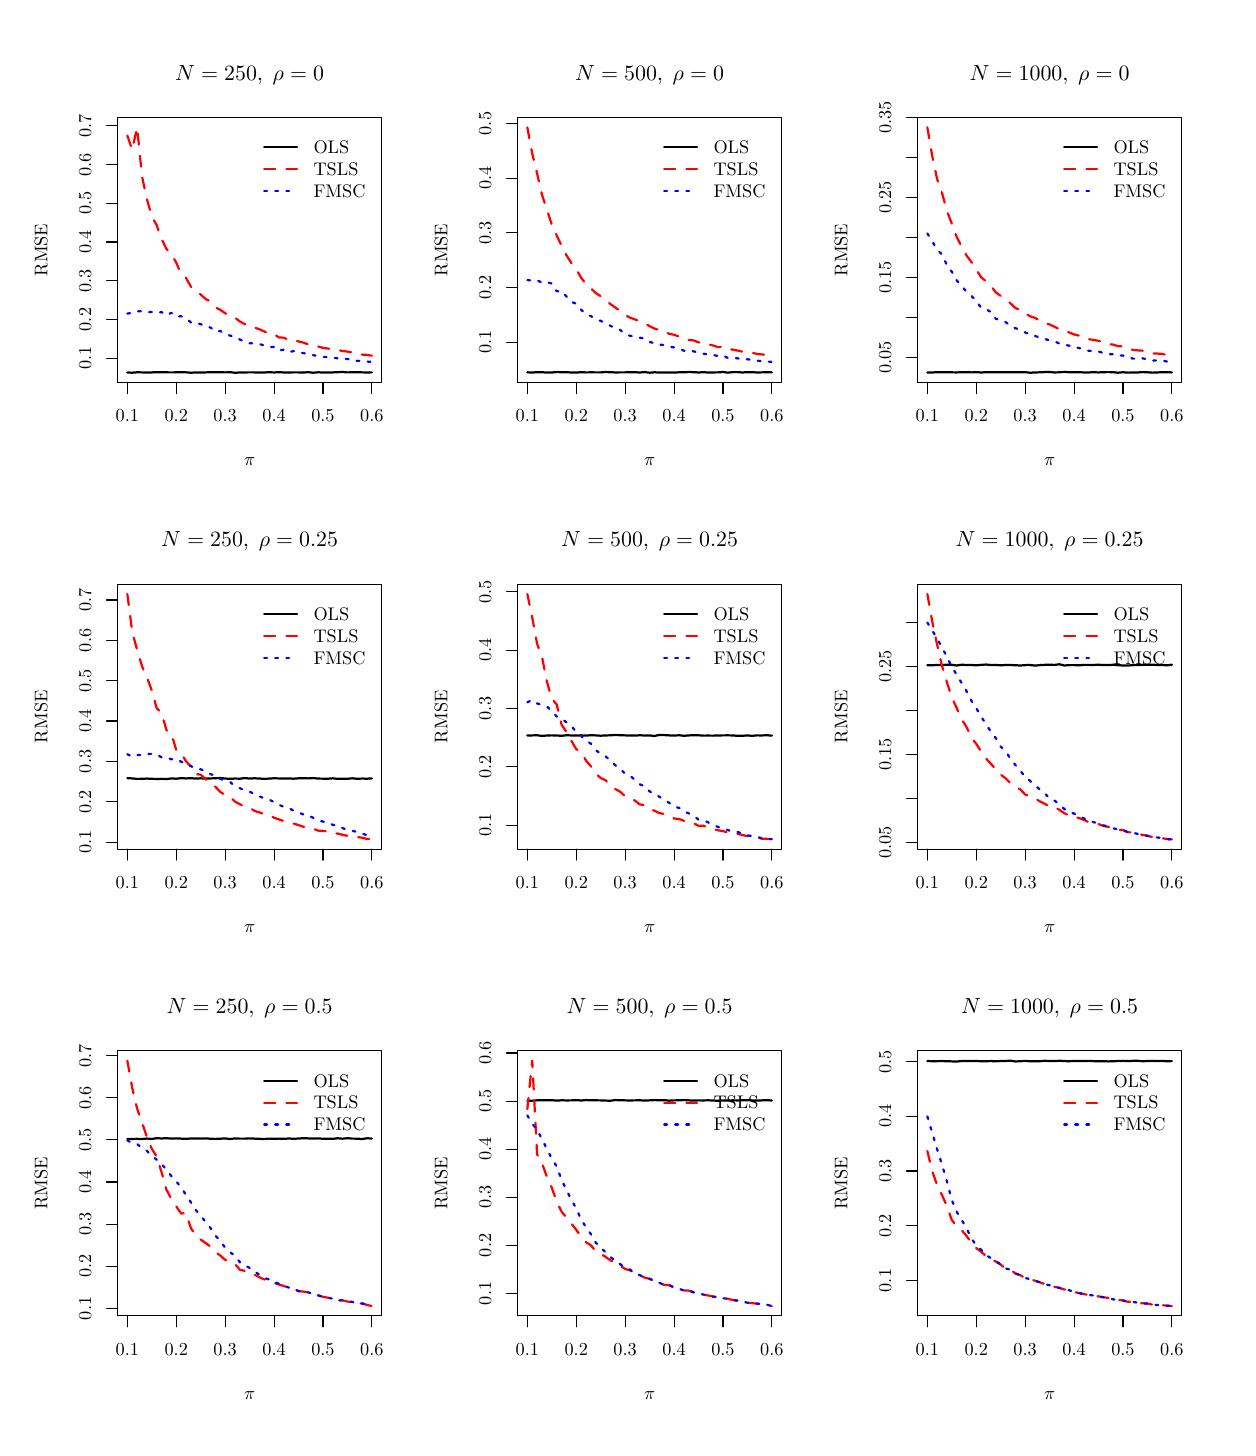
\begin{tikzpicture}[x=1pt,y=1pt]
\definecolor[named]{fillColor}{rgb}{1.00,1.00,1.00}
\path[use as bounding box,fill=fillColor,fill opacity=0.00] (0,0) rectangle (433.62,505.89);
\begin{scope}
\path[clip] ( 32.47,377.65) rectangle (127.91,473.42);
\definecolor[named]{drawColor}{rgb}{0.00,0.00,0.00}

\path[draw=drawColor,line width= 0.8pt,line join=round,line cap=round] ( 36.01,381.28) --
	( 37.77,381.21) --
	( 39.54,381.36) --
	( 41.31,381.32) --
	( 43.08,381.27) --
	( 44.84,381.31) --
	( 46.61,381.41) --
	( 48.38,381.34) --
	( 50.15,381.34) --
	( 51.91,381.32) --
	( 53.68,381.34) --
	( 55.45,381.35) --
	( 57.21,381.34) --
	( 58.98,381.20) --
	( 60.75,381.31) --
	( 62.52,381.29) --
	( 64.28,381.32) --
	( 66.05,381.38) --
	( 67.82,381.35) --
	( 69.59,381.41) --
	( 71.35,381.32) --
	( 73.12,381.40) --
	( 74.89,381.20) --
	( 76.66,381.27) --
	( 78.42,381.31) --
	( 80.19,381.33) --
	( 81.96,381.32) --
	( 83.72,381.27) --
	( 85.49,381.30) --
	( 87.26,381.38) --
	( 89.03,381.30) --
	( 90.79,381.39) --
	( 92.56,381.30) --
	( 94.33,381.29) --
	( 96.10,381.33) --
	( 97.86,381.32) --
	( 99.63,381.28) --
	(101.40,381.38) --
	(103.17,381.20) --
	(104.93,381.35) --
	(106.70,381.29) --
	(108.47,381.25) --
	(110.23,381.32) --
	(112.00,381.40) --
	(113.77,381.47) --
	(115.54,381.33) --
	(117.30,381.34) --
	(119.07,381.38) --
	(120.84,381.33) --
	(122.61,381.30) --
	(124.37,381.33);
\end{scope}
\begin{scope}
\path[clip] (  0.00,  0.00) rectangle (433.62,505.89);
\definecolor[named]{drawColor}{rgb}{0.00,0.00,0.00}

\path[draw=drawColor,line width= 0.4pt,line join=round,line cap=round] ( 36.01,377.65) -- (124.37,377.65);

\path[draw=drawColor,line width= 0.4pt,line join=round,line cap=round] ( 36.01,377.65) -- ( 36.01,373.69);

\path[draw=drawColor,line width= 0.4pt,line join=round,line cap=round] ( 53.68,377.65) -- ( 53.68,373.69);

\path[draw=drawColor,line width= 0.4pt,line join=round,line cap=round] ( 71.35,377.65) -- ( 71.35,373.69);

\path[draw=drawColor,line width= 0.4pt,line join=round,line cap=round] ( 89.03,377.65) -- ( 89.03,373.69);

\path[draw=drawColor,line width= 0.4pt,line join=round,line cap=round] (106.70,377.65) -- (106.70,373.69);

\path[draw=drawColor,line width= 0.4pt,line join=round,line cap=round] (124.37,377.65) -- (124.37,373.69);

\node[text=drawColor,anchor=base,inner sep=0pt, outer sep=0pt, scale=  0.66] at ( 36.01,363.40) {0.1};

\node[text=drawColor,anchor=base,inner sep=0pt, outer sep=0pt, scale=  0.66] at ( 53.68,363.40) {0.2};

\node[text=drawColor,anchor=base,inner sep=0pt, outer sep=0pt, scale=  0.66] at ( 71.35,363.40) {0.3};

\node[text=drawColor,anchor=base,inner sep=0pt, outer sep=0pt, scale=  0.66] at ( 89.03,363.40) {0.4};

\node[text=drawColor,anchor=base,inner sep=0pt, outer sep=0pt, scale=  0.66] at (106.70,363.40) {0.5};

\node[text=drawColor,anchor=base,inner sep=0pt, outer sep=0pt, scale=  0.66] at (124.37,363.40) {0.6};

\path[draw=drawColor,line width= 0.4pt,line join=round,line cap=round] ( 32.47,386.43) -- ( 32.47,470.42);

\path[draw=drawColor,line width= 0.4pt,line join=round,line cap=round] ( 32.47,386.43) -- ( 28.51,386.43);

\path[draw=drawColor,line width= 0.4pt,line join=round,line cap=round] ( 32.47,400.43) -- ( 28.51,400.43);

\path[draw=drawColor,line width= 0.4pt,line join=round,line cap=round] ( 32.47,414.43) -- ( 28.51,414.43);

\path[draw=drawColor,line width= 0.4pt,line join=round,line cap=round] ( 32.47,428.43) -- ( 28.51,428.43);

\path[draw=drawColor,line width= 0.4pt,line join=round,line cap=round] ( 32.47,442.43) -- ( 28.51,442.43);

\path[draw=drawColor,line width= 0.4pt,line join=round,line cap=round] ( 32.47,456.42) -- ( 28.51,456.42);

\path[draw=drawColor,line width= 0.4pt,line join=round,line cap=round] ( 32.47,470.42) -- ( 28.51,470.42);

\node[text=drawColor,rotate= 90.00,anchor=base,inner sep=0pt, outer sep=0pt, scale=  0.66] at ( 22.97,386.43) {0.1};

\node[text=drawColor,rotate= 90.00,anchor=base,inner sep=0pt, outer sep=0pt, scale=  0.66] at ( 22.97,400.43) {0.2};

\node[text=drawColor,rotate= 90.00,anchor=base,inner sep=0pt, outer sep=0pt, scale=  0.66] at ( 22.97,414.43) {0.3};

\node[text=drawColor,rotate= 90.00,anchor=base,inner sep=0pt, outer sep=0pt, scale=  0.66] at ( 22.97,428.43) {0.4};

\node[text=drawColor,rotate= 90.00,anchor=base,inner sep=0pt, outer sep=0pt, scale=  0.66] at ( 22.97,442.43) {0.5};

\node[text=drawColor,rotate= 90.00,anchor=base,inner sep=0pt, outer sep=0pt, scale=  0.66] at ( 22.97,456.42) {0.6};

\node[text=drawColor,rotate= 90.00,anchor=base,inner sep=0pt, outer sep=0pt, scale=  0.66] at ( 22.97,470.42) {0.7};

\path[draw=drawColor,line width= 0.4pt,line join=round,line cap=round] ( 32.47,377.65) --
	(127.91,377.65) --
	(127.91,473.42) --
	( 32.47,473.42) --
	( 32.47,377.65);
\end{scope}
\begin{scope}
\path[clip] (  0.00,337.26) rectangle (144.54,505.89);
\definecolor[named]{drawColor}{rgb}{0.00,0.00,0.00}

\node[text=drawColor,anchor=base,inner sep=0pt, outer sep=0pt, scale=  0.79] at ( 80.19,486.92) {\bfseries $N=250, \;\rho=0$};

\node[text=drawColor,anchor=base,inner sep=0pt, outer sep=0pt, scale=  0.66] at ( 80.19,347.56) {$\pi$};

\node[text=drawColor,rotate= 90.00,anchor=base,inner sep=0pt, outer sep=0pt, scale=  0.66] at (  7.13,425.53) {RMSE};
\end{scope}
\begin{scope}
\path[clip] ( 32.47,377.65) rectangle (127.91,473.42);
\definecolor[named]{drawColor}{rgb}{1.00,0.00,0.00}

\path[draw=drawColor,line width= 0.8pt,dash pattern=on 4pt off 4pt ,line join=round,line cap=round] ( 36.01,466.90) --
	( 37.77,461.77) --
	( 39.54,469.87) --
	( 41.31,452.21) --
	( 43.08,443.93) --
	( 44.84,437.71) --
	( 46.61,434.52) --
	( 48.38,429.50) --
	( 50.15,425.93) --
	( 51.91,424.10) --
	( 53.68,420.96) --
	( 55.45,416.99) --
	( 57.21,415.46) --
	( 58.98,412.33) --
	( 60.75,410.79) --
	( 62.52,409.47) --
	( 64.28,407.85) --
	( 66.05,406.94) --
	( 67.82,404.82) --
	( 69.59,403.93) --
	( 71.35,402.71) --
	( 73.12,401.68) --
	( 74.89,401.08) --
	( 76.66,399.74) --
	( 78.42,398.79) --
	( 80.19,397.80) --
	( 81.96,397.51) --
	( 83.72,396.91) --
	( 85.49,396.12) --
	( 87.26,395.31) --
	( 89.03,395.19) --
	( 90.79,393.94) --
	( 92.56,393.87) --
	( 94.33,393.00) --
	( 96.10,393.04) --
	( 97.86,392.50) --
	( 99.63,392.08) --
	(101.40,391.47) --
	(103.17,391.07) --
	(104.93,390.70) --
	(106.70,390.17) --
	(108.47,389.94) --
	(110.23,389.63) --
	(112.00,389.41) --
	(113.77,389.06) --
	(115.54,388.83) --
	(117.30,388.55) --
	(119.07,388.06) --
	(120.84,387.77) --
	(122.61,387.62) --
	(124.37,387.36);
\definecolor[named]{drawColor}{rgb}{0.00,0.00,1.00}

\path[draw=drawColor,line width= 0.8pt,dash pattern=on 1pt off 3pt ,line join=round,line cap=round] ( 36.01,402.56) --
	( 37.77,402.87) --
	( 39.54,403.36) --
	( 41.31,403.47) --
	( 43.08,403.12) --
	( 44.84,403.14) --
	( 46.61,402.82) --
	( 48.38,403.13) --
	( 50.15,401.89) --
	( 51.91,402.85) --
	( 53.68,401.46) --
	( 55.45,401.61) --
	( 57.21,400.92) --
	( 58.98,399.37) --
	( 60.75,399.19) --
	( 62.52,398.76) --
	( 64.28,397.82) --
	( 66.05,397.55) --
	( 67.82,396.06) --
	( 69.59,396.28) --
	( 71.35,395.10) --
	( 73.12,394.62) --
	( 74.89,394.18) --
	( 76.66,393.20) --
	( 78.42,392.47) --
	( 80.19,391.83) --
	( 81.96,391.79) --
	( 83.72,391.56) --
	( 85.49,391.06) --
	( 87.26,390.48) --
	( 89.03,390.54) --
	( 90.79,389.21) --
	( 92.56,389.54) --
	( 94.33,388.62) --
	( 96.10,389.01) --
	( 97.86,388.57) --
	( 99.63,388.29) --
	(101.40,387.97) --
	(103.17,387.55) --
	(104.93,387.18) --
	(106.70,386.95) --
	(108.47,386.80) --
	(110.23,386.52) --
	(112.00,386.45) --
	(113.77,386.35) --
	(115.54,386.13) --
	(117.30,386.00) --
	(119.07,385.50) --
	(120.84,385.44) --
	(122.61,385.24) --
	(124.37,385.10);
\definecolor[named]{drawColor}{rgb}{0.00,0.00,0.00}

\path[draw=drawColor,line width= 0.8pt,line join=round,line cap=round] ( 85.47,462.63) -- ( 97.35,462.63);
\definecolor[named]{drawColor}{rgb}{1.00,0.00,0.00}

\path[draw=drawColor,line width= 0.8pt,dash pattern=on 4pt off 4pt ,line join=round,line cap=round] ( 85.47,454.71) -- ( 97.35,454.71);
\definecolor[named]{drawColor}{rgb}{0.00,0.00,1.00}

\path[draw=drawColor,line width= 0.8pt,dash pattern=on 1pt off 3pt ,line join=round,line cap=round] ( 85.47,446.79) -- ( 97.35,446.79);
\definecolor[named]{drawColor}{rgb}{0.00,0.00,0.00}

\node[text=drawColor,anchor=base west,inner sep=0pt, outer sep=0pt, scale=  0.66] at (103.29,460.35) {OLS};

\node[text=drawColor,anchor=base west,inner sep=0pt, outer sep=0pt, scale=  0.66] at (103.29,452.43) {TSLS};

\node[text=drawColor,anchor=base west,inner sep=0pt, outer sep=0pt, scale=  0.66] at (103.29,444.51) {FMSC};
\end{scope}
\begin{scope}
\path[clip] (177.01,377.65) rectangle (272.45,473.42);
\definecolor[named]{drawColor}{rgb}{0.00,0.00,0.00}

\path[draw=drawColor,line width= 0.8pt,line join=round,line cap=round] (180.55,381.35) --
	(182.31,381.27) --
	(184.08,381.41) --
	(185.85,381.36) --
	(187.62,381.28) --
	(189.38,381.28) --
	(191.15,381.46) --
	(192.92,381.37) --
	(194.69,381.36) --
	(196.45,381.30) --
	(198.22,381.25) --
	(199.99,381.38) --
	(201.75,381.32) --
	(203.52,381.34) --
	(205.29,381.33) --
	(207.06,381.32) --
	(208.82,381.45) --
	(210.59,381.38) --
	(212.36,381.30) --
	(214.13,381.33) --
	(215.89,381.33) --
	(217.66,381.39) --
	(219.43,381.38) --
	(221.20,381.28) --
	(222.96,381.44) --
	(224.73,381.20) --
	(226.50,381.36) --
	(228.26,381.27) --
	(230.03,381.32) --
	(231.80,381.28) --
	(233.57,381.26) --
	(235.33,381.35) --
	(237.10,381.36) --
	(238.87,381.44) --
	(240.64,381.40) --
	(242.40,381.29) --
	(244.17,381.39) --
	(245.94,381.28) --
	(247.71,381.31) --
	(249.47,381.33) --
	(251.24,381.47) --
	(253.01,381.22) --
	(254.77,381.41) --
	(256.54,381.42) --
	(258.31,381.29) --
	(260.08,381.40) --
	(261.84,381.39) --
	(263.61,381.29) --
	(265.38,381.33) --
	(267.15,381.38) --
	(268.91,381.35);
\end{scope}
\begin{scope}
\path[clip] (  0.00,  0.00) rectangle (433.62,505.89);
\definecolor[named]{drawColor}{rgb}{0.00,0.00,0.00}

\path[draw=drawColor,line width= 0.4pt,line join=round,line cap=round] (180.55,377.65) -- (268.91,377.65);

\path[draw=drawColor,line width= 0.4pt,line join=round,line cap=round] (180.55,377.65) -- (180.55,373.69);

\path[draw=drawColor,line width= 0.4pt,line join=round,line cap=round] (198.22,377.65) -- (198.22,373.69);

\path[draw=drawColor,line width= 0.4pt,line join=round,line cap=round] (215.89,377.65) -- (215.89,373.69);

\path[draw=drawColor,line width= 0.4pt,line join=round,line cap=round] (233.57,377.65) -- (233.57,373.69);

\path[draw=drawColor,line width= 0.4pt,line join=round,line cap=round] (251.24,377.65) -- (251.24,373.69);

\path[draw=drawColor,line width= 0.4pt,line join=round,line cap=round] (268.91,377.65) -- (268.91,373.69);

\node[text=drawColor,anchor=base,inner sep=0pt, outer sep=0pt, scale=  0.66] at (180.55,363.40) {0.1};

\node[text=drawColor,anchor=base,inner sep=0pt, outer sep=0pt, scale=  0.66] at (198.22,363.40) {0.2};

\node[text=drawColor,anchor=base,inner sep=0pt, outer sep=0pt, scale=  0.66] at (215.89,363.40) {0.3};

\node[text=drawColor,anchor=base,inner sep=0pt, outer sep=0pt, scale=  0.66] at (233.57,363.40) {0.4};

\node[text=drawColor,anchor=base,inner sep=0pt, outer sep=0pt, scale=  0.66] at (251.24,363.40) {0.5};

\node[text=drawColor,anchor=base,inner sep=0pt, outer sep=0pt, scale=  0.66] at (268.91,363.40) {0.6};

\path[draw=drawColor,line width= 0.4pt,line join=round,line cap=round] (177.01,392.25) -- (177.01,471.27);

\path[draw=drawColor,line width= 0.4pt,line join=round,line cap=round] (177.01,392.25) -- (173.05,392.25);

\path[draw=drawColor,line width= 0.4pt,line join=round,line cap=round] (177.01,412.01) -- (173.05,412.01);

\path[draw=drawColor,line width= 0.4pt,line join=round,line cap=round] (177.01,431.76) -- (173.05,431.76);

\path[draw=drawColor,line width= 0.4pt,line join=round,line cap=round] (177.01,451.52) -- (173.05,451.52);

\path[draw=drawColor,line width= 0.4pt,line join=round,line cap=round] (177.01,471.27) -- (173.05,471.27);

\node[text=drawColor,rotate= 90.00,anchor=base,inner sep=0pt, outer sep=0pt, scale=  0.66] at (167.51,392.25) {0.1};

\node[text=drawColor,rotate= 90.00,anchor=base,inner sep=0pt, outer sep=0pt, scale=  0.66] at (167.51,412.01) {0.2};

\node[text=drawColor,rotate= 90.00,anchor=base,inner sep=0pt, outer sep=0pt, scale=  0.66] at (167.51,431.76) {0.3};

\node[text=drawColor,rotate= 90.00,anchor=base,inner sep=0pt, outer sep=0pt, scale=  0.66] at (167.51,451.52) {0.4};

\node[text=drawColor,rotate= 90.00,anchor=base,inner sep=0pt, outer sep=0pt, scale=  0.66] at (167.51,471.27) {0.5};

\path[draw=drawColor,line width= 0.4pt,line join=round,line cap=round] (177.01,377.65) --
	(272.45,377.65) --
	(272.45,473.42) --
	(177.01,473.42) --
	(177.01,377.65);
\end{scope}
\begin{scope}
\path[clip] (144.54,337.26) rectangle (289.08,505.89);
\definecolor[named]{drawColor}{rgb}{0.00,0.00,0.00}

\node[text=drawColor,anchor=base,inner sep=0pt, outer sep=0pt, scale=  0.79] at (224.73,486.92) {\bfseries $N=500, \;\rho=0$};

\node[text=drawColor,anchor=base,inner sep=0pt, outer sep=0pt, scale=  0.66] at (224.73,347.56) {$\pi$};

\node[text=drawColor,rotate= 90.00,anchor=base,inner sep=0pt, outer sep=0pt, scale=  0.66] at (151.67,425.53) {RMSE};
\end{scope}
\begin{scope}
\path[clip] (177.01,377.65) rectangle (272.45,473.42);
\definecolor[named]{drawColor}{rgb}{1.00,0.00,0.00}

\path[draw=drawColor,line width= 0.8pt,dash pattern=on 4pt off 4pt ,line join=round,line cap=round] (180.55,469.87) --
	(182.31,460.41) --
	(184.08,453.21) --
	(185.85,445.46) --
	(187.62,440.10) --
	(189.38,434.78) --
	(191.15,430.82) --
	(192.92,427.12) --
	(194.69,423.65) --
	(196.45,420.82) --
	(198.22,418.57) --
	(199.99,415.52) --
	(201.75,413.23) --
	(203.52,411.66) --
	(205.29,409.99) --
	(207.06,408.86) --
	(208.82,407.34) --
	(210.59,405.99) --
	(212.36,404.74) --
	(214.13,403.52) --
	(215.89,402.02) --
	(217.66,401.10) --
	(219.43,400.45) --
	(221.20,399.82) --
	(222.96,399.09) --
	(224.73,398.02) --
	(226.50,397.16) --
	(228.26,396.61) --
	(230.03,395.99) --
	(231.80,395.28) --
	(233.57,394.92) --
	(235.33,394.28) --
	(237.10,393.38) --
	(238.87,393.02) --
	(240.64,392.87) --
	(242.40,392.18) --
	(244.17,391.74) --
	(245.94,391.47) --
	(247.71,391.03) --
	(249.47,390.46) --
	(251.24,390.62) --
	(253.01,389.73) --
	(254.77,389.56) --
	(256.54,389.21) --
	(258.31,388.80) --
	(260.08,388.69) --
	(261.84,388.38) --
	(263.61,387.99) --
	(265.38,387.81) --
	(267.15,387.58) --
	(268.91,387.30);
\definecolor[named]{drawColor}{rgb}{0.00,0.00,1.00}

\path[draw=drawColor,line width= 0.8pt,dash pattern=on 1pt off 3pt ,line join=round,line cap=round] (180.55,414.68) --
	(182.31,414.53) --
	(184.08,414.62) --
	(185.85,413.72) --
	(187.62,413.92) --
	(189.38,413.42) --
	(191.15,410.65) --
	(192.92,410.73) --
	(194.69,408.76) --
	(196.45,406.83) --
	(198.22,406.11) --
	(199.99,403.96) --
	(201.75,402.36) --
	(203.52,401.66) --
	(205.29,400.62) --
	(207.06,399.93) --
	(208.82,399.12) --
	(210.59,398.13) --
	(212.36,397.28) --
	(214.13,396.65) --
	(215.89,395.09) --
	(217.66,394.54) --
	(219.43,394.23) --
	(221.20,393.85) --
	(222.96,393.49) --
	(224.73,392.33) --
	(226.50,391.84) --
	(228.26,391.36) --
	(230.03,391.19) --
	(231.80,390.58) --
	(233.57,390.34) --
	(235.33,389.94) --
	(237.10,389.16) --
	(238.87,388.91) --
	(240.64,388.94) --
	(242.40,388.37) --
	(244.17,388.05) --
	(245.94,387.86) --
	(247.71,387.63) --
	(249.47,387.22) --
	(251.24,387.39) --
	(253.01,386.54) --
	(254.77,386.69) --
	(256.54,386.39) --
	(258.31,385.99) --
	(260.08,386.07) --
	(261.84,385.77) --
	(263.61,385.53) --
	(265.38,385.40) --
	(267.15,385.29) --
	(268.91,385.10);
\definecolor[named]{drawColor}{rgb}{0.00,0.00,0.00}

\path[draw=drawColor,line width= 0.8pt,line join=round,line cap=round] (230.01,462.63) -- (241.89,462.63);
\definecolor[named]{drawColor}{rgb}{1.00,0.00,0.00}

\path[draw=drawColor,line width= 0.8pt,dash pattern=on 4pt off 4pt ,line join=round,line cap=round] (230.01,454.71) -- (241.89,454.71);
\definecolor[named]{drawColor}{rgb}{0.00,0.00,1.00}

\path[draw=drawColor,line width= 0.8pt,dash pattern=on 1pt off 3pt ,line join=round,line cap=round] (230.01,446.79) -- (241.89,446.79);
\definecolor[named]{drawColor}{rgb}{0.00,0.00,0.00}

\node[text=drawColor,anchor=base west,inner sep=0pt, outer sep=0pt, scale=  0.66] at (247.83,460.35) {OLS};

\node[text=drawColor,anchor=base west,inner sep=0pt, outer sep=0pt, scale=  0.66] at (247.83,452.43) {TSLS};

\node[text=drawColor,anchor=base west,inner sep=0pt, outer sep=0pt, scale=  0.66] at (247.83,444.51) {FMSC};
\end{scope}
\begin{scope}
\path[clip] (321.55,377.65) rectangle (416.99,473.42);
\definecolor[named]{drawColor}{rgb}{0.00,0.00,0.00}

\path[draw=drawColor,line width= 0.8pt,line join=round,line cap=round] (325.09,381.27) --
	(326.85,381.29) --
	(328.62,381.40) --
	(330.39,381.35) --
	(332.16,381.36) --
	(333.92,381.34) --
	(335.69,381.31) --
	(337.46,381.41) --
	(339.23,381.41) --
	(340.99,381.32) --
	(342.76,381.41) --
	(344.53,381.29) --
	(346.29,381.38) --
	(348.06,381.39) --
	(349.83,381.40) --
	(351.60,381.36) --
	(353.36,381.34) --
	(355.13,381.35) --
	(356.90,381.38) --
	(358.67,381.39) --
	(360.43,381.41) --
	(362.20,381.20) --
	(363.97,381.30) --
	(365.74,381.34) --
	(367.50,381.44) --
	(369.27,381.48) --
	(371.04,381.30) --
	(372.80,381.35) --
	(374.57,381.52) --
	(376.34,381.36) --
	(378.11,381.36) --
	(379.87,381.39) --
	(381.64,381.31) --
	(383.41,381.31) --
	(385.18,381.37) --
	(386.94,381.31) --
	(388.71,381.40) --
	(390.48,381.42) --
	(392.25,381.38) --
	(394.01,381.21) --
	(395.78,381.37) --
	(397.55,381.23) --
	(399.31,381.28) --
	(401.08,381.29) --
	(402.85,381.43) --
	(404.62,381.36) --
	(406.38,381.23) --
	(408.15,381.30) --
	(409.92,381.38) --
	(411.69,381.40) --
	(413.45,381.31);
\end{scope}
\begin{scope}
\path[clip] (  0.00,  0.00) rectangle (433.62,505.89);
\definecolor[named]{drawColor}{rgb}{0.00,0.00,0.00}

\path[draw=drawColor,line width= 0.4pt,line join=round,line cap=round] (325.09,377.65) -- (413.45,377.65);

\path[draw=drawColor,line width= 0.4pt,line join=round,line cap=round] (325.09,377.65) -- (325.09,373.69);

\path[draw=drawColor,line width= 0.4pt,line join=round,line cap=round] (342.76,377.65) -- (342.76,373.69);

\path[draw=drawColor,line width= 0.4pt,line join=round,line cap=round] (360.43,377.65) -- (360.43,373.69);

\path[draw=drawColor,line width= 0.4pt,line join=round,line cap=round] (378.11,377.65) -- (378.11,373.69);

\path[draw=drawColor,line width= 0.4pt,line join=round,line cap=round] (395.78,377.65) -- (395.78,373.69);

\path[draw=drawColor,line width= 0.4pt,line join=round,line cap=round] (413.45,377.65) -- (413.45,373.69);

\node[text=drawColor,anchor=base,inner sep=0pt, outer sep=0pt, scale=  0.66] at (325.09,363.40) {0.1};

\node[text=drawColor,anchor=base,inner sep=0pt, outer sep=0pt, scale=  0.66] at (342.76,363.40) {0.2};

\node[text=drawColor,anchor=base,inner sep=0pt, outer sep=0pt, scale=  0.66] at (360.43,363.40) {0.3};

\node[text=drawColor,anchor=base,inner sep=0pt, outer sep=0pt, scale=  0.66] at (378.11,363.40) {0.4};

\node[text=drawColor,anchor=base,inner sep=0pt, outer sep=0pt, scale=  0.66] at (395.78,363.40) {0.5};

\node[text=drawColor,anchor=base,inner sep=0pt, outer sep=0pt, scale=  0.66] at (413.45,363.40) {0.6};

\path[draw=drawColor,line width= 0.4pt,line join=round,line cap=round] (321.55,386.65) -- (321.55,473.35);

\path[draw=drawColor,line width= 0.4pt,line join=round,line cap=round] (321.55,386.65) -- (317.59,386.65);

\path[draw=drawColor,line width= 0.4pt,line join=round,line cap=round] (321.55,401.10) -- (317.59,401.10);

\path[draw=drawColor,line width= 0.4pt,line join=round,line cap=round] (321.55,415.55) -- (317.59,415.55);

\path[draw=drawColor,line width= 0.4pt,line join=round,line cap=round] (321.55,430.00) -- (317.59,430.00);

\path[draw=drawColor,line width= 0.4pt,line join=round,line cap=round] (321.55,444.45) -- (317.59,444.45);

\path[draw=drawColor,line width= 0.4pt,line join=round,line cap=round] (321.55,458.90) -- (317.59,458.90);

\path[draw=drawColor,line width= 0.4pt,line join=round,line cap=round] (321.55,473.35) -- (317.59,473.35);

\node[text=drawColor,rotate= 90.00,anchor=base,inner sep=0pt, outer sep=0pt, scale=  0.66] at (312.05,386.65) {0.05};

\node[text=drawColor,rotate= 90.00,anchor=base,inner sep=0pt, outer sep=0pt, scale=  0.66] at (312.05,415.55) {0.15};

\node[text=drawColor,rotate= 90.00,anchor=base,inner sep=0pt, outer sep=0pt, scale=  0.66] at (312.05,444.45) {0.25};

\node[text=drawColor,rotate= 90.00,anchor=base,inner sep=0pt, outer sep=0pt, scale=  0.66] at (312.05,473.35) {0.35};

\path[draw=drawColor,line width= 0.4pt,line join=round,line cap=round] (321.55,377.65) --
	(416.99,377.65) --
	(416.99,473.42) --
	(321.55,473.42) --
	(321.55,377.65);
\end{scope}
\begin{scope}
\path[clip] (289.08,337.26) rectangle (433.62,505.89);
\definecolor[named]{drawColor}{rgb}{0.00,0.00,0.00}

\node[text=drawColor,anchor=base,inner sep=0pt, outer sep=0pt, scale=  0.79] at (369.27,486.92) {\bfseries $N=1000, \;\rho=0$};

\node[text=drawColor,anchor=base,inner sep=0pt, outer sep=0pt, scale=  0.66] at (369.27,347.56) {$\pi$};

\node[text=drawColor,rotate= 90.00,anchor=base,inner sep=0pt, outer sep=0pt, scale=  0.66] at (296.21,425.53) {RMSE};
\end{scope}
\begin{scope}
\path[clip] (321.55,377.65) rectangle (416.99,473.42);
\definecolor[named]{drawColor}{rgb}{1.00,0.00,0.00}

\path[draw=drawColor,line width= 0.8pt,dash pattern=on 4pt off 4pt ,line join=round,line cap=round] (325.09,469.87) --
	(326.85,459.55) --
	(328.62,451.20) --
	(330.39,446.20) --
	(332.16,439.70) --
	(333.92,435.07) --
	(335.69,430.30) --
	(337.46,426.80) --
	(339.23,423.59) --
	(340.99,421.24) --
	(342.76,418.49) --
	(344.53,415.67) --
	(346.29,414.26) --
	(348.06,412.60) --
	(349.83,410.21) --
	(351.60,408.99) --
	(353.36,407.81) --
	(355.13,406.28) --
	(356.90,404.59) --
	(358.67,403.90) --
	(360.43,402.60) --
	(362.20,401.63) --
	(363.97,401.04) --
	(365.74,400.01) --
	(367.50,399.22) --
	(369.27,398.62) --
	(371.04,397.80) --
	(372.80,396.92) --
	(374.57,396.26) --
	(376.34,395.75) --
	(378.11,395.05) --
	(379.87,394.60) --
	(381.64,393.84) --
	(383.41,393.32) --
	(385.18,393.04) --
	(386.94,392.74) --
	(388.71,392.11) --
	(390.48,391.59) --
	(392.25,391.35) --
	(394.01,390.80) --
	(395.78,390.67) --
	(397.55,390.24) --
	(399.31,389.45) --
	(401.08,389.28) --
	(402.85,389.17) --
	(404.62,388.81) --
	(406.38,388.21) --
	(408.15,388.12) --
	(409.92,387.99) --
	(411.69,387.57) --
	(413.45,387.36);
\definecolor[named]{drawColor}{rgb}{0.00,0.00,1.00}

\path[draw=drawColor,line width= 0.8pt,dash pattern=on 1pt off 3pt ,line join=round,line cap=round] (325.09,431.52) --
	(326.85,428.76) --
	(328.62,425.55) --
	(330.39,423.97) --
	(332.16,420.11) --
	(333.92,417.72) --
	(335.69,414.57) --
	(337.46,412.58) --
	(339.23,410.45) --
	(340.99,408.96) --
	(342.76,407.18) --
	(344.53,404.61) --
	(346.29,404.17) --
	(348.06,403.13) --
	(349.83,400.69) --
	(351.60,400.18) --
	(353.36,399.48) --
	(355.13,398.16) --
	(356.90,397.27) --
	(358.67,396.79) --
	(360.43,395.77) --
	(362.20,395.05) --
	(363.97,394.50) --
	(365.74,393.93) --
	(367.50,393.42) --
	(369.27,392.86) --
	(371.04,392.54) --
	(372.80,391.74) --
	(374.57,391.36) --
	(376.34,390.96) --
	(378.11,390.35) --
	(379.87,390.16) --
	(381.64,389.41) --
	(383.41,389.12) --
	(385.18,389.04) --
	(386.94,388.88) --
	(388.71,388.28) --
	(390.48,387.92) --
	(392.25,387.87) --
	(394.01,387.46) --
	(395.78,387.39) --
	(397.55,387.12) --
	(399.31,386.29) --
	(401.08,386.32) --
	(402.85,386.40) --
	(404.62,386.00) --
	(406.38,385.64) --
	(408.15,385.66) --
	(409.92,385.59) --
	(411.69,385.23) --
	(413.45,385.09);
\definecolor[named]{drawColor}{rgb}{0.00,0.00,0.00}

\path[draw=drawColor,line width= 0.8pt,line join=round,line cap=round] (374.55,462.63) -- (386.43,462.63);
\definecolor[named]{drawColor}{rgb}{1.00,0.00,0.00}

\path[draw=drawColor,line width= 0.8pt,dash pattern=on 4pt off 4pt ,line join=round,line cap=round] (374.55,454.71) -- (386.43,454.71);
\definecolor[named]{drawColor}{rgb}{0.00,0.00,1.00}

\path[draw=drawColor,line width= 0.8pt,dash pattern=on 1pt off 3pt ,line join=round,line cap=round] (374.55,446.79) -- (386.43,446.79);
\definecolor[named]{drawColor}{rgb}{0.00,0.00,0.00}

\node[text=drawColor,anchor=base west,inner sep=0pt, outer sep=0pt, scale=  0.66] at (392.37,460.35) {OLS};

\node[text=drawColor,anchor=base west,inner sep=0pt, outer sep=0pt, scale=  0.66] at (392.37,452.43) {TSLS};

\node[text=drawColor,anchor=base west,inner sep=0pt, outer sep=0pt, scale=  0.66] at (392.37,444.51) {FMSC};
\end{scope}
\begin{scope}
\path[clip] ( 32.47,209.02) rectangle (127.91,304.79);
\definecolor[named]{drawColor}{rgb}{0.00,0.00,0.00}

\path[draw=drawColor,line width= 0.8pt,line join=round,line cap=round] ( 36.01,234.72) --
	( 37.77,234.60) --
	( 39.54,234.43) --
	( 41.31,234.46) --
	( 43.08,234.55) --
	( 44.84,234.47) --
	( 46.61,234.40) --
	( 48.38,234.45) --
	( 50.15,234.38) --
	( 51.91,234.59) --
	( 53.68,234.50) --
	( 55.45,234.69) --
	( 57.21,234.60) --
	( 58.98,234.70) --
	( 60.75,234.55) --
	( 62.52,234.64) --
	( 64.28,234.54) --
	( 66.05,234.61) --
	( 67.82,234.65) --
	( 69.59,234.75) --
	( 71.35,234.57) --
	( 73.12,234.45) --
	( 74.89,234.56) --
	( 76.66,234.50) --
	( 78.42,234.73) --
	( 80.19,234.56) --
	( 81.96,234.65) --
	( 83.72,234.57) --
	( 85.49,234.43) --
	( 87.26,234.55) --
	( 89.03,234.65) --
	( 90.79,234.61) --
	( 92.56,234.56) --
	( 94.33,234.58) --
	( 96.10,234.51) --
	( 97.86,234.64) --
	( 99.63,234.66) --
	(101.40,234.62) --
	(103.17,234.73) --
	(104.93,234.55) --
	(106.70,234.52) --
	(108.47,234.49) --
	(110.23,234.64) --
	(112.00,234.44) --
	(113.77,234.51) --
	(115.54,234.46) --
	(117.30,234.65) --
	(119.07,234.47) --
	(120.84,234.55) --
	(122.61,234.50) --
	(124.37,234.62);
\end{scope}
\begin{scope}
\path[clip] (  0.00,  0.00) rectangle (433.62,505.89);
\definecolor[named]{drawColor}{rgb}{0.00,0.00,0.00}

\path[draw=drawColor,line width= 0.4pt,line join=round,line cap=round] ( 36.01,209.02) -- (124.37,209.02);

\path[draw=drawColor,line width= 0.4pt,line join=round,line cap=round] ( 36.01,209.02) -- ( 36.01,205.06);

\path[draw=drawColor,line width= 0.4pt,line join=round,line cap=round] ( 53.68,209.02) -- ( 53.68,205.06);

\path[draw=drawColor,line width= 0.4pt,line join=round,line cap=round] ( 71.35,209.02) -- ( 71.35,205.06);

\path[draw=drawColor,line width= 0.4pt,line join=round,line cap=round] ( 89.03,209.02) -- ( 89.03,205.06);

\path[draw=drawColor,line width= 0.4pt,line join=round,line cap=round] (106.70,209.02) -- (106.70,205.06);

\path[draw=drawColor,line width= 0.4pt,line join=round,line cap=round] (124.37,209.02) -- (124.37,205.06);

\node[text=drawColor,anchor=base,inner sep=0pt, outer sep=0pt, scale=  0.66] at ( 36.01,194.77) {0.1};

\node[text=drawColor,anchor=base,inner sep=0pt, outer sep=0pt, scale=  0.66] at ( 53.68,194.77) {0.2};

\node[text=drawColor,anchor=base,inner sep=0pt, outer sep=0pt, scale=  0.66] at ( 71.35,194.77) {0.3};

\node[text=drawColor,anchor=base,inner sep=0pt, outer sep=0pt, scale=  0.66] at ( 89.03,194.77) {0.4};

\node[text=drawColor,anchor=base,inner sep=0pt, outer sep=0pt, scale=  0.66] at (106.70,194.77) {0.5};

\node[text=drawColor,anchor=base,inner sep=0pt, outer sep=0pt, scale=  0.66] at (124.37,194.77) {0.6};

\path[draw=drawColor,line width= 0.4pt,line join=round,line cap=round] ( 32.47,211.61) -- ( 32.47,299.08);

\path[draw=drawColor,line width= 0.4pt,line join=round,line cap=round] ( 32.47,211.61) -- ( 28.51,211.61);

\path[draw=drawColor,line width= 0.4pt,line join=round,line cap=round] ( 32.47,226.18) -- ( 28.51,226.18);

\path[draw=drawColor,line width= 0.4pt,line join=round,line cap=round] ( 32.47,240.76) -- ( 28.51,240.76);

\path[draw=drawColor,line width= 0.4pt,line join=round,line cap=round] ( 32.47,255.34) -- ( 28.51,255.34);

\path[draw=drawColor,line width= 0.4pt,line join=round,line cap=round] ( 32.47,269.92) -- ( 28.51,269.92);

\path[draw=drawColor,line width= 0.4pt,line join=round,line cap=round] ( 32.47,284.50) -- ( 28.51,284.50);

\path[draw=drawColor,line width= 0.4pt,line join=round,line cap=round] ( 32.47,299.08) -- ( 28.51,299.08);

\node[text=drawColor,rotate= 90.00,anchor=base,inner sep=0pt, outer sep=0pt, scale=  0.66] at ( 22.97,211.61) {0.1};

\node[text=drawColor,rotate= 90.00,anchor=base,inner sep=0pt, outer sep=0pt, scale=  0.66] at ( 22.97,226.18) {0.2};

\node[text=drawColor,rotate= 90.00,anchor=base,inner sep=0pt, outer sep=0pt, scale=  0.66] at ( 22.97,240.76) {0.3};

\node[text=drawColor,rotate= 90.00,anchor=base,inner sep=0pt, outer sep=0pt, scale=  0.66] at ( 22.97,255.34) {0.4};

\node[text=drawColor,rotate= 90.00,anchor=base,inner sep=0pt, outer sep=0pt, scale=  0.66] at ( 22.97,269.92) {0.5};

\node[text=drawColor,rotate= 90.00,anchor=base,inner sep=0pt, outer sep=0pt, scale=  0.66] at ( 22.97,284.50) {0.6};

\node[text=drawColor,rotate= 90.00,anchor=base,inner sep=0pt, outer sep=0pt, scale=  0.66] at ( 22.97,299.08) {0.7};

\path[draw=drawColor,line width= 0.4pt,line join=round,line cap=round] ( 32.47,209.02) --
	(127.91,209.02) --
	(127.91,304.79) --
	( 32.47,304.79) --
	( 32.47,209.02);
\end{scope}
\begin{scope}
\path[clip] (  0.00,168.63) rectangle (144.54,337.26);
\definecolor[named]{drawColor}{rgb}{0.00,0.00,0.00}

\node[text=drawColor,anchor=base,inner sep=0pt, outer sep=0pt, scale=  0.79] at ( 80.19,318.29) {\bfseries $N=250, \;\rho=0.25$};

\node[text=drawColor,anchor=base,inner sep=0pt, outer sep=0pt, scale=  0.66] at ( 80.19,178.93) {$\pi$};

\node[text=drawColor,rotate= 90.00,anchor=base,inner sep=0pt, outer sep=0pt, scale=  0.66] at (  7.13,256.90) {RMSE};
\end{scope}
\begin{scope}
\path[clip] ( 32.47,209.02) rectangle (127.91,304.79);
\definecolor[named]{drawColor}{rgb}{1.00,0.00,0.00}

\path[draw=drawColor,line width= 0.8pt,dash pattern=on 4pt off 4pt ,line join=round,line cap=round] ( 36.01,301.24) --
	( 37.77,287.60) --
	( 39.54,281.05) --
	( 41.31,275.17) --
	( 43.08,271.14) --
	( 44.84,266.48) --
	( 46.61,260.00) --
	( 48.38,258.23) --
	( 50.15,252.04) --
	( 51.91,250.91) --
	( 53.68,244.88) --
	( 55.45,243.78) --
	( 57.21,240.79) --
	( 58.98,238.90) --
	( 60.75,236.17) --
	( 62.52,235.97) --
	( 64.28,234.34) --
	( 66.05,232.79) --
	( 67.82,231.59) --
	( 69.59,229.72) --
	( 71.35,228.60) --
	( 73.12,228.02) --
	( 74.89,226.24) --
	( 76.66,225.27) --
	( 78.42,224.56) --
	( 80.19,224.01) --
	( 81.96,222.88) --
	( 83.72,222.31) --
	( 85.49,221.68) --
	( 87.26,221.42) --
	( 89.03,220.41) --
	( 90.79,219.80) --
	( 92.56,219.17) --
	( 94.33,218.71) --
	( 96.10,218.29) --
	( 97.86,217.73) --
	( 99.63,217.15) --
	(101.40,217.04) --
	(103.17,216.43) --
	(104.93,215.74) --
	(106.70,215.64) --
	(108.47,215.42) --
	(110.23,214.94) --
	(112.00,214.66) --
	(113.77,214.24) --
	(115.54,213.86) --
	(117.30,213.67) --
	(119.07,213.45) --
	(120.84,213.16) --
	(122.61,212.74) --
	(124.37,212.57);
\definecolor[named]{drawColor}{rgb}{0.00,0.00,1.00}

\path[draw=drawColor,line width= 0.8pt,dash pattern=on 1pt off 3pt ,line join=round,line cap=round] ( 36.01,243.37) --
	( 37.77,242.42) --
	( 39.54,243.06) --
	( 41.31,243.09) --
	( 43.08,243.34) --
	( 44.84,243.49) --
	( 46.61,243.15) --
	( 48.38,242.25) --
	( 50.15,242.21) --
	( 51.91,241.53) --
	( 53.68,241.72) --
	( 55.45,240.65) --
	( 57.21,239.57) --
	( 58.98,239.09) --
	( 60.75,237.99) --
	( 62.52,237.89) --
	( 64.28,237.22) --
	( 66.05,236.17) --
	( 67.82,235.55) --
	( 69.59,234.45) --
	( 71.35,233.83) --
	( 73.12,233.35) --
	( 74.89,231.82) --
	( 76.66,231.08) --
	( 78.42,230.27) --
	( 80.19,229.80) --
	( 81.96,228.98) --
	( 83.72,228.14) --
	( 85.49,227.38) --
	( 87.26,226.95) --
	( 89.03,226.07) --
	( 90.79,225.10) --
	( 92.56,224.31) --
	( 94.33,223.87) --
	( 96.10,222.98) --
	( 97.86,222.34) --
	( 99.63,221.57) --
	(101.40,221.34) --
	(103.17,220.35) --
	(104.93,219.38) --
	(106.70,219.02) --
	(108.47,218.51) --
	(110.23,217.88) --
	(112.00,217.30) --
	(113.77,216.66) --
	(115.54,215.98) --
	(117.30,215.70) --
	(119.07,215.21) --
	(120.84,214.63) --
	(122.61,214.13) --
	(124.37,213.72);
\definecolor[named]{drawColor}{rgb}{0.00,0.00,0.00}

\path[draw=drawColor,line width= 0.8pt,line join=round,line cap=round] ( 85.47,294.00) -- ( 97.35,294.00);
\definecolor[named]{drawColor}{rgb}{1.00,0.00,0.00}

\path[draw=drawColor,line width= 0.8pt,dash pattern=on 4pt off 4pt ,line join=round,line cap=round] ( 85.47,286.08) -- ( 97.35,286.08);
\definecolor[named]{drawColor}{rgb}{0.00,0.00,1.00}

\path[draw=drawColor,line width= 0.8pt,dash pattern=on 1pt off 3pt ,line join=round,line cap=round] ( 85.47,278.16) -- ( 97.35,278.16);
\definecolor[named]{drawColor}{rgb}{0.00,0.00,0.00}

\node[text=drawColor,anchor=base west,inner sep=0pt, outer sep=0pt, scale=  0.66] at (103.29,291.72) {OLS};

\node[text=drawColor,anchor=base west,inner sep=0pt, outer sep=0pt, scale=  0.66] at (103.29,283.80) {TSLS};

\node[text=drawColor,anchor=base west,inner sep=0pt, outer sep=0pt, scale=  0.66] at (103.29,275.88) {FMSC};
\end{scope}
\begin{scope}
\path[clip] (177.01,209.02) rectangle (272.45,304.79);
\definecolor[named]{drawColor}{rgb}{0.00,0.00,0.00}

\path[draw=drawColor,line width= 0.8pt,line join=round,line cap=round] (180.55,250.12) --
	(182.31,250.15) --
	(184.08,250.20) --
	(185.85,249.96) --
	(187.62,250.11) --
	(189.38,250.16) --
	(191.15,250.12) --
	(192.92,250.00) --
	(194.69,250.20) --
	(196.45,250.14) --
	(198.22,250.12) --
	(199.99,250.17) --
	(201.75,250.10) --
	(203.52,250.20) --
	(205.29,250.15) --
	(207.06,250.04) --
	(208.82,250.13) --
	(210.59,250.18) --
	(212.36,250.32) --
	(214.13,250.20) --
	(215.89,250.16) --
	(217.66,250.08) --
	(219.43,250.09) --
	(221.20,250.19) --
	(222.96,250.12) --
	(224.73,250.14) --
	(226.50,249.94) --
	(228.26,250.33) --
	(230.03,250.26) --
	(231.80,250.16) --
	(233.57,250.07) --
	(235.33,250.21) --
	(237.10,250.01) --
	(238.87,250.14) --
	(240.64,250.23) --
	(242.40,250.19) --
	(244.17,250.07) --
	(245.94,250.08) --
	(247.71,250.06) --
	(249.47,250.12) --
	(251.24,250.16) --
	(253.01,250.17) --
	(254.77,250.14) --
	(256.54,250.00) --
	(258.31,250.02) --
	(260.08,250.13) --
	(261.84,250.00) --
	(263.61,250.16) --
	(265.38,250.14) --
	(267.15,250.21) --
	(268.91,250.06);
\end{scope}
\begin{scope}
\path[clip] (  0.00,  0.00) rectangle (433.62,505.89);
\definecolor[named]{drawColor}{rgb}{0.00,0.00,0.00}

\path[draw=drawColor,line width= 0.4pt,line join=round,line cap=round] (180.55,209.02) -- (268.91,209.02);

\path[draw=drawColor,line width= 0.4pt,line join=round,line cap=round] (180.55,209.02) -- (180.55,205.06);

\path[draw=drawColor,line width= 0.4pt,line join=round,line cap=round] (198.22,209.02) -- (198.22,205.06);

\path[draw=drawColor,line width= 0.4pt,line join=round,line cap=round] (215.89,209.02) -- (215.89,205.06);

\path[draw=drawColor,line width= 0.4pt,line join=round,line cap=round] (233.57,209.02) -- (233.57,205.06);

\path[draw=drawColor,line width= 0.4pt,line join=round,line cap=round] (251.24,209.02) -- (251.24,205.06);

\path[draw=drawColor,line width= 0.4pt,line join=round,line cap=round] (268.91,209.02) -- (268.91,205.06);

\node[text=drawColor,anchor=base,inner sep=0pt, outer sep=0pt, scale=  0.66] at (180.55,194.77) {0.1};

\node[text=drawColor,anchor=base,inner sep=0pt, outer sep=0pt, scale=  0.66] at (198.22,194.77) {0.2};

\node[text=drawColor,anchor=base,inner sep=0pt, outer sep=0pt, scale=  0.66] at (215.89,194.77) {0.3};

\node[text=drawColor,anchor=base,inner sep=0pt, outer sep=0pt, scale=  0.66] at (233.57,194.77) {0.4};

\node[text=drawColor,anchor=base,inner sep=0pt, outer sep=0pt, scale=  0.66] at (251.24,194.77) {0.5};

\node[text=drawColor,anchor=base,inner sep=0pt, outer sep=0pt, scale=  0.66] at (268.91,194.77) {0.6};

\path[draw=drawColor,line width= 0.4pt,line join=round,line cap=round] (177.01,217.74) -- (177.01,302.02);

\path[draw=drawColor,line width= 0.4pt,line join=round,line cap=round] (177.01,217.74) -- (173.05,217.74);

\path[draw=drawColor,line width= 0.4pt,line join=round,line cap=round] (177.01,238.81) -- (173.05,238.81);

\path[draw=drawColor,line width= 0.4pt,line join=round,line cap=round] (177.01,259.88) -- (173.05,259.88);

\path[draw=drawColor,line width= 0.4pt,line join=round,line cap=round] (177.01,280.95) -- (173.05,280.95);

\path[draw=drawColor,line width= 0.4pt,line join=round,line cap=round] (177.01,302.02) -- (173.05,302.02);

\node[text=drawColor,rotate= 90.00,anchor=base,inner sep=0pt, outer sep=0pt, scale=  0.66] at (167.51,217.74) {0.1};

\node[text=drawColor,rotate= 90.00,anchor=base,inner sep=0pt, outer sep=0pt, scale=  0.66] at (167.51,238.81) {0.2};

\node[text=drawColor,rotate= 90.00,anchor=base,inner sep=0pt, outer sep=0pt, scale=  0.66] at (167.51,259.88) {0.3};

\node[text=drawColor,rotate= 90.00,anchor=base,inner sep=0pt, outer sep=0pt, scale=  0.66] at (167.51,280.95) {0.4};

\node[text=drawColor,rotate= 90.00,anchor=base,inner sep=0pt, outer sep=0pt, scale=  0.66] at (167.51,302.02) {0.5};

\path[draw=drawColor,line width= 0.4pt,line join=round,line cap=round] (177.01,209.02) --
	(272.45,209.02) --
	(272.45,304.79) --
	(177.01,304.79) --
	(177.01,209.02);
\end{scope}
\begin{scope}
\path[clip] (144.54,168.63) rectangle (289.08,337.26);
\definecolor[named]{drawColor}{rgb}{0.00,0.00,0.00}

\node[text=drawColor,anchor=base,inner sep=0pt, outer sep=0pt, scale=  0.79] at (224.73,318.29) {\bfseries $N=500, \;\rho=0.25$};

\node[text=drawColor,anchor=base,inner sep=0pt, outer sep=0pt, scale=  0.66] at (224.73,178.93) {$\pi$};

\node[text=drawColor,rotate= 90.00,anchor=base,inner sep=0pt, outer sep=0pt, scale=  0.66] at (151.67,256.90) {RMSE};
\end{scope}
\begin{scope}
\path[clip] (177.01,209.02) rectangle (272.45,304.79);
\definecolor[named]{drawColor}{rgb}{1.00,0.00,0.00}

\path[draw=drawColor,line width= 0.8pt,dash pattern=on 4pt off 4pt ,line join=round,line cap=round] (180.55,301.24) --
	(182.31,292.78) --
	(184.08,283.24) --
	(185.85,278.53) --
	(187.62,269.57) --
	(189.38,263.35) --
	(191.15,261.36) --
	(192.92,254.05) --
	(194.69,251.35) --
	(196.45,248.21) --
	(198.22,245.19) --
	(199.99,244.13) --
	(201.75,241.04) --
	(203.52,238.98) --
	(205.29,236.31) --
	(207.06,234.76) --
	(208.82,233.94) --
	(210.59,232.24) --
	(212.36,230.74) --
	(214.13,229.77) --
	(215.89,228.12) --
	(217.66,227.60) --
	(219.43,226.56) --
	(221.20,225.19) --
	(222.96,224.98) --
	(224.73,223.48) --
	(226.50,222.93) --
	(228.26,222.09) --
	(230.03,221.72) --
	(231.80,221.03) --
	(233.57,220.13) --
	(235.33,219.93) --
	(237.10,219.32) --
	(238.87,218.83) --
	(240.64,218.44) --
	(242.40,217.45) --
	(244.17,217.49) --
	(245.94,216.90) --
	(247.71,216.34) --
	(249.47,215.84) --
	(251.24,215.56) --
	(253.01,215.07) --
	(254.77,214.56) --
	(256.54,214.59) --
	(258.31,214.15) --
	(260.08,213.76) --
	(261.84,213.51) --
	(263.61,213.31) --
	(265.38,212.80) --
	(267.15,212.77) --
	(268.91,212.57);
\definecolor[named]{drawColor}{rgb}{0.00,0.00,1.00}

\path[draw=drawColor,line width= 0.8pt,dash pattern=on 1pt off 3pt ,line join=round,line cap=round] (180.55,262.12) --
	(182.31,262.92) --
	(184.08,261.70) --
	(185.85,261.11) --
	(187.62,260.62) --
	(189.38,258.83) --
	(191.15,257.00) --
	(192.92,256.23) --
	(194.69,254.86) --
	(196.45,253.56) --
	(198.22,251.36) --
	(199.99,249.94) --
	(201.75,248.35) --
	(203.52,247.15) --
	(205.29,244.82) --
	(207.06,243.51) --
	(208.82,242.60) --
	(210.59,240.91) --
	(212.36,239.37) --
	(214.13,238.06) --
	(215.89,236.31) --
	(217.66,235.59) --
	(219.43,234.05) --
	(221.20,232.49) --
	(222.96,231.74) --
	(224.73,229.94) --
	(226.50,228.96) --
	(228.26,227.97) --
	(230.03,226.77) --
	(231.80,225.80) --
	(233.57,224.36) --
	(235.33,223.97) --
	(237.10,222.77) --
	(238.87,221.95) --
	(240.64,221.14) --
	(242.40,219.72) --
	(244.17,219.58) --
	(245.94,218.67) --
	(247.71,217.90) --
	(249.47,217.04) --
	(251.24,216.54) --
	(253.01,215.97) --
	(254.77,215.26) --
	(256.54,215.24) --
	(258.31,214.67) --
	(260.08,214.08) --
	(261.84,213.73) --
	(263.61,213.52) --
	(265.38,212.94) --
	(267.15,212.84) --
	(268.91,212.65);
\definecolor[named]{drawColor}{rgb}{0.00,0.00,0.00}

\path[draw=drawColor,line width= 0.8pt,line join=round,line cap=round] (230.01,294.00) -- (241.89,294.00);
\definecolor[named]{drawColor}{rgb}{1.00,0.00,0.00}

\path[draw=drawColor,line width= 0.8pt,dash pattern=on 4pt off 4pt ,line join=round,line cap=round] (230.01,286.08) -- (241.89,286.08);
\definecolor[named]{drawColor}{rgb}{0.00,0.00,1.00}

\path[draw=drawColor,line width= 0.8pt,dash pattern=on 1pt off 3pt ,line join=round,line cap=round] (230.01,278.16) -- (241.89,278.16);
\definecolor[named]{drawColor}{rgb}{0.00,0.00,0.00}

\node[text=drawColor,anchor=base west,inner sep=0pt, outer sep=0pt, scale=  0.66] at (247.83,291.72) {OLS};

\node[text=drawColor,anchor=base west,inner sep=0pt, outer sep=0pt, scale=  0.66] at (247.83,283.80) {TSLS};

\node[text=drawColor,anchor=base west,inner sep=0pt, outer sep=0pt, scale=  0.66] at (247.83,275.88) {FMSC};
\end{scope}
\begin{scope}
\path[clip] (321.55,209.02) rectangle (416.99,304.79);
\definecolor[named]{drawColor}{rgb}{0.00,0.00,0.00}

\path[draw=drawColor,line width= 0.8pt,line join=round,line cap=round] (325.09,275.52) --
	(326.85,275.50) --
	(328.62,275.59) --
	(330.39,275.60) --
	(332.16,275.67) --
	(333.92,275.66) --
	(335.69,275.41) --
	(337.46,275.68) --
	(339.23,275.60) --
	(340.99,275.58) --
	(342.76,275.50) --
	(344.53,275.63) --
	(346.29,275.75) --
	(348.06,275.59) --
	(349.83,275.62) --
	(351.60,275.48) --
	(353.36,275.58) --
	(355.13,275.58) --
	(356.90,275.51) --
	(358.67,275.41) --
	(360.43,275.54) --
	(362.20,275.59) --
	(363.97,275.37) --
	(365.74,275.55) --
	(367.50,275.64) --
	(369.27,275.72) --
	(371.04,275.61) --
	(372.80,275.86) --
	(374.57,275.41) --
	(376.34,275.54) --
	(378.11,275.55) --
	(379.87,275.46) --
	(381.64,275.64) --
	(383.41,275.63) --
	(385.18,275.61) --
	(386.94,275.69) --
	(388.71,275.55) --
	(390.48,275.57) --
	(392.25,275.67) --
	(394.01,275.52) --
	(395.78,275.42) --
	(397.55,275.39) --
	(399.31,275.54) --
	(401.08,275.61) --
	(402.85,275.63) --
	(404.62,275.66) --
	(406.38,275.69) --
	(408.15,275.59) --
	(409.92,275.59) --
	(411.69,275.46) --
	(413.45,275.69);
\end{scope}
\begin{scope}
\path[clip] (  0.00,  0.00) rectangle (433.62,505.89);
\definecolor[named]{drawColor}{rgb}{0.00,0.00,0.00}

\path[draw=drawColor,line width= 0.4pt,line join=round,line cap=round] (325.09,209.02) -- (413.45,209.02);

\path[draw=drawColor,line width= 0.4pt,line join=round,line cap=round] (325.09,209.02) -- (325.09,205.06);

\path[draw=drawColor,line width= 0.4pt,line join=round,line cap=round] (342.76,209.02) -- (342.76,205.06);

\path[draw=drawColor,line width= 0.4pt,line join=round,line cap=round] (360.43,209.02) -- (360.43,205.06);

\path[draw=drawColor,line width= 0.4pt,line join=round,line cap=round] (378.11,209.02) -- (378.11,205.06);

\path[draw=drawColor,line width= 0.4pt,line join=round,line cap=round] (395.78,209.02) -- (395.78,205.06);

\path[draw=drawColor,line width= 0.4pt,line join=round,line cap=round] (413.45,209.02) -- (413.45,205.06);

\node[text=drawColor,anchor=base,inner sep=0pt, outer sep=0pt, scale=  0.66] at (325.09,194.77) {0.1};

\node[text=drawColor,anchor=base,inner sep=0pt, outer sep=0pt, scale=  0.66] at (342.76,194.77) {0.2};

\node[text=drawColor,anchor=base,inner sep=0pt, outer sep=0pt, scale=  0.66] at (360.43,194.77) {0.3};

\node[text=drawColor,anchor=base,inner sep=0pt, outer sep=0pt, scale=  0.66] at (378.11,194.77) {0.4};

\node[text=drawColor,anchor=base,inner sep=0pt, outer sep=0pt, scale=  0.66] at (395.78,194.77) {0.5};

\node[text=drawColor,anchor=base,inner sep=0pt, outer sep=0pt, scale=  0.66] at (413.45,194.77) {0.6};

\path[draw=drawColor,line width= 0.4pt,line join=round,line cap=round] (321.55,211.50) -- (321.55,290.85);

\path[draw=drawColor,line width= 0.4pt,line join=round,line cap=round] (321.55,211.50) -- (317.59,211.50);

\path[draw=drawColor,line width= 0.4pt,line join=round,line cap=round] (321.55,227.37) -- (317.59,227.37);

\path[draw=drawColor,line width= 0.4pt,line join=round,line cap=round] (321.55,243.24) -- (317.59,243.24);

\path[draw=drawColor,line width= 0.4pt,line join=round,line cap=round] (321.55,259.11) -- (317.59,259.11);

\path[draw=drawColor,line width= 0.4pt,line join=round,line cap=round] (321.55,274.98) -- (317.59,274.98);

\path[draw=drawColor,line width= 0.4pt,line join=round,line cap=round] (321.55,290.85) -- (317.59,290.85);

\node[text=drawColor,rotate= 90.00,anchor=base,inner sep=0pt, outer sep=0pt, scale=  0.66] at (312.05,211.50) {0.05};

\node[text=drawColor,rotate= 90.00,anchor=base,inner sep=0pt, outer sep=0pt, scale=  0.66] at (312.05,243.24) {0.15};

\node[text=drawColor,rotate= 90.00,anchor=base,inner sep=0pt, outer sep=0pt, scale=  0.66] at (312.05,274.98) {0.25};

\path[draw=drawColor,line width= 0.4pt,line join=round,line cap=round] (321.55,209.02) --
	(416.99,209.02) --
	(416.99,304.79) --
	(321.55,304.79) --
	(321.55,209.02);
\end{scope}
\begin{scope}
\path[clip] (289.08,168.63) rectangle (433.62,337.26);
\definecolor[named]{drawColor}{rgb}{0.00,0.00,0.00}

\node[text=drawColor,anchor=base,inner sep=0pt, outer sep=0pt, scale=  0.79] at (369.27,318.29) {\bfseries $N=1000, \;\rho=0.25$};

\node[text=drawColor,anchor=base,inner sep=0pt, outer sep=0pt, scale=  0.66] at (369.27,178.93) {$\pi$};

\node[text=drawColor,rotate= 90.00,anchor=base,inner sep=0pt, outer sep=0pt, scale=  0.66] at (296.21,256.90) {RMSE};
\end{scope}
\begin{scope}
\path[clip] (321.55,209.02) rectangle (416.99,304.79);
\definecolor[named]{drawColor}{rgb}{1.00,0.00,0.00}

\path[draw=drawColor,line width= 0.8pt,dash pattern=on 4pt off 4pt ,line join=round,line cap=round] (325.09,301.24) --
	(326.85,291.36) --
	(328.62,283.01) --
	(330.39,275.27) --
	(332.16,269.38) --
	(333.92,263.89) --
	(335.69,260.06) --
	(337.46,256.05) --
	(339.23,253.20) --
	(340.99,249.38) --
	(342.76,247.10) --
	(344.53,244.29) --
	(346.29,241.80) --
	(348.06,239.90) --
	(349.83,237.89) --
	(351.60,235.97) --
	(353.36,234.67) --
	(355.13,232.95) --
	(356.90,231.65) --
	(358.67,230.64) --
	(360.43,228.79) --
	(362.20,228.11) --
	(363.97,227.35) --
	(365.74,226.32) --
	(367.50,225.44) --
	(369.27,224.44) --
	(371.04,224.12) --
	(372.80,223.27) --
	(374.57,222.05) --
	(376.34,221.22) --
	(378.11,220.89) --
	(379.87,220.27) --
	(381.64,219.62) --
	(383.41,218.77) --
	(385.18,218.45) --
	(386.94,218.09) --
	(388.71,217.46) --
	(390.48,217.07) --
	(392.25,216.57) --
	(394.01,216.03) --
	(395.78,215.93) --
	(397.55,215.16) --
	(399.31,215.03) --
	(401.08,214.51) --
	(402.85,214.21) --
	(404.62,213.86) --
	(406.38,213.43) --
	(408.15,213.28) --
	(409.92,213.03) --
	(411.69,212.69) --
	(413.45,212.57);
\definecolor[named]{drawColor}{rgb}{0.00,0.00,1.00}

\path[draw=drawColor,line width= 0.8pt,dash pattern=on 1pt off 3pt ,line join=round,line cap=round] (325.09,290.93) --
	(326.85,288.09) --
	(328.62,285.20) --
	(330.39,281.87) --
	(332.16,278.61) --
	(333.92,274.88) --
	(335.69,272.10) --
	(337.46,269.11) --
	(339.23,266.17) --
	(340.99,262.69) --
	(342.76,260.00) --
	(344.53,256.97) --
	(346.29,254.19) --
	(348.06,251.47) --
	(349.83,249.16) --
	(351.60,246.11) --
	(353.36,244.39) --
	(355.13,241.74) --
	(356.90,239.44) --
	(358.67,237.42) --
	(360.43,235.16) --
	(362.20,233.74) --
	(363.97,232.11) --
	(365.74,230.59) --
	(367.50,229.27) --
	(369.27,227.27) --
	(371.04,226.59) --
	(372.80,225.23) --
	(374.57,223.57) --
	(376.34,222.49) --
	(378.11,221.91) --
	(379.87,220.98) --
	(381.64,220.18) --
	(383.41,219.14) --
	(385.18,218.80) --
	(386.94,218.30) --
	(388.71,217.62) --
	(390.48,217.17) --
	(392.25,216.62) --
	(394.01,216.10) --
	(395.78,215.97) --
	(397.55,215.18) --
	(399.31,215.06) --
	(401.08,214.52) --
	(402.85,214.21) --
	(404.62,213.87) --
	(406.38,213.43) --
	(408.15,213.28) --
	(409.92,213.03) --
	(411.69,212.69) --
	(413.45,212.57);
\definecolor[named]{drawColor}{rgb}{0.00,0.00,0.00}

\path[draw=drawColor,line width= 0.8pt,line join=round,line cap=round] (374.55,294.00) -- (386.43,294.00);
\definecolor[named]{drawColor}{rgb}{1.00,0.00,0.00}

\path[draw=drawColor,line width= 0.8pt,dash pattern=on 4pt off 4pt ,line join=round,line cap=round] (374.55,286.08) -- (386.43,286.08);
\definecolor[named]{drawColor}{rgb}{0.00,0.00,1.00}

\path[draw=drawColor,line width= 0.8pt,dash pattern=on 1pt off 3pt ,line join=round,line cap=round] (374.55,278.16) -- (386.43,278.16);
\definecolor[named]{drawColor}{rgb}{0.00,0.00,0.00}

\node[text=drawColor,anchor=base west,inner sep=0pt, outer sep=0pt, scale=  0.66] at (392.37,291.72) {OLS};

\node[text=drawColor,anchor=base west,inner sep=0pt, outer sep=0pt, scale=  0.66] at (392.37,283.80) {TSLS};

\node[text=drawColor,anchor=base west,inner sep=0pt, outer sep=0pt, scale=  0.66] at (392.37,275.88) {FMSC};
\end{scope}
\begin{scope}
\path[clip] ( 32.47, 40.39) rectangle (127.91,136.16);
\definecolor[named]{drawColor}{rgb}{0.00,0.00,0.00}

\path[draw=drawColor,line width= 0.8pt,line join=round,line cap=round] ( 36.01,104.35) --
	( 37.77,104.33) --
	( 39.54,104.37) --
	( 41.31,104.31) --
	( 43.08,104.47) --
	( 44.84,104.33) --
	( 46.61,104.59) --
	( 48.38,104.51) --
	( 50.15,104.60) --
	( 51.91,104.46) --
	( 53.68,104.54) --
	( 55.45,104.44) --
	( 57.21,104.39) --
	( 58.98,104.48) --
	( 60.75,104.50) --
	( 62.52,104.45) --
	( 64.28,104.54) --
	( 66.05,104.40) --
	( 67.82,104.35) --
	( 69.59,104.41) --
	( 71.35,104.53) --
	( 73.12,104.30) --
	( 74.89,104.52) --
	( 76.66,104.44) --
	( 78.42,104.44) --
	( 80.19,104.54) --
	( 81.96,104.44) --
	( 83.72,104.38) --
	( 85.49,104.29) --
	( 87.26,104.45) --
	( 89.03,104.37) --
	( 90.79,104.45) --
	( 92.56,104.36) --
	( 94.33,104.49) --
	( 96.10,104.39) --
	( 97.86,104.48) --
	( 99.63,104.59) --
	(101.40,104.53) --
	(103.17,104.46) --
	(104.93,104.54) --
	(106.70,104.39) --
	(108.47,104.38) --
	(110.23,104.36) --
	(112.00,104.58) --
	(113.77,104.42) --
	(115.54,104.61) --
	(117.30,104.45) --
	(119.07,104.43) --
	(120.84,104.30) --
	(122.61,104.57) --
	(124.37,104.49);
\end{scope}
\begin{scope}
\path[clip] (  0.00,  0.00) rectangle (433.62,505.89);
\definecolor[named]{drawColor}{rgb}{0.00,0.00,0.00}

\path[draw=drawColor,line width= 0.4pt,line join=round,line cap=round] ( 36.01, 40.39) -- (124.37, 40.39);

\path[draw=drawColor,line width= 0.4pt,line join=round,line cap=round] ( 36.01, 40.39) -- ( 36.01, 36.43);

\path[draw=drawColor,line width= 0.4pt,line join=round,line cap=round] ( 53.68, 40.39) -- ( 53.68, 36.43);

\path[draw=drawColor,line width= 0.4pt,line join=round,line cap=round] ( 71.35, 40.39) -- ( 71.35, 36.43);

\path[draw=drawColor,line width= 0.4pt,line join=round,line cap=round] ( 89.03, 40.39) -- ( 89.03, 36.43);

\path[draw=drawColor,line width= 0.4pt,line join=round,line cap=round] (106.70, 40.39) -- (106.70, 36.43);

\path[draw=drawColor,line width= 0.4pt,line join=round,line cap=round] (124.37, 40.39) -- (124.37, 36.43);

\node[text=drawColor,anchor=base,inner sep=0pt, outer sep=0pt, scale=  0.66] at ( 36.01, 26.14) {0.1};

\node[text=drawColor,anchor=base,inner sep=0pt, outer sep=0pt, scale=  0.66] at ( 53.68, 26.14) {0.2};

\node[text=drawColor,anchor=base,inner sep=0pt, outer sep=0pt, scale=  0.66] at ( 71.35, 26.14) {0.3};

\node[text=drawColor,anchor=base,inner sep=0pt, outer sep=0pt, scale=  0.66] at ( 89.03, 26.14) {0.4};

\node[text=drawColor,anchor=base,inner sep=0pt, outer sep=0pt, scale=  0.66] at (106.70, 26.14) {0.5};

\node[text=drawColor,anchor=base,inner sep=0pt, outer sep=0pt, scale=  0.66] at (124.37, 26.14) {0.6};

\path[draw=drawColor,line width= 0.4pt,line join=round,line cap=round] ( 32.47, 43.12) -- ( 32.47,134.39);

\path[draw=drawColor,line width= 0.4pt,line join=round,line cap=round] ( 32.47, 43.12) -- ( 28.51, 43.12);

\path[draw=drawColor,line width= 0.4pt,line join=round,line cap=round] ( 32.47, 58.33) -- ( 28.51, 58.33);

\path[draw=drawColor,line width= 0.4pt,line join=round,line cap=round] ( 32.47, 73.54) -- ( 28.51, 73.54);

\path[draw=drawColor,line width= 0.4pt,line join=round,line cap=round] ( 32.47, 88.76) -- ( 28.51, 88.76);

\path[draw=drawColor,line width= 0.4pt,line join=round,line cap=round] ( 32.47,103.97) -- ( 28.51,103.97);

\path[draw=drawColor,line width= 0.4pt,line join=round,line cap=round] ( 32.47,119.18) -- ( 28.51,119.18);

\path[draw=drawColor,line width= 0.4pt,line join=round,line cap=round] ( 32.47,134.39) -- ( 28.51,134.39);

\node[text=drawColor,rotate= 90.00,anchor=base,inner sep=0pt, outer sep=0pt, scale=  0.66] at ( 22.97, 43.12) {0.1};

\node[text=drawColor,rotate= 90.00,anchor=base,inner sep=0pt, outer sep=0pt, scale=  0.66] at ( 22.97, 58.33) {0.2};

\node[text=drawColor,rotate= 90.00,anchor=base,inner sep=0pt, outer sep=0pt, scale=  0.66] at ( 22.97, 73.54) {0.3};

\node[text=drawColor,rotate= 90.00,anchor=base,inner sep=0pt, outer sep=0pt, scale=  0.66] at ( 22.97, 88.76) {0.4};

\node[text=drawColor,rotate= 90.00,anchor=base,inner sep=0pt, outer sep=0pt, scale=  0.66] at ( 22.97,103.97) {0.5};

\node[text=drawColor,rotate= 90.00,anchor=base,inner sep=0pt, outer sep=0pt, scale=  0.66] at ( 22.97,119.18) {0.6};

\node[text=drawColor,rotate= 90.00,anchor=base,inner sep=0pt, outer sep=0pt, scale=  0.66] at ( 22.97,134.39) {0.7};

\path[draw=drawColor,line width= 0.4pt,line join=round,line cap=round] ( 32.47, 40.39) --
	(127.91, 40.39) --
	(127.91,136.16) --
	( 32.47,136.16) --
	( 32.47, 40.39);
\end{scope}
\begin{scope}
\path[clip] (  0.00,  0.00) rectangle (144.54,168.63);
\definecolor[named]{drawColor}{rgb}{0.00,0.00,0.00}

\node[text=drawColor,anchor=base,inner sep=0pt, outer sep=0pt, scale=  0.79] at ( 80.19,149.66) {\bfseries $N=250, \;\rho=0.5$};

\node[text=drawColor,anchor=base,inner sep=0pt, outer sep=0pt, scale=  0.66] at ( 80.19, 10.30) {$\pi$};

\node[text=drawColor,rotate= 90.00,anchor=base,inner sep=0pt, outer sep=0pt, scale=  0.66] at (  7.13, 88.27) {RMSE};
\end{scope}
\begin{scope}
\path[clip] ( 32.47, 40.39) rectangle (127.91,136.16);
\definecolor[named]{drawColor}{rgb}{1.00,0.00,0.00}

\path[draw=drawColor,line width= 0.8pt,dash pattern=on 4pt off 4pt ,line join=round,line cap=round] ( 36.01,132.61) --
	( 37.77,122.81) --
	( 39.54,115.32) --
	( 41.31,110.34) --
	( 43.08,104.96) --
	( 44.84,100.81) --
	( 46.61, 97.93) --
	( 48.38, 92.33) --
	( 50.15, 85.97) --
	( 51.91, 82.72) --
	( 53.68, 79.99) --
	( 55.45, 77.38) --
	( 57.21, 77.56) --
	( 58.98, 72.09) --
	( 60.75, 69.45) --
	( 62.52, 67.97) --
	( 64.28, 66.74) --
	( 66.05, 65.45) --
	( 67.82, 63.46) --
	( 69.59, 62.21) --
	( 71.35, 60.67) --
	( 73.12, 59.82) --
	( 74.89, 59.20) --
	( 76.66, 57.05) --
	( 78.42, 56.66) --
	( 80.19, 56.31) --
	( 81.96, 55.33) --
	( 83.72, 54.36) --
	( 85.49, 53.58) --
	( 87.26, 53.08) --
	( 89.03, 52.32) --
	( 90.79, 51.72) --
	( 92.56, 51.19) --
	( 94.33, 50.53) --
	( 96.10, 50.15) --
	( 97.86, 49.33) --
	( 99.63, 49.17) --
	(101.40, 48.87) --
	(103.17, 48.31) --
	(104.93, 47.79) --
	(106.70, 47.29) --
	(108.47, 46.98) --
	(110.23, 46.58) --
	(112.00, 45.98) --
	(113.77, 46.01) --
	(115.54, 45.56) --
	(117.30, 45.45) --
	(119.07, 44.81) --
	(120.84, 44.92) --
	(122.61, 44.35) --
	(124.37, 43.94);
\definecolor[named]{drawColor}{rgb}{0.00,0.00,1.00}

\path[draw=drawColor,line width= 0.8pt,dash pattern=on 1pt off 3pt ,line join=round,line cap=round] ( 36.01,103.82) --
	( 37.77,102.78) --
	( 39.54,102.50) --
	( 41.31,101.08) --
	( 43.08,100.05) --
	( 44.84, 98.19) --
	( 46.61, 96.85) --
	( 48.38, 95.22) --
	( 50.15, 93.24) --
	( 51.91, 90.91) --
	( 53.68, 88.99) --
	( 55.45, 86.85) --
	( 57.21, 84.10) --
	( 58.98, 81.44) --
	( 60.75, 78.63) --
	( 62.52, 76.62) --
	( 64.28, 74.35) --
	( 66.05, 72.17) --
	( 67.82, 69.45) --
	( 69.59, 67.44) --
	( 71.35, 65.06) --
	( 73.12, 63.45) --
	( 74.89, 62.09) --
	( 76.66, 59.81) --
	( 78.42, 58.64) --
	( 80.19, 57.75) --
	( 81.96, 56.52) --
	( 83.72, 55.24) --
	( 85.49, 54.13) --
	( 87.26, 53.53) --
	( 89.03, 52.69) --
	( 90.79, 52.02) --
	( 92.56, 51.38) --
	( 94.33, 50.62) --
	( 96.10, 50.22) --
	( 97.86, 49.35) --
	( 99.63, 49.20) --
	(101.40, 48.88) --
	(103.17, 48.31) --
	(104.93, 47.81) --
	(106.70, 47.29) --
	(108.47, 46.98) --
	(110.23, 46.58) --
	(112.00, 45.98) --
	(113.77, 46.01) --
	(115.54, 45.56) --
	(117.30, 45.45) --
	(119.07, 44.81) --
	(120.84, 44.92) --
	(122.61, 44.35) --
	(124.37, 43.94);
\definecolor[named]{drawColor}{rgb}{0.00,0.00,0.00}

\path[draw=drawColor,line width= 0.8pt,line join=round,line cap=round] ( 85.47,125.37) -- ( 97.35,125.37);
\definecolor[named]{drawColor}{rgb}{1.00,0.00,0.00}

\path[draw=drawColor,line width= 0.8pt,dash pattern=on 4pt off 4pt ,line join=round,line cap=round] ( 85.47,117.45) -- ( 97.35,117.45);
\definecolor[named]{drawColor}{rgb}{0.00,0.00,1.00}

\path[draw=drawColor,line width= 0.8pt,dash pattern=on 1pt off 3pt ,line join=round,line cap=round] ( 85.47,109.53) -- ( 97.35,109.53);
\definecolor[named]{drawColor}{rgb}{0.00,0.00,0.00}

\node[text=drawColor,anchor=base west,inner sep=0pt, outer sep=0pt, scale=  0.66] at (103.29,123.09) {OLS};

\node[text=drawColor,anchor=base west,inner sep=0pt, outer sep=0pt, scale=  0.66] at (103.29,115.17) {TSLS};

\node[text=drawColor,anchor=base west,inner sep=0pt, outer sep=0pt, scale=  0.66] at (103.29,107.25) {FMSC};
\end{scope}
\begin{scope}
\path[clip] (177.01, 40.39) rectangle (272.45,136.16);
\definecolor[named]{drawColor}{rgb}{0.00,0.00,0.00}

\path[draw=drawColor,line width= 0.8pt,line join=round,line cap=round] (180.55,118.10) --
	(182.31,118.15) --
	(184.08,118.28) --
	(185.85,118.35) --
	(187.62,118.27) --
	(189.38,118.33) --
	(191.15,118.19) --
	(192.92,118.29) --
	(194.69,118.25) --
	(196.45,118.27) --
	(198.22,118.36) --
	(199.99,118.23) --
	(201.75,118.37) --
	(203.52,118.32) --
	(205.29,118.29) --
	(207.06,118.26) --
	(208.82,118.19) --
	(210.59,118.14) --
	(212.36,118.38) --
	(214.13,118.31) --
	(215.89,118.27) --
	(217.66,118.24) --
	(219.43,118.27) --
	(221.20,118.30) --
	(222.96,118.19) --
	(224.73,118.28) --
	(226.50,118.36) --
	(228.26,118.33) --
	(230.03,118.35) --
	(231.80,118.16) --
	(233.57,118.27) --
	(235.33,118.28) --
	(237.10,118.38) --
	(238.87,118.27) --
	(240.64,118.19) --
	(242.40,118.27) --
	(244.17,118.25) --
	(245.94,118.29) --
	(247.71,118.22) --
	(249.47,118.11) --
	(251.24,118.23) --
	(253.01,118.21) --
	(254.77,118.28) --
	(256.54,118.25) --
	(258.31,118.31) --
	(260.08,118.32) --
	(261.84,118.25) --
	(263.61,118.21) --
	(265.38,118.27) --
	(267.15,118.32) --
	(268.91,118.23);
\end{scope}
\begin{scope}
\path[clip] (  0.00,  0.00) rectangle (433.62,505.89);
\definecolor[named]{drawColor}{rgb}{0.00,0.00,0.00}

\path[draw=drawColor,line width= 0.4pt,line join=round,line cap=round] (180.55, 40.39) -- (268.91, 40.39);

\path[draw=drawColor,line width= 0.4pt,line join=round,line cap=round] (180.55, 40.39) -- (180.55, 36.43);

\path[draw=drawColor,line width= 0.4pt,line join=round,line cap=round] (198.22, 40.39) -- (198.22, 36.43);

\path[draw=drawColor,line width= 0.4pt,line join=round,line cap=round] (215.89, 40.39) -- (215.89, 36.43);

\path[draw=drawColor,line width= 0.4pt,line join=round,line cap=round] (233.57, 40.39) -- (233.57, 36.43);

\path[draw=drawColor,line width= 0.4pt,line join=round,line cap=round] (251.24, 40.39) -- (251.24, 36.43);

\path[draw=drawColor,line width= 0.4pt,line join=round,line cap=round] (268.91, 40.39) -- (268.91, 36.43);

\node[text=drawColor,anchor=base,inner sep=0pt, outer sep=0pt, scale=  0.66] at (180.55, 26.14) {0.1};

\node[text=drawColor,anchor=base,inner sep=0pt, outer sep=0pt, scale=  0.66] at (198.22, 26.14) {0.2};

\node[text=drawColor,anchor=base,inner sep=0pt, outer sep=0pt, scale=  0.66] at (215.89, 26.14) {0.3};

\node[text=drawColor,anchor=base,inner sep=0pt, outer sep=0pt, scale=  0.66] at (233.57, 26.14) {0.4};

\node[text=drawColor,anchor=base,inner sep=0pt, outer sep=0pt, scale=  0.66] at (251.24, 26.14) {0.5};

\node[text=drawColor,anchor=base,inner sep=0pt, outer sep=0pt, scale=  0.66] at (268.91, 26.14) {0.6};

\path[draw=drawColor,line width= 0.4pt,line join=round,line cap=round] (177.01, 48.51) -- (177.01,135.38);

\path[draw=drawColor,line width= 0.4pt,line join=round,line cap=round] (177.01, 48.51) -- (173.05, 48.51);

\path[draw=drawColor,line width= 0.4pt,line join=round,line cap=round] (177.01, 65.88) -- (173.05, 65.88);

\path[draw=drawColor,line width= 0.4pt,line join=round,line cap=round] (177.01, 83.26) -- (173.05, 83.26);

\path[draw=drawColor,line width= 0.4pt,line join=round,line cap=round] (177.01,100.63) -- (173.05,100.63);

\path[draw=drawColor,line width= 0.4pt,line join=round,line cap=round] (177.01,118.01) -- (173.05,118.01);

\path[draw=drawColor,line width= 0.4pt,line join=round,line cap=round] (177.01,135.38) -- (173.05,135.38);

\node[text=drawColor,rotate= 90.00,anchor=base,inner sep=0pt, outer sep=0pt, scale=  0.66] at (167.51, 48.51) {0.1};

\node[text=drawColor,rotate= 90.00,anchor=base,inner sep=0pt, outer sep=0pt, scale=  0.66] at (167.51, 65.88) {0.2};

\node[text=drawColor,rotate= 90.00,anchor=base,inner sep=0pt, outer sep=0pt, scale=  0.66] at (167.51, 83.26) {0.3};

\node[text=drawColor,rotate= 90.00,anchor=base,inner sep=0pt, outer sep=0pt, scale=  0.66] at (167.51,100.63) {0.4};

\node[text=drawColor,rotate= 90.00,anchor=base,inner sep=0pt, outer sep=0pt, scale=  0.66] at (167.51,118.01) {0.5};

\node[text=drawColor,rotate= 90.00,anchor=base,inner sep=0pt, outer sep=0pt, scale=  0.66] at (167.51,135.38) {0.6};

\path[draw=drawColor,line width= 0.4pt,line join=round,line cap=round] (177.01, 40.39) --
	(272.45, 40.39) --
	(272.45,136.16) --
	(177.01,136.16) --
	(177.01, 40.39);
\end{scope}
\begin{scope}
\path[clip] (144.54,  0.00) rectangle (289.08,168.63);
\definecolor[named]{drawColor}{rgb}{0.00,0.00,0.00}

\node[text=drawColor,anchor=base,inner sep=0pt, outer sep=0pt, scale=  0.79] at (224.73,149.66) {\bfseries $N=500, \;\rho=0.5$};

\node[text=drawColor,anchor=base,inner sep=0pt, outer sep=0pt, scale=  0.66] at (224.73, 10.30) {$\pi$};

\node[text=drawColor,rotate= 90.00,anchor=base,inner sep=0pt, outer sep=0pt, scale=  0.66] at (151.67, 88.27) {RMSE};
\end{scope}
\begin{scope}
\path[clip] (177.01, 40.39) rectangle (272.45,136.16);
\definecolor[named]{drawColor}{rgb}{1.00,0.00,0.00}

\path[draw=drawColor,line width= 0.8pt,dash pattern=on 4pt off 4pt ,line join=round,line cap=round] (180.55,115.11) --
	(182.31,132.61) --
	(184.08, 98.77) --
	(185.85, 95.54) --
	(187.62, 90.61) --
	(189.38, 86.72) --
	(191.15, 81.67) --
	(192.92, 78.06) --
	(194.69, 75.90) --
	(196.45, 73.78) --
	(198.22, 71.49) --
	(199.99, 68.95) --
	(201.75, 66.98) --
	(203.52, 65.88) --
	(205.29, 63.75) --
	(207.06, 62.83) --
	(208.82, 61.71) --
	(210.59, 60.48) --
	(212.36, 59.47) --
	(214.13, 58.48) --
	(215.89, 57.37) --
	(217.66, 56.83) --
	(219.43, 55.78) --
	(221.20, 55.04) --
	(222.96, 54.22) --
	(224.73, 53.77) --
	(226.50, 52.96) --
	(228.26, 52.35) --
	(230.03, 51.55) --
	(231.80, 51.50) --
	(233.57, 50.69) --
	(235.33, 50.20) --
	(237.10, 49.61) --
	(238.87, 49.52) --
	(240.64, 48.91) --
	(242.40, 48.56) --
	(244.17, 48.09) --
	(245.94, 47.76) --
	(247.71, 47.36) --
	(249.47, 47.15) --
	(251.24, 46.77) --
	(253.01, 46.59) --
	(254.77, 46.13) --
	(256.54, 45.90) --
	(258.31, 45.53) --
	(260.08, 45.17) --
	(261.84, 44.98) --
	(263.61, 44.82) --
	(265.38, 44.67) --
	(267.15, 44.42) --
	(268.91, 43.94);
\definecolor[named]{drawColor}{rgb}{0.00,0.00,1.00}

\path[draw=drawColor,line width= 0.8pt,dash pattern=on 1pt off 3pt ,line join=round,line cap=round] (180.55,112.84) --
	(182.31,109.92) --
	(184.08,107.55) --
	(185.85,104.30) --
	(187.62,100.66) --
	(189.38, 97.25) --
	(191.15, 94.40) --
	(192.92, 89.52) --
	(194.69, 85.88) --
	(196.45, 82.33) --
	(198.22, 79.26) --
	(199.99, 75.23) --
	(201.75, 72.42) --
	(203.52, 69.93) --
	(205.29, 66.82) --
	(207.06, 65.11) --
	(208.82, 63.39) --
	(210.59, 61.66) --
	(212.36, 60.30) --
	(214.13, 59.08) --
	(215.89, 57.71) --
	(217.66, 57.11) --
	(219.43, 55.86) --
	(221.20, 55.10) --
	(222.96, 54.30) --
	(224.73, 53.82) --
	(226.50, 52.97) --
	(228.26, 52.36) --
	(230.03, 51.56) --
	(231.80, 51.50) --
	(233.57, 50.69) --
	(235.33, 50.20) --
	(237.10, 49.61) --
	(238.87, 49.52) --
	(240.64, 48.91) --
	(242.40, 48.56) --
	(244.17, 48.09) --
	(245.94, 47.76) --
	(247.71, 47.36) --
	(249.47, 47.15) --
	(251.24, 46.77) --
	(253.01, 46.59) --
	(254.77, 46.13) --
	(256.54, 45.90) --
	(258.31, 45.53) --
	(260.08, 45.17) --
	(261.84, 44.98) --
	(263.61, 44.82) --
	(265.38, 44.67) --
	(267.15, 44.42) --
	(268.91, 43.94);
\definecolor[named]{drawColor}{rgb}{0.00,0.00,0.00}

\path[draw=drawColor,line width= 0.8pt,line join=round,line cap=round] (230.01,125.37) -- (241.89,125.37);
\definecolor[named]{drawColor}{rgb}{1.00,0.00,0.00}

\path[draw=drawColor,line width= 0.8pt,dash pattern=on 4pt off 4pt ,line join=round,line cap=round] (230.01,117.45) -- (241.89,117.45);
\definecolor[named]{drawColor}{rgb}{0.00,0.00,1.00}

\path[draw=drawColor,line width= 0.8pt,dash pattern=on 1pt off 3pt ,line join=round,line cap=round] (230.01,109.53) -- (241.89,109.53);
\definecolor[named]{drawColor}{rgb}{0.00,0.00,0.00}

\node[text=drawColor,anchor=base west,inner sep=0pt, outer sep=0pt, scale=  0.66] at (247.83,123.09) {OLS};

\node[text=drawColor,anchor=base west,inner sep=0pt, outer sep=0pt, scale=  0.66] at (247.83,115.17) {TSLS};

\node[text=drawColor,anchor=base west,inner sep=0pt, outer sep=0pt, scale=  0.66] at (247.83,107.25) {FMSC};
\end{scope}
\begin{scope}
\path[clip] (321.55, 40.39) rectangle (416.99,136.16);
\definecolor[named]{drawColor}{rgb}{0.00,0.00,0.00}

\path[draw=drawColor,line width= 0.8pt,line join=round,line cap=round] (325.09,132.47) --
	(326.85,132.43) --
	(328.62,132.44) --
	(330.39,132.47) --
	(332.16,132.40) --
	(333.92,132.36) --
	(335.69,132.30) --
	(337.46,132.48) --
	(339.23,132.50) --
	(340.99,132.45) --
	(342.76,132.53) --
	(344.53,132.36) --
	(346.29,132.41) --
	(348.06,132.47) --
	(349.83,132.37) --
	(351.60,132.51) --
	(353.36,132.51) --
	(355.13,132.61) --
	(356.90,132.34) --
	(358.67,132.39) --
	(360.43,132.53) --
	(362.20,132.41) --
	(363.97,132.40) --
	(365.74,132.42) --
	(367.50,132.57) --
	(369.27,132.47) --
	(371.04,132.48) --
	(372.80,132.57) --
	(374.57,132.49) --
	(376.34,132.39) --
	(378.11,132.53) --
	(379.87,132.48) --
	(381.64,132.50) --
	(383.41,132.49) --
	(385.18,132.45) --
	(386.94,132.40) --
	(388.71,132.44) --
	(390.48,132.35) --
	(392.25,132.41) --
	(394.01,132.48) --
	(395.78,132.55) --
	(397.55,132.47) --
	(399.31,132.55) --
	(401.08,132.58) --
	(402.85,132.42) --
	(404.62,132.47) --
	(406.38,132.55) --
	(408.15,132.46) --
	(409.92,132.53) --
	(411.69,132.41) --
	(413.45,132.46);
\end{scope}
\begin{scope}
\path[clip] (  0.00,  0.00) rectangle (433.62,505.89);
\definecolor[named]{drawColor}{rgb}{0.00,0.00,0.00}

\path[draw=drawColor,line width= 0.4pt,line join=round,line cap=round] (325.09, 40.39) -- (413.45, 40.39);

\path[draw=drawColor,line width= 0.4pt,line join=round,line cap=round] (325.09, 40.39) -- (325.09, 36.43);

\path[draw=drawColor,line width= 0.4pt,line join=round,line cap=round] (342.76, 40.39) -- (342.76, 36.43);

\path[draw=drawColor,line width= 0.4pt,line join=round,line cap=round] (360.43, 40.39) -- (360.43, 36.43);

\path[draw=drawColor,line width= 0.4pt,line join=round,line cap=round] (378.11, 40.39) -- (378.11, 36.43);

\path[draw=drawColor,line width= 0.4pt,line join=round,line cap=round] (395.78, 40.39) -- (395.78, 36.43);

\path[draw=drawColor,line width= 0.4pt,line join=round,line cap=round] (413.45, 40.39) -- (413.45, 36.43);

\node[text=drawColor,anchor=base,inner sep=0pt, outer sep=0pt, scale=  0.66] at (325.09, 26.14) {0.1};

\node[text=drawColor,anchor=base,inner sep=0pt, outer sep=0pt, scale=  0.66] at (342.76, 26.14) {0.2};

\node[text=drawColor,anchor=base,inner sep=0pt, outer sep=0pt, scale=  0.66] at (360.43, 26.14) {0.3};

\node[text=drawColor,anchor=base,inner sep=0pt, outer sep=0pt, scale=  0.66] at (378.11, 26.14) {0.4};

\node[text=drawColor,anchor=base,inner sep=0pt, outer sep=0pt, scale=  0.66] at (395.78, 26.14) {0.5};

\node[text=drawColor,anchor=base,inner sep=0pt, outer sep=0pt, scale=  0.66] at (413.45, 26.14) {0.6};

\path[draw=drawColor,line width= 0.4pt,line join=round,line cap=round] (321.55, 53.17) -- (321.55,132.30);

\path[draw=drawColor,line width= 0.4pt,line join=round,line cap=round] (321.55, 53.17) -- (317.59, 53.17);

\path[draw=drawColor,line width= 0.4pt,line join=round,line cap=round] (321.55, 72.95) -- (317.59, 72.95);

\path[draw=drawColor,line width= 0.4pt,line join=round,line cap=round] (321.55, 92.73) -- (317.59, 92.73);

\path[draw=drawColor,line width= 0.4pt,line join=round,line cap=round] (321.55,112.51) -- (317.59,112.51);

\path[draw=drawColor,line width= 0.4pt,line join=round,line cap=round] (321.55,132.30) -- (317.59,132.30);

\node[text=drawColor,rotate= 90.00,anchor=base,inner sep=0pt, outer sep=0pt, scale=  0.66] at (312.05, 53.17) {0.1};

\node[text=drawColor,rotate= 90.00,anchor=base,inner sep=0pt, outer sep=0pt, scale=  0.66] at (312.05, 72.95) {0.2};

\node[text=drawColor,rotate= 90.00,anchor=base,inner sep=0pt, outer sep=0pt, scale=  0.66] at (312.05, 92.73) {0.3};

\node[text=drawColor,rotate= 90.00,anchor=base,inner sep=0pt, outer sep=0pt, scale=  0.66] at (312.05,112.51) {0.4};

\node[text=drawColor,rotate= 90.00,anchor=base,inner sep=0pt, outer sep=0pt, scale=  0.66] at (312.05,132.30) {0.5};

\path[draw=drawColor,line width= 0.4pt,line join=round,line cap=round] (321.55, 40.39) --
	(416.99, 40.39) --
	(416.99,136.16) --
	(321.55,136.16) --
	(321.55, 40.39);
\end{scope}
\begin{scope}
\path[clip] (289.08,  0.00) rectangle (433.62,168.63);
\definecolor[named]{drawColor}{rgb}{0.00,0.00,0.00}

\node[text=drawColor,anchor=base,inner sep=0pt, outer sep=0pt, scale=  0.79] at (369.27,149.66) {\bfseries $N=1000, \;\rho=0.5$};

\node[text=drawColor,anchor=base,inner sep=0pt, outer sep=0pt, scale=  0.66] at (369.27, 10.30) {$\pi$};

\node[text=drawColor,rotate= 90.00,anchor=base,inner sep=0pt, outer sep=0pt, scale=  0.66] at (296.21, 88.27) {RMSE};
\end{scope}
\begin{scope}
\path[clip] (321.55, 40.39) rectangle (416.99,136.16);
\definecolor[named]{drawColor}{rgb}{1.00,0.00,0.00}

\path[draw=drawColor,line width= 0.8pt,dash pattern=on 4pt off 4pt ,line join=round,line cap=round] (325.09, 99.97) --
	(326.85, 92.68) --
	(328.62, 87.64) --
	(330.39, 84.05) --
	(332.16, 80.09) --
	(333.92, 75.04) --
	(335.69, 72.92) --
	(337.46, 71.38) --
	(339.23, 69.36) --
	(340.99, 66.74) --
	(342.76, 64.91) --
	(344.53, 63.57) --
	(346.29, 62.01) --
	(348.06, 61.05) --
	(349.83, 60.03) --
	(351.60, 58.92) --
	(353.36, 57.49) --
	(355.13, 57.10) --
	(356.90, 55.71) --
	(358.67, 55.11) --
	(360.43, 54.11) --
	(362.20, 53.64) --
	(363.97, 53.11) --
	(365.74, 52.52) --
	(367.50, 51.87) --
	(369.27, 51.48) --
	(371.04, 50.90) --
	(372.80, 50.52) --
	(374.57, 49.95) --
	(376.34, 49.67) --
	(378.11, 49.03) --
	(379.87, 48.65) --
	(381.64, 48.27) --
	(383.41, 47.95) --
	(385.18, 47.76) --
	(386.94, 47.44) --
	(388.71, 47.12) --
	(390.48, 46.89) --
	(392.25, 46.37) --
	(394.01, 46.12) --
	(395.78, 45.97) --
	(397.55, 45.47) --
	(399.31, 45.47) --
	(401.08, 45.14) --
	(402.85, 44.94) --
	(404.62, 44.86) --
	(406.38, 44.46) --
	(408.15, 44.34) --
	(409.92, 44.26) --
	(411.69, 44.08) --
	(413.45, 43.94);
\definecolor[named]{drawColor}{rgb}{0.00,0.00,1.00}

\path[draw=drawColor,line width= 0.8pt,dash pattern=on 1pt off 3pt ,line join=round,line cap=round] (325.09,112.48) --
	(326.85,106.55) --
	(328.62,100.60) --
	(330.39, 95.01) --
	(332.16, 88.99) --
	(333.92, 82.25) --
	(335.69, 78.02) --
	(337.46, 75.16) --
	(339.23, 72.10) --
	(340.99, 68.37) --
	(342.76, 65.93) --
	(344.53, 64.27) --
	(346.29, 62.35) --
	(348.06, 61.26) --
	(349.83, 60.18) --
	(351.60, 58.99) --
	(353.36, 57.53) --
	(355.13, 57.11) --
	(356.90, 55.71) --
	(358.67, 55.12) --
	(360.43, 54.11) --
	(362.20, 53.64) --
	(363.97, 53.11) --
	(365.74, 52.52) --
	(367.50, 51.87) --
	(369.27, 51.48) --
	(371.04, 50.90) --
	(372.80, 50.52) --
	(374.57, 49.95) --
	(376.34, 49.67) --
	(378.11, 49.03) --
	(379.87, 48.65) --
	(381.64, 48.27) --
	(383.41, 47.95) --
	(385.18, 47.76) --
	(386.94, 47.44) --
	(388.71, 47.12) --
	(390.48, 46.89) --
	(392.25, 46.37) --
	(394.01, 46.12) --
	(395.78, 45.97) --
	(397.55, 45.47) --
	(399.31, 45.47) --
	(401.08, 45.14) --
	(402.85, 44.94) --
	(404.62, 44.86) --
	(406.38, 44.46) --
	(408.15, 44.34) --
	(409.92, 44.26) --
	(411.69, 44.08) --
	(413.45, 43.94);
\definecolor[named]{drawColor}{rgb}{0.00,0.00,0.00}

\path[draw=drawColor,line width= 0.8pt,line join=round,line cap=round] (374.55,125.37) -- (386.43,125.37);
\definecolor[named]{drawColor}{rgb}{1.00,0.00,0.00}

\path[draw=drawColor,line width= 0.8pt,dash pattern=on 4pt off 4pt ,line join=round,line cap=round] (374.55,117.45) -- (386.43,117.45);
\definecolor[named]{drawColor}{rgb}{0.00,0.00,1.00}

\path[draw=drawColor,line width= 0.8pt,dash pattern=on 1pt off 3pt ,line join=round,line cap=round] (374.55,109.53) -- (386.43,109.53);
\definecolor[named]{drawColor}{rgb}{0.00,0.00,0.00}

\node[text=drawColor,anchor=base west,inner sep=0pt, outer sep=0pt, scale=  0.66] at (392.37,123.09) {OLS};

\node[text=drawColor,anchor=base west,inner sep=0pt, outer sep=0pt, scale=  0.66] at (392.37,115.17) {TSLS};

\node[text=drawColor,anchor=base west,inner sep=0pt, outer sep=0pt, scale=  0.66] at (392.37,107.25) {FMSC};
\end{scope}
\end{tikzpicture}

	\caption{Caption goes here.}
\end{figure}

\begin{figure}
\centering
	% Created by tikzDevice version 0.7.0 on 2014-07-23 13:33:16
% !TEX encoding = UTF-8 Unicode
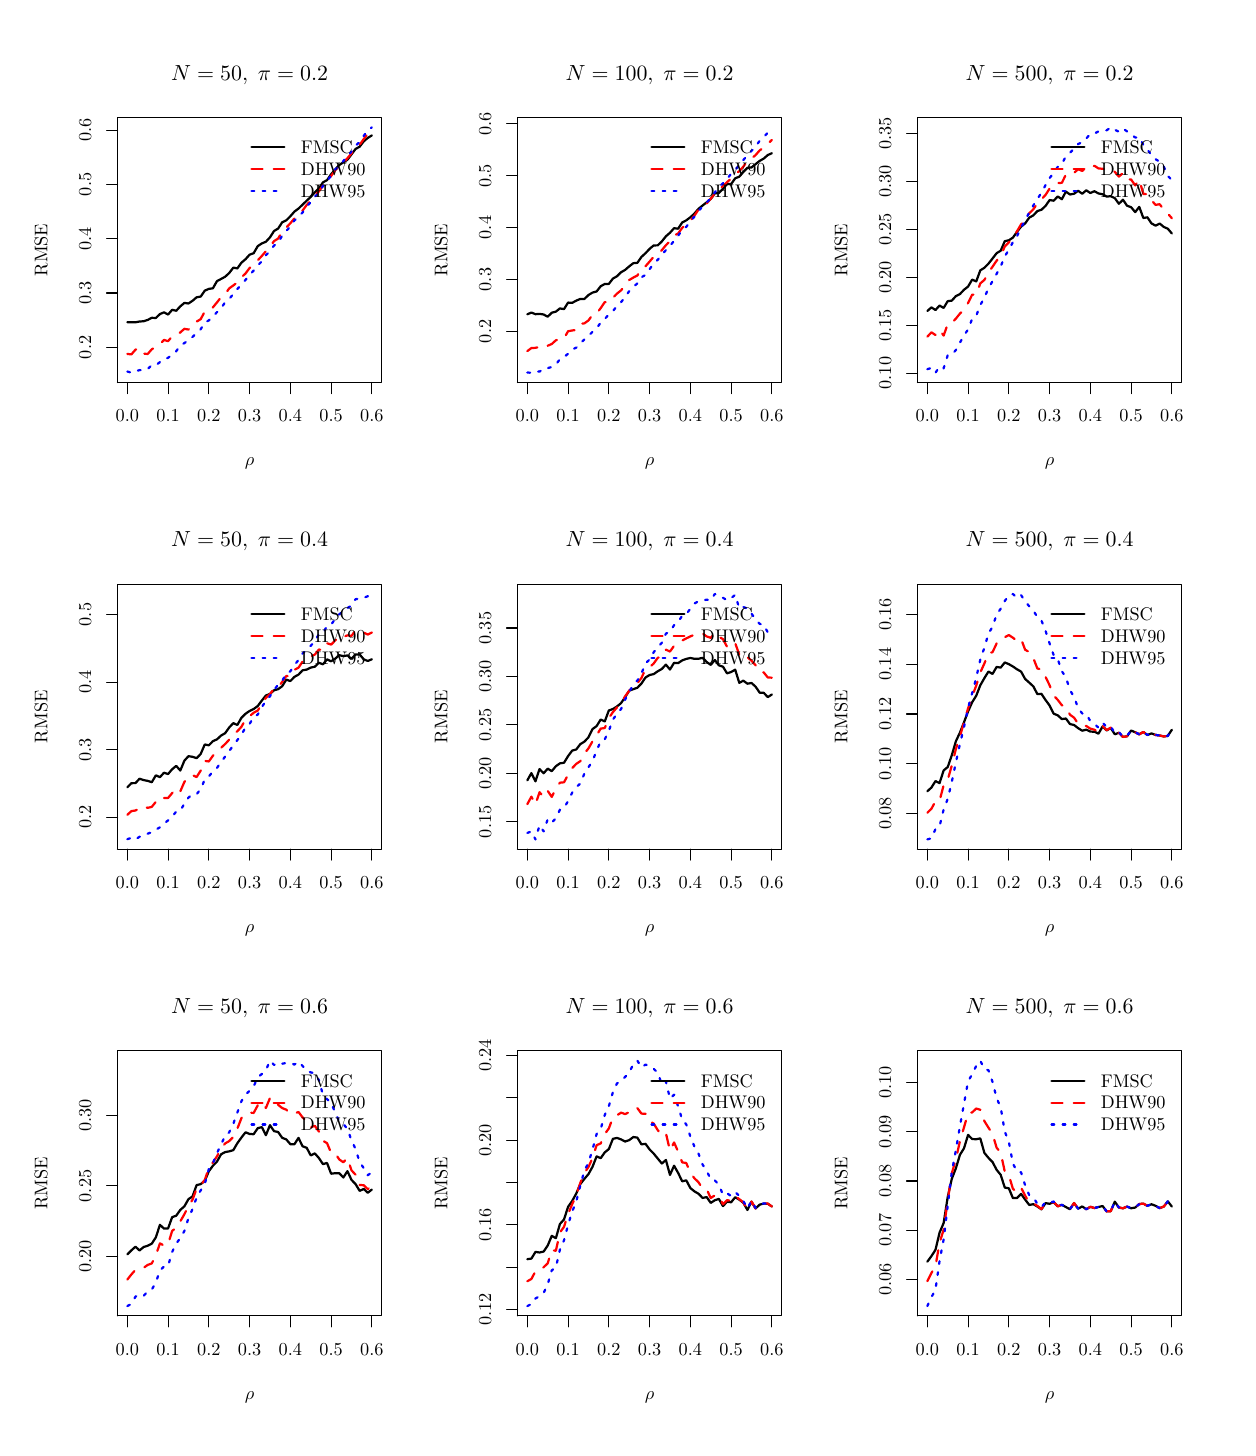
\begin{tikzpicture}[x=1pt,y=1pt]
\definecolor[named]{fillColor}{rgb}{1.00,1.00,1.00}
\path[use as bounding box,fill=fillColor,fill opacity=0.00] (0,0) rectangle (433.62,505.89);
\begin{scope}
\path[clip] ( 32.47,377.65) rectangle (127.91,473.42);
\definecolor[named]{drawColor}{rgb}{0.00,0.00,0.00}

\path[draw=drawColor,line width= 0.8pt,line join=round,line cap=round] ( 36.01,399.47) --
	( 37.48,399.47) --
	( 38.95,399.41) --
	( 40.42,399.71) --
	( 41.90,399.80) --
	( 43.37,400.28) --
	( 44.84,401.04) --
	( 46.32,400.99) --
	( 47.79,402.40) --
	( 49.26,403.03) --
	( 50.73,402.22) --
	( 52.21,403.94) --
	( 53.68,403.59) --
	( 55.15,405.19) --
	( 56.63,406.43) --
	( 58.10,406.22) --
	( 59.57,407.19) --
	( 61.04,408.46) --
	( 62.52,408.72) --
	( 63.99,410.85) --
	( 65.46,411.50) --
	( 66.93,411.71) --
	( 68.41,414.31) --
	( 69.88,415.08) --
	( 71.35,415.88) --
	( 72.83,417.24) --
	( 74.30,419.17) --
	( 75.77,418.89) --
	( 77.24,420.97) --
	( 78.72,422.22) --
	( 80.19,423.86) --
	( 81.66,424.39) --
	( 83.14,426.96) --
	( 84.61,427.92) --
	( 86.08,428.52) --
	( 87.55,430.12) --
	( 89.03,432.42) --
	( 90.50,433.29) --
	( 91.97,435.56) --
	( 93.44,436.26) --
	( 94.92,437.75) --
	( 96.39,439.42) --
	( 97.86,440.52) --
	( 99.34,441.93) --
	(100.81,443.36) --
	(102.28,444.71) --
	(103.75,446.39) --
	(105.23,447.80) --
	(106.70,450.00) --
	(108.17,450.78) --
	(109.65,452.94) --
	(111.12,454.63) --
	(112.59,456.24) --
	(114.06,457.24) --
	(115.54,458.16) --
	(117.01,460.09) --
	(118.48,462.06) --
	(119.95,462.87) --
	(121.43,464.80) --
	(122.90,466.05) --
	(124.37,466.95);
\end{scope}
\begin{scope}
\path[clip] (  0.00,  0.00) rectangle (433.62,505.89);
\definecolor[named]{drawColor}{rgb}{0.00,0.00,0.00}

\path[draw=drawColor,line width= 0.4pt,line join=round,line cap=round] ( 36.01,377.65) -- (124.37,377.65);

\path[draw=drawColor,line width= 0.4pt,line join=round,line cap=round] ( 36.01,377.65) -- ( 36.01,373.69);

\path[draw=drawColor,line width= 0.4pt,line join=round,line cap=round] ( 50.73,377.65) -- ( 50.73,373.69);

\path[draw=drawColor,line width= 0.4pt,line join=round,line cap=round] ( 65.46,377.65) -- ( 65.46,373.69);

\path[draw=drawColor,line width= 0.4pt,line join=round,line cap=round] ( 80.19,377.65) -- ( 80.19,373.69);

\path[draw=drawColor,line width= 0.4pt,line join=round,line cap=round] ( 94.92,377.65) -- ( 94.92,373.69);

\path[draw=drawColor,line width= 0.4pt,line join=round,line cap=round] (109.65,377.65) -- (109.65,373.69);

\path[draw=drawColor,line width= 0.4pt,line join=round,line cap=round] (124.37,377.65) -- (124.37,373.69);

\node[text=drawColor,anchor=base,inner sep=0pt, outer sep=0pt, scale=  0.66] at ( 36.01,363.40) {0.0};

\node[text=drawColor,anchor=base,inner sep=0pt, outer sep=0pt, scale=  0.66] at ( 50.73,363.40) {0.1};

\node[text=drawColor,anchor=base,inner sep=0pt, outer sep=0pt, scale=  0.66] at ( 65.46,363.40) {0.2};

\node[text=drawColor,anchor=base,inner sep=0pt, outer sep=0pt, scale=  0.66] at ( 80.19,363.40) {0.3};

\node[text=drawColor,anchor=base,inner sep=0pt, outer sep=0pt, scale=  0.66] at ( 94.92,363.40) {0.4};

\node[text=drawColor,anchor=base,inner sep=0pt, outer sep=0pt, scale=  0.66] at (109.65,363.40) {0.5};

\node[text=drawColor,anchor=base,inner sep=0pt, outer sep=0pt, scale=  0.66] at (124.37,363.40) {0.6};

\path[draw=drawColor,line width= 0.4pt,line join=round,line cap=round] ( 32.47,390.37) -- ( 32.47,468.88);

\path[draw=drawColor,line width= 0.4pt,line join=round,line cap=round] ( 32.47,390.37) -- ( 28.51,390.37);

\path[draw=drawColor,line width= 0.4pt,line join=round,line cap=round] ( 32.47,410.00) -- ( 28.51,410.00);

\path[draw=drawColor,line width= 0.4pt,line join=round,line cap=round] ( 32.47,429.62) -- ( 28.51,429.62);

\path[draw=drawColor,line width= 0.4pt,line join=round,line cap=round] ( 32.47,449.25) -- ( 28.51,449.25);

\path[draw=drawColor,line width= 0.4pt,line join=round,line cap=round] ( 32.47,468.88) -- ( 28.51,468.88);

\node[text=drawColor,rotate= 90.00,anchor=base,inner sep=0pt, outer sep=0pt, scale=  0.66] at ( 22.97,390.37) {0.2};

\node[text=drawColor,rotate= 90.00,anchor=base,inner sep=0pt, outer sep=0pt, scale=  0.66] at ( 22.97,410.00) {0.3};

\node[text=drawColor,rotate= 90.00,anchor=base,inner sep=0pt, outer sep=0pt, scale=  0.66] at ( 22.97,429.62) {0.4};

\node[text=drawColor,rotate= 90.00,anchor=base,inner sep=0pt, outer sep=0pt, scale=  0.66] at ( 22.97,449.25) {0.5};

\node[text=drawColor,rotate= 90.00,anchor=base,inner sep=0pt, outer sep=0pt, scale=  0.66] at ( 22.97,468.88) {0.6};

\path[draw=drawColor,line width= 0.4pt,line join=round,line cap=round] ( 32.47,377.65) --
	(127.91,377.65) --
	(127.91,473.42) --
	( 32.47,473.42) --
	( 32.47,377.65);
\end{scope}
\begin{scope}
\path[clip] (  0.00,337.26) rectangle (144.54,505.89);
\definecolor[named]{drawColor}{rgb}{0.00,0.00,0.00}

\node[text=drawColor,anchor=base,inner sep=0pt, outer sep=0pt, scale=  0.79] at ( 80.19,486.92) {\bfseries $N=50, \;\pi=0.2$};

\node[text=drawColor,anchor=base,inner sep=0pt, outer sep=0pt, scale=  0.66] at ( 80.19,347.56) {$\rho$};

\node[text=drawColor,rotate= 90.00,anchor=base,inner sep=0pt, outer sep=0pt, scale=  0.66] at (  7.13,425.53) {RMSE};
\end{scope}
\begin{scope}
\path[clip] ( 32.47,377.65) rectangle (127.91,473.42);
\definecolor[named]{drawColor}{rgb}{1.00,0.00,0.00}

\path[draw=drawColor,line width= 0.8pt,dash pattern=on 4pt off 4pt ,line join=round,line cap=round] ( 36.01,387.99) --
	( 37.48,387.83) --
	( 38.95,389.53) --
	( 40.42,390.06) --
	( 41.90,388.10) --
	( 43.37,387.97) --
	( 44.84,389.67) --
	( 46.32,390.50) --
	( 47.79,391.44) --
	( 49.26,393.07) --
	( 50.73,392.60) --
	( 52.21,394.37) --
	( 53.68,394.66) --
	( 55.15,395.77) --
	( 56.63,397.08) --
	( 58.10,396.80) --
	( 59.57,398.50) --
	( 61.04,399.68) --
	( 62.52,400.55) --
	( 63.99,403.32) --
	( 65.46,403.75) --
	( 66.93,404.82) --
	( 68.41,406.61) --
	( 69.88,408.51) --
	( 71.35,409.62) --
	( 72.83,411.69) --
	( 74.30,412.73) --
	( 75.77,413.85) --
	( 77.24,415.69) --
	( 78.72,417.06) --
	( 80.19,419.06) --
	( 81.66,420.06) --
	( 83.14,421.84) --
	( 84.61,423.39) --
	( 86.08,425.10) --
	( 87.55,426.68) --
	( 89.03,428.77) --
	( 90.50,429.68) --
	( 91.97,432.18) --
	( 93.44,433.64) --
	( 94.92,435.22) --
	( 96.39,436.96) --
	( 97.86,438.24) --
	( 99.34,439.80) --
	(100.81,441.80) --
	(102.28,443.40) --
	(103.75,445.27) --
	(105.23,446.72) --
	(106.70,448.79) --
	(108.17,450.27) --
	(109.65,452.29) --
	(111.12,454.38) --
	(112.59,455.75) --
	(114.06,457.10) --
	(115.54,458.70) --
	(117.01,460.46) --
	(118.48,462.67) --
	(119.95,463.56) --
	(121.43,465.64) --
	(122.90,467.55) --
	(124.37,468.42);
\definecolor[named]{drawColor}{rgb}{0.00,0.00,1.00}

\path[draw=drawColor,line width= 0.8pt,dash pattern=on 1pt off 3pt ,line join=round,line cap=round] ( 36.01,381.65) --
	( 37.48,381.20) --
	( 38.95,381.69) --
	( 40.42,382.15) --
	( 41.90,382.10) --
	( 43.37,382.56) --
	( 44.84,383.91) --
	( 46.32,383.88) --
	( 47.79,385.04) --
	( 49.26,386.04) --
	( 50.73,386.59) --
	( 52.21,387.72) --
	( 53.68,388.96) --
	( 55.15,391.10) --
	( 56.63,391.91) --
	( 58.10,392.95) --
	( 59.57,394.15) --
	( 61.04,395.56) --
	( 62.52,396.92) --
	( 63.99,399.31) --
	( 65.46,400.10) --
	( 66.93,401.49) --
	( 68.41,403.10) --
	( 69.88,404.49) --
	( 71.35,406.68) --
	( 72.83,407.84) --
	( 74.30,409.64) --
	( 75.77,411.46) --
	( 77.24,413.02) --
	( 78.72,414.74) --
	( 80.19,416.56) --
	( 81.66,418.11) --
	( 83.14,419.97) --
	( 84.61,421.48) --
	( 86.08,423.67) --
	( 87.55,425.15) --
	( 89.03,427.16) --
	( 90.50,428.18) --
	( 91.97,430.75) --
	( 93.44,432.41) --
	( 94.92,434.03) --
	( 96.39,436.22) --
	( 97.86,437.60) --
	( 99.34,439.08) --
	(100.81,441.24) --
	(102.28,442.83) --
	(103.75,444.80) --
	(105.23,446.18) --
	(106.70,448.66) --
	(108.17,450.46) --
	(109.65,452.40) --
	(111.12,454.59) --
	(112.59,456.17) --
	(114.06,457.68) --
	(115.54,459.45) --
	(117.01,461.12) --
	(118.48,463.24) --
	(119.95,464.57) --
	(121.43,466.80) --
	(122.90,468.74) --
	(124.37,469.87);
\definecolor[named]{drawColor}{rgb}{0.00,0.00,0.00}

\path[draw=drawColor,line width= 0.8pt,line join=round,line cap=round] ( 80.89,462.63) -- ( 92.77,462.63);
\definecolor[named]{drawColor}{rgb}{1.00,0.00,0.00}

\path[draw=drawColor,line width= 0.8pt,dash pattern=on 4pt off 4pt ,line join=round,line cap=round] ( 80.89,454.71) -- ( 92.77,454.71);
\definecolor[named]{drawColor}{rgb}{0.00,0.00,1.00}

\path[draw=drawColor,line width= 0.8pt,dash pattern=on 1pt off 3pt ,line join=round,line cap=round] ( 80.89,446.79) -- ( 92.77,446.79);
\definecolor[named]{drawColor}{rgb}{0.00,0.00,0.00}

\node[text=drawColor,anchor=base west,inner sep=0pt, outer sep=0pt, scale=  0.66] at ( 98.71,460.35) {FMSC};

\node[text=drawColor,anchor=base west,inner sep=0pt, outer sep=0pt, scale=  0.66] at ( 98.71,452.43) {DHW90};

\node[text=drawColor,anchor=base west,inner sep=0pt, outer sep=0pt, scale=  0.66] at ( 98.71,444.51) {DHW95};
\end{scope}
\begin{scope}
\path[clip] (177.01,377.65) rectangle (272.45,473.42);
\definecolor[named]{drawColor}{rgb}{0.00,0.00,0.00}

\path[draw=drawColor,line width= 0.8pt,line join=round,line cap=round] (180.55,402.31) --
	(182.02,402.94) --
	(183.49,402.35) --
	(184.96,402.47) --
	(186.44,402.24) --
	(187.91,401.44) --
	(189.38,402.89) --
	(190.86,403.28) --
	(192.33,404.44) --
	(193.80,404.18) --
	(195.27,406.55) --
	(196.75,406.44) --
	(198.22,407.25) --
	(199.69,407.86) --
	(201.17,407.85) --
	(202.64,409.28) --
	(204.11,410.16) --
	(205.58,410.57) --
	(207.06,412.45) --
	(208.53,413.28) --
	(210.00,413.30) --
	(211.47,415.21) --
	(212.95,416.07) --
	(214.42,417.51) --
	(215.89,418.36) --
	(217.37,419.64) --
	(218.84,420.78) --
	(220.31,420.91) --
	(221.78,423.04) --
	(223.26,424.40) --
	(224.73,425.97) --
	(226.20,427.19) --
	(227.68,427.23) --
	(229.15,428.64) --
	(230.62,430.50) --
	(232.09,431.77) --
	(233.57,433.43) --
	(235.04,433.24) --
	(236.51,435.50) --
	(237.98,436.26) --
	(239.46,437.37) --
	(240.93,438.72) --
	(242.40,440.44) --
	(243.88,441.62) --
	(245.35,442.77) --
	(246.82,443.98) --
	(248.29,445.98) --
	(249.77,446.13) --
	(251.24,447.68) --
	(252.71,449.35) --
	(254.19,449.38) --
	(255.66,451.45) --
	(257.13,452.04) --
	(258.60,453.74) --
	(260.08,455.26) --
	(261.55,455.37) --
	(263.02,456.57) --
	(264.50,457.74) --
	(265.97,458.58) --
	(267.44,459.86) --
	(268.91,460.52);
\end{scope}
\begin{scope}
\path[clip] (  0.00,  0.00) rectangle (433.62,505.89);
\definecolor[named]{drawColor}{rgb}{0.00,0.00,0.00}

\path[draw=drawColor,line width= 0.4pt,line join=round,line cap=round] (180.55,377.65) -- (268.91,377.65);

\path[draw=drawColor,line width= 0.4pt,line join=round,line cap=round] (180.55,377.65) -- (180.55,373.69);

\path[draw=drawColor,line width= 0.4pt,line join=round,line cap=round] (195.27,377.65) -- (195.27,373.69);

\path[draw=drawColor,line width= 0.4pt,line join=round,line cap=round] (210.00,377.65) -- (210.00,373.69);

\path[draw=drawColor,line width= 0.4pt,line join=round,line cap=round] (224.73,377.65) -- (224.73,373.69);

\path[draw=drawColor,line width= 0.4pt,line join=round,line cap=round] (239.46,377.65) -- (239.46,373.69);

\path[draw=drawColor,line width= 0.4pt,line join=round,line cap=round] (254.19,377.65) -- (254.19,373.69);

\path[draw=drawColor,line width= 0.4pt,line join=round,line cap=round] (268.91,377.65) -- (268.91,373.69);

\node[text=drawColor,anchor=base,inner sep=0pt, outer sep=0pt, scale=  0.66] at (180.55,363.40) {0.0};

\node[text=drawColor,anchor=base,inner sep=0pt, outer sep=0pt, scale=  0.66] at (195.27,363.40) {0.1};

\node[text=drawColor,anchor=base,inner sep=0pt, outer sep=0pt, scale=  0.66] at (210.00,363.40) {0.2};

\node[text=drawColor,anchor=base,inner sep=0pt, outer sep=0pt, scale=  0.66] at (224.73,363.40) {0.3};

\node[text=drawColor,anchor=base,inner sep=0pt, outer sep=0pt, scale=  0.66] at (239.46,363.40) {0.4};

\node[text=drawColor,anchor=base,inner sep=0pt, outer sep=0pt, scale=  0.66] at (254.19,363.40) {0.5};

\node[text=drawColor,anchor=base,inner sep=0pt, outer sep=0pt, scale=  0.66] at (268.91,363.40) {0.6};

\path[draw=drawColor,line width= 0.4pt,line join=round,line cap=round] (177.01,396.12) -- (177.01,471.23);

\path[draw=drawColor,line width= 0.4pt,line join=round,line cap=round] (177.01,396.12) -- (173.05,396.12);

\path[draw=drawColor,line width= 0.4pt,line join=round,line cap=round] (177.01,414.90) -- (173.05,414.90);

\path[draw=drawColor,line width= 0.4pt,line join=round,line cap=round] (177.01,433.68) -- (173.05,433.68);

\path[draw=drawColor,line width= 0.4pt,line join=round,line cap=round] (177.01,452.45) -- (173.05,452.45);

\path[draw=drawColor,line width= 0.4pt,line join=round,line cap=round] (177.01,471.23) -- (173.05,471.23);

\node[text=drawColor,rotate= 90.00,anchor=base,inner sep=0pt, outer sep=0pt, scale=  0.66] at (167.51,396.12) {0.2};

\node[text=drawColor,rotate= 90.00,anchor=base,inner sep=0pt, outer sep=0pt, scale=  0.66] at (167.51,414.90) {0.3};

\node[text=drawColor,rotate= 90.00,anchor=base,inner sep=0pt, outer sep=0pt, scale=  0.66] at (167.51,433.68) {0.4};

\node[text=drawColor,rotate= 90.00,anchor=base,inner sep=0pt, outer sep=0pt, scale=  0.66] at (167.51,452.45) {0.5};

\node[text=drawColor,rotate= 90.00,anchor=base,inner sep=0pt, outer sep=0pt, scale=  0.66] at (167.51,471.23) {0.6};

\path[draw=drawColor,line width= 0.4pt,line join=round,line cap=round] (177.01,377.65) --
	(272.45,377.65) --
	(272.45,473.42) --
	(177.01,473.42) --
	(177.01,377.65);
\end{scope}
\begin{scope}
\path[clip] (144.54,337.26) rectangle (289.08,505.89);
\definecolor[named]{drawColor}{rgb}{0.00,0.00,0.00}

\node[text=drawColor,anchor=base,inner sep=0pt, outer sep=0pt, scale=  0.79] at (224.73,486.92) {\bfseries $N=100, \;\pi=0.2$};

\node[text=drawColor,anchor=base,inner sep=0pt, outer sep=0pt, scale=  0.66] at (224.73,347.56) {$\rho$};

\node[text=drawColor,rotate= 90.00,anchor=base,inner sep=0pt, outer sep=0pt, scale=  0.66] at (151.67,425.53) {RMSE};
\end{scope}
\begin{scope}
\path[clip] (177.01,377.65) rectangle (272.45,473.42);
\definecolor[named]{drawColor}{rgb}{1.00,0.00,0.00}

\path[draw=drawColor,line width= 0.8pt,dash pattern=on 4pt off 4pt ,line join=round,line cap=round] (180.55,389.02) --
	(182.02,390.11) --
	(183.49,390.20) --
	(184.96,390.54) --
	(186.44,391.36) --
	(187.91,390.96) --
	(189.38,391.58) --
	(190.86,392.92) --
	(192.33,393.32) --
	(193.80,393.59) --
	(195.27,396.19) --
	(196.75,396.47) --
	(198.22,396.65) --
	(199.69,398.85) --
	(201.17,399.04) --
	(202.64,400.10) --
	(204.11,402.13) --
	(205.58,402.58) --
	(207.06,404.56) --
	(208.53,406.72) --
	(210.00,406.69) --
	(211.47,408.25) --
	(212.95,409.80) --
	(214.42,410.96) --
	(215.89,412.83) --
	(217.37,414.70) --
	(218.84,415.58) --
	(220.31,416.33) --
	(221.78,418.73) --
	(223.26,419.68) --
	(224.73,421.37) --
	(226.20,423.09) --
	(227.68,424.07) --
	(229.15,425.47) --
	(230.62,427.28) --
	(232.09,428.78) --
	(233.57,430.79) --
	(235.04,431.50) --
	(236.51,433.54) --
	(237.98,434.84) --
	(239.46,436.17) --
	(240.93,437.95) --
	(242.40,440.14) --
	(243.88,441.26) --
	(245.35,442.37) --
	(246.82,444.09) --
	(248.29,445.89) --
	(249.77,447.31) --
	(251.24,448.68) --
	(252.71,450.07) --
	(254.19,451.33) --
	(255.66,452.91) --
	(257.13,454.05) --
	(258.60,455.67) --
	(260.08,457.75) --
	(261.55,458.56) --
	(263.02,459.84) --
	(264.50,461.53) --
	(265.97,462.59) --
	(267.44,463.93) --
	(268.91,465.31);
\definecolor[named]{drawColor}{rgb}{0.00,0.00,1.00}

\path[draw=drawColor,line width= 0.8pt,dash pattern=on 1pt off 3pt ,line join=round,line cap=round] (180.55,381.26) --
	(182.02,381.20) --
	(183.49,381.72) --
	(184.96,381.59) --
	(186.44,382.70) --
	(187.91,382.87) --
	(189.38,383.27) --
	(190.86,384.13) --
	(192.33,386.13) --
	(193.80,386.83) --
	(195.27,388.07) --
	(196.75,389.59) --
	(198.22,390.27) --
	(199.69,391.88) --
	(201.17,393.21) --
	(202.64,394.54) --
	(204.11,395.96) --
	(205.58,397.23) --
	(207.06,399.31) --
	(208.53,400.59) --
	(210.00,402.31) --
	(211.47,403.46) --
	(212.95,405.32) --
	(214.42,406.68) --
	(215.89,408.60) --
	(217.37,410.69) --
	(218.84,412.22) --
	(220.31,413.48) --
	(221.78,415.70) --
	(223.26,416.54) --
	(224.73,418.61) --
	(226.20,420.63) --
	(227.68,422.01) --
	(229.15,423.87) --
	(230.62,425.48) --
	(232.09,427.04) --
	(233.57,428.86) --
	(235.04,430.73) --
	(236.51,432.72) --
	(237.98,433.92) --
	(239.46,435.87) --
	(240.93,437.61) --
	(242.40,439.65) --
	(243.88,441.18) --
	(245.35,442.70) --
	(246.82,444.33) --
	(248.29,446.37) --
	(249.77,448.22) --
	(251.24,449.65) --
	(252.71,451.22) --
	(254.19,453.10) --
	(255.66,454.57) --
	(257.13,456.19) --
	(258.60,458.05) --
	(260.08,459.82) --
	(261.55,461.36) --
	(263.02,462.93) --
	(264.50,465.01) --
	(265.97,466.30) --
	(267.44,467.97) --
	(268.91,469.87);
\definecolor[named]{drawColor}{rgb}{0.00,0.00,0.00}

\path[draw=drawColor,line width= 0.8pt,line join=round,line cap=round] (225.43,462.63) -- (237.31,462.63);
\definecolor[named]{drawColor}{rgb}{1.00,0.00,0.00}

\path[draw=drawColor,line width= 0.8pt,dash pattern=on 4pt off 4pt ,line join=round,line cap=round] (225.43,454.71) -- (237.31,454.71);
\definecolor[named]{drawColor}{rgb}{0.00,0.00,1.00}

\path[draw=drawColor,line width= 0.8pt,dash pattern=on 1pt off 3pt ,line join=round,line cap=round] (225.43,446.79) -- (237.31,446.79);
\definecolor[named]{drawColor}{rgb}{0.00,0.00,0.00}

\node[text=drawColor,anchor=base west,inner sep=0pt, outer sep=0pt, scale=  0.66] at (243.25,460.35) {FMSC};

\node[text=drawColor,anchor=base west,inner sep=0pt, outer sep=0pt, scale=  0.66] at (243.25,452.43) {DHW90};

\node[text=drawColor,anchor=base west,inner sep=0pt, outer sep=0pt, scale=  0.66] at (243.25,444.51) {DHW95};
\end{scope}
\begin{scope}
\path[clip] (321.55,377.65) rectangle (416.99,473.42);
\definecolor[named]{drawColor}{rgb}{0.00,0.00,0.00}

\path[draw=drawColor,line width= 0.8pt,line join=round,line cap=round] (325.09,403.51) --
	(326.56,404.81) --
	(328.03,403.86) --
	(329.50,405.48) --
	(330.98,404.61) --
	(332.45,407.06) --
	(333.92,407.25) --
	(335.40,408.88) --
	(336.87,409.63) --
	(338.34,411.18) --
	(339.81,412.34) --
	(341.29,414.85) --
	(342.76,414.20) --
	(344.23,418.20) --
	(345.71,419.12) --
	(347.18,420.62) --
	(348.65,422.48) --
	(350.12,424.39) --
	(351.60,425.29) --
	(353.07,428.74) --
	(354.54,429.06) --
	(356.01,430.03) --
	(357.49,432.10) --
	(358.96,433.99) --
	(360.43,435.15) --
	(361.91,437.24) --
	(363.38,438.05) --
	(364.85,439.62) --
	(366.32,440.09) --
	(367.80,441.47) --
	(369.27,443.60) --
	(370.74,443.36) --
	(372.22,444.89) --
	(373.69,443.89) --
	(375.16,446.65) --
	(376.63,445.61) --
	(378.11,445.87) --
	(379.58,446.95) --
	(381.05,445.87) --
	(382.52,447.12) --
	(384.00,446.14) --
	(385.47,446.79) --
	(386.94,445.97) --
	(388.42,445.69) --
	(389.89,444.85) --
	(391.36,444.99) --
	(392.83,444.29) --
	(394.31,442.25) --
	(395.78,443.71) --
	(397.25,441.55) --
	(398.73,441.01) --
	(400.20,439.23) --
	(401.67,441.12) --
	(403.14,437.11) --
	(404.62,437.36) --
	(406.09,435.16) --
	(407.56,434.34) --
	(409.04,435.11) --
	(410.51,433.89) --
	(411.98,433.24) --
	(413.45,431.52);
\end{scope}
\begin{scope}
\path[clip] (  0.00,  0.00) rectangle (433.62,505.89);
\definecolor[named]{drawColor}{rgb}{0.00,0.00,0.00}

\path[draw=drawColor,line width= 0.4pt,line join=round,line cap=round] (325.09,377.65) -- (413.45,377.65);

\path[draw=drawColor,line width= 0.4pt,line join=round,line cap=round] (325.09,377.65) -- (325.09,373.69);

\path[draw=drawColor,line width= 0.4pt,line join=round,line cap=round] (339.81,377.65) -- (339.81,373.69);

\path[draw=drawColor,line width= 0.4pt,line join=round,line cap=round] (354.54,377.65) -- (354.54,373.69);

\path[draw=drawColor,line width= 0.4pt,line join=round,line cap=round] (369.27,377.65) -- (369.27,373.69);

\path[draw=drawColor,line width= 0.4pt,line join=round,line cap=round] (384.00,377.65) -- (384.00,373.69);

\path[draw=drawColor,line width= 0.4pt,line join=round,line cap=round] (398.73,377.65) -- (398.73,373.69);

\path[draw=drawColor,line width= 0.4pt,line join=round,line cap=round] (413.45,377.65) -- (413.45,373.69);

\node[text=drawColor,anchor=base,inner sep=0pt, outer sep=0pt, scale=  0.66] at (325.09,363.40) {0.0};

\node[text=drawColor,anchor=base,inner sep=0pt, outer sep=0pt, scale=  0.66] at (339.81,363.40) {0.1};

\node[text=drawColor,anchor=base,inner sep=0pt, outer sep=0pt, scale=  0.66] at (354.54,363.40) {0.2};

\node[text=drawColor,anchor=base,inner sep=0pt, outer sep=0pt, scale=  0.66] at (369.27,363.40) {0.3};

\node[text=drawColor,anchor=base,inner sep=0pt, outer sep=0pt, scale=  0.66] at (384.00,363.40) {0.4};

\node[text=drawColor,anchor=base,inner sep=0pt, outer sep=0pt, scale=  0.66] at (398.73,363.40) {0.5};

\node[text=drawColor,anchor=base,inner sep=0pt, outer sep=0pt, scale=  0.66] at (413.45,363.40) {0.6};

\path[draw=drawColor,line width= 0.4pt,line join=round,line cap=round] (321.55,381.08) -- (321.55,467.59);

\path[draw=drawColor,line width= 0.4pt,line join=round,line cap=round] (321.55,381.08) -- (317.59,381.08);

\path[draw=drawColor,line width= 0.4pt,line join=round,line cap=round] (321.55,398.38) -- (317.59,398.38);

\path[draw=drawColor,line width= 0.4pt,line join=round,line cap=round] (321.55,415.68) -- (317.59,415.68);

\path[draw=drawColor,line width= 0.4pt,line join=round,line cap=round] (321.55,432.99) -- (317.59,432.99);

\path[draw=drawColor,line width= 0.4pt,line join=round,line cap=round] (321.55,450.29) -- (317.59,450.29);

\path[draw=drawColor,line width= 0.4pt,line join=round,line cap=round] (321.55,467.59) -- (317.59,467.59);

\node[text=drawColor,rotate= 90.00,anchor=base,inner sep=0pt, outer sep=0pt, scale=  0.66] at (312.05,381.08) {0.10};

\node[text=drawColor,rotate= 90.00,anchor=base,inner sep=0pt, outer sep=0pt, scale=  0.66] at (312.05,398.38) {0.15};

\node[text=drawColor,rotate= 90.00,anchor=base,inner sep=0pt, outer sep=0pt, scale=  0.66] at (312.05,415.68) {0.20};

\node[text=drawColor,rotate= 90.00,anchor=base,inner sep=0pt, outer sep=0pt, scale=  0.66] at (312.05,432.99) {0.25};

\node[text=drawColor,rotate= 90.00,anchor=base,inner sep=0pt, outer sep=0pt, scale=  0.66] at (312.05,450.29) {0.30};

\node[text=drawColor,rotate= 90.00,anchor=base,inner sep=0pt, outer sep=0pt, scale=  0.66] at (312.05,467.59) {0.35};

\path[draw=drawColor,line width= 0.4pt,line join=round,line cap=round] (321.55,377.65) --
	(416.99,377.65) --
	(416.99,473.42) --
	(321.55,473.42) --
	(321.55,377.65);
\end{scope}
\begin{scope}
\path[clip] (289.08,337.26) rectangle (433.62,505.89);
\definecolor[named]{drawColor}{rgb}{0.00,0.00,0.00}

\node[text=drawColor,anchor=base,inner sep=0pt, outer sep=0pt, scale=  0.79] at (369.27,486.92) {\bfseries $N=500, \;\pi=0.2$};

\node[text=drawColor,anchor=base,inner sep=0pt, outer sep=0pt, scale=  0.66] at (369.27,347.56) {$\rho$};

\node[text=drawColor,rotate= 90.00,anchor=base,inner sep=0pt, outer sep=0pt, scale=  0.66] at (296.21,425.53) {RMSE};
\end{scope}
\begin{scope}
\path[clip] (321.55,377.65) rectangle (416.99,473.42);
\definecolor[named]{drawColor}{rgb}{1.00,0.00,0.00}

\path[draw=drawColor,line width= 0.8pt,dash pattern=on 4pt off 4pt ,line join=round,line cap=round] (325.09,394.22) --
	(326.56,395.79) --
	(328.03,394.84) --
	(329.50,396.74) --
	(330.98,394.62) --
	(332.45,398.76) --
	(333.92,399.16) --
	(335.40,400.75) --
	(336.87,402.58) --
	(338.34,403.92) --
	(339.81,406.42) --
	(341.29,409.41) --
	(342.76,409.39) --
	(344.23,413.48) --
	(345.71,414.75) --
	(347.18,417.39) --
	(348.65,419.51) --
	(350.12,421.67) --
	(351.60,423.45) --
	(353.07,426.82) --
	(354.54,428.31) --
	(356.01,429.95) --
	(357.49,432.30) --
	(358.96,434.81) --
	(360.43,436.46) --
	(361.91,438.81) --
	(363.38,440.24) --
	(364.85,442.36) --
	(366.32,443.87) --
	(367.80,445.44) --
	(369.27,447.74) --
	(370.74,448.50) --
	(372.22,449.78) --
	(373.69,449.80) --
	(375.16,452.79) --
	(376.63,452.56) --
	(378.11,453.43) --
	(379.58,454.73) --
	(381.05,454.12) --
	(382.52,455.24) --
	(384.00,455.25) --
	(385.47,455.97) --
	(386.94,455.02) --
	(388.42,454.89) --
	(389.89,454.66) --
	(391.36,454.74) --
	(392.83,453.77) --
	(394.31,452.06) --
	(395.78,453.37) --
	(397.25,451.20) --
	(398.73,451.00) --
	(400.20,448.88) --
	(401.67,450.95) --
	(403.14,445.80) --
	(404.62,445.70) --
	(406.09,443.53) --
	(407.56,441.84) --
	(409.04,442.10) --
	(410.51,440.10) --
	(411.98,438.72) --
	(413.45,437.02);
\definecolor[named]{drawColor}{rgb}{0.00,0.00,1.00}

\path[draw=drawColor,line width= 0.8pt,dash pattern=on 1pt off 3pt ,line join=round,line cap=round] (325.09,382.47) --
	(326.56,382.95) --
	(328.03,381.20) --
	(329.50,383.42) --
	(330.98,382.79) --
	(332.45,387.50) --
	(333.92,387.66) --
	(335.40,389.41) --
	(336.87,392.06) --
	(338.34,394.69) --
	(339.81,396.84) --
	(341.29,400.68) --
	(342.76,401.78) --
	(344.23,405.67) --
	(345.71,408.28) --
	(347.18,411.79) --
	(348.65,414.27) --
	(350.12,416.93) --
	(351.60,419.62) --
	(353.07,423.30) --
	(354.54,425.55) --
	(356.01,428.39) --
	(357.49,430.49) --
	(358.96,433.62) --
	(360.43,436.19) --
	(361.91,439.08) --
	(363.38,441.65) --
	(364.85,443.90) --
	(366.32,446.28) --
	(367.80,448.99) --
	(369.27,451.53) --
	(370.74,453.40) --
	(372.22,455.59) --
	(373.69,456.62) --
	(375.16,459.41) --
	(376.63,460.66) --
	(378.11,462.19) --
	(379.58,463.84) --
	(381.05,464.51) --
	(382.52,465.83) --
	(384.00,467.52) --
	(385.47,467.62) --
	(386.94,468.43) --
	(388.42,468.50) --
	(389.89,468.80) --
	(391.36,469.87) --
	(392.83,468.98) --
	(394.31,468.29) --
	(395.78,469.43) --
	(397.25,468.41) --
	(398.73,467.29) --
	(400.20,466.22) --
	(401.67,466.20) --
	(403.14,463.61) --
	(404.62,461.86) --
	(406.09,459.76) --
	(407.56,458.37) --
	(409.04,457.42) --
	(410.51,455.71) --
	(411.98,452.35) --
	(413.45,450.81);
\definecolor[named]{drawColor}{rgb}{0.00,0.00,0.00}

\path[draw=drawColor,line width= 0.8pt,line join=round,line cap=round] (369.97,462.63) -- (381.85,462.63);
\definecolor[named]{drawColor}{rgb}{1.00,0.00,0.00}

\path[draw=drawColor,line width= 0.8pt,dash pattern=on 4pt off 4pt ,line join=round,line cap=round] (369.97,454.71) -- (381.85,454.71);
\definecolor[named]{drawColor}{rgb}{0.00,0.00,1.00}

\path[draw=drawColor,line width= 0.8pt,dash pattern=on 1pt off 3pt ,line join=round,line cap=round] (369.97,446.79) -- (381.85,446.79);
\definecolor[named]{drawColor}{rgb}{0.00,0.00,0.00}

\node[text=drawColor,anchor=base west,inner sep=0pt, outer sep=0pt, scale=  0.66] at (387.79,460.35) {FMSC};

\node[text=drawColor,anchor=base west,inner sep=0pt, outer sep=0pt, scale=  0.66] at (387.79,452.43) {DHW90};

\node[text=drawColor,anchor=base west,inner sep=0pt, outer sep=0pt, scale=  0.66] at (387.79,444.51) {DHW95};
\end{scope}
\begin{scope}
\path[clip] ( 32.47,209.02) rectangle (127.91,304.79);
\definecolor[named]{drawColor}{rgb}{0.00,0.00,0.00}

\path[draw=drawColor,line width= 0.8pt,line join=round,line cap=round] ( 36.01,231.39) --
	( 37.48,232.89) --
	( 38.95,232.91) --
	( 40.42,234.50) --
	( 41.90,234.01) --
	( 43.37,233.72) --
	( 44.84,233.22) --
	( 46.32,235.72) --
	( 47.79,235.06) --
	( 49.26,236.66) --
	( 50.73,236.19) --
	( 52.21,237.93) --
	( 53.68,239.14) --
	( 55.15,237.45) --
	( 56.63,241.02) --
	( 58.10,242.64) --
	( 59.57,242.42) --
	( 61.04,241.92) --
	( 62.52,243.44) --
	( 63.99,246.87) --
	( 65.46,246.56) --
	( 66.93,248.07) --
	( 68.41,248.73) --
	( 69.88,250.09) --
	( 71.35,250.94) --
	( 72.83,253.02) --
	( 74.30,254.58) --
	( 75.77,253.92) --
	( 77.24,256.52) --
	( 78.72,257.97) --
	( 80.19,258.98) --
	( 81.66,259.68) --
	( 83.14,260.77) --
	( 84.61,262.74) --
	( 86.08,264.57) --
	( 87.55,265.13) --
	( 89.03,266.46) --
	( 90.50,266.85) --
	( 91.97,267.92) --
	( 93.44,270.30) --
	( 94.92,269.78) --
	( 96.39,271.31) --
	( 97.86,272.11) --
	( 99.34,273.67) --
	(100.81,273.92) --
	(102.28,274.65) --
	(103.75,274.96) --
	(105.23,276.39) --
	(106.70,275.83) --
	(108.17,277.62) --
	(109.65,276.93) --
	(111.12,277.88) --
	(112.59,279.14) --
	(114.06,278.79) --
	(115.54,279.04) --
	(117.01,277.80) --
	(118.48,279.41) --
	(119.95,279.41) --
	(121.43,277.63) --
	(122.90,277.05) --
	(124.37,277.66);
\end{scope}
\begin{scope}
\path[clip] (  0.00,  0.00) rectangle (433.62,505.89);
\definecolor[named]{drawColor}{rgb}{0.00,0.00,0.00}

\path[draw=drawColor,line width= 0.4pt,line join=round,line cap=round] ( 36.01,209.02) -- (124.37,209.02);

\path[draw=drawColor,line width= 0.4pt,line join=round,line cap=round] ( 36.01,209.02) -- ( 36.01,205.06);

\path[draw=drawColor,line width= 0.4pt,line join=round,line cap=round] ( 50.73,209.02) -- ( 50.73,205.06);

\path[draw=drawColor,line width= 0.4pt,line join=round,line cap=round] ( 65.46,209.02) -- ( 65.46,205.06);

\path[draw=drawColor,line width= 0.4pt,line join=round,line cap=round] ( 80.19,209.02) -- ( 80.19,205.06);

\path[draw=drawColor,line width= 0.4pt,line join=round,line cap=round] ( 94.92,209.02) -- ( 94.92,205.06);

\path[draw=drawColor,line width= 0.4pt,line join=round,line cap=round] (109.65,209.02) -- (109.65,205.06);

\path[draw=drawColor,line width= 0.4pt,line join=round,line cap=round] (124.37,209.02) -- (124.37,205.06);

\node[text=drawColor,anchor=base,inner sep=0pt, outer sep=0pt, scale=  0.66] at ( 36.01,194.77) {0.0};

\node[text=drawColor,anchor=base,inner sep=0pt, outer sep=0pt, scale=  0.66] at ( 50.73,194.77) {0.1};

\node[text=drawColor,anchor=base,inner sep=0pt, outer sep=0pt, scale=  0.66] at ( 65.46,194.77) {0.2};

\node[text=drawColor,anchor=base,inner sep=0pt, outer sep=0pt, scale=  0.66] at ( 80.19,194.77) {0.3};

\node[text=drawColor,anchor=base,inner sep=0pt, outer sep=0pt, scale=  0.66] at ( 94.92,194.77) {0.4};

\node[text=drawColor,anchor=base,inner sep=0pt, outer sep=0pt, scale=  0.66] at (109.65,194.77) {0.5};

\node[text=drawColor,anchor=base,inner sep=0pt, outer sep=0pt, scale=  0.66] at (124.37,194.77) {0.6};

\path[draw=drawColor,line width= 0.4pt,line join=round,line cap=round] ( 32.47,220.56) -- ( 32.47,293.85);

\path[draw=drawColor,line width= 0.4pt,line join=round,line cap=round] ( 32.47,220.56) -- ( 28.51,220.56);

\path[draw=drawColor,line width= 0.4pt,line join=round,line cap=round] ( 32.47,244.99) -- ( 28.51,244.99);

\path[draw=drawColor,line width= 0.4pt,line join=round,line cap=round] ( 32.47,269.42) -- ( 28.51,269.42);

\path[draw=drawColor,line width= 0.4pt,line join=round,line cap=round] ( 32.47,293.85) -- ( 28.51,293.85);

\node[text=drawColor,rotate= 90.00,anchor=base,inner sep=0pt, outer sep=0pt, scale=  0.66] at ( 22.97,220.56) {0.2};

\node[text=drawColor,rotate= 90.00,anchor=base,inner sep=0pt, outer sep=0pt, scale=  0.66] at ( 22.97,244.99) {0.3};

\node[text=drawColor,rotate= 90.00,anchor=base,inner sep=0pt, outer sep=0pt, scale=  0.66] at ( 22.97,269.42) {0.4};

\node[text=drawColor,rotate= 90.00,anchor=base,inner sep=0pt, outer sep=0pt, scale=  0.66] at ( 22.97,293.85) {0.5};

\path[draw=drawColor,line width= 0.4pt,line join=round,line cap=round] ( 32.47,209.02) --
	(127.91,209.02) --
	(127.91,304.79) --
	( 32.47,304.79) --
	( 32.47,209.02);
\end{scope}
\begin{scope}
\path[clip] (  0.00,168.63) rectangle (144.54,337.26);
\definecolor[named]{drawColor}{rgb}{0.00,0.00,0.00}

\node[text=drawColor,anchor=base,inner sep=0pt, outer sep=0pt, scale=  0.79] at ( 80.19,318.29) {\bfseries $N=50, \;\pi=0.4$};

\node[text=drawColor,anchor=base,inner sep=0pt, outer sep=0pt, scale=  0.66] at ( 80.19,178.93) {$\rho$};

\node[text=drawColor,rotate= 90.00,anchor=base,inner sep=0pt, outer sep=0pt, scale=  0.66] at (  7.13,256.90) {RMSE};
\end{scope}
\begin{scope}
\path[clip] ( 32.47,209.02) rectangle (127.91,304.79);
\definecolor[named]{drawColor}{rgb}{1.00,0.00,0.00}

\path[draw=drawColor,line width= 0.8pt,dash pattern=on 4pt off 4pt ,line join=round,line cap=round] ( 36.01,221.45) --
	( 37.48,222.79) --
	( 38.95,223.02) --
	( 40.42,223.80) --
	( 41.90,224.53) --
	( 43.37,223.97) --
	( 44.84,224.32) --
	( 46.32,226.16) --
	( 47.79,225.85) --
	( 49.26,227.56) --
	( 50.73,227.54) --
	( 52.21,229.31) --
	( 53.68,231.07) --
	( 55.15,229.93) --
	( 56.63,233.35) --
	( 58.10,235.00) --
	( 59.57,235.80) --
	( 61.04,235.10) --
	( 62.52,237.43) --
	( 63.99,240.93) --
	( 65.46,240.74) --
	( 66.93,242.79) --
	( 68.41,244.11) --
	( 69.88,245.68) --
	( 71.35,247.02) --
	( 72.83,248.62) --
	( 74.30,250.73) --
	( 75.77,251.64) --
	( 77.24,253.27) --
	( 78.72,255.90) --
	( 80.19,257.06) --
	( 81.66,258.35) --
	( 83.14,259.13) --
	( 84.61,261.47) --
	( 86.08,263.73) --
	( 87.55,265.12) --
	( 89.03,267.03) --
	( 90.50,267.58) --
	( 91.97,269.48) --
	( 93.44,271.61) --
	( 94.92,271.52) --
	( 96.39,273.85) --
	( 97.86,274.61) --
	( 99.34,276.86) --
	(100.81,277.68) --
	(102.28,278.64) --
	(103.75,279.34) --
	(105.23,281.19) --
	(106.70,280.95) --
	(108.17,283.45) --
	(109.65,282.95) --
	(111.12,284.46) --
	(112.59,286.01) --
	(114.06,285.73) --
	(115.54,286.31) --
	(117.01,286.09) --
	(118.48,288.17) --
	(119.95,287.86) --
	(121.43,287.28) --
	(122.90,286.60) --
	(124.37,287.34);
\definecolor[named]{drawColor}{rgb}{0.00,0.00,1.00}

\path[draw=drawColor,line width= 0.8pt,dash pattern=on 1pt off 3pt ,line join=round,line cap=round] ( 36.01,212.65) --
	( 37.48,213.12) --
	( 38.95,212.57) --
	( 40.42,213.52) --
	( 41.90,213.86) --
	( 43.37,214.62) --
	( 44.84,215.22) --
	( 46.32,216.11) --
	( 47.79,216.93) --
	( 49.26,218.31) --
	( 50.73,219.43) --
	( 52.21,220.80) --
	( 53.68,222.63) --
	( 55.15,222.93) --
	( 56.63,225.49) --
	( 58.10,227.67) --
	( 59.57,228.90) --
	( 61.04,228.95) --
	( 62.52,230.62) --
	( 63.99,234.28) --
	( 65.46,235.34) --
	( 66.93,237.10) --
	( 68.41,238.41) --
	( 69.88,240.54) --
	( 71.35,242.50) --
	( 72.83,244.45) --
	( 74.30,246.59) --
	( 75.77,248.46) --
	( 77.24,250.39) --
	( 78.72,253.04) --
	( 80.19,254.31) --
	( 81.66,256.75) --
	( 83.14,257.67) --
	( 84.61,260.33) --
	( 86.08,262.67) --
	( 87.55,264.27) --
	( 89.03,266.63) --
	( 90.50,268.43) --
	( 91.97,269.86) --
	( 93.44,272.53) --
	( 94.92,273.30) --
	( 96.39,275.59) --
	( 97.86,277.38) --
	( 99.34,279.75) --
	(100.81,281.03) --
	(102.28,282.53) --
	(103.75,284.18) --
	(105.23,286.74) --
	(106.70,287.07) --
	(108.17,289.70) --
	(109.65,290.19) --
	(111.12,292.23) --
	(112.59,293.91) --
	(114.06,295.06) --
	(115.54,296.20) --
	(117.01,297.02) --
	(118.48,299.36) --
	(119.95,299.60) --
	(121.43,299.88) --
	(122.90,300.44) --
	(124.37,301.24);
\definecolor[named]{drawColor}{rgb}{0.00,0.00,0.00}

\path[draw=drawColor,line width= 0.8pt,line join=round,line cap=round] ( 80.89,294.00) -- ( 92.77,294.00);
\definecolor[named]{drawColor}{rgb}{1.00,0.00,0.00}

\path[draw=drawColor,line width= 0.8pt,dash pattern=on 4pt off 4pt ,line join=round,line cap=round] ( 80.89,286.08) -- ( 92.77,286.08);
\definecolor[named]{drawColor}{rgb}{0.00,0.00,1.00}

\path[draw=drawColor,line width= 0.8pt,dash pattern=on 1pt off 3pt ,line join=round,line cap=round] ( 80.89,278.16) -- ( 92.77,278.16);
\definecolor[named]{drawColor}{rgb}{0.00,0.00,0.00}

\node[text=drawColor,anchor=base west,inner sep=0pt, outer sep=0pt, scale=  0.66] at ( 98.71,291.72) {FMSC};

\node[text=drawColor,anchor=base west,inner sep=0pt, outer sep=0pt, scale=  0.66] at ( 98.71,283.80) {DHW90};

\node[text=drawColor,anchor=base west,inner sep=0pt, outer sep=0pt, scale=  0.66] at ( 98.71,275.88) {DHW95};
\end{scope}
\begin{scope}
\path[clip] (177.01,209.02) rectangle (272.45,304.79);
\definecolor[named]{drawColor}{rgb}{0.00,0.00,0.00}

\path[draw=drawColor,line width= 0.8pt,line join=round,line cap=round] (180.55,233.92) --
	(182.02,236.53) --
	(183.49,233.55) --
	(184.96,237.98) --
	(186.44,236.46) --
	(187.91,238.14) --
	(189.38,237.23) --
	(190.86,239.02) --
	(192.33,240.05) --
	(193.80,240.26) --
	(195.27,242.67) --
	(196.75,244.65) --
	(198.22,245.07) --
	(199.69,246.99) --
	(201.17,247.89) --
	(202.64,249.46) --
	(204.11,252.44) --
	(205.58,253.51) --
	(207.06,255.89) --
	(208.53,255.19) --
	(210.00,259.18) --
	(211.47,259.68) --
	(212.95,260.60) --
	(214.42,261.82) --
	(215.89,263.98) --
	(217.37,266.31) --
	(218.84,266.85) --
	(220.31,267.37) --
	(221.78,268.90) --
	(223.26,271.08) --
	(224.73,271.97) --
	(226.20,272.30) --
	(227.68,273.32) --
	(229.15,274.16) --
	(230.62,275.73) --
	(232.09,273.95) --
	(233.57,276.37) --
	(235.04,276.28) --
	(236.51,277.26) --
	(237.98,277.79) --
	(239.46,278.13) --
	(240.93,277.82) --
	(242.40,277.84) --
	(243.88,278.18) --
	(245.35,276.67) --
	(246.82,275.62) --
	(248.29,277.40) --
	(249.77,275.46) --
	(251.24,274.99) --
	(252.71,272.57) --
	(254.19,273.06) --
	(255.66,273.90) --
	(257.13,269.14) --
	(258.60,269.93) --
	(260.08,268.83) --
	(261.55,269.09) --
	(263.02,267.77) --
	(264.50,265.60) --
	(265.97,265.55) --
	(267.44,263.98) --
	(268.91,264.94);
\end{scope}
\begin{scope}
\path[clip] (  0.00,  0.00) rectangle (433.62,505.89);
\definecolor[named]{drawColor}{rgb}{0.00,0.00,0.00}

\path[draw=drawColor,line width= 0.4pt,line join=round,line cap=round] (180.55,209.02) -- (268.91,209.02);

\path[draw=drawColor,line width= 0.4pt,line join=round,line cap=round] (180.55,209.02) -- (180.55,205.06);

\path[draw=drawColor,line width= 0.4pt,line join=round,line cap=round] (195.27,209.02) -- (195.27,205.06);

\path[draw=drawColor,line width= 0.4pt,line join=round,line cap=round] (210.00,209.02) -- (210.00,205.06);

\path[draw=drawColor,line width= 0.4pt,line join=round,line cap=round] (224.73,209.02) -- (224.73,205.06);

\path[draw=drawColor,line width= 0.4pt,line join=round,line cap=round] (239.46,209.02) -- (239.46,205.06);

\path[draw=drawColor,line width= 0.4pt,line join=round,line cap=round] (254.19,209.02) -- (254.19,205.06);

\path[draw=drawColor,line width= 0.4pt,line join=round,line cap=round] (268.91,209.02) -- (268.91,205.06);

\node[text=drawColor,anchor=base,inner sep=0pt, outer sep=0pt, scale=  0.66] at (180.55,194.77) {0.0};

\node[text=drawColor,anchor=base,inner sep=0pt, outer sep=0pt, scale=  0.66] at (195.27,194.77) {0.1};

\node[text=drawColor,anchor=base,inner sep=0pt, outer sep=0pt, scale=  0.66] at (210.00,194.77) {0.2};

\node[text=drawColor,anchor=base,inner sep=0pt, outer sep=0pt, scale=  0.66] at (224.73,194.77) {0.3};

\node[text=drawColor,anchor=base,inner sep=0pt, outer sep=0pt, scale=  0.66] at (239.46,194.77) {0.4};

\node[text=drawColor,anchor=base,inner sep=0pt, outer sep=0pt, scale=  0.66] at (254.19,194.77) {0.5};

\node[text=drawColor,anchor=base,inner sep=0pt, outer sep=0pt, scale=  0.66] at (268.91,194.77) {0.6};

\path[draw=drawColor,line width= 0.4pt,line join=round,line cap=round] (177.01,218.90) -- (177.01,288.96);

\path[draw=drawColor,line width= 0.4pt,line join=round,line cap=round] (177.01,218.90) -- (173.05,218.90);

\path[draw=drawColor,line width= 0.4pt,line join=round,line cap=round] (177.01,236.42) -- (173.05,236.42);

\path[draw=drawColor,line width= 0.4pt,line join=round,line cap=round] (177.01,253.93) -- (173.05,253.93);

\path[draw=drawColor,line width= 0.4pt,line join=round,line cap=round] (177.01,271.45) -- (173.05,271.45);

\path[draw=drawColor,line width= 0.4pt,line join=round,line cap=round] (177.01,288.96) -- (173.05,288.96);

\node[text=drawColor,rotate= 90.00,anchor=base,inner sep=0pt, outer sep=0pt, scale=  0.66] at (167.51,218.90) {0.15};

\node[text=drawColor,rotate= 90.00,anchor=base,inner sep=0pt, outer sep=0pt, scale=  0.66] at (167.51,236.42) {0.20};

\node[text=drawColor,rotate= 90.00,anchor=base,inner sep=0pt, outer sep=0pt, scale=  0.66] at (167.51,253.93) {0.25};

\node[text=drawColor,rotate= 90.00,anchor=base,inner sep=0pt, outer sep=0pt, scale=  0.66] at (167.51,271.45) {0.30};

\node[text=drawColor,rotate= 90.00,anchor=base,inner sep=0pt, outer sep=0pt, scale=  0.66] at (167.51,288.96) {0.35};

\path[draw=drawColor,line width= 0.4pt,line join=round,line cap=round] (177.01,209.02) --
	(272.45,209.02) --
	(272.45,304.79) --
	(177.01,304.79) --
	(177.01,209.02);
\end{scope}
\begin{scope}
\path[clip] (144.54,168.63) rectangle (289.08,337.26);
\definecolor[named]{drawColor}{rgb}{0.00,0.00,0.00}

\node[text=drawColor,anchor=base,inner sep=0pt, outer sep=0pt, scale=  0.79] at (224.73,318.29) {\bfseries $N=100, \;\pi=0.4$};

\node[text=drawColor,anchor=base,inner sep=0pt, outer sep=0pt, scale=  0.66] at (224.73,178.93) {$\rho$};

\node[text=drawColor,rotate= 90.00,anchor=base,inner sep=0pt, outer sep=0pt, scale=  0.66] at (151.67,256.90) {RMSE};
\end{scope}
\begin{scope}
\path[clip] (177.01,209.02) rectangle (272.45,304.79);
\definecolor[named]{drawColor}{rgb}{1.00,0.00,0.00}

\path[draw=drawColor,line width= 0.8pt,dash pattern=on 4pt off 4pt ,line join=round,line cap=round] (180.55,225.30) --
	(182.02,228.03) --
	(183.49,225.20) --
	(184.96,229.62) --
	(186.44,227.88) --
	(187.91,230.09) --
	(189.38,227.92) --
	(190.86,230.98) --
	(192.33,233.07) --
	(193.80,233.20) --
	(195.27,235.90) --
	(196.75,238.34) --
	(198.22,239.85) --
	(199.69,240.83) --
	(201.17,243.60) --
	(202.64,245.46) --
	(204.11,248.01) --
	(205.58,250.19) --
	(207.06,252.61) --
	(208.53,252.81) --
	(210.00,256.42) --
	(211.47,258.56) --
	(212.95,260.27) --
	(214.42,261.61) --
	(215.89,264.29) --
	(217.37,266.28) --
	(218.84,268.37) --
	(220.31,269.04) --
	(221.78,270.88) --
	(223.26,274.15) --
	(224.73,274.80) --
	(226.20,276.11) --
	(227.68,278.19) --
	(229.15,278.64) --
	(230.62,281.15) --
	(232.09,280.44) --
	(233.57,282.51) --
	(235.04,283.25) --
	(236.51,284.42) --
	(237.98,285.21) --
	(239.46,285.94) --
	(240.93,286.50) --
	(242.40,286.63) --
	(243.88,286.95) --
	(245.35,285.92) --
	(246.82,285.40) --
	(248.29,287.14) --
	(249.77,285.81) --
	(251.24,284.92) --
	(252.71,282.19) --
	(254.19,283.54) --
	(255.66,283.53) --
	(257.13,279.30) --
	(258.60,279.87) --
	(260.08,278.41) --
	(261.55,277.16) --
	(263.02,275.50) --
	(264.50,273.10) --
	(265.97,272.91) --
	(267.44,271.07) --
	(268.91,271.01);
\definecolor[named]{drawColor}{rgb}{0.00,0.00,1.00}

\path[draw=drawColor,line width= 0.8pt,dash pattern=on 1pt off 3pt ,line join=round,line cap=round] (180.55,214.91) --
	(182.02,215.44) --
	(183.49,212.57) --
	(184.96,217.69) --
	(186.44,215.48) --
	(187.91,219.89) --
	(189.38,218.61) --
	(190.86,220.23) --
	(192.33,223.30) --
	(193.80,223.93) --
	(195.27,226.41) --
	(196.75,229.46) --
	(198.22,231.42) --
	(199.69,232.75) --
	(201.17,236.37) --
	(202.64,238.63) --
	(204.11,240.90) --
	(205.58,244.63) --
	(207.06,248.03) --
	(208.53,248.75) --
	(210.00,251.79) --
	(211.47,255.87) --
	(212.95,257.97) --
	(214.42,259.67) --
	(215.89,263.07) --
	(217.37,265.89) --
	(218.84,268.44) --
	(220.31,269.99) --
	(221.78,272.46) --
	(223.26,276.23) --
	(224.73,277.53) --
	(226.20,280.18) --
	(227.68,282.00) --
	(229.15,283.63) --
	(230.62,286.92) --
	(232.09,287.66) --
	(233.57,289.96) --
	(235.04,291.17) --
	(236.51,293.40) --
	(237.98,293.97) --
	(239.46,295.92) --
	(240.93,297.79) --
	(242.40,298.67) --
	(243.88,298.98) --
	(245.35,299.18) --
	(246.82,298.97) --
	(248.29,301.24) --
	(249.77,300.73) --
	(251.24,299.89) --
	(252.71,298.95) --
	(254.19,299.76) --
	(255.66,300.94) --
	(257.13,296.08) --
	(258.60,296.54) --
	(260.08,296.00) --
	(261.55,294.12) --
	(263.02,292.15) --
	(264.50,290.45) --
	(265.97,290.10) --
	(267.44,287.36) --
	(268.91,285.89);
\definecolor[named]{drawColor}{rgb}{0.00,0.00,0.00}

\path[draw=drawColor,line width= 0.8pt,line join=round,line cap=round] (225.43,294.00) -- (237.31,294.00);
\definecolor[named]{drawColor}{rgb}{1.00,0.00,0.00}

\path[draw=drawColor,line width= 0.8pt,dash pattern=on 4pt off 4pt ,line join=round,line cap=round] (225.43,286.08) -- (237.31,286.08);
\definecolor[named]{drawColor}{rgb}{0.00,0.00,1.00}

\path[draw=drawColor,line width= 0.8pt,dash pattern=on 1pt off 3pt ,line join=round,line cap=round] (225.43,278.16) -- (237.31,278.16);
\definecolor[named]{drawColor}{rgb}{0.00,0.00,0.00}

\node[text=drawColor,anchor=base west,inner sep=0pt, outer sep=0pt, scale=  0.66] at (243.25,291.72) {FMSC};

\node[text=drawColor,anchor=base west,inner sep=0pt, outer sep=0pt, scale=  0.66] at (243.25,283.80) {DHW90};

\node[text=drawColor,anchor=base west,inner sep=0pt, outer sep=0pt, scale=  0.66] at (243.25,275.88) {DHW95};
\end{scope}
\begin{scope}
\path[clip] (321.55,209.02) rectangle (416.99,304.79);
\definecolor[named]{drawColor}{rgb}{0.00,0.00,0.00}

\path[draw=drawColor,line width= 0.8pt,line join=round,line cap=round] (325.09,229.96) --
	(326.56,231.30) --
	(328.03,233.64) --
	(329.50,232.89) --
	(330.98,237.49) --
	(332.45,238.71) --
	(333.92,242.95) --
	(335.40,248.02) --
	(336.87,251.17) --
	(338.34,254.89) --
	(339.81,258.82) --
	(341.29,262.13) --
	(342.76,264.50) --
	(344.23,268.26) --
	(345.71,270.86) --
	(347.18,273.22) --
	(348.65,272.36) --
	(350.12,274.88) --
	(351.60,274.65) --
	(353.07,276.51) --
	(354.54,275.90) --
	(356.01,275.05) --
	(357.49,274.04) --
	(358.96,273.21) --
	(360.43,270.54) --
	(361.91,269.23) --
	(363.38,267.87) --
	(364.85,265.09) --
	(366.32,265.17) --
	(367.80,262.95) --
	(369.27,260.95) --
	(370.74,258.00) --
	(372.22,257.40) --
	(373.69,256.05) --
	(375.16,256.25) --
	(376.63,254.25) --
	(378.11,253.90) --
	(379.58,252.77) --
	(381.05,251.85) --
	(382.52,252.22) --
	(384.00,251.53) --
	(385.47,251.48) --
	(386.94,250.77) --
	(388.42,253.38) --
	(389.89,251.95) --
	(391.36,252.84) --
	(392.83,250.56) --
	(394.31,251.08) --
	(395.78,249.60) --
	(397.25,249.84) --
	(398.73,251.91) --
	(400.20,251.27) --
	(401.67,250.55) --
	(403.14,251.38) --
	(404.62,250.30) --
	(406.09,250.86) --
	(407.56,250.31) --
	(409.04,250.13) --
	(410.51,249.76) --
	(411.98,249.97) --
	(413.45,252.17);
\end{scope}
\begin{scope}
\path[clip] (  0.00,  0.00) rectangle (433.62,505.89);
\definecolor[named]{drawColor}{rgb}{0.00,0.00,0.00}

\path[draw=drawColor,line width= 0.4pt,line join=round,line cap=round] (325.09,209.02) -- (413.45,209.02);

\path[draw=drawColor,line width= 0.4pt,line join=round,line cap=round] (325.09,209.02) -- (325.09,205.06);

\path[draw=drawColor,line width= 0.4pt,line join=round,line cap=round] (339.81,209.02) -- (339.81,205.06);

\path[draw=drawColor,line width= 0.4pt,line join=round,line cap=round] (354.54,209.02) -- (354.54,205.06);

\path[draw=drawColor,line width= 0.4pt,line join=round,line cap=round] (369.27,209.02) -- (369.27,205.06);

\path[draw=drawColor,line width= 0.4pt,line join=round,line cap=round] (384.00,209.02) -- (384.00,205.06);

\path[draw=drawColor,line width= 0.4pt,line join=round,line cap=round] (398.73,209.02) -- (398.73,205.06);

\path[draw=drawColor,line width= 0.4pt,line join=round,line cap=round] (413.45,209.02) -- (413.45,205.06);

\node[text=drawColor,anchor=base,inner sep=0pt, outer sep=0pt, scale=  0.66] at (325.09,194.77) {0.0};

\node[text=drawColor,anchor=base,inner sep=0pt, outer sep=0pt, scale=  0.66] at (339.81,194.77) {0.1};

\node[text=drawColor,anchor=base,inner sep=0pt, outer sep=0pt, scale=  0.66] at (354.54,194.77) {0.2};

\node[text=drawColor,anchor=base,inner sep=0pt, outer sep=0pt, scale=  0.66] at (369.27,194.77) {0.3};

\node[text=drawColor,anchor=base,inner sep=0pt, outer sep=0pt, scale=  0.66] at (384.00,194.77) {0.4};

\node[text=drawColor,anchor=base,inner sep=0pt, outer sep=0pt, scale=  0.66] at (398.73,194.77) {0.5};

\node[text=drawColor,anchor=base,inner sep=0pt, outer sep=0pt, scale=  0.66] at (413.45,194.77) {0.6};

\path[draw=drawColor,line width= 0.4pt,line join=round,line cap=round] (321.55,221.85) -- (321.55,293.94);

\path[draw=drawColor,line width= 0.4pt,line join=round,line cap=round] (321.55,221.85) -- (317.59,221.85);

\path[draw=drawColor,line width= 0.4pt,line join=round,line cap=round] (321.55,239.87) -- (317.59,239.87);

\path[draw=drawColor,line width= 0.4pt,line join=round,line cap=round] (321.55,257.90) -- (317.59,257.90);

\path[draw=drawColor,line width= 0.4pt,line join=round,line cap=round] (321.55,275.92) -- (317.59,275.92);

\path[draw=drawColor,line width= 0.4pt,line join=round,line cap=round] (321.55,293.94) -- (317.59,293.94);

\node[text=drawColor,rotate= 90.00,anchor=base,inner sep=0pt, outer sep=0pt, scale=  0.66] at (312.05,221.85) {0.08};

\node[text=drawColor,rotate= 90.00,anchor=base,inner sep=0pt, outer sep=0pt, scale=  0.66] at (312.05,239.87) {0.10};

\node[text=drawColor,rotate= 90.00,anchor=base,inner sep=0pt, outer sep=0pt, scale=  0.66] at (312.05,257.90) {0.12};

\node[text=drawColor,rotate= 90.00,anchor=base,inner sep=0pt, outer sep=0pt, scale=  0.66] at (312.05,275.92) {0.14};

\node[text=drawColor,rotate= 90.00,anchor=base,inner sep=0pt, outer sep=0pt, scale=  0.66] at (312.05,293.94) {0.16};

\path[draw=drawColor,line width= 0.4pt,line join=round,line cap=round] (321.55,209.02) --
	(416.99,209.02) --
	(416.99,304.79) --
	(321.55,304.79) --
	(321.55,209.02);
\end{scope}
\begin{scope}
\path[clip] (289.08,168.63) rectangle (433.62,337.26);
\definecolor[named]{drawColor}{rgb}{0.00,0.00,0.00}

\node[text=drawColor,anchor=base,inner sep=0pt, outer sep=0pt, scale=  0.79] at (369.27,318.29) {\bfseries $N=500, \;\pi=0.4$};

\node[text=drawColor,anchor=base,inner sep=0pt, outer sep=0pt, scale=  0.66] at (369.27,178.93) {$\rho$};

\node[text=drawColor,rotate= 90.00,anchor=base,inner sep=0pt, outer sep=0pt, scale=  0.66] at (296.21,256.90) {RMSE};
\end{scope}
\begin{scope}
\path[clip] (321.55,209.02) rectangle (416.99,304.79);
\definecolor[named]{drawColor}{rgb}{1.00,0.00,0.00}

\path[draw=drawColor,line width= 0.8pt,dash pattern=on 4pt off 4pt ,line join=round,line cap=round] (325.09,222.21) --
	(326.56,223.63) --
	(328.03,226.36) --
	(329.50,226.51) --
	(330.98,232.15) --
	(332.45,234.10) --
	(333.92,239.23) --
	(335.40,245.22) --
	(336.87,249.76) --
	(338.34,254.87) --
	(339.81,259.92) --
	(341.29,264.28) --
	(342.76,268.15) --
	(344.23,272.88) --
	(345.71,276.17) --
	(347.18,279.81) --
	(348.65,280.22) --
	(350.12,283.37) --
	(351.60,283.97) --
	(353.07,285.63) --
	(354.54,286.41) --
	(356.01,285.45) --
	(357.49,284.30) --
	(358.96,285.00) --
	(360.43,281.11) --
	(361.91,280.25) --
	(363.38,278.11) --
	(364.85,274.32) --
	(366.32,273.99) --
	(367.80,271.30) --
	(369.27,268.26) --
	(370.74,264.55) --
	(372.22,262.98) --
	(373.69,261.06) --
	(375.16,260.47) --
	(376.63,257.63) --
	(378.11,256.55) --
	(379.58,254.35) --
	(381.05,253.48) --
	(382.52,253.54) --
	(384.00,252.59) --
	(385.47,252.20) --
	(386.94,251.35) --
	(388.42,253.60) --
	(389.89,252.04) --
	(391.36,252.97) --
	(392.83,250.56) --
	(394.31,251.12) --
	(395.78,249.60) --
	(397.25,249.84) --
	(398.73,251.91) --
	(400.20,251.27) --
	(401.67,250.55) --
	(403.14,251.38) --
	(404.62,250.30) --
	(406.09,250.86) --
	(407.56,250.31) --
	(409.04,250.13) --
	(410.51,249.76) --
	(411.98,249.97) --
	(413.45,252.17);
\definecolor[named]{drawColor}{rgb}{0.00,0.00,1.00}

\path[draw=drawColor,line width= 0.8pt,dash pattern=on 1pt off 3pt ,line join=round,line cap=round] (325.09,212.57) --
	(326.56,212.97) --
	(328.03,216.28) --
	(329.50,217.29) --
	(330.98,223.37) --
	(332.45,227.21) --
	(333.92,233.29) --
	(335.40,240.42) --
	(336.87,247.03) --
	(338.34,253.15) --
	(339.81,260.06) --
	(341.29,265.46) --
	(342.76,270.98) --
	(344.23,277.54) --
	(345.71,281.87) --
	(347.18,287.00) --
	(348.65,289.36) --
	(350.12,293.84) --
	(351.60,295.92) --
	(353.07,298.72) --
	(354.54,300.73) --
	(356.01,301.24) --
	(357.49,299.86) --
	(358.96,300.85) --
	(360.43,298.58) --
	(361.91,296.80) --
	(363.38,295.27) --
	(364.85,292.92) --
	(366.32,291.66) --
	(367.80,287.95) --
	(369.27,283.34) --
	(370.74,279.14) --
	(372.22,277.72) --
	(373.69,273.32) --
	(375.16,271.16) --
	(376.63,266.51) --
	(378.11,264.06) --
	(379.58,259.98) --
	(381.05,258.09) --
	(382.52,257.94) --
	(384.00,255.24) --
	(385.47,254.24) --
	(386.94,252.95) --
	(388.42,254.77) --
	(389.89,253.13) --
	(391.36,253.43) --
	(392.83,250.90) --
	(394.31,251.36) --
	(395.78,249.65) --
	(397.25,249.96) --
	(398.73,251.91) --
	(400.20,251.27) --
	(401.67,250.55) --
	(403.14,251.38) --
	(404.62,250.30) --
	(406.09,250.91) --
	(407.56,250.31) --
	(409.04,250.13) --
	(410.51,249.76) --
	(411.98,249.97) --
	(413.45,252.17);
\definecolor[named]{drawColor}{rgb}{0.00,0.00,0.00}

\path[draw=drawColor,line width= 0.8pt,line join=round,line cap=round] (369.97,294.00) -- (381.85,294.00);
\definecolor[named]{drawColor}{rgb}{1.00,0.00,0.00}

\path[draw=drawColor,line width= 0.8pt,dash pattern=on 4pt off 4pt ,line join=round,line cap=round] (369.97,286.08) -- (381.85,286.08);
\definecolor[named]{drawColor}{rgb}{0.00,0.00,1.00}

\path[draw=drawColor,line width= 0.8pt,dash pattern=on 1pt off 3pt ,line join=round,line cap=round] (369.97,278.16) -- (381.85,278.16);
\definecolor[named]{drawColor}{rgb}{0.00,0.00,0.00}

\node[text=drawColor,anchor=base west,inner sep=0pt, outer sep=0pt, scale=  0.66] at (387.79,291.72) {FMSC};

\node[text=drawColor,anchor=base west,inner sep=0pt, outer sep=0pt, scale=  0.66] at (387.79,283.80) {DHW90};

\node[text=drawColor,anchor=base west,inner sep=0pt, outer sep=0pt, scale=  0.66] at (387.79,275.88) {DHW95};
\end{scope}
\begin{scope}
\path[clip] ( 32.47, 40.39) rectangle (127.91,136.16);
\definecolor[named]{drawColor}{rgb}{0.00,0.00,0.00}

\path[draw=drawColor,line width= 0.8pt,line join=round,line cap=round] ( 36.01, 62.62) --
	( 37.48, 64.08) --
	( 38.95, 65.40) --
	( 40.42, 64.04) --
	( 41.90, 65.28) --
	( 43.37, 65.74) --
	( 44.84, 66.49) --
	( 46.32, 68.78) --
	( 47.79, 73.30) --
	( 49.26, 71.93) --
	( 50.73, 71.99) --
	( 52.21, 76.07) --
	( 53.68, 76.60) --
	( 55.15, 78.69) --
	( 56.63, 79.98) --
	( 58.10, 82.58) --
	( 59.57, 83.56) --
	( 61.04, 87.65) --
	( 62.52, 88.00) --
	( 63.99, 89.15) --
	( 65.46, 92.64) --
	( 66.93, 94.64) --
	( 68.41, 96.15) --
	( 69.88, 98.79) --
	( 71.35, 99.58) --
	( 72.83, 99.85) --
	( 74.30,100.28) --
	( 75.77,102.79) --
	( 77.24,104.83) --
	( 78.72,106.74) --
	( 80.19,106.13) --
	( 81.66,106.04) --
	( 83.14,108.23) --
	( 84.61,108.60) --
	( 86.08,105.68) --
	( 87.55,109.31) --
	( 89.03,107.14) --
	( 90.50,106.84) --
	( 91.97,104.73) --
	( 93.44,104.17) --
	( 94.92,102.43) --
	( 96.39,102.43) --
	( 97.86,104.71) --
	( 99.34,101.66) --
	(100.81,101.15) --
	(102.28, 98.38) --
	(103.75, 99.12) --
	(105.23, 97.44) --
	(106.70, 95.23) --
	(108.17, 95.66) --
	(109.65, 91.77) --
	(111.12, 91.95) --
	(112.59, 91.96) --
	(114.06, 90.40) --
	(115.54, 92.70) --
	(117.01, 89.54) --
	(118.48, 88.02) --
	(119.95, 85.57) --
	(121.43, 86.25) --
	(122.90, 84.89) --
	(124.37, 86.04);
\end{scope}
\begin{scope}
\path[clip] (  0.00,  0.00) rectangle (433.62,505.89);
\definecolor[named]{drawColor}{rgb}{0.00,0.00,0.00}

\path[draw=drawColor,line width= 0.4pt,line join=round,line cap=round] ( 36.01, 40.39) -- (124.37, 40.39);

\path[draw=drawColor,line width= 0.4pt,line join=round,line cap=round] ( 36.01, 40.39) -- ( 36.01, 36.43);

\path[draw=drawColor,line width= 0.4pt,line join=round,line cap=round] ( 50.73, 40.39) -- ( 50.73, 36.43);

\path[draw=drawColor,line width= 0.4pt,line join=round,line cap=round] ( 65.46, 40.39) -- ( 65.46, 36.43);

\path[draw=drawColor,line width= 0.4pt,line join=round,line cap=round] ( 80.19, 40.39) -- ( 80.19, 36.43);

\path[draw=drawColor,line width= 0.4pt,line join=round,line cap=round] ( 94.92, 40.39) -- ( 94.92, 36.43);

\path[draw=drawColor,line width= 0.4pt,line join=round,line cap=round] (109.65, 40.39) -- (109.65, 36.43);

\path[draw=drawColor,line width= 0.4pt,line join=round,line cap=round] (124.37, 40.39) -- (124.37, 36.43);

\node[text=drawColor,anchor=base,inner sep=0pt, outer sep=0pt, scale=  0.66] at ( 36.01, 26.14) {0.0};

\node[text=drawColor,anchor=base,inner sep=0pt, outer sep=0pt, scale=  0.66] at ( 50.73, 26.14) {0.1};

\node[text=drawColor,anchor=base,inner sep=0pt, outer sep=0pt, scale=  0.66] at ( 65.46, 26.14) {0.2};

\node[text=drawColor,anchor=base,inner sep=0pt, outer sep=0pt, scale=  0.66] at ( 80.19, 26.14) {0.3};

\node[text=drawColor,anchor=base,inner sep=0pt, outer sep=0pt, scale=  0.66] at ( 94.92, 26.14) {0.4};

\node[text=drawColor,anchor=base,inner sep=0pt, outer sep=0pt, scale=  0.66] at (109.65, 26.14) {0.5};

\node[text=drawColor,anchor=base,inner sep=0pt, outer sep=0pt, scale=  0.66] at (124.37, 26.14) {0.6};

\path[draw=drawColor,line width= 0.4pt,line join=round,line cap=round] ( 32.47, 61.91) -- ( 32.47,112.82);

\path[draw=drawColor,line width= 0.4pt,line join=round,line cap=round] ( 32.47, 61.91) -- ( 28.51, 61.91);

\path[draw=drawColor,line width= 0.4pt,line join=round,line cap=round] ( 32.47, 87.36) -- ( 28.51, 87.36);

\path[draw=drawColor,line width= 0.4pt,line join=round,line cap=round] ( 32.47,112.82) -- ( 28.51,112.82);

\node[text=drawColor,rotate= 90.00,anchor=base,inner sep=0pt, outer sep=0pt, scale=  0.66] at ( 22.97, 61.91) {0.20};

\node[text=drawColor,rotate= 90.00,anchor=base,inner sep=0pt, outer sep=0pt, scale=  0.66] at ( 22.97, 87.36) {0.25};

\node[text=drawColor,rotate= 90.00,anchor=base,inner sep=0pt, outer sep=0pt, scale=  0.66] at ( 22.97,112.82) {0.30};

\path[draw=drawColor,line width= 0.4pt,line join=round,line cap=round] ( 32.47, 40.39) --
	(127.91, 40.39) --
	(127.91,136.16) --
	( 32.47,136.16) --
	( 32.47, 40.39);
\end{scope}
\begin{scope}
\path[clip] (  0.00,  0.00) rectangle (144.54,168.63);
\definecolor[named]{drawColor}{rgb}{0.00,0.00,0.00}

\node[text=drawColor,anchor=base,inner sep=0pt, outer sep=0pt, scale=  0.79] at ( 80.19,149.66) {\bfseries $N=50, \;\pi=0.6$};

\node[text=drawColor,anchor=base,inner sep=0pt, outer sep=0pt, scale=  0.66] at ( 80.19, 10.30) {$\rho$};

\node[text=drawColor,rotate= 90.00,anchor=base,inner sep=0pt, outer sep=0pt, scale=  0.66] at (  7.13, 88.27) {RMSE};
\end{scope}
\begin{scope}
\path[clip] ( 32.47, 40.39) rectangle (127.91,136.16);
\definecolor[named]{drawColor}{rgb}{1.00,0.00,0.00}

\path[draw=drawColor,line width= 0.8pt,dash pattern=on 4pt off 4pt ,line join=round,line cap=round] ( 36.01, 53.52) --
	( 37.48, 55.37) --
	( 38.95, 57.03) --
	( 40.42, 57.20) --
	( 41.90, 57.75) --
	( 43.37, 58.82) --
	( 44.84, 59.34) --
	( 46.32, 62.29) --
	( 47.79, 66.61) --
	( 49.26, 65.79) --
	( 50.73, 66.30) --
	( 52.21, 71.12) --
	( 53.68, 72.20) --
	( 55.15, 74.55) --
	( 56.63, 77.13) --
	( 58.10, 80.10) --
	( 59.57, 82.38) --
	( 61.04, 86.34) --
	( 62.52, 87.74) --
	( 63.99, 89.49) --
	( 65.46, 93.77) --
	( 66.93, 95.80) --
	( 68.41, 98.07) --
	( 69.88,100.79) --
	( 71.35,102.71) --
	( 72.83,103.56) --
	( 74.30,105.04) --
	( 75.77,108.07) --
	( 77.24,111.85) --
	( 78.72,113.35) --
	( 80.19,113.78) --
	( 81.66,113.74) --
	( 83.14,116.47) --
	( 84.61,117.54) --
	( 86.08,115.51) --
	( 87.55,119.10) --
	( 89.03,117.32) --
	( 90.50,116.67) --
	( 91.97,115.49) --
	( 93.44,114.90) --
	( 94.92,113.48) --
	( 96.39,113.48) --
	( 97.86,114.07) --
	( 99.34,112.12) --
	(100.81,110.66) --
	(102.28,108.52) --
	(103.75,109.08) --
	(105.23,107.02) --
	(106.70,103.67) --
	(108.17,102.82) --
	(109.65, 99.28) --
	(111.12, 99.15) --
	(112.59, 96.91) --
	(114.06, 95.91) --
	(115.54, 97.45) --
	(117.01, 93.00) --
	(118.48, 91.40) --
	(119.95, 87.71) --
	(121.43, 87.60) --
	(122.90, 86.17) --
	(124.37, 87.56);
\definecolor[named]{drawColor}{rgb}{0.00,0.00,1.00}

\path[draw=drawColor,line width= 0.8pt,dash pattern=on 1pt off 3pt ,line join=round,line cap=round] ( 36.01, 43.94) --
	( 37.48, 44.71) --
	( 38.95, 47.36) --
	( 40.42, 48.00) --
	( 41.90, 47.63) --
	( 43.37, 49.22) --
	( 44.84, 49.90) --
	( 46.32, 52.49) --
	( 47.79, 56.86) --
	( 49.26, 58.20) --
	( 50.73, 58.43) --
	( 52.21, 63.49) --
	( 53.68, 66.55) --
	( 55.15, 68.49) --
	( 56.63, 71.07) --
	( 58.10, 75.70) --
	( 59.57, 79.01) --
	( 61.04, 83.13) --
	( 62.52, 85.74) --
	( 63.99, 88.00) --
	( 65.46, 93.45) --
	( 66.93, 95.52) --
	( 68.41, 99.21) --
	( 69.88,102.33) --
	( 71.35,105.48) --
	( 72.83,106.73) --
	( 74.30,109.79) --
	( 75.77,113.87) --
	( 77.24,117.95) --
	( 78.72,120.39) --
	( 80.19,121.71) --
	( 81.66,123.33) --
	( 83.14,126.57) --
	( 84.61,127.80) --
	( 86.08,129.17) --
	( 87.55,132.61) --
	( 89.03,131.08) --
	( 90.50,131.90) --
	( 91.97,131.51) --
	( 93.44,131.79) --
	( 94.92,131.81) --
	( 96.39,131.20) --
	( 97.86,132.27) --
	( 99.34,130.69) --
	(100.81,129.02) --
	(102.28,128.38) --
	(103.75,128.04) --
	(105.23,125.57) --
	(106.70,120.25) --
	(108.17,118.70) --
	(109.65,117.40) --
	(111.12,113.87) --
	(112.59,110.68) --
	(114.06,109.80) --
	(115.54,107.87) --
	(117.01,103.90) --
	(118.48,100.66) --
	(119.95, 96.00) --
	(121.43, 93.78) --
	(122.90, 91.24) --
	(124.37, 92.26);
\definecolor[named]{drawColor}{rgb}{0.00,0.00,0.00}

\path[draw=drawColor,line width= 0.8pt,line join=round,line cap=round] ( 80.89,125.37) -- ( 92.77,125.37);
\definecolor[named]{drawColor}{rgb}{1.00,0.00,0.00}

\path[draw=drawColor,line width= 0.8pt,dash pattern=on 4pt off 4pt ,line join=round,line cap=round] ( 80.89,117.45) -- ( 92.77,117.45);
\definecolor[named]{drawColor}{rgb}{0.00,0.00,1.00}

\path[draw=drawColor,line width= 0.8pt,dash pattern=on 1pt off 3pt ,line join=round,line cap=round] ( 80.89,109.53) -- ( 92.77,109.53);
\definecolor[named]{drawColor}{rgb}{0.00,0.00,0.00}

\node[text=drawColor,anchor=base west,inner sep=0pt, outer sep=0pt, scale=  0.66] at ( 98.71,123.09) {FMSC};

\node[text=drawColor,anchor=base west,inner sep=0pt, outer sep=0pt, scale=  0.66] at ( 98.71,115.17) {DHW90};

\node[text=drawColor,anchor=base west,inner sep=0pt, outer sep=0pt, scale=  0.66] at ( 98.71,107.25) {DHW95};
\end{scope}
\begin{scope}
\path[clip] (177.01, 40.39) rectangle (272.45,136.16);
\definecolor[named]{drawColor}{rgb}{0.00,0.00,0.00}

\path[draw=drawColor,line width= 0.8pt,line join=round,line cap=round] (180.55, 60.89) --
	(182.02, 61.09) --
	(183.49, 63.51) --
	(184.96, 63.30) --
	(186.44, 63.63) --
	(187.91, 65.81) --
	(189.38, 69.32) --
	(190.86, 68.46) --
	(192.33, 73.60) --
	(193.80, 75.23) --
	(195.27, 79.81) --
	(196.75, 81.89) --
	(198.22, 84.59) --
	(199.69, 88.02) --
	(201.17, 89.91) --
	(202.64, 91.62) --
	(204.11, 94.28) --
	(205.58, 98.04) --
	(207.06, 97.38) --
	(208.53, 99.48) --
	(210.00,100.67) --
	(211.47,104.37) --
	(212.95,104.69) --
	(214.42,104.17) --
	(215.89,103.39) --
	(217.37,103.91) --
	(218.84,105.02) --
	(220.31,104.81) --
	(221.78,102.37) --
	(223.26,102.57) --
	(224.73,100.53) --
	(226.20, 99.05) --
	(227.68, 97.24) --
	(229.15, 95.45) --
	(230.62, 96.73) --
	(232.09, 91.33) --
	(233.57, 94.66) --
	(235.04, 92.05) --
	(236.51, 89.01) --
	(237.98, 89.37) --
	(239.46, 86.59) --
	(240.93, 85.39) --
	(242.40, 84.53) --
	(243.88, 83.01) --
	(245.35, 83.32) --
	(246.82, 81.22) --
	(248.29, 82.18) --
	(249.77, 82.66) --
	(251.24, 80.06) --
	(252.71, 81.65) --
	(254.19, 81.45) --
	(255.66, 83.27) --
	(257.13, 82.40) --
	(258.60, 81.26) --
	(260.08, 78.67) --
	(261.55, 81.67) --
	(263.02, 79.20) --
	(264.50, 80.59) --
	(265.97, 80.97) --
	(267.44, 80.93) --
	(268.91, 79.92);
\end{scope}
\begin{scope}
\path[clip] (  0.00,  0.00) rectangle (433.62,505.89);
\definecolor[named]{drawColor}{rgb}{0.00,0.00,0.00}

\path[draw=drawColor,line width= 0.4pt,line join=round,line cap=round] (180.55, 40.39) -- (268.91, 40.39);

\path[draw=drawColor,line width= 0.4pt,line join=round,line cap=round] (180.55, 40.39) -- (180.55, 36.43);

\path[draw=drawColor,line width= 0.4pt,line join=round,line cap=round] (195.27, 40.39) -- (195.27, 36.43);

\path[draw=drawColor,line width= 0.4pt,line join=round,line cap=round] (210.00, 40.39) -- (210.00, 36.43);

\path[draw=drawColor,line width= 0.4pt,line join=round,line cap=round] (224.73, 40.39) -- (224.73, 36.43);

\path[draw=drawColor,line width= 0.4pt,line join=round,line cap=round] (239.46, 40.39) -- (239.46, 36.43);

\path[draw=drawColor,line width= 0.4pt,line join=round,line cap=round] (254.19, 40.39) -- (254.19, 36.43);

\path[draw=drawColor,line width= 0.4pt,line join=round,line cap=round] (268.91, 40.39) -- (268.91, 36.43);

\node[text=drawColor,anchor=base,inner sep=0pt, outer sep=0pt, scale=  0.66] at (180.55, 26.14) {0.0};

\node[text=drawColor,anchor=base,inner sep=0pt, outer sep=0pt, scale=  0.66] at (195.27, 26.14) {0.1};

\node[text=drawColor,anchor=base,inner sep=0pt, outer sep=0pt, scale=  0.66] at (210.00, 26.14) {0.2};

\node[text=drawColor,anchor=base,inner sep=0pt, outer sep=0pt, scale=  0.66] at (224.73, 26.14) {0.3};

\node[text=drawColor,anchor=base,inner sep=0pt, outer sep=0pt, scale=  0.66] at (239.46, 26.14) {0.4};

\node[text=drawColor,anchor=base,inner sep=0pt, outer sep=0pt, scale=  0.66] at (254.19, 26.14) {0.5};

\node[text=drawColor,anchor=base,inner sep=0pt, outer sep=0pt, scale=  0.66] at (268.91, 26.14) {0.6};

\path[draw=drawColor,line width= 0.4pt,line join=round,line cap=round] (177.01, 42.65) -- (177.01,134.55);

\path[draw=drawColor,line width= 0.4pt,line join=round,line cap=round] (177.01, 42.65) -- (173.05, 42.65);

\path[draw=drawColor,line width= 0.4pt,line join=round,line cap=round] (177.01, 57.97) -- (173.05, 57.97);

\path[draw=drawColor,line width= 0.4pt,line join=round,line cap=round] (177.01, 73.28) -- (173.05, 73.28);

\path[draw=drawColor,line width= 0.4pt,line join=round,line cap=round] (177.01, 88.60) -- (173.05, 88.60);

\path[draw=drawColor,line width= 0.4pt,line join=round,line cap=round] (177.01,103.91) -- (173.05,103.91);

\path[draw=drawColor,line width= 0.4pt,line join=round,line cap=round] (177.01,119.23) -- (173.05,119.23);

\path[draw=drawColor,line width= 0.4pt,line join=round,line cap=round] (177.01,134.55) -- (173.05,134.55);

\node[text=drawColor,rotate= 90.00,anchor=base,inner sep=0pt, outer sep=0pt, scale=  0.66] at (167.51, 42.65) {0.12};

\node[text=drawColor,rotate= 90.00,anchor=base,inner sep=0pt, outer sep=0pt, scale=  0.66] at (167.51, 73.28) {0.16};

\node[text=drawColor,rotate= 90.00,anchor=base,inner sep=0pt, outer sep=0pt, scale=  0.66] at (167.51,103.91) {0.20};

\node[text=drawColor,rotate= 90.00,anchor=base,inner sep=0pt, outer sep=0pt, scale=  0.66] at (167.51,134.55) {0.24};

\path[draw=drawColor,line width= 0.4pt,line join=round,line cap=round] (177.01, 40.39) --
	(272.45, 40.39) --
	(272.45,136.16) --
	(177.01,136.16) --
	(177.01, 40.39);
\end{scope}
\begin{scope}
\path[clip] (144.54,  0.00) rectangle (289.08,168.63);
\definecolor[named]{drawColor}{rgb}{0.00,0.00,0.00}

\node[text=drawColor,anchor=base,inner sep=0pt, outer sep=0pt, scale=  0.79] at (224.73,149.66) {\bfseries $N=100, \;\pi=0.6$};

\node[text=drawColor,anchor=base,inner sep=0pt, outer sep=0pt, scale=  0.66] at (224.73, 10.30) {$\rho$};

\node[text=drawColor,rotate= 90.00,anchor=base,inner sep=0pt, outer sep=0pt, scale=  0.66] at (151.67, 88.27) {RMSE};
\end{scope}
\begin{scope}
\path[clip] (177.01, 40.39) rectangle (272.45,136.16);
\definecolor[named]{drawColor}{rgb}{1.00,0.00,0.00}

\path[draw=drawColor,line width= 0.8pt,dash pattern=on 4pt off 4pt ,line join=round,line cap=round] (180.55, 52.90) --
	(182.02, 53.74) --
	(183.49, 56.52) --
	(184.96, 56.93) --
	(186.44, 57.97) --
	(187.91, 59.39) --
	(189.38, 64.17) --
	(190.86, 63.91) --
	(192.33, 70.53) --
	(193.80, 72.56) --
	(195.27, 77.18) --
	(196.75, 80.74) --
	(198.22, 83.99) --
	(199.69, 88.45) --
	(201.17, 92.06) --
	(202.64, 94.18) --
	(204.11, 97.41) --
	(205.58,102.07) --
	(207.06,102.71) --
	(208.53,106.08) --
	(210.00,108.13) --
	(211.47,112.06) --
	(212.95,112.88) --
	(214.42,113.83) --
	(215.89,113.32) --
	(217.37,114.04) --
	(218.84,115.37) --
	(220.31,115.47) --
	(221.78,113.49) --
	(223.26,113.41) --
	(224.73,110.78) --
	(226.20,109.88) --
	(227.68,107.50) --
	(229.15,105.73) --
	(230.62,106.41) --
	(232.09,100.12) --
	(233.57,103.07) --
	(235.04, 99.75) --
	(236.51, 95.86) --
	(237.98, 95.65) --
	(239.46, 92.06) --
	(240.93, 90.12) --
	(242.40, 88.67) --
	(243.88, 86.40) --
	(245.35, 86.15) --
	(246.82, 82.98) --
	(248.29, 83.93) --
	(249.77, 83.68) --
	(251.24, 80.69) --
	(252.71, 82.22) --
	(254.19, 81.96) --
	(255.66, 83.65) --
	(257.13, 82.58) --
	(258.60, 81.42) --
	(260.08, 78.72) --
	(261.55, 81.72) --
	(263.02, 79.23) --
	(264.50, 80.64) --
	(265.97, 81.02) --
	(267.44, 80.97) --
	(268.91, 79.92);
\definecolor[named]{drawColor}{rgb}{0.00,0.00,1.00}

\path[draw=drawColor,line width= 0.8pt,dash pattern=on 1pt off 3pt ,line join=round,line cap=round] (180.55, 43.94) --
	(182.02, 44.67) --
	(183.49, 46.66) --
	(184.96, 47.54) --
	(186.44, 48.70) --
	(187.91, 51.77) --
	(189.38, 56.87) --
	(190.86, 57.85) --
	(192.33, 64.38) --
	(193.80, 67.69) --
	(195.27, 73.27) --
	(196.75, 78.05) --
	(198.22, 81.69) --
	(199.69, 87.43) --
	(201.17, 92.95) --
	(202.64, 95.70) --
	(204.11,100.51) --
	(205.58,106.11) --
	(207.06,107.98) --
	(208.53,113.00) --
	(210.00,116.16) --
	(211.47,121.24) --
	(212.95,124.41) --
	(214.42,125.16) --
	(215.89,126.76) --
	(217.37,128.37) --
	(218.84,131.34) --
	(220.31,132.61) --
	(221.78,130.18) --
	(223.26,131.19) --
	(224.73,130.67) --
	(226.20,129.66) --
	(227.68,128.26) --
	(229.15,124.08) --
	(230.62,125.20) --
	(232.09,118.86) --
	(233.57,120.32) --
	(235.04,116.06) --
	(236.51,111.30) --
	(237.98,109.59) --
	(239.46,105.19) --
	(240.93,101.54) --
	(242.40, 99.02) --
	(243.88, 95.07) --
	(245.35, 92.81) --
	(246.82, 89.71) --
	(248.29, 89.37) --
	(249.77, 87.80) --
	(251.24, 84.13) --
	(252.71, 84.72) --
	(254.19, 83.69) --
	(255.66, 85.10) --
	(257.13, 83.79) --
	(258.60, 81.89) --
	(260.08, 79.22) --
	(261.55, 81.94) --
	(263.02, 79.38) --
	(264.50, 80.64) --
	(265.97, 81.02) --
	(267.44, 80.97) --
	(268.91, 79.96);
\definecolor[named]{drawColor}{rgb}{0.00,0.00,0.00}

\path[draw=drawColor,line width= 0.8pt,line join=round,line cap=round] (225.43,125.37) -- (237.31,125.37);
\definecolor[named]{drawColor}{rgb}{1.00,0.00,0.00}

\path[draw=drawColor,line width= 0.8pt,dash pattern=on 4pt off 4pt ,line join=round,line cap=round] (225.43,117.45) -- (237.31,117.45);
\definecolor[named]{drawColor}{rgb}{0.00,0.00,1.00}

\path[draw=drawColor,line width= 0.8pt,dash pattern=on 1pt off 3pt ,line join=round,line cap=round] (225.43,109.53) -- (237.31,109.53);
\definecolor[named]{drawColor}{rgb}{0.00,0.00,0.00}

\node[text=drawColor,anchor=base west,inner sep=0pt, outer sep=0pt, scale=  0.66] at (243.25,123.09) {FMSC};

\node[text=drawColor,anchor=base west,inner sep=0pt, outer sep=0pt, scale=  0.66] at (243.25,115.17) {DHW90};

\node[text=drawColor,anchor=base west,inner sep=0pt, outer sep=0pt, scale=  0.66] at (243.25,107.25) {DHW95};
\end{scope}
\begin{scope}
\path[clip] (321.55, 40.39) rectangle (416.99,136.16);
\definecolor[named]{drawColor}{rgb}{0.00,0.00,0.00}

\path[draw=drawColor,line width= 0.8pt,line join=round,line cap=round] (325.09, 59.98) --
	(326.56, 61.98) --
	(328.03, 64.25) --
	(329.50, 70.46) --
	(330.98, 73.94) --
	(332.45, 83.32) --
	(333.92, 89.90) --
	(335.40, 93.72) --
	(336.87, 98.60) --
	(338.34,100.96) --
	(339.81,105.80) --
	(341.29,104.29) --
	(342.76,104.23) --
	(344.23,104.53) --
	(345.71, 99.28) --
	(347.18, 97.48) --
	(348.65, 96.00) --
	(350.12, 93.18) --
	(351.60, 91.36) --
	(353.07, 86.75) --
	(354.54, 86.50) --
	(356.01, 82.96) --
	(357.49, 82.97) --
	(358.96, 84.47) --
	(360.43, 82.43) --
	(361.91, 80.48) --
	(363.38, 80.75) --
	(364.85, 79.93) --
	(366.32, 78.90) --
	(367.80, 81.15) --
	(369.27, 80.90) --
	(370.74, 81.48) --
	(372.22, 79.99) --
	(373.69, 80.53) --
	(375.16, 79.72) --
	(376.63, 78.93) --
	(378.11, 81.18) --
	(379.58, 79.13) --
	(381.05, 79.94) --
	(382.52, 78.94) --
	(384.00, 79.81) --
	(385.47, 79.36) --
	(386.94, 79.75) --
	(388.42, 80.08) --
	(389.89, 78.15) --
	(391.36, 78.23) --
	(392.83, 81.66) --
	(394.31, 79.55) --
	(395.78, 79.27) --
	(397.25, 79.89) --
	(398.73, 79.29) --
	(400.20, 79.54) --
	(401.67, 80.81) --
	(403.14, 80.95) --
	(404.62, 80.18) --
	(406.09, 80.73) --
	(407.56, 80.17) --
	(409.04, 79.34) --
	(410.51, 79.88) --
	(411.98, 81.77) --
	(413.45, 79.91);
\end{scope}
\begin{scope}
\path[clip] (  0.00,  0.00) rectangle (433.62,505.89);
\definecolor[named]{drawColor}{rgb}{0.00,0.00,0.00}

\path[draw=drawColor,line width= 0.4pt,line join=round,line cap=round] (325.09, 40.39) -- (413.45, 40.39);

\path[draw=drawColor,line width= 0.4pt,line join=round,line cap=round] (325.09, 40.39) -- (325.09, 36.43);

\path[draw=drawColor,line width= 0.4pt,line join=round,line cap=round] (339.81, 40.39) -- (339.81, 36.43);

\path[draw=drawColor,line width= 0.4pt,line join=round,line cap=round] (354.54, 40.39) -- (354.54, 36.43);

\path[draw=drawColor,line width= 0.4pt,line join=round,line cap=round] (369.27, 40.39) -- (369.27, 36.43);

\path[draw=drawColor,line width= 0.4pt,line join=round,line cap=round] (384.00, 40.39) -- (384.00, 36.43);

\path[draw=drawColor,line width= 0.4pt,line join=round,line cap=round] (398.73, 40.39) -- (398.73, 36.43);

\path[draw=drawColor,line width= 0.4pt,line join=round,line cap=round] (413.45, 40.39) -- (413.45, 36.43);

\node[text=drawColor,anchor=base,inner sep=0pt, outer sep=0pt, scale=  0.66] at (325.09, 26.14) {0.0};

\node[text=drawColor,anchor=base,inner sep=0pt, outer sep=0pt, scale=  0.66] at (339.81, 26.14) {0.1};

\node[text=drawColor,anchor=base,inner sep=0pt, outer sep=0pt, scale=  0.66] at (354.54, 26.14) {0.2};

\node[text=drawColor,anchor=base,inner sep=0pt, outer sep=0pt, scale=  0.66] at (369.27, 26.14) {0.3};

\node[text=drawColor,anchor=base,inner sep=0pt, outer sep=0pt, scale=  0.66] at (384.00, 26.14) {0.4};

\node[text=drawColor,anchor=base,inner sep=0pt, outer sep=0pt, scale=  0.66] at (398.73, 26.14) {0.5};

\node[text=drawColor,anchor=base,inner sep=0pt, outer sep=0pt, scale=  0.66] at (413.45, 26.14) {0.6};

\path[draw=drawColor,line width= 0.4pt,line join=round,line cap=round] (321.55, 53.66) -- (321.55,124.65);

\path[draw=drawColor,line width= 0.4pt,line join=round,line cap=round] (321.55, 53.66) -- (317.59, 53.66);

\path[draw=drawColor,line width= 0.4pt,line join=round,line cap=round] (321.55, 71.40) -- (317.59, 71.40);

\path[draw=drawColor,line width= 0.4pt,line join=round,line cap=round] (321.55, 89.15) -- (317.59, 89.15);

\path[draw=drawColor,line width= 0.4pt,line join=round,line cap=round] (321.55,106.90) -- (317.59,106.90);

\path[draw=drawColor,line width= 0.4pt,line join=round,line cap=round] (321.55,124.65) -- (317.59,124.65);

\node[text=drawColor,rotate= 90.00,anchor=base,inner sep=0pt, outer sep=0pt, scale=  0.66] at (312.05, 53.66) {0.06};

\node[text=drawColor,rotate= 90.00,anchor=base,inner sep=0pt, outer sep=0pt, scale=  0.66] at (312.05, 71.40) {0.07};

\node[text=drawColor,rotate= 90.00,anchor=base,inner sep=0pt, outer sep=0pt, scale=  0.66] at (312.05, 89.15) {0.08};

\node[text=drawColor,rotate= 90.00,anchor=base,inner sep=0pt, outer sep=0pt, scale=  0.66] at (312.05,106.90) {0.09};

\node[text=drawColor,rotate= 90.00,anchor=base,inner sep=0pt, outer sep=0pt, scale=  0.66] at (312.05,124.65) {0.10};

\path[draw=drawColor,line width= 0.4pt,line join=round,line cap=round] (321.55, 40.39) --
	(416.99, 40.39) --
	(416.99,136.16) --
	(321.55,136.16) --
	(321.55, 40.39);
\end{scope}
\begin{scope}
\path[clip] (289.08,  0.00) rectangle (433.62,168.63);
\definecolor[named]{drawColor}{rgb}{0.00,0.00,0.00}

\node[text=drawColor,anchor=base,inner sep=0pt, outer sep=0pt, scale=  0.79] at (369.27,149.66) {\bfseries $N=500, \;\pi=0.6$};

\node[text=drawColor,anchor=base,inner sep=0pt, outer sep=0pt, scale=  0.66] at (369.27, 10.30) {$\rho$};

\node[text=drawColor,rotate= 90.00,anchor=base,inner sep=0pt, outer sep=0pt, scale=  0.66] at (296.21, 88.27) {RMSE};
\end{scope}
\begin{scope}
\path[clip] (321.55, 40.39) rectangle (416.99,136.16);
\definecolor[named]{drawColor}{rgb}{1.00,0.00,0.00}

\path[draw=drawColor,line width= 0.8pt,dash pattern=on 4pt off 4pt ,line join=round,line cap=round] (325.09, 52.92) --
	(326.56, 55.89) --
	(328.03, 58.34) --
	(329.50, 66.78) --
	(330.98, 71.54) --
	(332.45, 82.04) --
	(333.92, 91.88) --
	(335.40, 96.98) --
	(336.87,103.56) --
	(338.34,108.52) --
	(339.81,113.67) --
	(341.29,113.90) --
	(342.76,115.33) --
	(344.23,114.85) --
	(345.71,110.76) --
	(347.18,108.41) --
	(348.65,106.13) --
	(350.12,101.18) --
	(351.60, 99.34) --
	(353.07, 92.53) --
	(354.54, 91.25) --
	(356.01, 86.31) --
	(357.49, 85.08) --
	(358.96, 86.73) --
	(360.43, 83.86) --
	(361.91, 81.23) --
	(363.38, 81.12) --
	(364.85, 80.12) --
	(366.32, 78.97) --
	(367.80, 81.19) --
	(369.27, 81.00) --
	(370.74, 81.54) --
	(372.22, 79.99) --
	(373.69, 80.53) --
	(375.16, 79.72) --
	(376.63, 78.93) --
	(378.11, 81.18) --
	(379.58, 79.13) --
	(381.05, 79.94) --
	(382.52, 78.94) --
	(384.00, 79.81) --
	(385.47, 79.36) --
	(386.94, 79.75) --
	(388.42, 80.08) --
	(389.89, 78.15) --
	(391.36, 78.23) --
	(392.83, 81.66) --
	(394.31, 79.55) --
	(395.78, 79.27) --
	(397.25, 79.89) --
	(398.73, 79.29) --
	(400.20, 79.54) --
	(401.67, 80.81) --
	(403.14, 80.95) --
	(404.62, 80.18) --
	(406.09, 80.73) --
	(407.56, 80.17) --
	(409.04, 79.34) --
	(410.51, 79.88) --
	(411.98, 81.77) --
	(413.45, 79.91);
\definecolor[named]{drawColor}{rgb}{0.00,0.00,1.00}

\path[draw=drawColor,line width= 0.8pt,dash pattern=on 1pt off 3pt ,line join=round,line cap=round] (325.09, 43.94) --
	(326.56, 47.13) --
	(328.03, 49.84) --
	(329.50, 60.22) --
	(330.98, 67.96) --
	(332.45, 80.09) --
	(333.92, 92.39) --
	(335.40,100.20) --
	(336.87,108.96) --
	(338.34,117.10) --
	(339.81,125.17) --
	(341.29,127.69) --
	(342.76,130.77) --
	(344.23,132.61) --
	(345.71,129.57) --
	(347.18,129.14) --
	(348.65,124.92) --
	(350.12,119.11) --
	(351.60,115.70) --
	(353.07,106.98) --
	(354.54,103.30) --
	(356.01, 95.46) --
	(357.49, 92.49) --
	(358.96, 92.29) --
	(360.43, 87.57) --
	(361.91, 84.01) --
	(363.38, 83.19) --
	(364.85, 80.91) --
	(366.32, 79.67) --
	(367.80, 81.51) --
	(369.27, 81.32) --
	(370.74, 81.72) --
	(372.22, 80.16) --
	(373.69, 80.53) --
	(375.16, 79.72) --
	(376.63, 78.93) --
	(378.11, 81.18) --
	(379.58, 79.13) --
	(381.05, 79.94) --
	(382.52, 78.94) --
	(384.00, 79.81) --
	(385.47, 79.36) --
	(386.94, 79.75) --
	(388.42, 80.08) --
	(389.89, 78.15) --
	(391.36, 78.23) --
	(392.83, 81.66) --
	(394.31, 79.55) --
	(395.78, 79.27) --
	(397.25, 79.89) --
	(398.73, 79.29) --
	(400.20, 79.54) --
	(401.67, 80.81) --
	(403.14, 80.95) --
	(404.62, 80.18) --
	(406.09, 80.73) --
	(407.56, 80.17) --
	(409.04, 79.34) --
	(410.51, 79.88) --
	(411.98, 81.77) --
	(413.45, 79.91);
\definecolor[named]{drawColor}{rgb}{0.00,0.00,0.00}

\path[draw=drawColor,line width= 0.8pt,line join=round,line cap=round] (369.97,125.37) -- (381.85,125.37);
\definecolor[named]{drawColor}{rgb}{1.00,0.00,0.00}

\path[draw=drawColor,line width= 0.8pt,dash pattern=on 4pt off 4pt ,line join=round,line cap=round] (369.97,117.45) -- (381.85,117.45);
\definecolor[named]{drawColor}{rgb}{0.00,0.00,1.00}

\path[draw=drawColor,line width= 0.8pt,dash pattern=on 1pt off 3pt ,line join=round,line cap=round] (369.97,109.53) -- (381.85,109.53);
\definecolor[named]{drawColor}{rgb}{0.00,0.00,0.00}

\node[text=drawColor,anchor=base west,inner sep=0pt, outer sep=0pt, scale=  0.66] at (387.79,123.09) {FMSC};

\node[text=drawColor,anchor=base west,inner sep=0pt, outer sep=0pt, scale=  0.66] at (387.79,115.17) {DHW90};

\node[text=drawColor,anchor=base west,inner sep=0pt, outer sep=0pt, scale=  0.66] at (387.79,107.25) {DHW95};
\end{scope}
\end{tikzpicture}

	\caption{Caption goes here.}
\end{figure}

\begin{figure}
\centering
	% Created by tikzDevice version 0.7.0 on 2014-06-29 19:22:43
% !TEX encoding = UTF-8 Unicode
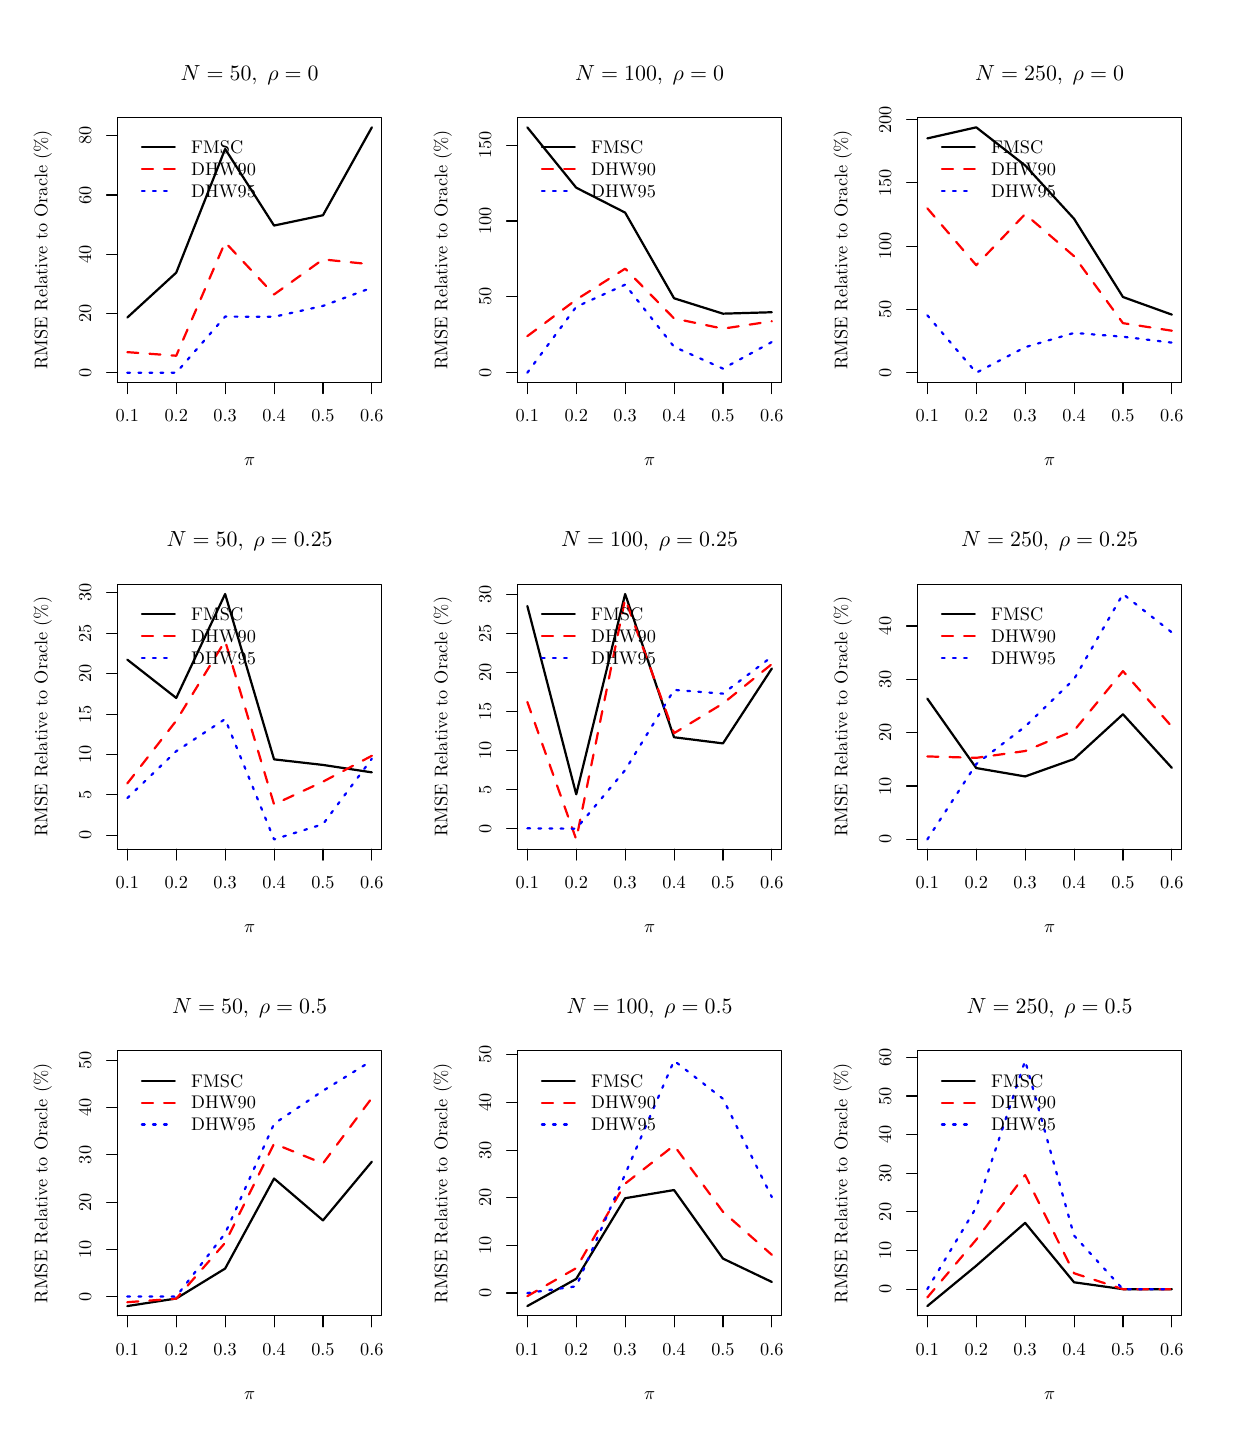
\begin{tikzpicture}[x=1pt,y=1pt]
\definecolor[named]{fillColor}{rgb}{1.00,1.00,1.00}
\path[use as bounding box,fill=fillColor,fill opacity=0.00] (0,0) rectangle (433.62,505.89);
\begin{scope}
\path[clip] ( 32.47,377.65) rectangle (127.91,473.42);
\definecolor[named]{drawColor}{rgb}{0.00,0.00,0.00}

\path[draw=drawColor,line width= 0.8pt,line join=round,line cap=round] ( 36.01,401.15) --
	( 53.68,417.36) --
	( 71.35,462.05) --
	( 89.03,434.38) --
	(106.70,438.10) --
	(124.37,469.87);
\end{scope}
\begin{scope}
\path[clip] (  0.00,  0.00) rectangle (433.62,505.89);
\definecolor[named]{drawColor}{rgb}{0.00,0.00,0.00}

\path[draw=drawColor,line width= 0.4pt,line join=round,line cap=round] ( 36.01,377.65) -- (124.37,377.65);

\path[draw=drawColor,line width= 0.4pt,line join=round,line cap=round] ( 36.01,377.65) -- ( 36.01,373.69);

\path[draw=drawColor,line width= 0.4pt,line join=round,line cap=round] ( 53.68,377.65) -- ( 53.68,373.69);

\path[draw=drawColor,line width= 0.4pt,line join=round,line cap=round] ( 71.35,377.65) -- ( 71.35,373.69);

\path[draw=drawColor,line width= 0.4pt,line join=round,line cap=round] ( 89.03,377.65) -- ( 89.03,373.69);

\path[draw=drawColor,line width= 0.4pt,line join=round,line cap=round] (106.70,377.65) -- (106.70,373.69);

\path[draw=drawColor,line width= 0.4pt,line join=round,line cap=round] (124.37,377.65) -- (124.37,373.69);

\node[text=drawColor,anchor=base,inner sep=0pt, outer sep=0pt, scale=  0.66] at ( 36.01,363.40) {0.1};

\node[text=drawColor,anchor=base,inner sep=0pt, outer sep=0pt, scale=  0.66] at ( 53.68,363.40) {0.2};

\node[text=drawColor,anchor=base,inner sep=0pt, outer sep=0pt, scale=  0.66] at ( 71.35,363.40) {0.3};

\node[text=drawColor,anchor=base,inner sep=0pt, outer sep=0pt, scale=  0.66] at ( 89.03,363.40) {0.4};

\node[text=drawColor,anchor=base,inner sep=0pt, outer sep=0pt, scale=  0.66] at (106.70,363.40) {0.5};

\node[text=drawColor,anchor=base,inner sep=0pt, outer sep=0pt, scale=  0.66] at (124.37,363.40) {0.6};

\path[draw=drawColor,line width= 0.4pt,line join=round,line cap=round] ( 32.47,381.20) -- ( 32.47,466.82);

\path[draw=drawColor,line width= 0.4pt,line join=round,line cap=round] ( 32.47,381.20) -- ( 28.51,381.20);

\path[draw=drawColor,line width= 0.4pt,line join=round,line cap=round] ( 32.47,402.61) -- ( 28.51,402.61);

\path[draw=drawColor,line width= 0.4pt,line join=round,line cap=round] ( 32.47,424.01) -- ( 28.51,424.01);

\path[draw=drawColor,line width= 0.4pt,line join=round,line cap=round] ( 32.47,445.42) -- ( 28.51,445.42);

\path[draw=drawColor,line width= 0.4pt,line join=round,line cap=round] ( 32.47,466.82) -- ( 28.51,466.82);

\node[text=drawColor,rotate= 90.00,anchor=base,inner sep=0pt, outer sep=0pt, scale=  0.66] at ( 22.97,381.20) {0};

\node[text=drawColor,rotate= 90.00,anchor=base,inner sep=0pt, outer sep=0pt, scale=  0.66] at ( 22.97,402.61) {20};

\node[text=drawColor,rotate= 90.00,anchor=base,inner sep=0pt, outer sep=0pt, scale=  0.66] at ( 22.97,424.01) {40};

\node[text=drawColor,rotate= 90.00,anchor=base,inner sep=0pt, outer sep=0pt, scale=  0.66] at ( 22.97,445.42) {60};

\node[text=drawColor,rotate= 90.00,anchor=base,inner sep=0pt, outer sep=0pt, scale=  0.66] at ( 22.97,466.82) {80};

\path[draw=drawColor,line width= 0.4pt,line join=round,line cap=round] ( 32.47,377.65) --
	(127.91,377.65) --
	(127.91,473.42) --
	( 32.47,473.42) --
	( 32.47,377.65);
\end{scope}
\begin{scope}
\path[clip] (  0.00,337.26) rectangle (144.54,505.89);
\definecolor[named]{drawColor}{rgb}{0.00,0.00,0.00}

\node[text=drawColor,anchor=base,inner sep=0pt, outer sep=0pt, scale=  0.79] at ( 80.19,486.92) {\bfseries $N=50, \;\rho=0$};

\node[text=drawColor,anchor=base,inner sep=0pt, outer sep=0pt, scale=  0.66] at ( 80.19,347.56) {$\pi$};

\node[text=drawColor,rotate= 90.00,anchor=base,inner sep=0pt, outer sep=0pt, scale=  0.66] at (  7.13,425.53) {RMSE Relative to Oracle (\%)};
\end{scope}
\begin{scope}
\path[clip] ( 32.47,377.65) rectangle (127.91,473.42);
\definecolor[named]{drawColor}{rgb}{1.00,0.00,0.00}

\path[draw=drawColor,line width= 0.8pt,dash pattern=on 4pt off 4pt ,line join=round,line cap=round] ( 36.01,388.64) --
	( 53.68,387.34) --
	( 71.35,428.32) --
	( 89.03,409.47) --
	(106.70,422.15) --
	(124.37,420.33);
\definecolor[named]{drawColor}{rgb}{0.00,0.00,1.00}

\path[draw=drawColor,line width= 0.8pt,dash pattern=on 1pt off 3pt ,line join=round,line cap=round] ( 36.01,381.20) --
	( 53.68,381.20) --
	( 71.35,401.48) --
	( 89.03,401.42) --
	(106.70,405.34) --
	(124.37,411.94);
\definecolor[named]{drawColor}{rgb}{0.00,0.00,0.00}

\path[draw=drawColor,line width= 0.8pt,line join=round,line cap=round] ( 41.28,462.63) -- ( 53.16,462.63);
\definecolor[named]{drawColor}{rgb}{1.00,0.00,0.00}

\path[draw=drawColor,line width= 0.8pt,dash pattern=on 4pt off 4pt ,line join=round,line cap=round] ( 41.28,454.71) -- ( 53.16,454.71);
\definecolor[named]{drawColor}{rgb}{0.00,0.00,1.00}

\path[draw=drawColor,line width= 0.8pt,dash pattern=on 1pt off 3pt ,line join=round,line cap=round] ( 41.28,446.79) -- ( 53.16,446.79);
\definecolor[named]{drawColor}{rgb}{0.00,0.00,0.00}

\node[text=drawColor,anchor=base west,inner sep=0pt, outer sep=0pt, scale=  0.66] at ( 59.10,460.35) {FMSC};

\node[text=drawColor,anchor=base west,inner sep=0pt, outer sep=0pt, scale=  0.66] at ( 59.10,452.43) {DHW90};

\node[text=drawColor,anchor=base west,inner sep=0pt, outer sep=0pt, scale=  0.66] at ( 59.10,444.51) {DHW95};
\end{scope}
\begin{scope}
\path[clip] (177.01,377.65) rectangle (272.45,473.42);
\definecolor[named]{drawColor}{rgb}{0.00,0.00,0.00}

\path[draw=drawColor,line width= 0.8pt,line join=round,line cap=round] (180.55,469.87) --
	(198.22,448.06) --
	(215.89,439.06) --
	(233.57,408.10) --
	(251.24,402.54) --
	(268.91,403.06);
\end{scope}
\begin{scope}
\path[clip] (  0.00,  0.00) rectangle (433.62,505.89);
\definecolor[named]{drawColor}{rgb}{0.00,0.00,0.00}

\path[draw=drawColor,line width= 0.4pt,line join=round,line cap=round] (180.55,377.65) -- (268.91,377.65);

\path[draw=drawColor,line width= 0.4pt,line join=round,line cap=round] (180.55,377.65) -- (180.55,373.69);

\path[draw=drawColor,line width= 0.4pt,line join=round,line cap=round] (198.22,377.65) -- (198.22,373.69);

\path[draw=drawColor,line width= 0.4pt,line join=round,line cap=round] (215.89,377.65) -- (215.89,373.69);

\path[draw=drawColor,line width= 0.4pt,line join=round,line cap=round] (233.57,377.65) -- (233.57,373.69);

\path[draw=drawColor,line width= 0.4pt,line join=round,line cap=round] (251.24,377.65) -- (251.24,373.69);

\path[draw=drawColor,line width= 0.4pt,line join=round,line cap=round] (268.91,377.65) -- (268.91,373.69);

\node[text=drawColor,anchor=base,inner sep=0pt, outer sep=0pt, scale=  0.66] at (180.55,363.40) {0.1};

\node[text=drawColor,anchor=base,inner sep=0pt, outer sep=0pt, scale=  0.66] at (198.22,363.40) {0.2};

\node[text=drawColor,anchor=base,inner sep=0pt, outer sep=0pt, scale=  0.66] at (215.89,363.40) {0.3};

\node[text=drawColor,anchor=base,inner sep=0pt, outer sep=0pt, scale=  0.66] at (233.57,363.40) {0.4};

\node[text=drawColor,anchor=base,inner sep=0pt, outer sep=0pt, scale=  0.66] at (251.24,363.40) {0.5};

\node[text=drawColor,anchor=base,inner sep=0pt, outer sep=0pt, scale=  0.66] at (268.91,363.40) {0.6};

\path[draw=drawColor,line width= 0.4pt,line join=round,line cap=round] (177.01,381.20) -- (177.01,463.45);

\path[draw=drawColor,line width= 0.4pt,line join=round,line cap=round] (177.01,381.20) -- (173.05,381.20);

\path[draw=drawColor,line width= 0.4pt,line join=round,line cap=round] (177.01,408.62) -- (173.05,408.62);

\path[draw=drawColor,line width= 0.4pt,line join=round,line cap=round] (177.01,436.03) -- (173.05,436.03);

\path[draw=drawColor,line width= 0.4pt,line join=round,line cap=round] (177.01,463.45) -- (173.05,463.45);

\node[text=drawColor,rotate= 90.00,anchor=base,inner sep=0pt, outer sep=0pt, scale=  0.66] at (167.51,381.20) {0};

\node[text=drawColor,rotate= 90.00,anchor=base,inner sep=0pt, outer sep=0pt, scale=  0.66] at (167.51,408.62) {50};

\node[text=drawColor,rotate= 90.00,anchor=base,inner sep=0pt, outer sep=0pt, scale=  0.66] at (167.51,436.03) {100};

\node[text=drawColor,rotate= 90.00,anchor=base,inner sep=0pt, outer sep=0pt, scale=  0.66] at (167.51,463.45) {150};

\path[draw=drawColor,line width= 0.4pt,line join=round,line cap=round] (177.01,377.65) --
	(272.45,377.65) --
	(272.45,473.42) --
	(177.01,473.42) --
	(177.01,377.65);
\end{scope}
\begin{scope}
\path[clip] (144.54,337.26) rectangle (289.08,505.89);
\definecolor[named]{drawColor}{rgb}{0.00,0.00,0.00}

\node[text=drawColor,anchor=base,inner sep=0pt, outer sep=0pt, scale=  0.79] at (224.73,486.92) {\bfseries $N=100, \;\rho=0$};

\node[text=drawColor,anchor=base,inner sep=0pt, outer sep=0pt, scale=  0.66] at (224.73,347.56) {$\pi$};

\node[text=drawColor,rotate= 90.00,anchor=base,inner sep=0pt, outer sep=0pt, scale=  0.66] at (151.67,425.53) {RMSE Relative to Oracle (\%)};
\end{scope}
\begin{scope}
\path[clip] (177.01,377.65) rectangle (272.45,473.42);
\definecolor[named]{drawColor}{rgb}{1.00,0.00,0.00}

\path[draw=drawColor,line width= 0.8pt,dash pattern=on 4pt off 4pt ,line join=round,line cap=round] (180.55,394.41) --
	(198.22,407.60) --
	(215.89,418.80) --
	(233.57,400.82) --
	(251.24,397.12) --
	(268.91,399.80);
\definecolor[named]{drawColor}{rgb}{0.00,0.00,1.00}

\path[draw=drawColor,line width= 0.8pt,dash pattern=on 1pt off 3pt ,line join=round,line cap=round] (180.55,381.20) --
	(198.22,405.02) --
	(215.89,413.03) --
	(233.57,390.56) --
	(251.24,382.69) --
	(268.91,392.30);
\definecolor[named]{drawColor}{rgb}{0.00,0.00,0.00}

\path[draw=drawColor,line width= 0.8pt,line join=round,line cap=round] (185.82,462.63) -- (197.70,462.63);
\definecolor[named]{drawColor}{rgb}{1.00,0.00,0.00}

\path[draw=drawColor,line width= 0.8pt,dash pattern=on 4pt off 4pt ,line join=round,line cap=round] (185.82,454.71) -- (197.70,454.71);
\definecolor[named]{drawColor}{rgb}{0.00,0.00,1.00}

\path[draw=drawColor,line width= 0.8pt,dash pattern=on 1pt off 3pt ,line join=round,line cap=round] (185.82,446.79) -- (197.70,446.79);
\definecolor[named]{drawColor}{rgb}{0.00,0.00,0.00}

\node[text=drawColor,anchor=base west,inner sep=0pt, outer sep=0pt, scale=  0.66] at (203.64,460.35) {FMSC};

\node[text=drawColor,anchor=base west,inner sep=0pt, outer sep=0pt, scale=  0.66] at (203.64,452.43) {DHW90};

\node[text=drawColor,anchor=base west,inner sep=0pt, outer sep=0pt, scale=  0.66] at (203.64,444.51) {DHW95};
\end{scope}
\begin{scope}
\path[clip] (321.55,377.65) rectangle (416.99,473.42);
\definecolor[named]{drawColor}{rgb}{0.00,0.00,0.00}

\path[draw=drawColor,line width= 0.8pt,line join=round,line cap=round] (325.09,465.87) --
	(342.76,469.87) --
	(360.43,456.11) --
	(378.11,436.82) --
	(395.78,408.56) --
	(413.45,402.19);
\end{scope}
\begin{scope}
\path[clip] (  0.00,  0.00) rectangle (433.62,505.89);
\definecolor[named]{drawColor}{rgb}{0.00,0.00,0.00}

\path[draw=drawColor,line width= 0.4pt,line join=round,line cap=round] (325.09,377.65) -- (413.45,377.65);

\path[draw=drawColor,line width= 0.4pt,line join=round,line cap=round] (325.09,377.65) -- (325.09,373.69);

\path[draw=drawColor,line width= 0.4pt,line join=round,line cap=round] (342.76,377.65) -- (342.76,373.69);

\path[draw=drawColor,line width= 0.4pt,line join=round,line cap=round] (360.43,377.65) -- (360.43,373.69);

\path[draw=drawColor,line width= 0.4pt,line join=round,line cap=round] (378.11,377.65) -- (378.11,373.69);

\path[draw=drawColor,line width= 0.4pt,line join=round,line cap=round] (395.78,377.65) -- (395.78,373.69);

\path[draw=drawColor,line width= 0.4pt,line join=round,line cap=round] (413.45,377.65) -- (413.45,373.69);

\node[text=drawColor,anchor=base,inner sep=0pt, outer sep=0pt, scale=  0.66] at (325.09,363.40) {0.1};

\node[text=drawColor,anchor=base,inner sep=0pt, outer sep=0pt, scale=  0.66] at (342.76,363.40) {0.2};

\node[text=drawColor,anchor=base,inner sep=0pt, outer sep=0pt, scale=  0.66] at (360.43,363.40) {0.3};

\node[text=drawColor,anchor=base,inner sep=0pt, outer sep=0pt, scale=  0.66] at (378.11,363.40) {0.4};

\node[text=drawColor,anchor=base,inner sep=0pt, outer sep=0pt, scale=  0.66] at (395.78,363.40) {0.5};

\node[text=drawColor,anchor=base,inner sep=0pt, outer sep=0pt, scale=  0.66] at (413.45,363.40) {0.6};

\path[draw=drawColor,line width= 0.4pt,line join=round,line cap=round] (321.55,381.20) -- (321.55,472.67);

\path[draw=drawColor,line width= 0.4pt,line join=round,line cap=round] (321.55,381.20) -- (317.59,381.20);

\path[draw=drawColor,line width= 0.4pt,line join=round,line cap=round] (321.55,404.07) -- (317.59,404.07);

\path[draw=drawColor,line width= 0.4pt,line join=round,line cap=round] (321.55,426.94) -- (317.59,426.94);

\path[draw=drawColor,line width= 0.4pt,line join=round,line cap=round] (321.55,449.80) -- (317.59,449.80);

\path[draw=drawColor,line width= 0.4pt,line join=round,line cap=round] (321.55,472.67) -- (317.59,472.67);

\node[text=drawColor,rotate= 90.00,anchor=base,inner sep=0pt, outer sep=0pt, scale=  0.66] at (312.05,381.20) {0};

\node[text=drawColor,rotate= 90.00,anchor=base,inner sep=0pt, outer sep=0pt, scale=  0.66] at (312.05,404.07) {50};

\node[text=drawColor,rotate= 90.00,anchor=base,inner sep=0pt, outer sep=0pt, scale=  0.66] at (312.05,426.94) {100};

\node[text=drawColor,rotate= 90.00,anchor=base,inner sep=0pt, outer sep=0pt, scale=  0.66] at (312.05,449.80) {150};

\node[text=drawColor,rotate= 90.00,anchor=base,inner sep=0pt, outer sep=0pt, scale=  0.66] at (312.05,472.67) {200};

\path[draw=drawColor,line width= 0.4pt,line join=round,line cap=round] (321.55,377.65) --
	(416.99,377.65) --
	(416.99,473.42) --
	(321.55,473.42) --
	(321.55,377.65);
\end{scope}
\begin{scope}
\path[clip] (289.08,337.26) rectangle (433.62,505.89);
\definecolor[named]{drawColor}{rgb}{0.00,0.00,0.00}

\node[text=drawColor,anchor=base,inner sep=0pt, outer sep=0pt, scale=  0.79] at (369.27,486.92) {\bfseries $N=250, \;\rho=0$};

\node[text=drawColor,anchor=base,inner sep=0pt, outer sep=0pt, scale=  0.66] at (369.27,347.56) {$\pi$};

\node[text=drawColor,rotate= 90.00,anchor=base,inner sep=0pt, outer sep=0pt, scale=  0.66] at (296.21,425.53) {RMSE Relative to Oracle (\%)};
\end{scope}
\begin{scope}
\path[clip] (321.55,377.65) rectangle (416.99,473.42);
\definecolor[named]{drawColor}{rgb}{1.00,0.00,0.00}

\path[draw=drawColor,line width= 0.8pt,dash pattern=on 4pt off 4pt ,line join=round,line cap=round] (325.09,440.61) --
	(342.76,420.05) --
	(360.43,438.52) --
	(378.11,423.30) --
	(395.78,399.11) --
	(413.45,396.38);
\definecolor[named]{drawColor}{rgb}{0.00,0.00,1.00}

\path[draw=drawColor,line width= 0.8pt,dash pattern=on 1pt off 3pt ,line join=round,line cap=round] (325.09,401.95) --
	(342.76,381.20) --
	(360.43,390.42) --
	(378.11,395.59) --
	(395.78,394.21) --
	(413.45,392.07);
\definecolor[named]{drawColor}{rgb}{0.00,0.00,0.00}

\path[draw=drawColor,line width= 0.8pt,line join=round,line cap=round] (330.36,462.63) -- (342.24,462.63);
\definecolor[named]{drawColor}{rgb}{1.00,0.00,0.00}

\path[draw=drawColor,line width= 0.8pt,dash pattern=on 4pt off 4pt ,line join=round,line cap=round] (330.36,454.71) -- (342.24,454.71);
\definecolor[named]{drawColor}{rgb}{0.00,0.00,1.00}

\path[draw=drawColor,line width= 0.8pt,dash pattern=on 1pt off 3pt ,line join=round,line cap=round] (330.36,446.79) -- (342.24,446.79);
\definecolor[named]{drawColor}{rgb}{0.00,0.00,0.00}

\node[text=drawColor,anchor=base west,inner sep=0pt, outer sep=0pt, scale=  0.66] at (348.18,460.35) {FMSC};

\node[text=drawColor,anchor=base west,inner sep=0pt, outer sep=0pt, scale=  0.66] at (348.18,452.43) {DHW90};

\node[text=drawColor,anchor=base west,inner sep=0pt, outer sep=0pt, scale=  0.66] at (348.18,444.51) {DHW95};
\end{scope}
\begin{scope}
\path[clip] ( 32.47,209.02) rectangle (127.91,304.79);
\definecolor[named]{drawColor}{rgb}{0.00,0.00,0.00}

\path[draw=drawColor,line width= 0.8pt,line join=round,line cap=round] ( 36.01,277.52) --
	( 53.68,263.68) --
	( 71.35,301.24) --
	( 89.03,241.49) --
	(106.70,239.48) --
	(124.37,236.79);
\end{scope}
\begin{scope}
\path[clip] (  0.00,  0.00) rectangle (433.62,505.89);
\definecolor[named]{drawColor}{rgb}{0.00,0.00,0.00}

\path[draw=drawColor,line width= 0.4pt,line join=round,line cap=round] ( 36.01,209.02) -- (124.37,209.02);

\path[draw=drawColor,line width= 0.4pt,line join=round,line cap=round] ( 36.01,209.02) -- ( 36.01,205.06);

\path[draw=drawColor,line width= 0.4pt,line join=round,line cap=round] ( 53.68,209.02) -- ( 53.68,205.06);

\path[draw=drawColor,line width= 0.4pt,line join=round,line cap=round] ( 71.35,209.02) -- ( 71.35,205.06);

\path[draw=drawColor,line width= 0.4pt,line join=round,line cap=round] ( 89.03,209.02) -- ( 89.03,205.06);

\path[draw=drawColor,line width= 0.4pt,line join=round,line cap=round] (106.70,209.02) -- (106.70,205.06);

\path[draw=drawColor,line width= 0.4pt,line join=round,line cap=round] (124.37,209.02) -- (124.37,205.06);

\node[text=drawColor,anchor=base,inner sep=0pt, outer sep=0pt, scale=  0.66] at ( 36.01,194.77) {0.1};

\node[text=drawColor,anchor=base,inner sep=0pt, outer sep=0pt, scale=  0.66] at ( 53.68,194.77) {0.2};

\node[text=drawColor,anchor=base,inner sep=0pt, outer sep=0pt, scale=  0.66] at ( 71.35,194.77) {0.3};

\node[text=drawColor,anchor=base,inner sep=0pt, outer sep=0pt, scale=  0.66] at ( 89.03,194.77) {0.4};

\node[text=drawColor,anchor=base,inner sep=0pt, outer sep=0pt, scale=  0.66] at (106.70,194.77) {0.5};

\node[text=drawColor,anchor=base,inner sep=0pt, outer sep=0pt, scale=  0.66] at (124.37,194.77) {0.6};

\path[draw=drawColor,line width= 0.4pt,line join=round,line cap=round] ( 32.47,214.04) -- ( 32.47,301.67);

\path[draw=drawColor,line width= 0.4pt,line join=round,line cap=round] ( 32.47,214.04) -- ( 28.51,214.04);

\path[draw=drawColor,line width= 0.4pt,line join=round,line cap=round] ( 32.47,228.65) -- ( 28.51,228.65);

\path[draw=drawColor,line width= 0.4pt,line join=round,line cap=round] ( 32.47,243.25) -- ( 28.51,243.25);

\path[draw=drawColor,line width= 0.4pt,line join=round,line cap=round] ( 32.47,257.86) -- ( 28.51,257.86);

\path[draw=drawColor,line width= 0.4pt,line join=round,line cap=round] ( 32.47,272.46) -- ( 28.51,272.46);

\path[draw=drawColor,line width= 0.4pt,line join=round,line cap=round] ( 32.47,287.07) -- ( 28.51,287.07);

\path[draw=drawColor,line width= 0.4pt,line join=round,line cap=round] ( 32.47,301.67) -- ( 28.51,301.67);

\node[text=drawColor,rotate= 90.00,anchor=base,inner sep=0pt, outer sep=0pt, scale=  0.66] at ( 22.97,214.04) {0};

\node[text=drawColor,rotate= 90.00,anchor=base,inner sep=0pt, outer sep=0pt, scale=  0.66] at ( 22.97,228.65) {5};

\node[text=drawColor,rotate= 90.00,anchor=base,inner sep=0pt, outer sep=0pt, scale=  0.66] at ( 22.97,243.25) {10};

\node[text=drawColor,rotate= 90.00,anchor=base,inner sep=0pt, outer sep=0pt, scale=  0.66] at ( 22.97,257.86) {15};

\node[text=drawColor,rotate= 90.00,anchor=base,inner sep=0pt, outer sep=0pt, scale=  0.66] at ( 22.97,272.46) {20};

\node[text=drawColor,rotate= 90.00,anchor=base,inner sep=0pt, outer sep=0pt, scale=  0.66] at ( 22.97,287.07) {25};

\node[text=drawColor,rotate= 90.00,anchor=base,inner sep=0pt, outer sep=0pt, scale=  0.66] at ( 22.97,301.67) {30};

\path[draw=drawColor,line width= 0.4pt,line join=round,line cap=round] ( 32.47,209.02) --
	(127.91,209.02) --
	(127.91,304.79) --
	( 32.47,304.79) --
	( 32.47,209.02);
\end{scope}
\begin{scope}
\path[clip] (  0.00,168.63) rectangle (144.54,337.26);
\definecolor[named]{drawColor}{rgb}{0.00,0.00,0.00}

\node[text=drawColor,anchor=base,inner sep=0pt, outer sep=0pt, scale=  0.79] at ( 80.19,318.29) {\bfseries $N=50, \;\rho=0.25$};

\node[text=drawColor,anchor=base,inner sep=0pt, outer sep=0pt, scale=  0.66] at ( 80.19,178.93) {$\pi$};

\node[text=drawColor,rotate= 90.00,anchor=base,inner sep=0pt, outer sep=0pt, scale=  0.66] at (  7.13,256.90) {RMSE Relative to Oracle (\%)};
\end{scope}
\begin{scope}
\path[clip] ( 32.47,209.02) rectangle (127.91,304.79);
\definecolor[named]{drawColor}{rgb}{1.00,0.00,0.00}

\path[draw=drawColor,line width= 0.8pt,dash pattern=on 4pt off 4pt ,line join=round,line cap=round] ( 36.01,232.79) --
	( 53.68,255.44) --
	( 71.35,284.30) --
	( 89.03,225.21) --
	(106.70,233.42) --
	(124.37,242.79);
\definecolor[named]{drawColor}{rgb}{0.00,0.00,1.00}

\path[draw=drawColor,line width= 0.8pt,dash pattern=on 1pt off 3pt ,line join=round,line cap=round] ( 36.01,227.50) --
	( 53.68,244.44) --
	( 71.35,256.05) --
	( 89.03,212.57) --
	(106.70,218.07) --
	(124.37,241.73);
\definecolor[named]{drawColor}{rgb}{0.00,0.00,0.00}

\path[draw=drawColor,line width= 0.8pt,line join=round,line cap=round] ( 41.28,294.00) -- ( 53.16,294.00);
\definecolor[named]{drawColor}{rgb}{1.00,0.00,0.00}

\path[draw=drawColor,line width= 0.8pt,dash pattern=on 4pt off 4pt ,line join=round,line cap=round] ( 41.28,286.08) -- ( 53.16,286.08);
\definecolor[named]{drawColor}{rgb}{0.00,0.00,1.00}

\path[draw=drawColor,line width= 0.8pt,dash pattern=on 1pt off 3pt ,line join=round,line cap=round] ( 41.28,278.16) -- ( 53.16,278.16);
\definecolor[named]{drawColor}{rgb}{0.00,0.00,0.00}

\node[text=drawColor,anchor=base west,inner sep=0pt, outer sep=0pt, scale=  0.66] at ( 59.10,291.72) {FMSC};

\node[text=drawColor,anchor=base west,inner sep=0pt, outer sep=0pt, scale=  0.66] at ( 59.10,283.80) {DHW90};

\node[text=drawColor,anchor=base west,inner sep=0pt, outer sep=0pt, scale=  0.66] at ( 59.10,275.88) {DHW95};
\end{scope}
\begin{scope}
\path[clip] (177.01,209.02) rectangle (272.45,304.79);
\definecolor[named]{drawColor}{rgb}{0.00,0.00,0.00}

\path[draw=drawColor,line width= 0.8pt,line join=round,line cap=round] (180.55,296.92) --
	(198.22,228.86) --
	(215.89,301.24) --
	(233.57,249.48) --
	(251.24,247.26) --
	(268.91,274.33);
\end{scope}
\begin{scope}
\path[clip] (  0.00,  0.00) rectangle (433.62,505.89);
\definecolor[named]{drawColor}{rgb}{0.00,0.00,0.00}

\path[draw=drawColor,line width= 0.4pt,line join=round,line cap=round] (180.55,209.02) -- (268.91,209.02);

\path[draw=drawColor,line width= 0.4pt,line join=round,line cap=round] (180.55,209.02) -- (180.55,205.06);

\path[draw=drawColor,line width= 0.4pt,line join=round,line cap=round] (198.22,209.02) -- (198.22,205.06);

\path[draw=drawColor,line width= 0.4pt,line join=round,line cap=round] (215.89,209.02) -- (215.89,205.06);

\path[draw=drawColor,line width= 0.4pt,line join=round,line cap=round] (233.57,209.02) -- (233.57,205.06);

\path[draw=drawColor,line width= 0.4pt,line join=round,line cap=round] (251.24,209.02) -- (251.24,205.06);

\path[draw=drawColor,line width= 0.4pt,line join=round,line cap=round] (268.91,209.02) -- (268.91,205.06);

\node[text=drawColor,anchor=base,inner sep=0pt, outer sep=0pt, scale=  0.66] at (180.55,194.77) {0.1};

\node[text=drawColor,anchor=base,inner sep=0pt, outer sep=0pt, scale=  0.66] at (198.22,194.77) {0.2};

\node[text=drawColor,anchor=base,inner sep=0pt, outer sep=0pt, scale=  0.66] at (215.89,194.77) {0.3};

\node[text=drawColor,anchor=base,inner sep=0pt, outer sep=0pt, scale=  0.66] at (233.57,194.77) {0.4};

\node[text=drawColor,anchor=base,inner sep=0pt, outer sep=0pt, scale=  0.66] at (251.24,194.77) {0.5};

\node[text=drawColor,anchor=base,inner sep=0pt, outer sep=0pt, scale=  0.66] at (268.91,194.77) {0.6};

\path[draw=drawColor,line width= 0.4pt,line join=round,line cap=round] (177.01,216.42) -- (177.01,300.97);

\path[draw=drawColor,line width= 0.4pt,line join=round,line cap=round] (177.01,216.42) -- (173.05,216.42);

\path[draw=drawColor,line width= 0.4pt,line join=round,line cap=round] (177.01,230.51) -- (173.05,230.51);

\path[draw=drawColor,line width= 0.4pt,line join=round,line cap=round] (177.01,244.61) -- (173.05,244.61);

\path[draw=drawColor,line width= 0.4pt,line join=round,line cap=round] (177.01,258.70) -- (173.05,258.70);

\path[draw=drawColor,line width= 0.4pt,line join=round,line cap=round] (177.01,272.79) -- (173.05,272.79);

\path[draw=drawColor,line width= 0.4pt,line join=round,line cap=round] (177.01,286.88) -- (173.05,286.88);

\path[draw=drawColor,line width= 0.4pt,line join=round,line cap=round] (177.01,300.97) -- (173.05,300.97);

\node[text=drawColor,rotate= 90.00,anchor=base,inner sep=0pt, outer sep=0pt, scale=  0.66] at (167.51,216.42) {0};

\node[text=drawColor,rotate= 90.00,anchor=base,inner sep=0pt, outer sep=0pt, scale=  0.66] at (167.51,230.51) {5};

\node[text=drawColor,rotate= 90.00,anchor=base,inner sep=0pt, outer sep=0pt, scale=  0.66] at (167.51,244.61) {10};

\node[text=drawColor,rotate= 90.00,anchor=base,inner sep=0pt, outer sep=0pt, scale=  0.66] at (167.51,258.70) {15};

\node[text=drawColor,rotate= 90.00,anchor=base,inner sep=0pt, outer sep=0pt, scale=  0.66] at (167.51,272.79) {20};

\node[text=drawColor,rotate= 90.00,anchor=base,inner sep=0pt, outer sep=0pt, scale=  0.66] at (167.51,286.88) {25};

\node[text=drawColor,rotate= 90.00,anchor=base,inner sep=0pt, outer sep=0pt, scale=  0.66] at (167.51,300.97) {30};

\path[draw=drawColor,line width= 0.4pt,line join=round,line cap=round] (177.01,209.02) --
	(272.45,209.02) --
	(272.45,304.79) --
	(177.01,304.79) --
	(177.01,209.02);
\end{scope}
\begin{scope}
\path[clip] (144.54,168.63) rectangle (289.08,337.26);
\definecolor[named]{drawColor}{rgb}{0.00,0.00,0.00}

\node[text=drawColor,anchor=base,inner sep=0pt, outer sep=0pt, scale=  0.79] at (224.73,318.29) {\bfseries $N=100, \;\rho=0.25$};

\node[text=drawColor,anchor=base,inner sep=0pt, outer sep=0pt, scale=  0.66] at (224.73,178.93) {$\pi$};

\node[text=drawColor,rotate= 90.00,anchor=base,inner sep=0pt, outer sep=0pt, scale=  0.66] at (151.67,256.90) {RMSE Relative to Oracle (\%)};
\end{scope}
\begin{scope}
\path[clip] (177.01,209.02) rectangle (272.45,304.79);
\definecolor[named]{drawColor}{rgb}{1.00,0.00,0.00}

\path[draw=drawColor,line width= 0.8pt,dash pattern=on 4pt off 4pt ,line join=round,line cap=round] (180.55,262.23) --
	(198.22,212.57) --
	(215.89,299.52) --
	(233.57,250.94) --
	(251.24,261.67) --
	(268.91,275.93);
\definecolor[named]{drawColor}{rgb}{0.00,0.00,1.00}

\path[draw=drawColor,line width= 0.8pt,dash pattern=on 1pt off 3pt ,line join=round,line cap=round] (180.55,216.57) --
	(198.22,216.43) --
	(215.89,237.59) --
	(233.57,266.59) --
	(251.24,265.24) --
	(268.91,278.60);
\definecolor[named]{drawColor}{rgb}{0.00,0.00,0.00}

\path[draw=drawColor,line width= 0.8pt,line join=round,line cap=round] (185.82,294.00) -- (197.70,294.00);
\definecolor[named]{drawColor}{rgb}{1.00,0.00,0.00}

\path[draw=drawColor,line width= 0.8pt,dash pattern=on 4pt off 4pt ,line join=round,line cap=round] (185.82,286.08) -- (197.70,286.08);
\definecolor[named]{drawColor}{rgb}{0.00,0.00,1.00}

\path[draw=drawColor,line width= 0.8pt,dash pattern=on 1pt off 3pt ,line join=round,line cap=round] (185.82,278.16) -- (197.70,278.16);
\definecolor[named]{drawColor}{rgb}{0.00,0.00,0.00}

\node[text=drawColor,anchor=base west,inner sep=0pt, outer sep=0pt, scale=  0.66] at (203.64,291.72) {FMSC};

\node[text=drawColor,anchor=base west,inner sep=0pt, outer sep=0pt, scale=  0.66] at (203.64,283.80) {DHW90};

\node[text=drawColor,anchor=base west,inner sep=0pt, outer sep=0pt, scale=  0.66] at (203.64,275.88) {DHW95};
\end{scope}
\begin{scope}
\path[clip] (321.55,209.02) rectangle (416.99,304.79);
\definecolor[named]{drawColor}{rgb}{0.00,0.00,0.00}

\path[draw=drawColor,line width= 0.8pt,line join=round,line cap=round] (325.09,263.44) --
	(342.76,238.35) --
	(360.43,235.32) --
	(378.11,241.61) --
	(395.78,257.79) --
	(413.45,238.40);
\end{scope}
\begin{scope}
\path[clip] (  0.00,  0.00) rectangle (433.62,505.89);
\definecolor[named]{drawColor}{rgb}{0.00,0.00,0.00}

\path[draw=drawColor,line width= 0.4pt,line join=round,line cap=round] (325.09,209.02) -- (413.45,209.02);

\path[draw=drawColor,line width= 0.4pt,line join=round,line cap=round] (325.09,209.02) -- (325.09,205.06);

\path[draw=drawColor,line width= 0.4pt,line join=round,line cap=round] (342.76,209.02) -- (342.76,205.06);

\path[draw=drawColor,line width= 0.4pt,line join=round,line cap=round] (360.43,209.02) -- (360.43,205.06);

\path[draw=drawColor,line width= 0.4pt,line join=round,line cap=round] (378.11,209.02) -- (378.11,205.06);

\path[draw=drawColor,line width= 0.4pt,line join=round,line cap=round] (395.78,209.02) -- (395.78,205.06);

\path[draw=drawColor,line width= 0.4pt,line join=round,line cap=round] (413.45,209.02) -- (413.45,205.06);

\node[text=drawColor,anchor=base,inner sep=0pt, outer sep=0pt, scale=  0.66] at (325.09,194.77) {0.1};

\node[text=drawColor,anchor=base,inner sep=0pt, outer sep=0pt, scale=  0.66] at (342.76,194.77) {0.2};

\node[text=drawColor,anchor=base,inner sep=0pt, outer sep=0pt, scale=  0.66] at (360.43,194.77) {0.3};

\node[text=drawColor,anchor=base,inner sep=0pt, outer sep=0pt, scale=  0.66] at (378.11,194.77) {0.4};

\node[text=drawColor,anchor=base,inner sep=0pt, outer sep=0pt, scale=  0.66] at (395.78,194.77) {0.5};

\node[text=drawColor,anchor=base,inner sep=0pt, outer sep=0pt, scale=  0.66] at (413.45,194.77) {0.6};

\path[draw=drawColor,line width= 0.4pt,line join=round,line cap=round] (321.55,212.57) -- (321.55,289.69);

\path[draw=drawColor,line width= 0.4pt,line join=round,line cap=round] (321.55,212.57) -- (317.59,212.57);

\path[draw=drawColor,line width= 0.4pt,line join=round,line cap=round] (321.55,231.85) -- (317.59,231.85);

\path[draw=drawColor,line width= 0.4pt,line join=round,line cap=round] (321.55,251.13) -- (317.59,251.13);

\path[draw=drawColor,line width= 0.4pt,line join=round,line cap=round] (321.55,270.41) -- (317.59,270.41);

\path[draw=drawColor,line width= 0.4pt,line join=round,line cap=round] (321.55,289.69) -- (317.59,289.69);

\node[text=drawColor,rotate= 90.00,anchor=base,inner sep=0pt, outer sep=0pt, scale=  0.66] at (312.05,212.57) {0};

\node[text=drawColor,rotate= 90.00,anchor=base,inner sep=0pt, outer sep=0pt, scale=  0.66] at (312.05,231.85) {10};

\node[text=drawColor,rotate= 90.00,anchor=base,inner sep=0pt, outer sep=0pt, scale=  0.66] at (312.05,251.13) {20};

\node[text=drawColor,rotate= 90.00,anchor=base,inner sep=0pt, outer sep=0pt, scale=  0.66] at (312.05,270.41) {30};

\node[text=drawColor,rotate= 90.00,anchor=base,inner sep=0pt, outer sep=0pt, scale=  0.66] at (312.05,289.69) {40};

\path[draw=drawColor,line width= 0.4pt,line join=round,line cap=round] (321.55,209.02) --
	(416.99,209.02) --
	(416.99,304.79) --
	(321.55,304.79) --
	(321.55,209.02);
\end{scope}
\begin{scope}
\path[clip] (289.08,168.63) rectangle (433.62,337.26);
\definecolor[named]{drawColor}{rgb}{0.00,0.00,0.00}

\node[text=drawColor,anchor=base,inner sep=0pt, outer sep=0pt, scale=  0.79] at (369.27,318.29) {\bfseries $N=250, \;\rho=0.25$};

\node[text=drawColor,anchor=base,inner sep=0pt, outer sep=0pt, scale=  0.66] at (369.27,178.93) {$\pi$};

\node[text=drawColor,rotate= 90.00,anchor=base,inner sep=0pt, outer sep=0pt, scale=  0.66] at (296.21,256.90) {RMSE Relative to Oracle (\%)};
\end{scope}
\begin{scope}
\path[clip] (321.55,209.02) rectangle (416.99,304.79);
\definecolor[named]{drawColor}{rgb}{1.00,0.00,0.00}

\path[draw=drawColor,line width= 0.8pt,dash pattern=on 4pt off 4pt ,line join=round,line cap=round] (325.09,242.55) --
	(342.76,242.04) --
	(360.43,244.50) --
	(378.11,251.88) --
	(395.78,273.37) --
	(413.45,253.30);
\definecolor[named]{drawColor}{rgb}{0.00,0.00,1.00}

\path[draw=drawColor,line width= 0.8pt,dash pattern=on 1pt off 3pt ,line join=round,line cap=round] (325.09,212.57) --
	(342.76,239.80) --
	(360.43,253.34) --
	(378.11,270.47) --
	(395.78,301.24) --
	(413.45,287.35);
\definecolor[named]{drawColor}{rgb}{0.00,0.00,0.00}

\path[draw=drawColor,line width= 0.8pt,line join=round,line cap=round] (330.36,294.00) -- (342.24,294.00);
\definecolor[named]{drawColor}{rgb}{1.00,0.00,0.00}

\path[draw=drawColor,line width= 0.8pt,dash pattern=on 4pt off 4pt ,line join=round,line cap=round] (330.36,286.08) -- (342.24,286.08);
\definecolor[named]{drawColor}{rgb}{0.00,0.00,1.00}

\path[draw=drawColor,line width= 0.8pt,dash pattern=on 1pt off 3pt ,line join=round,line cap=round] (330.36,278.16) -- (342.24,278.16);
\definecolor[named]{drawColor}{rgb}{0.00,0.00,0.00}

\node[text=drawColor,anchor=base west,inner sep=0pt, outer sep=0pt, scale=  0.66] at (348.18,291.72) {FMSC};

\node[text=drawColor,anchor=base west,inner sep=0pt, outer sep=0pt, scale=  0.66] at (348.18,283.80) {DHW90};

\node[text=drawColor,anchor=base west,inner sep=0pt, outer sep=0pt, scale=  0.66] at (348.18,275.88) {DHW95};
\end{scope}
\begin{scope}
\path[clip] ( 32.47, 40.39) rectangle (127.91,136.16);
\definecolor[named]{drawColor}{rgb}{0.00,0.00,0.00}

\path[draw=drawColor,line width= 0.8pt,line join=round,line cap=round] ( 36.01, 43.94) --
	( 53.68, 46.67) --
	( 71.35, 57.49) --
	( 89.03, 90.03) --
	(106.70, 74.90) --
	(124.37, 96.12);
\end{scope}
\begin{scope}
\path[clip] (  0.00,  0.00) rectangle (433.62,505.89);
\definecolor[named]{drawColor}{rgb}{0.00,0.00,0.00}

\path[draw=drawColor,line width= 0.4pt,line join=round,line cap=round] ( 36.01, 40.39) -- (124.37, 40.39);

\path[draw=drawColor,line width= 0.4pt,line join=round,line cap=round] ( 36.01, 40.39) -- ( 36.01, 36.43);

\path[draw=drawColor,line width= 0.4pt,line join=round,line cap=round] ( 53.68, 40.39) -- ( 53.68, 36.43);

\path[draw=drawColor,line width= 0.4pt,line join=round,line cap=round] ( 71.35, 40.39) -- ( 71.35, 36.43);

\path[draw=drawColor,line width= 0.4pt,line join=round,line cap=round] ( 89.03, 40.39) -- ( 89.03, 36.43);

\path[draw=drawColor,line width= 0.4pt,line join=round,line cap=round] (106.70, 40.39) -- (106.70, 36.43);

\path[draw=drawColor,line width= 0.4pt,line join=round,line cap=round] (124.37, 40.39) -- (124.37, 36.43);

\node[text=drawColor,anchor=base,inner sep=0pt, outer sep=0pt, scale=  0.66] at ( 36.01, 26.14) {0.1};

\node[text=drawColor,anchor=base,inner sep=0pt, outer sep=0pt, scale=  0.66] at ( 53.68, 26.14) {0.2};

\node[text=drawColor,anchor=base,inner sep=0pt, outer sep=0pt, scale=  0.66] at ( 71.35, 26.14) {0.3};

\node[text=drawColor,anchor=base,inner sep=0pt, outer sep=0pt, scale=  0.66] at ( 89.03, 26.14) {0.4};

\node[text=drawColor,anchor=base,inner sep=0pt, outer sep=0pt, scale=  0.66] at (106.70, 26.14) {0.5};

\node[text=drawColor,anchor=base,inner sep=0pt, outer sep=0pt, scale=  0.66] at (124.37, 26.14) {0.6};

\path[draw=drawColor,line width= 0.4pt,line join=round,line cap=round] ( 32.47, 47.39) -- ( 32.47,132.66);

\path[draw=drawColor,line width= 0.4pt,line join=round,line cap=round] ( 32.47, 47.39) -- ( 28.51, 47.39);

\path[draw=drawColor,line width= 0.4pt,line join=round,line cap=round] ( 32.47, 64.45) -- ( 28.51, 64.45);

\path[draw=drawColor,line width= 0.4pt,line join=round,line cap=round] ( 32.47, 81.50) -- ( 28.51, 81.50);

\path[draw=drawColor,line width= 0.4pt,line join=round,line cap=round] ( 32.47, 98.55) -- ( 28.51, 98.55);

\path[draw=drawColor,line width= 0.4pt,line join=round,line cap=round] ( 32.47,115.60) -- ( 28.51,115.60);

\path[draw=drawColor,line width= 0.4pt,line join=round,line cap=round] ( 32.47,132.66) -- ( 28.51,132.66);

\node[text=drawColor,rotate= 90.00,anchor=base,inner sep=0pt, outer sep=0pt, scale=  0.66] at ( 22.97, 47.39) {0};

\node[text=drawColor,rotate= 90.00,anchor=base,inner sep=0pt, outer sep=0pt, scale=  0.66] at ( 22.97, 64.45) {10};

\node[text=drawColor,rotate= 90.00,anchor=base,inner sep=0pt, outer sep=0pt, scale=  0.66] at ( 22.97, 81.50) {20};

\node[text=drawColor,rotate= 90.00,anchor=base,inner sep=0pt, outer sep=0pt, scale=  0.66] at ( 22.97, 98.55) {30};

\node[text=drawColor,rotate= 90.00,anchor=base,inner sep=0pt, outer sep=0pt, scale=  0.66] at ( 22.97,115.60) {40};

\node[text=drawColor,rotate= 90.00,anchor=base,inner sep=0pt, outer sep=0pt, scale=  0.66] at ( 22.97,132.66) {50};

\path[draw=drawColor,line width= 0.4pt,line join=round,line cap=round] ( 32.47, 40.39) --
	(127.91, 40.39) --
	(127.91,136.16) --
	( 32.47,136.16) --
	( 32.47, 40.39);
\end{scope}
\begin{scope}
\path[clip] (  0.00,  0.00) rectangle (144.54,168.63);
\definecolor[named]{drawColor}{rgb}{0.00,0.00,0.00}

\node[text=drawColor,anchor=base,inner sep=0pt, outer sep=0pt, scale=  0.79] at ( 80.19,149.66) {\bfseries $N=50, \;\rho=0.5$};

\node[text=drawColor,anchor=base,inner sep=0pt, outer sep=0pt, scale=  0.66] at ( 80.19, 10.30) {$\pi$};

\node[text=drawColor,rotate= 90.00,anchor=base,inner sep=0pt, outer sep=0pt, scale=  0.66] at (  7.13, 88.27) {RMSE Relative to Oracle (\%)};
\end{scope}
\begin{scope}
\path[clip] ( 32.47, 40.39) rectangle (127.91,136.16);
\definecolor[named]{drawColor}{rgb}{1.00,0.00,0.00}

\path[draw=drawColor,line width= 0.8pt,dash pattern=on 4pt off 4pt ,line join=round,line cap=round] ( 36.01, 45.34) --
	( 53.68, 46.62) --
	( 71.35, 66.80) --
	( 89.03,102.63) --
	(106.70, 95.47) --
	(124.37,119.14);
\definecolor[named]{drawColor}{rgb}{0.00,0.00,1.00}

\path[draw=drawColor,line width= 0.8pt,dash pattern=on 1pt off 3pt ,line join=round,line cap=round] ( 36.01, 47.39) --
	( 53.68, 47.39) --
	( 71.35, 70.21) --
	( 89.03,109.79) --
	(106.70,121.73) --
	(124.37,132.61);
\definecolor[named]{drawColor}{rgb}{0.00,0.00,0.00}

\path[draw=drawColor,line width= 0.8pt,line join=round,line cap=round] ( 41.28,125.37) -- ( 53.16,125.37);
\definecolor[named]{drawColor}{rgb}{1.00,0.00,0.00}

\path[draw=drawColor,line width= 0.8pt,dash pattern=on 4pt off 4pt ,line join=round,line cap=round] ( 41.28,117.45) -- ( 53.16,117.45);
\definecolor[named]{drawColor}{rgb}{0.00,0.00,1.00}

\path[draw=drawColor,line width= 0.8pt,dash pattern=on 1pt off 3pt ,line join=round,line cap=round] ( 41.28,109.53) -- ( 53.16,109.53);
\definecolor[named]{drawColor}{rgb}{0.00,0.00,0.00}

\node[text=drawColor,anchor=base west,inner sep=0pt, outer sep=0pt, scale=  0.66] at ( 59.10,123.09) {FMSC};

\node[text=drawColor,anchor=base west,inner sep=0pt, outer sep=0pt, scale=  0.66] at ( 59.10,115.17) {DHW90};

\node[text=drawColor,anchor=base west,inner sep=0pt, outer sep=0pt, scale=  0.66] at ( 59.10,107.25) {DHW95};
\end{scope}
\begin{scope}
\path[clip] (177.01, 40.39) rectangle (272.45,136.16);
\definecolor[named]{drawColor}{rgb}{0.00,0.00,0.00}

\path[draw=drawColor,line width= 0.8pt,line join=round,line cap=round] (180.55, 43.94) --
	(198.22, 53.77) --
	(215.89, 82.91) --
	(233.57, 85.86) --
	(251.24, 61.10) --
	(268.91, 52.65);
\end{scope}
\begin{scope}
\path[clip] (  0.00,  0.00) rectangle (433.62,505.89);
\definecolor[named]{drawColor}{rgb}{0.00,0.00,0.00}

\path[draw=drawColor,line width= 0.4pt,line join=round,line cap=round] (180.55, 40.39) -- (268.91, 40.39);

\path[draw=drawColor,line width= 0.4pt,line join=round,line cap=round] (180.55, 40.39) -- (180.55, 36.43);

\path[draw=drawColor,line width= 0.4pt,line join=round,line cap=round] (198.22, 40.39) -- (198.22, 36.43);

\path[draw=drawColor,line width= 0.4pt,line join=round,line cap=round] (215.89, 40.39) -- (215.89, 36.43);

\path[draw=drawColor,line width= 0.4pt,line join=round,line cap=round] (233.57, 40.39) -- (233.57, 36.43);

\path[draw=drawColor,line width= 0.4pt,line join=round,line cap=round] (251.24, 40.39) -- (251.24, 36.43);

\path[draw=drawColor,line width= 0.4pt,line join=round,line cap=round] (268.91, 40.39) -- (268.91, 36.43);

\node[text=drawColor,anchor=base,inner sep=0pt, outer sep=0pt, scale=  0.66] at (180.55, 26.14) {0.1};

\node[text=drawColor,anchor=base,inner sep=0pt, outer sep=0pt, scale=  0.66] at (198.22, 26.14) {0.2};

\node[text=drawColor,anchor=base,inner sep=0pt, outer sep=0pt, scale=  0.66] at (215.89, 26.14) {0.3};

\node[text=drawColor,anchor=base,inner sep=0pt, outer sep=0pt, scale=  0.66] at (233.57, 26.14) {0.4};

\node[text=drawColor,anchor=base,inner sep=0pt, outer sep=0pt, scale=  0.66] at (251.24, 26.14) {0.5};

\node[text=drawColor,anchor=base,inner sep=0pt, outer sep=0pt, scale=  0.66] at (268.91, 26.14) {0.6};

\path[draw=drawColor,line width= 0.4pt,line join=round,line cap=round] (177.01, 48.65) -- (177.01,134.74);

\path[draw=drawColor,line width= 0.4pt,line join=round,line cap=round] (177.01, 48.65) -- (173.05, 48.65);

\path[draw=drawColor,line width= 0.4pt,line join=round,line cap=round] (177.01, 65.87) -- (173.05, 65.87);

\path[draw=drawColor,line width= 0.4pt,line join=round,line cap=round] (177.01, 83.09) -- (173.05, 83.09);

\path[draw=drawColor,line width= 0.4pt,line join=round,line cap=round] (177.01,100.30) -- (173.05,100.30);

\path[draw=drawColor,line width= 0.4pt,line join=round,line cap=round] (177.01,117.52) -- (173.05,117.52);

\path[draw=drawColor,line width= 0.4pt,line join=round,line cap=round] (177.01,134.74) -- (173.05,134.74);

\node[text=drawColor,rotate= 90.00,anchor=base,inner sep=0pt, outer sep=0pt, scale=  0.66] at (167.51, 48.65) {0};

\node[text=drawColor,rotate= 90.00,anchor=base,inner sep=0pt, outer sep=0pt, scale=  0.66] at (167.51, 65.87) {10};

\node[text=drawColor,rotate= 90.00,anchor=base,inner sep=0pt, outer sep=0pt, scale=  0.66] at (167.51, 83.09) {20};

\node[text=drawColor,rotate= 90.00,anchor=base,inner sep=0pt, outer sep=0pt, scale=  0.66] at (167.51,100.30) {30};

\node[text=drawColor,rotate= 90.00,anchor=base,inner sep=0pt, outer sep=0pt, scale=  0.66] at (167.51,117.52) {40};

\node[text=drawColor,rotate= 90.00,anchor=base,inner sep=0pt, outer sep=0pt, scale=  0.66] at (167.51,134.74) {50};

\path[draw=drawColor,line width= 0.4pt,line join=round,line cap=round] (177.01, 40.39) --
	(272.45, 40.39) --
	(272.45,136.16) --
	(177.01,136.16) --
	(177.01, 40.39);
\end{scope}
\begin{scope}
\path[clip] (144.54,  0.00) rectangle (289.08,168.63);
\definecolor[named]{drawColor}{rgb}{0.00,0.00,0.00}

\node[text=drawColor,anchor=base,inner sep=0pt, outer sep=0pt, scale=  0.79] at (224.73,149.66) {\bfseries $N=100, \;\rho=0.5$};

\node[text=drawColor,anchor=base,inner sep=0pt, outer sep=0pt, scale=  0.66] at (224.73, 10.30) {$\pi$};

\node[text=drawColor,rotate= 90.00,anchor=base,inner sep=0pt, outer sep=0pt, scale=  0.66] at (151.67, 88.27) {RMSE Relative to Oracle (\%)};
\end{scope}
\begin{scope}
\path[clip] (177.01, 40.39) rectangle (272.45,136.16);
\definecolor[named]{drawColor}{rgb}{1.00,0.00,0.00}

\path[draw=drawColor,line width= 0.8pt,dash pattern=on 4pt off 4pt ,line join=round,line cap=round] (180.55, 47.52) --
	(198.22, 57.66) --
	(215.89, 88.18) --
	(233.57,101.96) --
	(251.24, 78.01) --
	(268.91, 62.45);
\definecolor[named]{drawColor}{rgb}{0.00,0.00,1.00}

\path[draw=drawColor,line width= 0.8pt,dash pattern=on 1pt off 3pt ,line join=round,line cap=round] (180.55, 48.65) --
	(198.22, 51.08) --
	(215.89, 91.58) --
	(233.57,132.61) --
	(251.24,118.84) --
	(268.91, 83.29);
\definecolor[named]{drawColor}{rgb}{0.00,0.00,0.00}

\path[draw=drawColor,line width= 0.8pt,line join=round,line cap=round] (185.82,125.37) -- (197.70,125.37);
\definecolor[named]{drawColor}{rgb}{1.00,0.00,0.00}

\path[draw=drawColor,line width= 0.8pt,dash pattern=on 4pt off 4pt ,line join=round,line cap=round] (185.82,117.45) -- (197.70,117.45);
\definecolor[named]{drawColor}{rgb}{0.00,0.00,1.00}

\path[draw=drawColor,line width= 0.8pt,dash pattern=on 1pt off 3pt ,line join=round,line cap=round] (185.82,109.53) -- (197.70,109.53);
\definecolor[named]{drawColor}{rgb}{0.00,0.00,0.00}

\node[text=drawColor,anchor=base west,inner sep=0pt, outer sep=0pt, scale=  0.66] at (203.64,123.09) {FMSC};

\node[text=drawColor,anchor=base west,inner sep=0pt, outer sep=0pt, scale=  0.66] at (203.64,115.17) {DHW90};

\node[text=drawColor,anchor=base west,inner sep=0pt, outer sep=0pt, scale=  0.66] at (203.64,107.25) {DHW95};
\end{scope}
\begin{scope}
\path[clip] (321.55, 40.39) rectangle (416.99,136.16);
\definecolor[named]{drawColor}{rgb}{0.00,0.00,0.00}

\path[draw=drawColor,line width= 0.8pt,line join=round,line cap=round] (325.09, 43.94) --
	(342.76, 58.51) --
	(360.43, 74.00) --
	(378.11, 52.53) --
	(395.78, 50.05) --
	(413.45, 50.05);
\end{scope}
\begin{scope}
\path[clip] (  0.00,  0.00) rectangle (433.62,505.89);
\definecolor[named]{drawColor}{rgb}{0.00,0.00,0.00}

\path[draw=drawColor,line width= 0.4pt,line join=round,line cap=round] (325.09, 40.39) -- (413.45, 40.39);

\path[draw=drawColor,line width= 0.4pt,line join=round,line cap=round] (325.09, 40.39) -- (325.09, 36.43);

\path[draw=drawColor,line width= 0.4pt,line join=round,line cap=round] (342.76, 40.39) -- (342.76, 36.43);

\path[draw=drawColor,line width= 0.4pt,line join=round,line cap=round] (360.43, 40.39) -- (360.43, 36.43);

\path[draw=drawColor,line width= 0.4pt,line join=round,line cap=round] (378.11, 40.39) -- (378.11, 36.43);

\path[draw=drawColor,line width= 0.4pt,line join=round,line cap=round] (395.78, 40.39) -- (395.78, 36.43);

\path[draw=drawColor,line width= 0.4pt,line join=round,line cap=round] (413.45, 40.39) -- (413.45, 36.43);

\node[text=drawColor,anchor=base,inner sep=0pt, outer sep=0pt, scale=  0.66] at (325.09, 26.14) {0.1};

\node[text=drawColor,anchor=base,inner sep=0pt, outer sep=0pt, scale=  0.66] at (342.76, 26.14) {0.2};

\node[text=drawColor,anchor=base,inner sep=0pt, outer sep=0pt, scale=  0.66] at (360.43, 26.14) {0.3};

\node[text=drawColor,anchor=base,inner sep=0pt, outer sep=0pt, scale=  0.66] at (378.11, 26.14) {0.4};

\node[text=drawColor,anchor=base,inner sep=0pt, outer sep=0pt, scale=  0.66] at (395.78, 26.14) {0.5};

\node[text=drawColor,anchor=base,inner sep=0pt, outer sep=0pt, scale=  0.66] at (413.45, 26.14) {0.6};

\path[draw=drawColor,line width= 0.4pt,line join=round,line cap=round] (321.55, 50.05) -- (321.55,133.79);

\path[draw=drawColor,line width= 0.4pt,line join=round,line cap=round] (321.55, 50.05) -- (317.59, 50.05);

\path[draw=drawColor,line width= 0.4pt,line join=round,line cap=round] (321.55, 64.01) -- (317.59, 64.01);

\path[draw=drawColor,line width= 0.4pt,line join=round,line cap=round] (321.55, 77.97) -- (317.59, 77.97);

\path[draw=drawColor,line width= 0.4pt,line join=round,line cap=round] (321.55, 91.92) -- (317.59, 91.92);

\path[draw=drawColor,line width= 0.4pt,line join=round,line cap=round] (321.55,105.88) -- (317.59,105.88);

\path[draw=drawColor,line width= 0.4pt,line join=round,line cap=round] (321.55,119.84) -- (317.59,119.84);

\path[draw=drawColor,line width= 0.4pt,line join=round,line cap=round] (321.55,133.79) -- (317.59,133.79);

\node[text=drawColor,rotate= 90.00,anchor=base,inner sep=0pt, outer sep=0pt, scale=  0.66] at (312.05, 50.05) {0};

\node[text=drawColor,rotate= 90.00,anchor=base,inner sep=0pt, outer sep=0pt, scale=  0.66] at (312.05, 64.01) {10};

\node[text=drawColor,rotate= 90.00,anchor=base,inner sep=0pt, outer sep=0pt, scale=  0.66] at (312.05, 77.97) {20};

\node[text=drawColor,rotate= 90.00,anchor=base,inner sep=0pt, outer sep=0pt, scale=  0.66] at (312.05, 91.92) {30};

\node[text=drawColor,rotate= 90.00,anchor=base,inner sep=0pt, outer sep=0pt, scale=  0.66] at (312.05,105.88) {40};

\node[text=drawColor,rotate= 90.00,anchor=base,inner sep=0pt, outer sep=0pt, scale=  0.66] at (312.05,119.84) {50};

\node[text=drawColor,rotate= 90.00,anchor=base,inner sep=0pt, outer sep=0pt, scale=  0.66] at (312.05,133.79) {60};

\path[draw=drawColor,line width= 0.4pt,line join=round,line cap=round] (321.55, 40.39) --
	(416.99, 40.39) --
	(416.99,136.16) --
	(321.55,136.16) --
	(321.55, 40.39);
\end{scope}
\begin{scope}
\path[clip] (289.08,  0.00) rectangle (433.62,168.63);
\definecolor[named]{drawColor}{rgb}{0.00,0.00,0.00}

\node[text=drawColor,anchor=base,inner sep=0pt, outer sep=0pt, scale=  0.79] at (369.27,149.66) {\bfseries $N=250, \;\rho=0.5$};

\node[text=drawColor,anchor=base,inner sep=0pt, outer sep=0pt, scale=  0.66] at (369.27, 10.30) {$\pi$};

\node[text=drawColor,rotate= 90.00,anchor=base,inner sep=0pt, outer sep=0pt, scale=  0.66] at (296.21, 88.27) {RMSE Relative to Oracle (\%)};
\end{scope}
\begin{scope}
\path[clip] (321.55, 40.39) rectangle (416.99,136.16);
\definecolor[named]{drawColor}{rgb}{1.00,0.00,0.00}

\path[draw=drawColor,line width= 0.8pt,dash pattern=on 4pt off 4pt ,line join=round,line cap=round] (325.09, 47.05) --
	(342.76, 67.93) --
	(360.43, 91.29) --
	(378.11, 55.80) --
	(395.78, 50.05) --
	(413.45, 50.05);
\definecolor[named]{drawColor}{rgb}{0.00,0.00,1.00}

\path[draw=drawColor,line width= 0.8pt,dash pattern=on 1pt off 3pt ,line join=round,line cap=round] (325.09, 50.05) --
	(342.76, 79.55) --
	(360.43,132.61) --
	(378.11, 69.41) --
	(395.78, 50.05) --
	(413.45, 50.05);
\definecolor[named]{drawColor}{rgb}{0.00,0.00,0.00}

\path[draw=drawColor,line width= 0.8pt,line join=round,line cap=round] (330.36,125.37) -- (342.24,125.37);
\definecolor[named]{drawColor}{rgb}{1.00,0.00,0.00}

\path[draw=drawColor,line width= 0.8pt,dash pattern=on 4pt off 4pt ,line join=round,line cap=round] (330.36,117.45) -- (342.24,117.45);
\definecolor[named]{drawColor}{rgb}{0.00,0.00,1.00}

\path[draw=drawColor,line width= 0.8pt,dash pattern=on 1pt off 3pt ,line join=round,line cap=round] (330.36,109.53) -- (342.24,109.53);
\definecolor[named]{drawColor}{rgb}{0.00,0.00,0.00}

\node[text=drawColor,anchor=base west,inner sep=0pt, outer sep=0pt, scale=  0.66] at (348.18,123.09) {FMSC};

\node[text=drawColor,anchor=base west,inner sep=0pt, outer sep=0pt, scale=  0.66] at (348.18,115.17) {DHW90};

\node[text=drawColor,anchor=base west,inner sep=0pt, outer sep=0pt, scale=  0.66] at (348.18,107.25) {DHW95};
\end{scope}
\end{tikzpicture}

	\caption{Caption goes here.}
\end{figure}

\begin{figure}
\centering
	% Created by tikzDevice version 0.7.0 on 2014-07-23 13:33:21
% !TEX encoding = UTF-8 Unicode
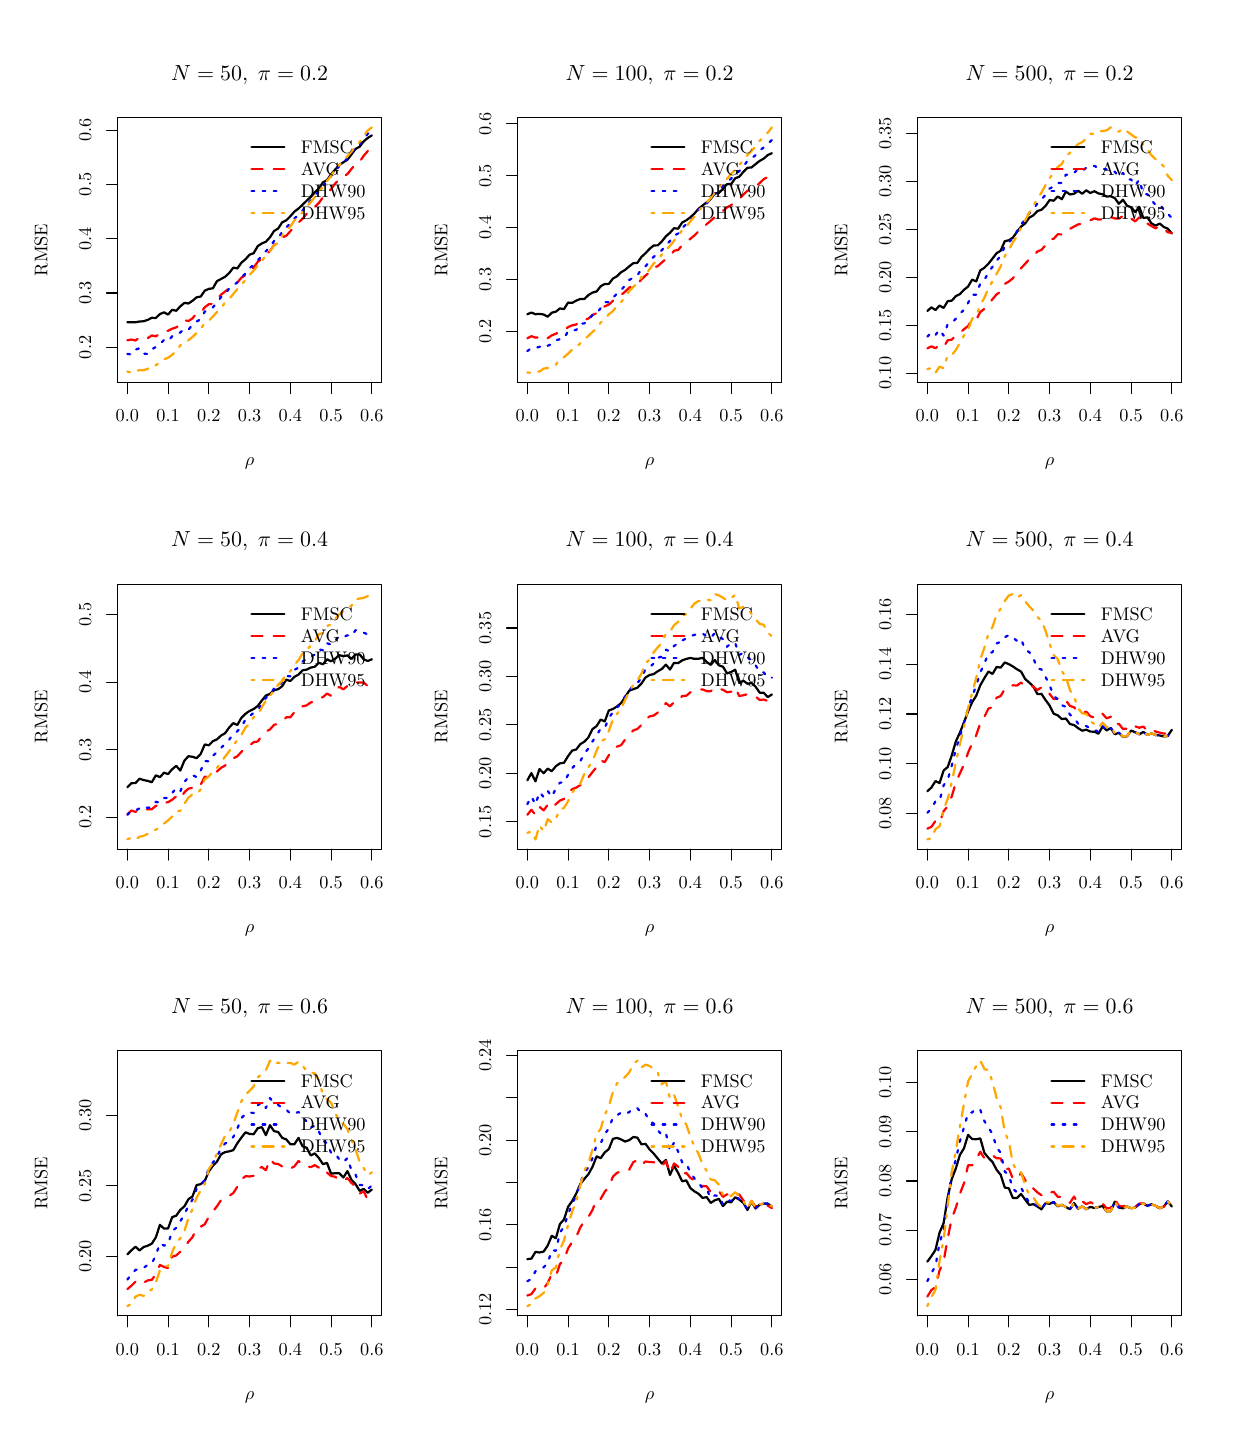
\begin{tikzpicture}[x=1pt,y=1pt]
\definecolor[named]{fillColor}{rgb}{1.00,1.00,1.00}
\path[use as bounding box,fill=fillColor,fill opacity=0.00] (0,0) rectangle (433.62,505.89);
\begin{scope}
\path[clip] ( 32.47,377.65) rectangle (127.91,473.42);
\definecolor[named]{drawColor}{rgb}{0.00,0.00,0.00}

\path[draw=drawColor,line width= 0.8pt,line join=round,line cap=round] ( 36.01,399.47) --
	( 37.48,399.47) --
	( 38.95,399.41) --
	( 40.42,399.71) --
	( 41.90,399.80) --
	( 43.37,400.28) --
	( 44.84,401.04) --
	( 46.32,400.99) --
	( 47.79,402.40) --
	( 49.26,403.03) --
	( 50.73,402.22) --
	( 52.21,403.94) --
	( 53.68,403.59) --
	( 55.15,405.19) --
	( 56.63,406.43) --
	( 58.10,406.22) --
	( 59.57,407.19) --
	( 61.04,408.46) --
	( 62.52,408.72) --
	( 63.99,410.85) --
	( 65.46,411.50) --
	( 66.93,411.71) --
	( 68.41,414.31) --
	( 69.88,415.08) --
	( 71.35,415.88) --
	( 72.83,417.24) --
	( 74.30,419.17) --
	( 75.77,418.89) --
	( 77.24,420.97) --
	( 78.72,422.22) --
	( 80.19,423.86) --
	( 81.66,424.39) --
	( 83.14,426.96) --
	( 84.61,427.92) --
	( 86.08,428.52) --
	( 87.55,430.12) --
	( 89.03,432.42) --
	( 90.50,433.29) --
	( 91.97,435.56) --
	( 93.44,436.26) --
	( 94.92,437.75) --
	( 96.39,439.42) --
	( 97.86,440.52) --
	( 99.34,441.93) --
	(100.81,443.36) --
	(102.28,444.71) --
	(103.75,446.39) --
	(105.23,447.80) --
	(106.70,450.00) --
	(108.17,450.78) --
	(109.65,452.94) --
	(111.12,454.63) --
	(112.59,456.24) --
	(114.06,457.24) --
	(115.54,458.16) --
	(117.01,460.09) --
	(118.48,462.06) --
	(119.95,462.87) --
	(121.43,464.80) --
	(122.90,466.05) --
	(124.37,466.95);
\end{scope}
\begin{scope}
\path[clip] (  0.00,  0.00) rectangle (433.62,505.89);
\definecolor[named]{drawColor}{rgb}{0.00,0.00,0.00}

\path[draw=drawColor,line width= 0.4pt,line join=round,line cap=round] ( 36.01,377.65) -- (124.37,377.65);

\path[draw=drawColor,line width= 0.4pt,line join=round,line cap=round] ( 36.01,377.65) -- ( 36.01,373.69);

\path[draw=drawColor,line width= 0.4pt,line join=round,line cap=round] ( 50.73,377.65) -- ( 50.73,373.69);

\path[draw=drawColor,line width= 0.4pt,line join=round,line cap=round] ( 65.46,377.65) -- ( 65.46,373.69);

\path[draw=drawColor,line width= 0.4pt,line join=round,line cap=round] ( 80.19,377.65) -- ( 80.19,373.69);

\path[draw=drawColor,line width= 0.4pt,line join=round,line cap=round] ( 94.92,377.65) -- ( 94.92,373.69);

\path[draw=drawColor,line width= 0.4pt,line join=round,line cap=round] (109.65,377.65) -- (109.65,373.69);

\path[draw=drawColor,line width= 0.4pt,line join=round,line cap=round] (124.37,377.65) -- (124.37,373.69);

\node[text=drawColor,anchor=base,inner sep=0pt, outer sep=0pt, scale=  0.66] at ( 36.01,363.40) {0.0};

\node[text=drawColor,anchor=base,inner sep=0pt, outer sep=0pt, scale=  0.66] at ( 50.73,363.40) {0.1};

\node[text=drawColor,anchor=base,inner sep=0pt, outer sep=0pt, scale=  0.66] at ( 65.46,363.40) {0.2};

\node[text=drawColor,anchor=base,inner sep=0pt, outer sep=0pt, scale=  0.66] at ( 80.19,363.40) {0.3};

\node[text=drawColor,anchor=base,inner sep=0pt, outer sep=0pt, scale=  0.66] at ( 94.92,363.40) {0.4};

\node[text=drawColor,anchor=base,inner sep=0pt, outer sep=0pt, scale=  0.66] at (109.65,363.40) {0.5};

\node[text=drawColor,anchor=base,inner sep=0pt, outer sep=0pt, scale=  0.66] at (124.37,363.40) {0.6};

\path[draw=drawColor,line width= 0.4pt,line join=round,line cap=round] ( 32.47,390.37) -- ( 32.47,468.88);

\path[draw=drawColor,line width= 0.4pt,line join=round,line cap=round] ( 32.47,390.37) -- ( 28.51,390.37);

\path[draw=drawColor,line width= 0.4pt,line join=round,line cap=round] ( 32.47,410.00) -- ( 28.51,410.00);

\path[draw=drawColor,line width= 0.4pt,line join=round,line cap=round] ( 32.47,429.62) -- ( 28.51,429.62);

\path[draw=drawColor,line width= 0.4pt,line join=round,line cap=round] ( 32.47,449.25) -- ( 28.51,449.25);

\path[draw=drawColor,line width= 0.4pt,line join=round,line cap=round] ( 32.47,468.88) -- ( 28.51,468.88);

\node[text=drawColor,rotate= 90.00,anchor=base,inner sep=0pt, outer sep=0pt, scale=  0.66] at ( 22.97,390.37) {0.2};

\node[text=drawColor,rotate= 90.00,anchor=base,inner sep=0pt, outer sep=0pt, scale=  0.66] at ( 22.97,410.00) {0.3};

\node[text=drawColor,rotate= 90.00,anchor=base,inner sep=0pt, outer sep=0pt, scale=  0.66] at ( 22.97,429.62) {0.4};

\node[text=drawColor,rotate= 90.00,anchor=base,inner sep=0pt, outer sep=0pt, scale=  0.66] at ( 22.97,449.25) {0.5};

\node[text=drawColor,rotate= 90.00,anchor=base,inner sep=0pt, outer sep=0pt, scale=  0.66] at ( 22.97,468.88) {0.6};

\path[draw=drawColor,line width= 0.4pt,line join=round,line cap=round] ( 32.47,377.65) --
	(127.91,377.65) --
	(127.91,473.42) --
	( 32.47,473.42) --
	( 32.47,377.65);
\end{scope}
\begin{scope}
\path[clip] (  0.00,337.26) rectangle (144.54,505.89);
\definecolor[named]{drawColor}{rgb}{0.00,0.00,0.00}

\node[text=drawColor,anchor=base,inner sep=0pt, outer sep=0pt, scale=  0.79] at ( 80.19,486.92) {\bfseries $N=50, \;\pi=0.2$};

\node[text=drawColor,anchor=base,inner sep=0pt, outer sep=0pt, scale=  0.66] at ( 80.19,347.56) {$\rho$};

\node[text=drawColor,rotate= 90.00,anchor=base,inner sep=0pt, outer sep=0pt, scale=  0.66] at (  7.13,425.53) {RMSE};
\end{scope}
\begin{scope}
\path[clip] ( 32.47,377.65) rectangle (127.91,473.42);
\definecolor[named]{drawColor}{rgb}{1.00,0.00,0.00}

\path[draw=drawColor,line width= 0.8pt,dash pattern=on 4pt off 4pt ,line join=round,line cap=round] ( 36.01,392.90) --
	( 37.48,393.20) --
	( 38.95,392.84) --
	( 40.42,393.97) --
	( 41.90,393.41) --
	( 43.37,393.70) --
	( 44.84,394.67) --
	( 46.32,394.33) --
	( 47.79,395.39) --
	( 49.26,396.30) --
	( 50.73,396.37) --
	( 52.21,397.11) --
	( 53.68,397.59) --
	( 55.15,398.61) --
	( 56.63,400.23) --
	( 58.10,399.85) --
	( 59.57,400.86) --
	( 61.04,402.76) --
	( 62.52,402.81) --
	( 63.99,404.86) --
	( 65.46,405.95) --
	( 66.93,406.12) --
	( 68.41,407.69) --
	( 69.88,409.39) --
	( 71.35,410.58) --
	( 72.83,411.67) --
	( 74.30,413.10) --
	( 75.77,413.80) --
	( 77.24,415.57) --
	( 78.72,416.45) --
	( 80.19,418.36) --
	( 81.66,419.20) --
	( 83.14,421.26) --
	( 84.61,422.48) --
	( 86.08,423.78) --
	( 87.55,425.22) --
	( 89.03,427.30) --
	( 90.50,428.21) --
	( 91.97,430.05) --
	( 93.44,430.69) --
	( 94.92,432.33) --
	( 96.39,434.26) --
	( 97.86,435.48) --
	( 99.34,436.84) --
	(100.81,438.65) --
	(102.28,439.82) --
	(103.75,441.08) --
	(105.23,442.56) --
	(106.70,444.59) --
	(108.17,446.14) --
	(109.65,447.51) --
	(111.12,449.60) --
	(112.59,451.04) --
	(114.06,451.97) --
	(115.54,453.00) --
	(117.01,454.84) --
	(118.48,456.64) --
	(119.95,457.37) --
	(121.43,459.60) --
	(122.90,461.30) --
	(124.37,461.90);
\definecolor[named]{drawColor}{rgb}{0.00,0.00,1.00}

\path[draw=drawColor,line width= 0.8pt,dash pattern=on 1pt off 3pt ,line join=round,line cap=round] ( 36.01,387.99) --
	( 37.48,387.83) --
	( 38.95,389.53) --
	( 40.42,390.06) --
	( 41.90,388.10) --
	( 43.37,387.97) --
	( 44.84,389.67) --
	( 46.32,390.50) --
	( 47.79,391.44) --
	( 49.26,393.07) --
	( 50.73,392.60) --
	( 52.21,394.37) --
	( 53.68,394.66) --
	( 55.15,395.77) --
	( 56.63,397.08) --
	( 58.10,396.80) --
	( 59.57,398.50) --
	( 61.04,399.68) --
	( 62.52,400.55) --
	( 63.99,403.32) --
	( 65.46,403.75) --
	( 66.93,404.82) --
	( 68.41,406.61) --
	( 69.88,408.51) --
	( 71.35,409.62) --
	( 72.83,411.69) --
	( 74.30,412.73) --
	( 75.77,413.85) --
	( 77.24,415.69) --
	( 78.72,417.06) --
	( 80.19,419.06) --
	( 81.66,420.06) --
	( 83.14,421.84) --
	( 84.61,423.39) --
	( 86.08,425.10) --
	( 87.55,426.68) --
	( 89.03,428.77) --
	( 90.50,429.68) --
	( 91.97,432.18) --
	( 93.44,433.64) --
	( 94.92,435.22) --
	( 96.39,436.96) --
	( 97.86,438.24) --
	( 99.34,439.80) --
	(100.81,441.80) --
	(102.28,443.40) --
	(103.75,445.27) --
	(105.23,446.72) --
	(106.70,448.79) --
	(108.17,450.27) --
	(109.65,452.29) --
	(111.12,454.38) --
	(112.59,455.75) --
	(114.06,457.10) --
	(115.54,458.70) --
	(117.01,460.46) --
	(118.48,462.67) --
	(119.95,463.56) --
	(121.43,465.64) --
	(122.90,467.55) --
	(124.37,468.42);
\definecolor[named]{drawColor}{rgb}{1.00,0.65,0.00}

\path[draw=drawColor,line width= 0.8pt,dash pattern=on 1pt off 3pt on 4pt off 3pt ,line join=round,line cap=round] ( 36.01,381.65) --
	( 37.48,381.20) --
	( 38.95,381.69) --
	( 40.42,382.15) --
	( 41.90,382.10) --
	( 43.37,382.56) --
	( 44.84,383.91) --
	( 46.32,383.88) --
	( 47.79,385.04) --
	( 49.26,386.04) --
	( 50.73,386.59) --
	( 52.21,387.72) --
	( 53.68,388.96) --
	( 55.15,391.10) --
	( 56.63,391.91) --
	( 58.10,392.95) --
	( 59.57,394.15) --
	( 61.04,395.56) --
	( 62.52,396.92) --
	( 63.99,399.31) --
	( 65.46,400.10) --
	( 66.93,401.49) --
	( 68.41,403.10) --
	( 69.88,404.49) --
	( 71.35,406.68) --
	( 72.83,407.84) --
	( 74.30,409.64) --
	( 75.77,411.46) --
	( 77.24,413.02) --
	( 78.72,414.74) --
	( 80.19,416.56) --
	( 81.66,418.11) --
	( 83.14,419.97) --
	( 84.61,421.48) --
	( 86.08,423.67) --
	( 87.55,425.15) --
	( 89.03,427.16) --
	( 90.50,428.18) --
	( 91.97,430.75) --
	( 93.44,432.41) --
	( 94.92,434.03) --
	( 96.39,436.22) --
	( 97.86,437.60) --
	( 99.34,439.08) --
	(100.81,441.24) --
	(102.28,442.83) --
	(103.75,444.80) --
	(105.23,446.18) --
	(106.70,448.66) --
	(108.17,450.46) --
	(109.65,452.40) --
	(111.12,454.59) --
	(112.59,456.17) --
	(114.06,457.68) --
	(115.54,459.45) --
	(117.01,461.12) --
	(118.48,463.24) --
	(119.95,464.57) --
	(121.43,466.80) --
	(122.90,468.74) --
	(124.37,469.87);
\definecolor[named]{drawColor}{rgb}{0.00,0.00,0.00}

\path[draw=drawColor,line width= 0.8pt,line join=round,line cap=round] ( 80.89,462.63) -- ( 92.77,462.63);
\definecolor[named]{drawColor}{rgb}{1.00,0.00,0.00}

\path[draw=drawColor,line width= 0.8pt,dash pattern=on 4pt off 4pt ,line join=round,line cap=round] ( 80.89,454.71) -- ( 92.77,454.71);
\definecolor[named]{drawColor}{rgb}{0.00,0.00,1.00}

\path[draw=drawColor,line width= 0.8pt,dash pattern=on 1pt off 3pt ,line join=round,line cap=round] ( 80.89,446.79) -- ( 92.77,446.79);
\definecolor[named]{drawColor}{rgb}{1.00,0.65,0.00}

\path[draw=drawColor,line width= 0.8pt,dash pattern=on 1pt off 3pt on 4pt off 3pt ,line join=round,line cap=round] ( 80.89,438.87) -- ( 92.77,438.87);
\definecolor[named]{drawColor}{rgb}{0.00,0.00,0.00}

\node[text=drawColor,anchor=base west,inner sep=0pt, outer sep=0pt, scale=  0.66] at ( 98.71,460.35) {FMSC};

\node[text=drawColor,anchor=base west,inner sep=0pt, outer sep=0pt, scale=  0.66] at ( 98.71,452.43) {AVG};

\node[text=drawColor,anchor=base west,inner sep=0pt, outer sep=0pt, scale=  0.66] at ( 98.71,444.51) {DHW90};

\node[text=drawColor,anchor=base west,inner sep=0pt, outer sep=0pt, scale=  0.66] at ( 98.71,436.59) {DHW95};
\end{scope}
\begin{scope}
\path[clip] (177.01,377.65) rectangle (272.45,473.42);
\definecolor[named]{drawColor}{rgb}{0.00,0.00,0.00}

\path[draw=drawColor,line width= 0.8pt,line join=round,line cap=round] (180.55,402.31) --
	(182.02,402.94) --
	(183.49,402.35) --
	(184.96,402.47) --
	(186.44,402.24) --
	(187.91,401.44) --
	(189.38,402.89) --
	(190.86,403.28) --
	(192.33,404.44) --
	(193.80,404.18) --
	(195.27,406.55) --
	(196.75,406.44) --
	(198.22,407.25) --
	(199.69,407.86) --
	(201.17,407.85) --
	(202.64,409.28) --
	(204.11,410.16) --
	(205.58,410.57) --
	(207.06,412.45) --
	(208.53,413.28) --
	(210.00,413.30) --
	(211.47,415.21) --
	(212.95,416.07) --
	(214.42,417.51) --
	(215.89,418.36) --
	(217.37,419.64) --
	(218.84,420.78) --
	(220.31,420.91) --
	(221.78,423.04) --
	(223.26,424.40) --
	(224.73,425.97) --
	(226.20,427.19) --
	(227.68,427.23) --
	(229.15,428.64) --
	(230.62,430.50) --
	(232.09,431.77) --
	(233.57,433.43) --
	(235.04,433.24) --
	(236.51,435.50) --
	(237.98,436.26) --
	(239.46,437.37) --
	(240.93,438.72) --
	(242.40,440.44) --
	(243.88,441.62) --
	(245.35,442.77) --
	(246.82,443.98) --
	(248.29,445.98) --
	(249.77,446.13) --
	(251.24,447.68) --
	(252.71,449.35) --
	(254.19,449.38) --
	(255.66,451.45) --
	(257.13,452.04) --
	(258.60,453.74) --
	(260.08,455.26) --
	(261.55,455.37) --
	(263.02,456.57) --
	(264.50,457.74) --
	(265.97,458.58) --
	(267.44,459.86) --
	(268.91,460.52);
\end{scope}
\begin{scope}
\path[clip] (  0.00,  0.00) rectangle (433.62,505.89);
\definecolor[named]{drawColor}{rgb}{0.00,0.00,0.00}

\path[draw=drawColor,line width= 0.4pt,line join=round,line cap=round] (180.55,377.65) -- (268.91,377.65);

\path[draw=drawColor,line width= 0.4pt,line join=round,line cap=round] (180.55,377.65) -- (180.55,373.69);

\path[draw=drawColor,line width= 0.4pt,line join=round,line cap=round] (195.27,377.65) -- (195.27,373.69);

\path[draw=drawColor,line width= 0.4pt,line join=round,line cap=round] (210.00,377.65) -- (210.00,373.69);

\path[draw=drawColor,line width= 0.4pt,line join=round,line cap=round] (224.73,377.65) -- (224.73,373.69);

\path[draw=drawColor,line width= 0.4pt,line join=round,line cap=round] (239.46,377.65) -- (239.46,373.69);

\path[draw=drawColor,line width= 0.4pt,line join=round,line cap=round] (254.19,377.65) -- (254.19,373.69);

\path[draw=drawColor,line width= 0.4pt,line join=round,line cap=round] (268.91,377.65) -- (268.91,373.69);

\node[text=drawColor,anchor=base,inner sep=0pt, outer sep=0pt, scale=  0.66] at (180.55,363.40) {0.0};

\node[text=drawColor,anchor=base,inner sep=0pt, outer sep=0pt, scale=  0.66] at (195.27,363.40) {0.1};

\node[text=drawColor,anchor=base,inner sep=0pt, outer sep=0pt, scale=  0.66] at (210.00,363.40) {0.2};

\node[text=drawColor,anchor=base,inner sep=0pt, outer sep=0pt, scale=  0.66] at (224.73,363.40) {0.3};

\node[text=drawColor,anchor=base,inner sep=0pt, outer sep=0pt, scale=  0.66] at (239.46,363.40) {0.4};

\node[text=drawColor,anchor=base,inner sep=0pt, outer sep=0pt, scale=  0.66] at (254.19,363.40) {0.5};

\node[text=drawColor,anchor=base,inner sep=0pt, outer sep=0pt, scale=  0.66] at (268.91,363.40) {0.6};

\path[draw=drawColor,line width= 0.4pt,line join=round,line cap=round] (177.01,396.12) -- (177.01,471.23);

\path[draw=drawColor,line width= 0.4pt,line join=round,line cap=round] (177.01,396.12) -- (173.05,396.12);

\path[draw=drawColor,line width= 0.4pt,line join=round,line cap=round] (177.01,414.90) -- (173.05,414.90);

\path[draw=drawColor,line width= 0.4pt,line join=round,line cap=round] (177.01,433.68) -- (173.05,433.68);

\path[draw=drawColor,line width= 0.4pt,line join=round,line cap=round] (177.01,452.45) -- (173.05,452.45);

\path[draw=drawColor,line width= 0.4pt,line join=round,line cap=round] (177.01,471.23) -- (173.05,471.23);

\node[text=drawColor,rotate= 90.00,anchor=base,inner sep=0pt, outer sep=0pt, scale=  0.66] at (167.51,396.12) {0.2};

\node[text=drawColor,rotate= 90.00,anchor=base,inner sep=0pt, outer sep=0pt, scale=  0.66] at (167.51,414.90) {0.3};

\node[text=drawColor,rotate= 90.00,anchor=base,inner sep=0pt, outer sep=0pt, scale=  0.66] at (167.51,433.68) {0.4};

\node[text=drawColor,rotate= 90.00,anchor=base,inner sep=0pt, outer sep=0pt, scale=  0.66] at (167.51,452.45) {0.5};

\node[text=drawColor,rotate= 90.00,anchor=base,inner sep=0pt, outer sep=0pt, scale=  0.66] at (167.51,471.23) {0.6};

\path[draw=drawColor,line width= 0.4pt,line join=round,line cap=round] (177.01,377.65) --
	(272.45,377.65) --
	(272.45,473.42) --
	(177.01,473.42) --
	(177.01,377.65);
\end{scope}
\begin{scope}
\path[clip] (144.54,337.26) rectangle (289.08,505.89);
\definecolor[named]{drawColor}{rgb}{0.00,0.00,0.00}

\node[text=drawColor,anchor=base,inner sep=0pt, outer sep=0pt, scale=  0.79] at (224.73,486.92) {\bfseries $N=100, \;\pi=0.2$};

\node[text=drawColor,anchor=base,inner sep=0pt, outer sep=0pt, scale=  0.66] at (224.73,347.56) {$\rho$};

\node[text=drawColor,rotate= 90.00,anchor=base,inner sep=0pt, outer sep=0pt, scale=  0.66] at (151.67,425.53) {RMSE};
\end{scope}
\begin{scope}
\path[clip] (177.01,377.65) rectangle (272.45,473.42);
\definecolor[named]{drawColor}{rgb}{1.00,0.00,0.00}

\path[draw=drawColor,line width= 0.8pt,dash pattern=on 4pt off 4pt ,line join=round,line cap=round] (180.55,393.63) --
	(182.02,394.41) --
	(183.49,393.87) --
	(184.96,394.07) --
	(186.44,394.69) --
	(187.91,393.69) --
	(189.38,394.70) --
	(190.86,395.28) --
	(192.33,396.19) --
	(193.80,396.54) --
	(195.27,397.69) --
	(196.75,398.31) --
	(198.22,398.63) --
	(199.69,400.00) --
	(201.17,400.20) --
	(202.64,400.81) --
	(204.11,402.04) --
	(205.58,402.75) --
	(207.06,404.44) --
	(208.53,405.18) --
	(210.00,405.84) --
	(211.47,407.16) --
	(212.95,408.50) --
	(214.42,409.23) --
	(215.89,410.50) --
	(217.37,411.95) --
	(218.84,412.87) --
	(220.31,413.22) --
	(221.78,414.92) --
	(223.26,416.32) --
	(224.73,417.47) --
	(226.20,419.24) --
	(227.68,419.70) --
	(229.15,421.03) --
	(230.62,422.30) --
	(232.09,423.30) --
	(233.57,425.28) --
	(235.04,425.53) --
	(236.51,427.38) --
	(237.98,428.53) --
	(239.46,429.59) --
	(240.93,430.82) --
	(242.40,432.27) --
	(243.88,433.32) --
	(245.35,434.89) --
	(246.82,436.12) --
	(248.29,437.45) --
	(249.77,438.59) --
	(251.24,439.65) --
	(252.71,440.93) --
	(254.19,441.75) --
	(255.66,443.04) --
	(257.13,444.01) --
	(258.60,445.54) --
	(260.08,446.97) --
	(261.55,447.28) --
	(263.02,448.38) --
	(264.50,449.74) --
	(265.97,451.14) --
	(267.44,451.94) --
	(268.91,453.28);
\definecolor[named]{drawColor}{rgb}{0.00,0.00,1.00}

\path[draw=drawColor,line width= 0.8pt,dash pattern=on 1pt off 3pt ,line join=round,line cap=round] (180.55,389.02) --
	(182.02,390.11) --
	(183.49,390.20) --
	(184.96,390.54) --
	(186.44,391.36) --
	(187.91,390.96) --
	(189.38,391.58) --
	(190.86,392.92) --
	(192.33,393.32) --
	(193.80,393.59) --
	(195.27,396.19) --
	(196.75,396.47) --
	(198.22,396.65) --
	(199.69,398.85) --
	(201.17,399.04) --
	(202.64,400.10) --
	(204.11,402.13) --
	(205.58,402.58) --
	(207.06,404.56) --
	(208.53,406.72) --
	(210.00,406.69) --
	(211.47,408.25) --
	(212.95,409.80) --
	(214.42,410.96) --
	(215.89,412.83) --
	(217.37,414.70) --
	(218.84,415.58) --
	(220.31,416.33) --
	(221.78,418.73) --
	(223.26,419.68) --
	(224.73,421.37) --
	(226.20,423.09) --
	(227.68,424.07) --
	(229.15,425.47) --
	(230.62,427.28) --
	(232.09,428.78) --
	(233.57,430.79) --
	(235.04,431.50) --
	(236.51,433.54) --
	(237.98,434.84) --
	(239.46,436.17) --
	(240.93,437.95) --
	(242.40,440.14) --
	(243.88,441.26) --
	(245.35,442.37) --
	(246.82,444.09) --
	(248.29,445.89) --
	(249.77,447.31) --
	(251.24,448.68) --
	(252.71,450.07) --
	(254.19,451.33) --
	(255.66,452.91) --
	(257.13,454.05) --
	(258.60,455.67) --
	(260.08,457.75) --
	(261.55,458.56) --
	(263.02,459.84) --
	(264.50,461.53) --
	(265.97,462.59) --
	(267.44,463.93) --
	(268.91,465.31);
\definecolor[named]{drawColor}{rgb}{1.00,0.65,0.00}

\path[draw=drawColor,line width= 0.8pt,dash pattern=on 1pt off 3pt on 4pt off 3pt ,line join=round,line cap=round] (180.55,381.26) --
	(182.02,381.20) --
	(183.49,381.72) --
	(184.96,381.59) --
	(186.44,382.70) --
	(187.91,382.87) --
	(189.38,383.27) --
	(190.86,384.13) --
	(192.33,386.13) --
	(193.80,386.83) --
	(195.27,388.07) --
	(196.75,389.59) --
	(198.22,390.27) --
	(199.69,391.88) --
	(201.17,393.21) --
	(202.64,394.54) --
	(204.11,395.96) --
	(205.58,397.23) --
	(207.06,399.31) --
	(208.53,400.59) --
	(210.00,402.31) --
	(211.47,403.46) --
	(212.95,405.32) --
	(214.42,406.68) --
	(215.89,408.60) --
	(217.37,410.69) --
	(218.84,412.22) --
	(220.31,413.48) --
	(221.78,415.70) --
	(223.26,416.54) --
	(224.73,418.61) --
	(226.20,420.63) --
	(227.68,422.01) --
	(229.15,423.87) --
	(230.62,425.48) --
	(232.09,427.04) --
	(233.57,428.86) --
	(235.04,430.73) --
	(236.51,432.72) --
	(237.98,433.92) --
	(239.46,435.87) --
	(240.93,437.61) --
	(242.40,439.65) --
	(243.88,441.18) --
	(245.35,442.70) --
	(246.82,444.33) --
	(248.29,446.37) --
	(249.77,448.22) --
	(251.24,449.65) --
	(252.71,451.22) --
	(254.19,453.10) --
	(255.66,454.57) --
	(257.13,456.19) --
	(258.60,458.05) --
	(260.08,459.82) --
	(261.55,461.36) --
	(263.02,462.93) --
	(264.50,465.01) --
	(265.97,466.30) --
	(267.44,467.97) --
	(268.91,469.87);
\definecolor[named]{drawColor}{rgb}{0.00,0.00,0.00}

\path[draw=drawColor,line width= 0.8pt,line join=round,line cap=round] (225.43,462.63) -- (237.31,462.63);
\definecolor[named]{drawColor}{rgb}{1.00,0.00,0.00}

\path[draw=drawColor,line width= 0.8pt,dash pattern=on 4pt off 4pt ,line join=round,line cap=round] (225.43,454.71) -- (237.31,454.71);
\definecolor[named]{drawColor}{rgb}{0.00,0.00,1.00}

\path[draw=drawColor,line width= 0.8pt,dash pattern=on 1pt off 3pt ,line join=round,line cap=round] (225.43,446.79) -- (237.31,446.79);
\definecolor[named]{drawColor}{rgb}{1.00,0.65,0.00}

\path[draw=drawColor,line width= 0.8pt,dash pattern=on 1pt off 3pt on 4pt off 3pt ,line join=round,line cap=round] (225.43,438.87) -- (237.31,438.87);
\definecolor[named]{drawColor}{rgb}{0.00,0.00,0.00}

\node[text=drawColor,anchor=base west,inner sep=0pt, outer sep=0pt, scale=  0.66] at (243.25,460.35) {FMSC};

\node[text=drawColor,anchor=base west,inner sep=0pt, outer sep=0pt, scale=  0.66] at (243.25,452.43) {AVG};

\node[text=drawColor,anchor=base west,inner sep=0pt, outer sep=0pt, scale=  0.66] at (243.25,444.51) {DHW90};

\node[text=drawColor,anchor=base west,inner sep=0pt, outer sep=0pt, scale=  0.66] at (243.25,436.59) {DHW95};
\end{scope}
\begin{scope}
\path[clip] (321.55,377.65) rectangle (416.99,473.42);
\definecolor[named]{drawColor}{rgb}{0.00,0.00,0.00}

\path[draw=drawColor,line width= 0.8pt,line join=round,line cap=round] (325.09,403.51) --
	(326.56,404.81) --
	(328.03,403.86) --
	(329.50,405.48) --
	(330.98,404.61) --
	(332.45,407.06) --
	(333.92,407.25) --
	(335.40,408.88) --
	(336.87,409.63) --
	(338.34,411.18) --
	(339.81,412.34) --
	(341.29,414.85) --
	(342.76,414.20) --
	(344.23,418.20) --
	(345.71,419.12) --
	(347.18,420.62) --
	(348.65,422.48) --
	(350.12,424.39) --
	(351.60,425.29) --
	(353.07,428.74) --
	(354.54,429.06) --
	(356.01,430.03) --
	(357.49,432.10) --
	(358.96,433.99) --
	(360.43,435.15) --
	(361.91,437.24) --
	(363.38,438.05) --
	(364.85,439.62) --
	(366.32,440.09) --
	(367.80,441.47) --
	(369.27,443.60) --
	(370.74,443.36) --
	(372.22,444.89) --
	(373.69,443.89) --
	(375.16,446.65) --
	(376.63,445.61) --
	(378.11,445.87) --
	(379.58,446.95) --
	(381.05,445.87) --
	(382.52,447.12) --
	(384.00,446.14) --
	(385.47,446.79) --
	(386.94,445.97) --
	(388.42,445.69) --
	(389.89,444.85) --
	(391.36,444.99) --
	(392.83,444.29) --
	(394.31,442.25) --
	(395.78,443.71) --
	(397.25,441.55) --
	(398.73,441.01) --
	(400.20,439.23) --
	(401.67,441.12) --
	(403.14,437.11) --
	(404.62,437.36) --
	(406.09,435.16) --
	(407.56,434.34) --
	(409.04,435.11) --
	(410.51,433.89) --
	(411.98,433.24) --
	(413.45,431.52);
\end{scope}
\begin{scope}
\path[clip] (  0.00,  0.00) rectangle (433.62,505.89);
\definecolor[named]{drawColor}{rgb}{0.00,0.00,0.00}

\path[draw=drawColor,line width= 0.4pt,line join=round,line cap=round] (325.09,377.65) -- (413.45,377.65);

\path[draw=drawColor,line width= 0.4pt,line join=round,line cap=round] (325.09,377.65) -- (325.09,373.69);

\path[draw=drawColor,line width= 0.4pt,line join=round,line cap=round] (339.81,377.65) -- (339.81,373.69);

\path[draw=drawColor,line width= 0.4pt,line join=round,line cap=round] (354.54,377.65) -- (354.54,373.69);

\path[draw=drawColor,line width= 0.4pt,line join=round,line cap=round] (369.27,377.65) -- (369.27,373.69);

\path[draw=drawColor,line width= 0.4pt,line join=round,line cap=round] (384.00,377.65) -- (384.00,373.69);

\path[draw=drawColor,line width= 0.4pt,line join=round,line cap=round] (398.73,377.65) -- (398.73,373.69);

\path[draw=drawColor,line width= 0.4pt,line join=round,line cap=round] (413.45,377.65) -- (413.45,373.69);

\node[text=drawColor,anchor=base,inner sep=0pt, outer sep=0pt, scale=  0.66] at (325.09,363.40) {0.0};

\node[text=drawColor,anchor=base,inner sep=0pt, outer sep=0pt, scale=  0.66] at (339.81,363.40) {0.1};

\node[text=drawColor,anchor=base,inner sep=0pt, outer sep=0pt, scale=  0.66] at (354.54,363.40) {0.2};

\node[text=drawColor,anchor=base,inner sep=0pt, outer sep=0pt, scale=  0.66] at (369.27,363.40) {0.3};

\node[text=drawColor,anchor=base,inner sep=0pt, outer sep=0pt, scale=  0.66] at (384.00,363.40) {0.4};

\node[text=drawColor,anchor=base,inner sep=0pt, outer sep=0pt, scale=  0.66] at (398.73,363.40) {0.5};

\node[text=drawColor,anchor=base,inner sep=0pt, outer sep=0pt, scale=  0.66] at (413.45,363.40) {0.6};

\path[draw=drawColor,line width= 0.4pt,line join=round,line cap=round] (321.55,381.08) -- (321.55,467.59);

\path[draw=drawColor,line width= 0.4pt,line join=round,line cap=round] (321.55,381.08) -- (317.59,381.08);

\path[draw=drawColor,line width= 0.4pt,line join=round,line cap=round] (321.55,398.38) -- (317.59,398.38);

\path[draw=drawColor,line width= 0.4pt,line join=round,line cap=round] (321.55,415.68) -- (317.59,415.68);

\path[draw=drawColor,line width= 0.4pt,line join=round,line cap=round] (321.55,432.99) -- (317.59,432.99);

\path[draw=drawColor,line width= 0.4pt,line join=round,line cap=round] (321.55,450.29) -- (317.59,450.29);

\path[draw=drawColor,line width= 0.4pt,line join=round,line cap=round] (321.55,467.59) -- (317.59,467.59);

\node[text=drawColor,rotate= 90.00,anchor=base,inner sep=0pt, outer sep=0pt, scale=  0.66] at (312.05,381.08) {0.10};

\node[text=drawColor,rotate= 90.00,anchor=base,inner sep=0pt, outer sep=0pt, scale=  0.66] at (312.05,398.38) {0.15};

\node[text=drawColor,rotate= 90.00,anchor=base,inner sep=0pt, outer sep=0pt, scale=  0.66] at (312.05,415.68) {0.20};

\node[text=drawColor,rotate= 90.00,anchor=base,inner sep=0pt, outer sep=0pt, scale=  0.66] at (312.05,432.99) {0.25};

\node[text=drawColor,rotate= 90.00,anchor=base,inner sep=0pt, outer sep=0pt, scale=  0.66] at (312.05,450.29) {0.30};

\node[text=drawColor,rotate= 90.00,anchor=base,inner sep=0pt, outer sep=0pt, scale=  0.66] at (312.05,467.59) {0.35};

\path[draw=drawColor,line width= 0.4pt,line join=round,line cap=round] (321.55,377.65) --
	(416.99,377.65) --
	(416.99,473.42) --
	(321.55,473.42) --
	(321.55,377.65);
\end{scope}
\begin{scope}
\path[clip] (289.08,337.26) rectangle (433.62,505.89);
\definecolor[named]{drawColor}{rgb}{0.00,0.00,0.00}

\node[text=drawColor,anchor=base,inner sep=0pt, outer sep=0pt, scale=  0.79] at (369.27,486.92) {\bfseries $N=500, \;\pi=0.2$};

\node[text=drawColor,anchor=base,inner sep=0pt, outer sep=0pt, scale=  0.66] at (369.27,347.56) {$\rho$};

\node[text=drawColor,rotate= 90.00,anchor=base,inner sep=0pt, outer sep=0pt, scale=  0.66] at (296.21,425.53) {RMSE};
\end{scope}
\begin{scope}
\path[clip] (321.55,377.65) rectangle (416.99,473.42);
\definecolor[named]{drawColor}{rgb}{1.00,0.00,0.00}

\path[draw=drawColor,line width= 0.8pt,dash pattern=on 4pt off 4pt ,line join=round,line cap=round] (325.09,389.97) --
	(326.56,390.74) --
	(328.03,390.05) --
	(329.50,391.19) --
	(330.98,390.54) --
	(332.45,392.90) --
	(333.92,393.16) --
	(335.40,394.67) --
	(336.87,395.59) --
	(338.34,396.91) --
	(339.81,398.10) --
	(341.29,400.49) --
	(342.76,400.32) --
	(344.23,403.16) --
	(345.71,404.27) --
	(347.18,406.03) --
	(348.65,407.78) --
	(350.12,409.54) --
	(351.60,410.47) --
	(353.07,413.29) --
	(354.54,414.16) --
	(356.01,415.32) --
	(357.49,417.41) --
	(358.96,418.98) --
	(360.43,420.55) --
	(361.91,422.26) --
	(363.38,423.32) --
	(364.85,424.99) --
	(366.32,425.60) --
	(367.80,427.28) --
	(369.27,429.40) --
	(370.74,429.60) --
	(372.22,431.21) --
	(373.69,431.18) --
	(375.16,432.74) --
	(376.63,433.19) --
	(378.11,434.01) --
	(379.58,434.80) --
	(381.05,435.03) --
	(382.52,435.71) --
	(384.00,436.27) --
	(385.47,436.97) --
	(386.94,436.54) --
	(388.42,436.56) --
	(389.89,436.78) --
	(391.36,437.47) --
	(392.83,436.94) --
	(394.31,436.91) --
	(395.78,437.84) --
	(397.25,436.61) --
	(398.73,436.89) --
	(400.20,435.90) --
	(401.67,437.30) --
	(403.14,434.88) --
	(404.62,435.11) --
	(406.09,434.20) --
	(407.56,433.39) --
	(409.04,434.20) --
	(410.51,433.29) --
	(411.98,431.97) --
	(413.45,431.68);
\definecolor[named]{drawColor}{rgb}{0.00,0.00,1.00}

\path[draw=drawColor,line width= 0.8pt,dash pattern=on 1pt off 3pt ,line join=round,line cap=round] (325.09,394.22) --
	(326.56,395.79) --
	(328.03,394.84) --
	(329.50,396.74) --
	(330.98,394.62) --
	(332.45,398.76) --
	(333.92,399.16) --
	(335.40,400.75) --
	(336.87,402.58) --
	(338.34,403.92) --
	(339.81,406.42) --
	(341.29,409.41) --
	(342.76,409.39) --
	(344.23,413.48) --
	(345.71,414.75) --
	(347.18,417.39) --
	(348.65,419.51) --
	(350.12,421.67) --
	(351.60,423.45) --
	(353.07,426.82) --
	(354.54,428.31) --
	(356.01,429.95) --
	(357.49,432.30) --
	(358.96,434.81) --
	(360.43,436.46) --
	(361.91,438.81) --
	(363.38,440.24) --
	(364.85,442.36) --
	(366.32,443.87) --
	(367.80,445.44) --
	(369.27,447.74) --
	(370.74,448.50) --
	(372.22,449.78) --
	(373.69,449.80) --
	(375.16,452.79) --
	(376.63,452.56) --
	(378.11,453.43) --
	(379.58,454.73) --
	(381.05,454.12) --
	(382.52,455.24) --
	(384.00,455.25) --
	(385.47,455.97) --
	(386.94,455.02) --
	(388.42,454.89) --
	(389.89,454.66) --
	(391.36,454.74) --
	(392.83,453.77) --
	(394.31,452.06) --
	(395.78,453.37) --
	(397.25,451.20) --
	(398.73,451.00) --
	(400.20,448.88) --
	(401.67,450.95) --
	(403.14,445.80) --
	(404.62,445.70) --
	(406.09,443.53) --
	(407.56,441.84) --
	(409.04,442.10) --
	(410.51,440.10) --
	(411.98,438.72) --
	(413.45,437.02);
\definecolor[named]{drawColor}{rgb}{1.00,0.65,0.00}

\path[draw=drawColor,line width= 0.8pt,dash pattern=on 1pt off 3pt on 4pt off 3pt ,line join=round,line cap=round] (325.09,382.47) --
	(326.56,382.95) --
	(328.03,381.20) --
	(329.50,383.42) --
	(330.98,382.79) --
	(332.45,387.50) --
	(333.92,387.66) --
	(335.40,389.41) --
	(336.87,392.06) --
	(338.34,394.69) --
	(339.81,396.84) --
	(341.29,400.68) --
	(342.76,401.78) --
	(344.23,405.67) --
	(345.71,408.28) --
	(347.18,411.79) --
	(348.65,414.27) --
	(350.12,416.93) --
	(351.60,419.62) --
	(353.07,423.30) --
	(354.54,425.55) --
	(356.01,428.39) --
	(357.49,430.49) --
	(358.96,433.62) --
	(360.43,436.19) --
	(361.91,439.08) --
	(363.38,441.65) --
	(364.85,443.90) --
	(366.32,446.28) --
	(367.80,448.99) --
	(369.27,451.53) --
	(370.74,453.40) --
	(372.22,455.59) --
	(373.69,456.62) --
	(375.16,459.41) --
	(376.63,460.66) --
	(378.11,462.19) --
	(379.58,463.84) --
	(381.05,464.51) --
	(382.52,465.83) --
	(384.00,467.52) --
	(385.47,467.62) --
	(386.94,468.43) --
	(388.42,468.50) --
	(389.89,468.80) --
	(391.36,469.87) --
	(392.83,468.98) --
	(394.31,468.29) --
	(395.78,469.43) --
	(397.25,468.41) --
	(398.73,467.29) --
	(400.20,466.22) --
	(401.67,466.20) --
	(403.14,463.61) --
	(404.62,461.86) --
	(406.09,459.76) --
	(407.56,458.37) --
	(409.04,457.42) --
	(410.51,455.71) --
	(411.98,452.35) --
	(413.45,450.81);
\definecolor[named]{drawColor}{rgb}{0.00,0.00,0.00}

\path[draw=drawColor,line width= 0.8pt,line join=round,line cap=round] (369.97,462.63) -- (381.85,462.63);
\definecolor[named]{drawColor}{rgb}{1.00,0.00,0.00}

\path[draw=drawColor,line width= 0.8pt,dash pattern=on 4pt off 4pt ,line join=round,line cap=round] (369.97,454.71) -- (381.85,454.71);
\definecolor[named]{drawColor}{rgb}{0.00,0.00,1.00}

\path[draw=drawColor,line width= 0.8pt,dash pattern=on 1pt off 3pt ,line join=round,line cap=round] (369.97,446.79) -- (381.85,446.79);
\definecolor[named]{drawColor}{rgb}{1.00,0.65,0.00}

\path[draw=drawColor,line width= 0.8pt,dash pattern=on 1pt off 3pt on 4pt off 3pt ,line join=round,line cap=round] (369.97,438.87) -- (381.85,438.87);
\definecolor[named]{drawColor}{rgb}{0.00,0.00,0.00}

\node[text=drawColor,anchor=base west,inner sep=0pt, outer sep=0pt, scale=  0.66] at (387.79,460.35) {FMSC};

\node[text=drawColor,anchor=base west,inner sep=0pt, outer sep=0pt, scale=  0.66] at (387.79,452.43) {AVG};

\node[text=drawColor,anchor=base west,inner sep=0pt, outer sep=0pt, scale=  0.66] at (387.79,444.51) {DHW90};

\node[text=drawColor,anchor=base west,inner sep=0pt, outer sep=0pt, scale=  0.66] at (387.79,436.59) {DHW95};
\end{scope}
\begin{scope}
\path[clip] ( 32.47,209.02) rectangle (127.91,304.79);
\definecolor[named]{drawColor}{rgb}{0.00,0.00,0.00}

\path[draw=drawColor,line width= 0.8pt,line join=round,line cap=round] ( 36.01,231.39) --
	( 37.48,232.89) --
	( 38.95,232.91) --
	( 40.42,234.50) --
	( 41.90,234.01) --
	( 43.37,233.72) --
	( 44.84,233.22) --
	( 46.32,235.72) --
	( 47.79,235.06) --
	( 49.26,236.66) --
	( 50.73,236.19) --
	( 52.21,237.93) --
	( 53.68,239.14) --
	( 55.15,237.45) --
	( 56.63,241.02) --
	( 58.10,242.64) --
	( 59.57,242.42) --
	( 61.04,241.92) --
	( 62.52,243.44) --
	( 63.99,246.87) --
	( 65.46,246.56) --
	( 66.93,248.07) --
	( 68.41,248.73) --
	( 69.88,250.09) --
	( 71.35,250.94) --
	( 72.83,253.02) --
	( 74.30,254.58) --
	( 75.77,253.92) --
	( 77.24,256.52) --
	( 78.72,257.97) --
	( 80.19,258.98) --
	( 81.66,259.68) --
	( 83.14,260.77) --
	( 84.61,262.74) --
	( 86.08,264.57) --
	( 87.55,265.13) --
	( 89.03,266.46) --
	( 90.50,266.85) --
	( 91.97,267.92) --
	( 93.44,270.30) --
	( 94.92,269.78) --
	( 96.39,271.31) --
	( 97.86,272.11) --
	( 99.34,273.67) --
	(100.81,273.92) --
	(102.28,274.65) --
	(103.75,274.96) --
	(105.23,276.39) --
	(106.70,275.83) --
	(108.17,277.62) --
	(109.65,276.93) --
	(111.12,277.88) --
	(112.59,279.14) --
	(114.06,278.79) --
	(115.54,279.04) --
	(117.01,277.80) --
	(118.48,279.41) --
	(119.95,279.41) --
	(121.43,277.63) --
	(122.90,277.05) --
	(124.37,277.66);
\end{scope}
\begin{scope}
\path[clip] (  0.00,  0.00) rectangle (433.62,505.89);
\definecolor[named]{drawColor}{rgb}{0.00,0.00,0.00}

\path[draw=drawColor,line width= 0.4pt,line join=round,line cap=round] ( 36.01,209.02) -- (124.37,209.02);

\path[draw=drawColor,line width= 0.4pt,line join=round,line cap=round] ( 36.01,209.02) -- ( 36.01,205.06);

\path[draw=drawColor,line width= 0.4pt,line join=round,line cap=round] ( 50.73,209.02) -- ( 50.73,205.06);

\path[draw=drawColor,line width= 0.4pt,line join=round,line cap=round] ( 65.46,209.02) -- ( 65.46,205.06);

\path[draw=drawColor,line width= 0.4pt,line join=round,line cap=round] ( 80.19,209.02) -- ( 80.19,205.06);

\path[draw=drawColor,line width= 0.4pt,line join=round,line cap=round] ( 94.92,209.02) -- ( 94.92,205.06);

\path[draw=drawColor,line width= 0.4pt,line join=round,line cap=round] (109.65,209.02) -- (109.65,205.06);

\path[draw=drawColor,line width= 0.4pt,line join=round,line cap=round] (124.37,209.02) -- (124.37,205.06);

\node[text=drawColor,anchor=base,inner sep=0pt, outer sep=0pt, scale=  0.66] at ( 36.01,194.77) {0.0};

\node[text=drawColor,anchor=base,inner sep=0pt, outer sep=0pt, scale=  0.66] at ( 50.73,194.77) {0.1};

\node[text=drawColor,anchor=base,inner sep=0pt, outer sep=0pt, scale=  0.66] at ( 65.46,194.77) {0.2};

\node[text=drawColor,anchor=base,inner sep=0pt, outer sep=0pt, scale=  0.66] at ( 80.19,194.77) {0.3};

\node[text=drawColor,anchor=base,inner sep=0pt, outer sep=0pt, scale=  0.66] at ( 94.92,194.77) {0.4};

\node[text=drawColor,anchor=base,inner sep=0pt, outer sep=0pt, scale=  0.66] at (109.65,194.77) {0.5};

\node[text=drawColor,anchor=base,inner sep=0pt, outer sep=0pt, scale=  0.66] at (124.37,194.77) {0.6};

\path[draw=drawColor,line width= 0.4pt,line join=round,line cap=round] ( 32.47,220.56) -- ( 32.47,293.85);

\path[draw=drawColor,line width= 0.4pt,line join=round,line cap=round] ( 32.47,220.56) -- ( 28.51,220.56);

\path[draw=drawColor,line width= 0.4pt,line join=round,line cap=round] ( 32.47,244.99) -- ( 28.51,244.99);

\path[draw=drawColor,line width= 0.4pt,line join=round,line cap=round] ( 32.47,269.42) -- ( 28.51,269.42);

\path[draw=drawColor,line width= 0.4pt,line join=round,line cap=round] ( 32.47,293.85) -- ( 28.51,293.85);

\node[text=drawColor,rotate= 90.00,anchor=base,inner sep=0pt, outer sep=0pt, scale=  0.66] at ( 22.97,220.56) {0.2};

\node[text=drawColor,rotate= 90.00,anchor=base,inner sep=0pt, outer sep=0pt, scale=  0.66] at ( 22.97,244.99) {0.3};

\node[text=drawColor,rotate= 90.00,anchor=base,inner sep=0pt, outer sep=0pt, scale=  0.66] at ( 22.97,269.42) {0.4};

\node[text=drawColor,rotate= 90.00,anchor=base,inner sep=0pt, outer sep=0pt, scale=  0.66] at ( 22.97,293.85) {0.5};

\path[draw=drawColor,line width= 0.4pt,line join=round,line cap=round] ( 32.47,209.02) --
	(127.91,209.02) --
	(127.91,304.79) --
	( 32.47,304.79) --
	( 32.47,209.02);
\end{scope}
\begin{scope}
\path[clip] (  0.00,168.63) rectangle (144.54,337.26);
\definecolor[named]{drawColor}{rgb}{0.00,0.00,0.00}

\node[text=drawColor,anchor=base,inner sep=0pt, outer sep=0pt, scale=  0.79] at ( 80.19,318.29) {\bfseries $N=50, \;\pi=0.4$};

\node[text=drawColor,anchor=base,inner sep=0pt, outer sep=0pt, scale=  0.66] at ( 80.19,178.93) {$\rho$};

\node[text=drawColor,rotate= 90.00,anchor=base,inner sep=0pt, outer sep=0pt, scale=  0.66] at (  7.13,256.90) {RMSE};
\end{scope}
\begin{scope}
\path[clip] ( 32.47,209.02) rectangle (127.91,304.79);
\definecolor[named]{drawColor}{rgb}{1.00,0.00,0.00}

\path[draw=drawColor,line width= 0.8pt,dash pattern=on 4pt off 4pt ,line join=round,line cap=round] ( 36.01,221.60) --
	( 37.48,223.02) --
	( 38.95,222.52) --
	( 40.42,223.36) --
	( 41.90,223.12) --
	( 43.37,223.46) --
	( 44.84,223.44) --
	( 46.32,224.71) --
	( 47.79,224.59) --
	( 49.26,225.82) --
	( 50.73,226.00) --
	( 52.21,226.93) --
	( 53.68,228.09) --
	( 55.15,227.21) --
	( 56.63,229.60) --
	( 58.10,230.91) --
	( 59.57,231.23) --
	( 61.04,230.93) --
	( 62.52,232.37) --
	( 63.99,235.23) --
	( 65.46,235.06) --
	( 66.93,236.34) --
	( 68.41,237.14) --
	( 69.88,238.41) --
	( 71.35,239.27) --
	( 72.83,240.60) --
	( 74.30,241.88) --
	( 75.77,242.61) --
	( 77.24,244.22) --
	( 78.72,245.83) --
	( 80.19,246.56) --
	( 81.66,247.68) --
	( 83.14,247.97) --
	( 84.61,250.02) --
	( 86.08,251.52) --
	( 87.55,252.30) --
	( 89.03,253.97) --
	( 90.50,254.34) --
	( 91.97,255.05) --
	( 93.44,256.67) --
	( 94.92,256.71) --
	( 96.39,258.55) --
	( 97.86,259.02) --
	( 99.34,260.66) --
	(100.81,260.99) --
	(102.28,262.07) --
	(103.75,262.39) --
	(105.23,263.62) --
	(106.70,263.97) --
	(108.17,265.27) --
	(109.65,264.46) --
	(111.12,266.41) --
	(112.59,267.71) --
	(114.06,266.79) --
	(115.54,268.02) --
	(117.01,268.04) --
	(118.48,269.29) --
	(119.95,269.30) --
	(121.43,269.24) --
	(122.90,267.99) --
	(124.37,268.55);
\definecolor[named]{drawColor}{rgb}{0.00,0.00,1.00}

\path[draw=drawColor,line width= 0.8pt,dash pattern=on 1pt off 3pt ,line join=round,line cap=round] ( 36.01,221.45) --
	( 37.48,222.79) --
	( 38.95,223.02) --
	( 40.42,223.80) --
	( 41.90,224.53) --
	( 43.37,223.97) --
	( 44.84,224.32) --
	( 46.32,226.16) --
	( 47.79,225.85) --
	( 49.26,227.56) --
	( 50.73,227.54) --
	( 52.21,229.31) --
	( 53.68,231.07) --
	( 55.15,229.93) --
	( 56.63,233.35) --
	( 58.10,235.00) --
	( 59.57,235.80) --
	( 61.04,235.10) --
	( 62.52,237.43) --
	( 63.99,240.93) --
	( 65.46,240.74) --
	( 66.93,242.79) --
	( 68.41,244.11) --
	( 69.88,245.68) --
	( 71.35,247.02) --
	( 72.83,248.62) --
	( 74.30,250.73) --
	( 75.77,251.64) --
	( 77.24,253.27) --
	( 78.72,255.90) --
	( 80.19,257.06) --
	( 81.66,258.35) --
	( 83.14,259.13) --
	( 84.61,261.47) --
	( 86.08,263.73) --
	( 87.55,265.12) --
	( 89.03,267.03) --
	( 90.50,267.58) --
	( 91.97,269.48) --
	( 93.44,271.61) --
	( 94.92,271.52) --
	( 96.39,273.85) --
	( 97.86,274.61) --
	( 99.34,276.86) --
	(100.81,277.68) --
	(102.28,278.64) --
	(103.75,279.34) --
	(105.23,281.19) --
	(106.70,280.95) --
	(108.17,283.45) --
	(109.65,282.95) --
	(111.12,284.46) --
	(112.59,286.01) --
	(114.06,285.73) --
	(115.54,286.31) --
	(117.01,286.09) --
	(118.48,288.17) --
	(119.95,287.86) --
	(121.43,287.28) --
	(122.90,286.60) --
	(124.37,287.34);
\definecolor[named]{drawColor}{rgb}{1.00,0.65,0.00}

\path[draw=drawColor,line width= 0.8pt,dash pattern=on 1pt off 3pt on 4pt off 3pt ,line join=round,line cap=round] ( 36.01,212.65) --
	( 37.48,213.12) --
	( 38.95,212.57) --
	( 40.42,213.52) --
	( 41.90,213.86) --
	( 43.37,214.62) --
	( 44.84,215.22) --
	( 46.32,216.11) --
	( 47.79,216.93) --
	( 49.26,218.31) --
	( 50.73,219.43) --
	( 52.21,220.80) --
	( 53.68,222.63) --
	( 55.15,222.93) --
	( 56.63,225.49) --
	( 58.10,227.67) --
	( 59.57,228.90) --
	( 61.04,228.95) --
	( 62.52,230.62) --
	( 63.99,234.28) --
	( 65.46,235.34) --
	( 66.93,237.10) --
	( 68.41,238.41) --
	( 69.88,240.54) --
	( 71.35,242.50) --
	( 72.83,244.45) --
	( 74.30,246.59) --
	( 75.77,248.46) --
	( 77.24,250.39) --
	( 78.72,253.04) --
	( 80.19,254.31) --
	( 81.66,256.75) --
	( 83.14,257.67) --
	( 84.61,260.33) --
	( 86.08,262.67) --
	( 87.55,264.27) --
	( 89.03,266.63) --
	( 90.50,268.43) --
	( 91.97,269.86) --
	( 93.44,272.53) --
	( 94.92,273.30) --
	( 96.39,275.59) --
	( 97.86,277.38) --
	( 99.34,279.75) --
	(100.81,281.03) --
	(102.28,282.53) --
	(103.75,284.18) --
	(105.23,286.74) --
	(106.70,287.07) --
	(108.17,289.70) --
	(109.65,290.19) --
	(111.12,292.23) --
	(112.59,293.91) --
	(114.06,295.06) --
	(115.54,296.20) --
	(117.01,297.02) --
	(118.48,299.36) --
	(119.95,299.60) --
	(121.43,299.88) --
	(122.90,300.44) --
	(124.37,301.24);
\definecolor[named]{drawColor}{rgb}{0.00,0.00,0.00}

\path[draw=drawColor,line width= 0.8pt,line join=round,line cap=round] ( 80.89,294.00) -- ( 92.77,294.00);
\definecolor[named]{drawColor}{rgb}{1.00,0.00,0.00}

\path[draw=drawColor,line width= 0.8pt,dash pattern=on 4pt off 4pt ,line join=round,line cap=round] ( 80.89,286.08) -- ( 92.77,286.08);
\definecolor[named]{drawColor}{rgb}{0.00,0.00,1.00}

\path[draw=drawColor,line width= 0.8pt,dash pattern=on 1pt off 3pt ,line join=round,line cap=round] ( 80.89,278.16) -- ( 92.77,278.16);
\definecolor[named]{drawColor}{rgb}{1.00,0.65,0.00}

\path[draw=drawColor,line width= 0.8pt,dash pattern=on 1pt off 3pt on 4pt off 3pt ,line join=round,line cap=round] ( 80.89,270.24) -- ( 92.77,270.24);
\definecolor[named]{drawColor}{rgb}{0.00,0.00,0.00}

\node[text=drawColor,anchor=base west,inner sep=0pt, outer sep=0pt, scale=  0.66] at ( 98.71,291.72) {FMSC};

\node[text=drawColor,anchor=base west,inner sep=0pt, outer sep=0pt, scale=  0.66] at ( 98.71,283.80) {AVG};

\node[text=drawColor,anchor=base west,inner sep=0pt, outer sep=0pt, scale=  0.66] at ( 98.71,275.88) {DHW90};

\node[text=drawColor,anchor=base west,inner sep=0pt, outer sep=0pt, scale=  0.66] at ( 98.71,267.96) {DHW95};
\end{scope}
\begin{scope}
\path[clip] (177.01,209.02) rectangle (272.45,304.79);
\definecolor[named]{drawColor}{rgb}{0.00,0.00,0.00}

\path[draw=drawColor,line width= 0.8pt,line join=round,line cap=round] (180.55,233.92) --
	(182.02,236.53) --
	(183.49,233.55) --
	(184.96,237.98) --
	(186.44,236.46) --
	(187.91,238.14) --
	(189.38,237.23) --
	(190.86,239.02) --
	(192.33,240.05) --
	(193.80,240.26) --
	(195.27,242.67) --
	(196.75,244.65) --
	(198.22,245.07) --
	(199.69,246.99) --
	(201.17,247.89) --
	(202.64,249.46) --
	(204.11,252.44) --
	(205.58,253.51) --
	(207.06,255.89) --
	(208.53,255.19) --
	(210.00,259.18) --
	(211.47,259.68) --
	(212.95,260.60) --
	(214.42,261.82) --
	(215.89,263.98) --
	(217.37,266.31) --
	(218.84,266.85) --
	(220.31,267.37) --
	(221.78,268.90) --
	(223.26,271.08) --
	(224.73,271.97) --
	(226.20,272.30) --
	(227.68,273.32) --
	(229.15,274.16) --
	(230.62,275.73) --
	(232.09,273.95) --
	(233.57,276.37) --
	(235.04,276.28) --
	(236.51,277.26) --
	(237.98,277.79) --
	(239.46,278.13) --
	(240.93,277.82) --
	(242.40,277.84) --
	(243.88,278.18) --
	(245.35,276.67) --
	(246.82,275.62) --
	(248.29,277.40) --
	(249.77,275.46) --
	(251.24,274.99) --
	(252.71,272.57) --
	(254.19,273.06) --
	(255.66,273.90) --
	(257.13,269.14) --
	(258.60,269.93) --
	(260.08,268.83) --
	(261.55,269.09) --
	(263.02,267.77) --
	(264.50,265.60) --
	(265.97,265.55) --
	(267.44,263.98) --
	(268.91,264.94);
\end{scope}
\begin{scope}
\path[clip] (  0.00,  0.00) rectangle (433.62,505.89);
\definecolor[named]{drawColor}{rgb}{0.00,0.00,0.00}

\path[draw=drawColor,line width= 0.4pt,line join=round,line cap=round] (180.55,209.02) -- (268.91,209.02);

\path[draw=drawColor,line width= 0.4pt,line join=round,line cap=round] (180.55,209.02) -- (180.55,205.06);

\path[draw=drawColor,line width= 0.4pt,line join=round,line cap=round] (195.27,209.02) -- (195.27,205.06);

\path[draw=drawColor,line width= 0.4pt,line join=round,line cap=round] (210.00,209.02) -- (210.00,205.06);

\path[draw=drawColor,line width= 0.4pt,line join=round,line cap=round] (224.73,209.02) -- (224.73,205.06);

\path[draw=drawColor,line width= 0.4pt,line join=round,line cap=round] (239.46,209.02) -- (239.46,205.06);

\path[draw=drawColor,line width= 0.4pt,line join=round,line cap=round] (254.19,209.02) -- (254.19,205.06);

\path[draw=drawColor,line width= 0.4pt,line join=round,line cap=round] (268.91,209.02) -- (268.91,205.06);

\node[text=drawColor,anchor=base,inner sep=0pt, outer sep=0pt, scale=  0.66] at (180.55,194.77) {0.0};

\node[text=drawColor,anchor=base,inner sep=0pt, outer sep=0pt, scale=  0.66] at (195.27,194.77) {0.1};

\node[text=drawColor,anchor=base,inner sep=0pt, outer sep=0pt, scale=  0.66] at (210.00,194.77) {0.2};

\node[text=drawColor,anchor=base,inner sep=0pt, outer sep=0pt, scale=  0.66] at (224.73,194.77) {0.3};

\node[text=drawColor,anchor=base,inner sep=0pt, outer sep=0pt, scale=  0.66] at (239.46,194.77) {0.4};

\node[text=drawColor,anchor=base,inner sep=0pt, outer sep=0pt, scale=  0.66] at (254.19,194.77) {0.5};

\node[text=drawColor,anchor=base,inner sep=0pt, outer sep=0pt, scale=  0.66] at (268.91,194.77) {0.6};

\path[draw=drawColor,line width= 0.4pt,line join=round,line cap=round] (177.01,218.90) -- (177.01,288.96);

\path[draw=drawColor,line width= 0.4pt,line join=round,line cap=round] (177.01,218.90) -- (173.05,218.90);

\path[draw=drawColor,line width= 0.4pt,line join=round,line cap=round] (177.01,236.42) -- (173.05,236.42);

\path[draw=drawColor,line width= 0.4pt,line join=round,line cap=round] (177.01,253.93) -- (173.05,253.93);

\path[draw=drawColor,line width= 0.4pt,line join=round,line cap=round] (177.01,271.45) -- (173.05,271.45);

\path[draw=drawColor,line width= 0.4pt,line join=round,line cap=round] (177.01,288.96) -- (173.05,288.96);

\node[text=drawColor,rotate= 90.00,anchor=base,inner sep=0pt, outer sep=0pt, scale=  0.66] at (167.51,218.90) {0.15};

\node[text=drawColor,rotate= 90.00,anchor=base,inner sep=0pt, outer sep=0pt, scale=  0.66] at (167.51,236.42) {0.20};

\node[text=drawColor,rotate= 90.00,anchor=base,inner sep=0pt, outer sep=0pt, scale=  0.66] at (167.51,253.93) {0.25};

\node[text=drawColor,rotate= 90.00,anchor=base,inner sep=0pt, outer sep=0pt, scale=  0.66] at (167.51,271.45) {0.30};

\node[text=drawColor,rotate= 90.00,anchor=base,inner sep=0pt, outer sep=0pt, scale=  0.66] at (167.51,288.96) {0.35};

\path[draw=drawColor,line width= 0.4pt,line join=round,line cap=round] (177.01,209.02) --
	(272.45,209.02) --
	(272.45,304.79) --
	(177.01,304.79) --
	(177.01,209.02);
\end{scope}
\begin{scope}
\path[clip] (144.54,168.63) rectangle (289.08,337.26);
\definecolor[named]{drawColor}{rgb}{0.00,0.00,0.00}

\node[text=drawColor,anchor=base,inner sep=0pt, outer sep=0pt, scale=  0.79] at (224.73,318.29) {\bfseries $N=100, \;\pi=0.4$};

\node[text=drawColor,anchor=base,inner sep=0pt, outer sep=0pt, scale=  0.66] at (224.73,178.93) {$\rho$};

\node[text=drawColor,rotate= 90.00,anchor=base,inner sep=0pt, outer sep=0pt, scale=  0.66] at (151.67,256.90) {RMSE};
\end{scope}
\begin{scope}
\path[clip] (177.01,209.02) rectangle (272.45,304.79);
\definecolor[named]{drawColor}{rgb}{1.00,0.00,0.00}

\path[draw=drawColor,line width= 0.8pt,dash pattern=on 4pt off 4pt ,line join=round,line cap=round] (180.55,221.46) --
	(182.02,223.27) --
	(183.49,221.43) --
	(184.96,224.31) --
	(186.44,223.05) --
	(187.91,225.06) --
	(189.38,223.86) --
	(190.86,225.29) --
	(192.33,226.61) --
	(193.80,227.19) --
	(195.27,229.30) --
	(196.75,230.72) --
	(198.22,231.29) --
	(199.69,232.21) --
	(201.17,233.95) --
	(202.64,235.04) --
	(204.11,236.93) --
	(205.58,238.68) --
	(207.06,241.06) --
	(208.53,240.50) --
	(210.00,243.00) --
	(211.47,244.60) --
	(212.95,246.07) --
	(214.42,246.62) --
	(215.89,248.68) --
	(217.37,250.41) --
	(218.84,251.95) --
	(220.31,252.47) --
	(221.78,253.92) --
	(223.26,256.02) --
	(224.73,257.00) --
	(226.20,257.33) --
	(227.68,258.41) --
	(229.15,259.50) --
	(230.62,261.81) --
	(232.09,260.62) --
	(233.57,262.23) --
	(235.04,262.46) --
	(236.51,264.39) --
	(237.98,264.46) --
	(239.46,265.71) --
	(240.93,266.02) --
	(242.40,266.73) --
	(243.88,266.77) --
	(245.35,266.14) --
	(246.82,266.12) --
	(248.29,267.42) --
	(249.77,266.99) --
	(251.24,266.64) --
	(252.71,265.73) --
	(254.19,265.96) --
	(255.66,267.46) --
	(257.13,264.35) --
	(258.60,264.67) --
	(260.08,265.03) --
	(261.55,264.93) --
	(263.02,264.22) --
	(264.50,262.96) --
	(265.97,263.10) --
	(267.44,262.58) --
	(268.91,263.18);
\definecolor[named]{drawColor}{rgb}{0.00,0.00,1.00}

\path[draw=drawColor,line width= 0.8pt,dash pattern=on 1pt off 3pt ,line join=round,line cap=round] (180.55,225.30) --
	(182.02,228.03) --
	(183.49,225.20) --
	(184.96,229.62) --
	(186.44,227.88) --
	(187.91,230.09) --
	(189.38,227.92) --
	(190.86,230.98) --
	(192.33,233.07) --
	(193.80,233.20) --
	(195.27,235.90) --
	(196.75,238.34) --
	(198.22,239.85) --
	(199.69,240.83) --
	(201.17,243.60) --
	(202.64,245.46) --
	(204.11,248.01) --
	(205.58,250.19) --
	(207.06,252.61) --
	(208.53,252.81) --
	(210.00,256.42) --
	(211.47,258.56) --
	(212.95,260.27) --
	(214.42,261.61) --
	(215.89,264.29) --
	(217.37,266.28) --
	(218.84,268.37) --
	(220.31,269.04) --
	(221.78,270.88) --
	(223.26,274.15) --
	(224.73,274.80) --
	(226.20,276.11) --
	(227.68,278.19) --
	(229.15,278.64) --
	(230.62,281.15) --
	(232.09,280.44) --
	(233.57,282.51) --
	(235.04,283.25) --
	(236.51,284.42) --
	(237.98,285.21) --
	(239.46,285.94) --
	(240.93,286.50) --
	(242.40,286.63) --
	(243.88,286.95) --
	(245.35,285.92) --
	(246.82,285.40) --
	(248.29,287.14) --
	(249.77,285.81) --
	(251.24,284.92) --
	(252.71,282.19) --
	(254.19,283.54) --
	(255.66,283.53) --
	(257.13,279.30) --
	(258.60,279.87) --
	(260.08,278.41) --
	(261.55,277.16) --
	(263.02,275.50) --
	(264.50,273.10) --
	(265.97,272.91) --
	(267.44,271.07) --
	(268.91,271.01);
\definecolor[named]{drawColor}{rgb}{1.00,0.65,0.00}

\path[draw=drawColor,line width= 0.8pt,dash pattern=on 1pt off 3pt on 4pt off 3pt ,line join=round,line cap=round] (180.55,214.91) --
	(182.02,215.44) --
	(183.49,212.57) --
	(184.96,217.69) --
	(186.44,215.48) --
	(187.91,219.89) --
	(189.38,218.61) --
	(190.86,220.23) --
	(192.33,223.30) --
	(193.80,223.93) --
	(195.27,226.41) --
	(196.75,229.46) --
	(198.22,231.42) --
	(199.69,232.75) --
	(201.17,236.37) --
	(202.64,238.63) --
	(204.11,240.90) --
	(205.58,244.63) --
	(207.06,248.03) --
	(208.53,248.75) --
	(210.00,251.79) --
	(211.47,255.87) --
	(212.95,257.97) --
	(214.42,259.67) --
	(215.89,263.07) --
	(217.37,265.89) --
	(218.84,268.44) --
	(220.31,269.99) --
	(221.78,272.46) --
	(223.26,276.23) --
	(224.73,277.53) --
	(226.20,280.18) --
	(227.68,282.00) --
	(229.15,283.63) --
	(230.62,286.92) --
	(232.09,287.66) --
	(233.57,289.96) --
	(235.04,291.17) --
	(236.51,293.40) --
	(237.98,293.97) --
	(239.46,295.92) --
	(240.93,297.79) --
	(242.40,298.67) --
	(243.88,298.98) --
	(245.35,299.18) --
	(246.82,298.97) --
	(248.29,301.24) --
	(249.77,300.73) --
	(251.24,299.89) --
	(252.71,298.95) --
	(254.19,299.76) --
	(255.66,300.94) --
	(257.13,296.08) --
	(258.60,296.54) --
	(260.08,296.00) --
	(261.55,294.12) --
	(263.02,292.15) --
	(264.50,290.45) --
	(265.97,290.10) --
	(267.44,287.36) --
	(268.91,285.89);
\definecolor[named]{drawColor}{rgb}{0.00,0.00,0.00}

\path[draw=drawColor,line width= 0.8pt,line join=round,line cap=round] (225.43,294.00) -- (237.31,294.00);
\definecolor[named]{drawColor}{rgb}{1.00,0.00,0.00}

\path[draw=drawColor,line width= 0.8pt,dash pattern=on 4pt off 4pt ,line join=round,line cap=round] (225.43,286.08) -- (237.31,286.08);
\definecolor[named]{drawColor}{rgb}{0.00,0.00,1.00}

\path[draw=drawColor,line width= 0.8pt,dash pattern=on 1pt off 3pt ,line join=round,line cap=round] (225.43,278.16) -- (237.31,278.16);
\definecolor[named]{drawColor}{rgb}{1.00,0.65,0.00}

\path[draw=drawColor,line width= 0.8pt,dash pattern=on 1pt off 3pt on 4pt off 3pt ,line join=round,line cap=round] (225.43,270.24) -- (237.31,270.24);
\definecolor[named]{drawColor}{rgb}{0.00,0.00,0.00}

\node[text=drawColor,anchor=base west,inner sep=0pt, outer sep=0pt, scale=  0.66] at (243.25,291.72) {FMSC};

\node[text=drawColor,anchor=base west,inner sep=0pt, outer sep=0pt, scale=  0.66] at (243.25,283.80) {AVG};

\node[text=drawColor,anchor=base west,inner sep=0pt, outer sep=0pt, scale=  0.66] at (243.25,275.88) {DHW90};

\node[text=drawColor,anchor=base west,inner sep=0pt, outer sep=0pt, scale=  0.66] at (243.25,267.96) {DHW95};
\end{scope}
\begin{scope}
\path[clip] (321.55,209.02) rectangle (416.99,304.79);
\definecolor[named]{drawColor}{rgb}{0.00,0.00,0.00}

\path[draw=drawColor,line width= 0.8pt,line join=round,line cap=round] (325.09,229.96) --
	(326.56,231.30) --
	(328.03,233.64) --
	(329.50,232.89) --
	(330.98,237.49) --
	(332.45,238.71) --
	(333.92,242.95) --
	(335.40,248.02) --
	(336.87,251.17) --
	(338.34,254.89) --
	(339.81,258.82) --
	(341.29,262.13) --
	(342.76,264.50) --
	(344.23,268.26) --
	(345.71,270.86) --
	(347.18,273.22) --
	(348.65,272.36) --
	(350.12,274.88) --
	(351.60,274.65) --
	(353.07,276.51) --
	(354.54,275.90) --
	(356.01,275.05) --
	(357.49,274.04) --
	(358.96,273.21) --
	(360.43,270.54) --
	(361.91,269.23) --
	(363.38,267.87) --
	(364.85,265.09) --
	(366.32,265.17) --
	(367.80,262.95) --
	(369.27,260.95) --
	(370.74,258.00) --
	(372.22,257.40) --
	(373.69,256.05) --
	(375.16,256.25) --
	(376.63,254.25) --
	(378.11,253.90) --
	(379.58,252.77) --
	(381.05,251.85) --
	(382.52,252.22) --
	(384.00,251.53) --
	(385.47,251.48) --
	(386.94,250.77) --
	(388.42,253.38) --
	(389.89,251.95) --
	(391.36,252.84) --
	(392.83,250.56) --
	(394.31,251.08) --
	(395.78,249.60) --
	(397.25,249.84) --
	(398.73,251.91) --
	(400.20,251.27) --
	(401.67,250.55) --
	(403.14,251.38) --
	(404.62,250.30) --
	(406.09,250.86) --
	(407.56,250.31) --
	(409.04,250.13) --
	(410.51,249.76) --
	(411.98,249.97) --
	(413.45,252.17);
\end{scope}
\begin{scope}
\path[clip] (  0.00,  0.00) rectangle (433.62,505.89);
\definecolor[named]{drawColor}{rgb}{0.00,0.00,0.00}

\path[draw=drawColor,line width= 0.4pt,line join=round,line cap=round] (325.09,209.02) -- (413.45,209.02);

\path[draw=drawColor,line width= 0.4pt,line join=round,line cap=round] (325.09,209.02) -- (325.09,205.06);

\path[draw=drawColor,line width= 0.4pt,line join=round,line cap=round] (339.81,209.02) -- (339.81,205.06);

\path[draw=drawColor,line width= 0.4pt,line join=round,line cap=round] (354.54,209.02) -- (354.54,205.06);

\path[draw=drawColor,line width= 0.4pt,line join=round,line cap=round] (369.27,209.02) -- (369.27,205.06);

\path[draw=drawColor,line width= 0.4pt,line join=round,line cap=round] (384.00,209.02) -- (384.00,205.06);

\path[draw=drawColor,line width= 0.4pt,line join=round,line cap=round] (398.73,209.02) -- (398.73,205.06);

\path[draw=drawColor,line width= 0.4pt,line join=round,line cap=round] (413.45,209.02) -- (413.45,205.06);

\node[text=drawColor,anchor=base,inner sep=0pt, outer sep=0pt, scale=  0.66] at (325.09,194.77) {0.0};

\node[text=drawColor,anchor=base,inner sep=0pt, outer sep=0pt, scale=  0.66] at (339.81,194.77) {0.1};

\node[text=drawColor,anchor=base,inner sep=0pt, outer sep=0pt, scale=  0.66] at (354.54,194.77) {0.2};

\node[text=drawColor,anchor=base,inner sep=0pt, outer sep=0pt, scale=  0.66] at (369.27,194.77) {0.3};

\node[text=drawColor,anchor=base,inner sep=0pt, outer sep=0pt, scale=  0.66] at (384.00,194.77) {0.4};

\node[text=drawColor,anchor=base,inner sep=0pt, outer sep=0pt, scale=  0.66] at (398.73,194.77) {0.5};

\node[text=drawColor,anchor=base,inner sep=0pt, outer sep=0pt, scale=  0.66] at (413.45,194.77) {0.6};

\path[draw=drawColor,line width= 0.4pt,line join=round,line cap=round] (321.55,221.85) -- (321.55,293.94);

\path[draw=drawColor,line width= 0.4pt,line join=round,line cap=round] (321.55,221.85) -- (317.59,221.85);

\path[draw=drawColor,line width= 0.4pt,line join=round,line cap=round] (321.55,239.87) -- (317.59,239.87);

\path[draw=drawColor,line width= 0.4pt,line join=round,line cap=round] (321.55,257.90) -- (317.59,257.90);

\path[draw=drawColor,line width= 0.4pt,line join=round,line cap=round] (321.55,275.92) -- (317.59,275.92);

\path[draw=drawColor,line width= 0.4pt,line join=round,line cap=round] (321.55,293.94) -- (317.59,293.94);

\node[text=drawColor,rotate= 90.00,anchor=base,inner sep=0pt, outer sep=0pt, scale=  0.66] at (312.05,221.85) {0.08};

\node[text=drawColor,rotate= 90.00,anchor=base,inner sep=0pt, outer sep=0pt, scale=  0.66] at (312.05,239.87) {0.10};

\node[text=drawColor,rotate= 90.00,anchor=base,inner sep=0pt, outer sep=0pt, scale=  0.66] at (312.05,257.90) {0.12};

\node[text=drawColor,rotate= 90.00,anchor=base,inner sep=0pt, outer sep=0pt, scale=  0.66] at (312.05,275.92) {0.14};

\node[text=drawColor,rotate= 90.00,anchor=base,inner sep=0pt, outer sep=0pt, scale=  0.66] at (312.05,293.94) {0.16};

\path[draw=drawColor,line width= 0.4pt,line join=round,line cap=round] (321.55,209.02) --
	(416.99,209.02) --
	(416.99,304.79) --
	(321.55,304.79) --
	(321.55,209.02);
\end{scope}
\begin{scope}
\path[clip] (289.08,168.63) rectangle (433.62,337.26);
\definecolor[named]{drawColor}{rgb}{0.00,0.00,0.00}

\node[text=drawColor,anchor=base,inner sep=0pt, outer sep=0pt, scale=  0.79] at (369.27,318.29) {\bfseries $N=500, \;\pi=0.4$};

\node[text=drawColor,anchor=base,inner sep=0pt, outer sep=0pt, scale=  0.66] at (369.27,178.93) {$\rho$};

\node[text=drawColor,rotate= 90.00,anchor=base,inner sep=0pt, outer sep=0pt, scale=  0.66] at (296.21,256.90) {RMSE};
\end{scope}
\begin{scope}
\path[clip] (321.55,209.02) rectangle (416.99,304.79);
\definecolor[named]{drawColor}{rgb}{1.00,0.00,0.00}

\path[draw=drawColor,line width= 0.8pt,dash pattern=on 4pt off 4pt ,line join=round,line cap=round] (325.09,216.45) --
	(326.56,217.11) --
	(328.03,219.24) --
	(329.50,218.50) --
	(330.98,222.80) --
	(332.45,224.51) --
	(333.92,228.14) --
	(335.40,233.12) --
	(336.87,236.46) --
	(338.34,239.64) --
	(339.81,243.91) --
	(341.29,247.35) --
	(342.76,250.20) --
	(344.23,254.60) --
	(345.71,256.91) --
	(347.18,259.86) --
	(348.65,260.30) --
	(350.12,263.79) --
	(351.60,264.38) --
	(353.07,266.92) --
	(354.54,267.88) --
	(356.01,268.24) --
	(357.49,268.20) --
	(358.96,269.23) --
	(360.43,267.95) --
	(361.91,268.40) --
	(363.38,267.75) --
	(364.85,266.53) --
	(366.32,267.52) --
	(367.80,266.99) --
	(369.27,265.15) --
	(370.74,263.29) --
	(372.22,263.47) --
	(373.69,262.44) --
	(375.16,262.79) --
	(376.63,260.79) --
	(378.11,260.30) --
	(379.58,258.62) --
	(381.05,258.26) --
	(382.52,258.73) --
	(384.00,257.04) --
	(385.47,256.63) --
	(386.94,256.33) --
	(388.42,257.94) --
	(389.89,256.31) --
	(391.36,256.91) --
	(392.83,254.26) --
	(394.31,254.31) --
	(395.78,252.49) --
	(397.25,252.59) --
	(398.73,254.03) --
	(400.20,253.43) --
	(401.67,252.91) --
	(403.14,253.34) --
	(404.62,251.75) --
	(406.09,252.37) --
	(407.56,251.55) --
	(409.04,251.15) --
	(410.51,250.80) --
	(411.98,250.93) --
	(413.45,252.72);
\definecolor[named]{drawColor}{rgb}{0.00,0.00,1.00}

\path[draw=drawColor,line width= 0.8pt,dash pattern=on 1pt off 3pt ,line join=round,line cap=round] (325.09,222.21) --
	(326.56,223.63) --
	(328.03,226.36) --
	(329.50,226.51) --
	(330.98,232.15) --
	(332.45,234.10) --
	(333.92,239.23) --
	(335.40,245.22) --
	(336.87,249.76) --
	(338.34,254.87) --
	(339.81,259.92) --
	(341.29,264.28) --
	(342.76,268.15) --
	(344.23,272.88) --
	(345.71,276.17) --
	(347.18,279.81) --
	(348.65,280.22) --
	(350.12,283.37) --
	(351.60,283.97) --
	(353.07,285.63) --
	(354.54,286.41) --
	(356.01,285.45) --
	(357.49,284.30) --
	(358.96,285.00) --
	(360.43,281.11) --
	(361.91,280.25) --
	(363.38,278.11) --
	(364.85,274.32) --
	(366.32,273.99) --
	(367.80,271.30) --
	(369.27,268.26) --
	(370.74,264.55) --
	(372.22,262.98) --
	(373.69,261.06) --
	(375.16,260.47) --
	(376.63,257.63) --
	(378.11,256.55) --
	(379.58,254.35) --
	(381.05,253.48) --
	(382.52,253.54) --
	(384.00,252.59) --
	(385.47,252.20) --
	(386.94,251.35) --
	(388.42,253.60) --
	(389.89,252.04) --
	(391.36,252.97) --
	(392.83,250.56) --
	(394.31,251.12) --
	(395.78,249.60) --
	(397.25,249.84) --
	(398.73,251.91) --
	(400.20,251.27) --
	(401.67,250.55) --
	(403.14,251.38) --
	(404.62,250.30) --
	(406.09,250.86) --
	(407.56,250.31) --
	(409.04,250.13) --
	(410.51,249.76) --
	(411.98,249.97) --
	(413.45,252.17);
\definecolor[named]{drawColor}{rgb}{1.00,0.65,0.00}

\path[draw=drawColor,line width= 0.8pt,dash pattern=on 1pt off 3pt on 4pt off 3pt ,line join=round,line cap=round] (325.09,212.57) --
	(326.56,212.97) --
	(328.03,216.28) --
	(329.50,217.29) --
	(330.98,223.37) --
	(332.45,227.21) --
	(333.92,233.29) --
	(335.40,240.42) --
	(336.87,247.03) --
	(338.34,253.15) --
	(339.81,260.06) --
	(341.29,265.46) --
	(342.76,270.98) --
	(344.23,277.54) --
	(345.71,281.87) --
	(347.18,287.00) --
	(348.65,289.36) --
	(350.12,293.84) --
	(351.60,295.92) --
	(353.07,298.72) --
	(354.54,300.73) --
	(356.01,301.24) --
	(357.49,299.86) --
	(358.96,300.85) --
	(360.43,298.58) --
	(361.91,296.80) --
	(363.38,295.27) --
	(364.85,292.92) --
	(366.32,291.66) --
	(367.80,287.95) --
	(369.27,283.34) --
	(370.74,279.14) --
	(372.22,277.72) --
	(373.69,273.32) --
	(375.16,271.16) --
	(376.63,266.51) --
	(378.11,264.06) --
	(379.58,259.98) --
	(381.05,258.09) --
	(382.52,257.94) --
	(384.00,255.24) --
	(385.47,254.24) --
	(386.94,252.95) --
	(388.42,254.77) --
	(389.89,253.13) --
	(391.36,253.43) --
	(392.83,250.90) --
	(394.31,251.36) --
	(395.78,249.65) --
	(397.25,249.96) --
	(398.73,251.91) --
	(400.20,251.27) --
	(401.67,250.55) --
	(403.14,251.38) --
	(404.62,250.30) --
	(406.09,250.91) --
	(407.56,250.31) --
	(409.04,250.13) --
	(410.51,249.76) --
	(411.98,249.97) --
	(413.45,252.17);
\definecolor[named]{drawColor}{rgb}{0.00,0.00,0.00}

\path[draw=drawColor,line width= 0.8pt,line join=round,line cap=round] (369.97,294.00) -- (381.85,294.00);
\definecolor[named]{drawColor}{rgb}{1.00,0.00,0.00}

\path[draw=drawColor,line width= 0.8pt,dash pattern=on 4pt off 4pt ,line join=round,line cap=round] (369.97,286.08) -- (381.85,286.08);
\definecolor[named]{drawColor}{rgb}{0.00,0.00,1.00}

\path[draw=drawColor,line width= 0.8pt,dash pattern=on 1pt off 3pt ,line join=round,line cap=round] (369.97,278.16) -- (381.85,278.16);
\definecolor[named]{drawColor}{rgb}{1.00,0.65,0.00}

\path[draw=drawColor,line width= 0.8pt,dash pattern=on 1pt off 3pt on 4pt off 3pt ,line join=round,line cap=round] (369.97,270.24) -- (381.85,270.24);
\definecolor[named]{drawColor}{rgb}{0.00,0.00,0.00}

\node[text=drawColor,anchor=base west,inner sep=0pt, outer sep=0pt, scale=  0.66] at (387.79,291.72) {FMSC};

\node[text=drawColor,anchor=base west,inner sep=0pt, outer sep=0pt, scale=  0.66] at (387.79,283.80) {AVG};

\node[text=drawColor,anchor=base west,inner sep=0pt, outer sep=0pt, scale=  0.66] at (387.79,275.88) {DHW90};

\node[text=drawColor,anchor=base west,inner sep=0pt, outer sep=0pt, scale=  0.66] at (387.79,267.96) {DHW95};
\end{scope}
\begin{scope}
\path[clip] ( 32.47, 40.39) rectangle (127.91,136.16);
\definecolor[named]{drawColor}{rgb}{0.00,0.00,0.00}

\path[draw=drawColor,line width= 0.8pt,line join=round,line cap=round] ( 36.01, 62.62) --
	( 37.48, 64.08) --
	( 38.95, 65.40) --
	( 40.42, 64.04) --
	( 41.90, 65.28) --
	( 43.37, 65.74) --
	( 44.84, 66.49) --
	( 46.32, 68.78) --
	( 47.79, 73.30) --
	( 49.26, 71.93) --
	( 50.73, 71.99) --
	( 52.21, 76.07) --
	( 53.68, 76.60) --
	( 55.15, 78.69) --
	( 56.63, 79.98) --
	( 58.10, 82.58) --
	( 59.57, 83.56) --
	( 61.04, 87.65) --
	( 62.52, 88.00) --
	( 63.99, 89.15) --
	( 65.46, 92.64) --
	( 66.93, 94.64) --
	( 68.41, 96.15) --
	( 69.88, 98.79) --
	( 71.35, 99.58) --
	( 72.83, 99.85) --
	( 74.30,100.28) --
	( 75.77,102.79) --
	( 77.24,104.83) --
	( 78.72,106.74) --
	( 80.19,106.13) --
	( 81.66,106.04) --
	( 83.14,108.23) --
	( 84.61,108.60) --
	( 86.08,105.68) --
	( 87.55,109.31) --
	( 89.03,107.14) --
	( 90.50,106.84) --
	( 91.97,104.73) --
	( 93.44,104.17) --
	( 94.92,102.43) --
	( 96.39,102.43) --
	( 97.86,104.71) --
	( 99.34,101.66) --
	(100.81,101.15) --
	(102.28, 98.38) --
	(103.75, 99.12) --
	(105.23, 97.44) --
	(106.70, 95.23) --
	(108.17, 95.66) --
	(109.65, 91.77) --
	(111.12, 91.95) --
	(112.59, 91.96) --
	(114.06, 90.40) --
	(115.54, 92.70) --
	(117.01, 89.54) --
	(118.48, 88.02) --
	(119.95, 85.57) --
	(121.43, 86.25) --
	(122.90, 84.89) --
	(124.37, 86.04);
\end{scope}
\begin{scope}
\path[clip] (  0.00,  0.00) rectangle (433.62,505.89);
\definecolor[named]{drawColor}{rgb}{0.00,0.00,0.00}

\path[draw=drawColor,line width= 0.4pt,line join=round,line cap=round] ( 36.01, 40.39) -- (124.37, 40.39);

\path[draw=drawColor,line width= 0.4pt,line join=round,line cap=round] ( 36.01, 40.39) -- ( 36.01, 36.43);

\path[draw=drawColor,line width= 0.4pt,line join=round,line cap=round] ( 50.73, 40.39) -- ( 50.73, 36.43);

\path[draw=drawColor,line width= 0.4pt,line join=round,line cap=round] ( 65.46, 40.39) -- ( 65.46, 36.43);

\path[draw=drawColor,line width= 0.4pt,line join=round,line cap=round] ( 80.19, 40.39) -- ( 80.19, 36.43);

\path[draw=drawColor,line width= 0.4pt,line join=round,line cap=round] ( 94.92, 40.39) -- ( 94.92, 36.43);

\path[draw=drawColor,line width= 0.4pt,line join=round,line cap=round] (109.65, 40.39) -- (109.65, 36.43);

\path[draw=drawColor,line width= 0.4pt,line join=round,line cap=round] (124.37, 40.39) -- (124.37, 36.43);

\node[text=drawColor,anchor=base,inner sep=0pt, outer sep=0pt, scale=  0.66] at ( 36.01, 26.14) {0.0};

\node[text=drawColor,anchor=base,inner sep=0pt, outer sep=0pt, scale=  0.66] at ( 50.73, 26.14) {0.1};

\node[text=drawColor,anchor=base,inner sep=0pt, outer sep=0pt, scale=  0.66] at ( 65.46, 26.14) {0.2};

\node[text=drawColor,anchor=base,inner sep=0pt, outer sep=0pt, scale=  0.66] at ( 80.19, 26.14) {0.3};

\node[text=drawColor,anchor=base,inner sep=0pt, outer sep=0pt, scale=  0.66] at ( 94.92, 26.14) {0.4};

\node[text=drawColor,anchor=base,inner sep=0pt, outer sep=0pt, scale=  0.66] at (109.65, 26.14) {0.5};

\node[text=drawColor,anchor=base,inner sep=0pt, outer sep=0pt, scale=  0.66] at (124.37, 26.14) {0.6};

\path[draw=drawColor,line width= 0.4pt,line join=round,line cap=round] ( 32.47, 61.91) -- ( 32.47,112.82);

\path[draw=drawColor,line width= 0.4pt,line join=round,line cap=round] ( 32.47, 61.91) -- ( 28.51, 61.91);

\path[draw=drawColor,line width= 0.4pt,line join=round,line cap=round] ( 32.47, 87.36) -- ( 28.51, 87.36);

\path[draw=drawColor,line width= 0.4pt,line join=round,line cap=round] ( 32.47,112.82) -- ( 28.51,112.82);

\node[text=drawColor,rotate= 90.00,anchor=base,inner sep=0pt, outer sep=0pt, scale=  0.66] at ( 22.97, 61.91) {0.20};

\node[text=drawColor,rotate= 90.00,anchor=base,inner sep=0pt, outer sep=0pt, scale=  0.66] at ( 22.97, 87.36) {0.25};

\node[text=drawColor,rotate= 90.00,anchor=base,inner sep=0pt, outer sep=0pt, scale=  0.66] at ( 22.97,112.82) {0.30};

\path[draw=drawColor,line width= 0.4pt,line join=round,line cap=round] ( 32.47, 40.39) --
	(127.91, 40.39) --
	(127.91,136.16) --
	( 32.47,136.16) --
	( 32.47, 40.39);
\end{scope}
\begin{scope}
\path[clip] (  0.00,  0.00) rectangle (144.54,168.63);
\definecolor[named]{drawColor}{rgb}{0.00,0.00,0.00}

\node[text=drawColor,anchor=base,inner sep=0pt, outer sep=0pt, scale=  0.79] at ( 80.19,149.66) {\bfseries $N=50, \;\pi=0.6$};

\node[text=drawColor,anchor=base,inner sep=0pt, outer sep=0pt, scale=  0.66] at ( 80.19, 10.30) {$\rho$};

\node[text=drawColor,rotate= 90.00,anchor=base,inner sep=0pt, outer sep=0pt, scale=  0.66] at (  7.13, 88.27) {RMSE};
\end{scope}
\begin{scope}
\path[clip] ( 32.47, 40.39) rectangle (127.91,136.16);
\definecolor[named]{drawColor}{rgb}{1.00,0.00,0.00}

\path[draw=drawColor,line width= 0.8pt,dash pattern=on 4pt off 4pt ,line join=round,line cap=round] ( 36.01, 50.03) --
	( 37.48, 51.30) --
	( 38.95, 52.74) --
	( 40.42, 51.66) --
	( 41.90, 52.41) --
	( 43.37, 53.20) --
	( 44.84, 53.41) --
	( 46.32, 55.43) --
	( 47.79, 58.82) --
	( 49.26, 58.08) --
	( 50.73, 57.67) --
	( 52.21, 61.80) --
	( 53.68, 62.21) --
	( 55.15, 63.60) --
	( 56.63, 65.03) --
	( 58.10, 67.21) --
	( 59.57, 68.85) --
	( 61.04, 72.02) --
	( 62.52, 72.63) --
	( 63.99, 73.49) --
	( 65.46, 76.21) --
	( 66.93, 78.15) --
	( 68.41, 80.00) --
	( 69.88, 82.25) --
	( 71.35, 83.44) --
	( 72.83, 83.76) --
	( 74.30, 84.76) --
	( 75.77, 87.10) --
	( 77.24, 89.76) --
	( 78.72, 90.87) --
	( 80.19, 90.78) --
	( 81.66, 91.00) --
	( 83.14, 93.61) --
	( 84.61, 94.16) --
	( 86.08, 93.04) --
	( 87.55, 97.05) --
	( 89.03, 95.46) --
	( 90.50, 95.28) --
	( 91.97, 94.39) --
	( 93.44, 94.61) --
	( 94.92, 93.58) --
	( 96.39, 94.45) --
	( 97.86, 96.36) --
	( 99.34, 94.84) --
	(100.81, 94.57) --
	(102.28, 94.14) --
	(103.75, 94.87) --
	(105.23, 93.97) --
	(106.70, 91.89) --
	(108.17, 92.15) --
	(109.65, 90.94) --
	(111.12, 90.66) --
	(112.59, 89.49) --
	(114.06, 89.14) --
	(115.54, 90.20) --
	(117.01, 88.41) --
	(118.48, 87.17) --
	(119.95, 84.56) --
	(121.43, 85.45) --
	(122.90, 82.23) --
	(124.37, 83.94);
\definecolor[named]{drawColor}{rgb}{0.00,0.00,1.00}

\path[draw=drawColor,line width= 0.8pt,dash pattern=on 1pt off 3pt ,line join=round,line cap=round] ( 36.01, 53.52) --
	( 37.48, 55.37) --
	( 38.95, 57.03) --
	( 40.42, 57.20) --
	( 41.90, 57.75) --
	( 43.37, 58.82) --
	( 44.84, 59.34) --
	( 46.32, 62.29) --
	( 47.79, 66.61) --
	( 49.26, 65.79) --
	( 50.73, 66.30) --
	( 52.21, 71.12) --
	( 53.68, 72.20) --
	( 55.15, 74.55) --
	( 56.63, 77.13) --
	( 58.10, 80.10) --
	( 59.57, 82.38) --
	( 61.04, 86.34) --
	( 62.52, 87.74) --
	( 63.99, 89.49) --
	( 65.46, 93.77) --
	( 66.93, 95.80) --
	( 68.41, 98.07) --
	( 69.88,100.79) --
	( 71.35,102.71) --
	( 72.83,103.56) --
	( 74.30,105.04) --
	( 75.77,108.07) --
	( 77.24,111.85) --
	( 78.72,113.35) --
	( 80.19,113.78) --
	( 81.66,113.74) --
	( 83.14,116.47) --
	( 84.61,117.54) --
	( 86.08,115.51) --
	( 87.55,119.10) --
	( 89.03,117.32) --
	( 90.50,116.67) --
	( 91.97,115.49) --
	( 93.44,114.90) --
	( 94.92,113.48) --
	( 96.39,113.48) --
	( 97.86,114.07) --
	( 99.34,112.12) --
	(100.81,110.66) --
	(102.28,108.52) --
	(103.75,109.08) --
	(105.23,107.02) --
	(106.70,103.67) --
	(108.17,102.82) --
	(109.65, 99.28) --
	(111.12, 99.15) --
	(112.59, 96.91) --
	(114.06, 95.91) --
	(115.54, 97.45) --
	(117.01, 93.00) --
	(118.48, 91.40) --
	(119.95, 87.71) --
	(121.43, 87.60) --
	(122.90, 86.17) --
	(124.37, 87.56);
\definecolor[named]{drawColor}{rgb}{1.00,0.65,0.00}

\path[draw=drawColor,line width= 0.8pt,dash pattern=on 1pt off 3pt on 4pt off 3pt ,line join=round,line cap=round] ( 36.01, 43.94) --
	( 37.48, 44.71) --
	( 38.95, 47.36) --
	( 40.42, 48.00) --
	( 41.90, 47.63) --
	( 43.37, 49.22) --
	( 44.84, 49.90) --
	( 46.32, 52.49) --
	( 47.79, 56.86) --
	( 49.26, 58.20) --
	( 50.73, 58.43) --
	( 52.21, 63.49) --
	( 53.68, 66.55) --
	( 55.15, 68.49) --
	( 56.63, 71.07) --
	( 58.10, 75.70) --
	( 59.57, 79.01) --
	( 61.04, 83.13) --
	( 62.52, 85.74) --
	( 63.99, 88.00) --
	( 65.46, 93.45) --
	( 66.93, 95.52) --
	( 68.41, 99.21) --
	( 69.88,102.33) --
	( 71.35,105.48) --
	( 72.83,106.73) --
	( 74.30,109.79) --
	( 75.77,113.87) --
	( 77.24,117.95) --
	( 78.72,120.39) --
	( 80.19,121.71) --
	( 81.66,123.33) --
	( 83.14,126.57) --
	( 84.61,127.80) --
	( 86.08,129.17) --
	( 87.55,132.61) --
	( 89.03,131.08) --
	( 90.50,131.90) --
	( 91.97,131.51) --
	( 93.44,131.79) --
	( 94.92,131.81) --
	( 96.39,131.20) --
	( 97.86,132.27) --
	( 99.34,130.69) --
	(100.81,129.02) --
	(102.28,128.38) --
	(103.75,128.04) --
	(105.23,125.57) --
	(106.70,120.25) --
	(108.17,118.70) --
	(109.65,117.40) --
	(111.12,113.87) --
	(112.59,110.68) --
	(114.06,109.80) --
	(115.54,107.87) --
	(117.01,103.90) --
	(118.48,100.66) --
	(119.95, 96.00) --
	(121.43, 93.78) --
	(122.90, 91.24) --
	(124.37, 92.26);
\definecolor[named]{drawColor}{rgb}{0.00,0.00,0.00}

\path[draw=drawColor,line width= 0.8pt,line join=round,line cap=round] ( 80.89,125.37) -- ( 92.77,125.37);
\definecolor[named]{drawColor}{rgb}{1.00,0.00,0.00}

\path[draw=drawColor,line width= 0.8pt,dash pattern=on 4pt off 4pt ,line join=round,line cap=round] ( 80.89,117.45) -- ( 92.77,117.45);
\definecolor[named]{drawColor}{rgb}{0.00,0.00,1.00}

\path[draw=drawColor,line width= 0.8pt,dash pattern=on 1pt off 3pt ,line join=round,line cap=round] ( 80.89,109.53) -- ( 92.77,109.53);
\definecolor[named]{drawColor}{rgb}{1.00,0.65,0.00}

\path[draw=drawColor,line width= 0.8pt,dash pattern=on 1pt off 3pt on 4pt off 3pt ,line join=round,line cap=round] ( 80.89,101.61) -- ( 92.77,101.61);
\definecolor[named]{drawColor}{rgb}{0.00,0.00,0.00}

\node[text=drawColor,anchor=base west,inner sep=0pt, outer sep=0pt, scale=  0.66] at ( 98.71,123.09) {FMSC};

\node[text=drawColor,anchor=base west,inner sep=0pt, outer sep=0pt, scale=  0.66] at ( 98.71,115.17) {AVG};

\node[text=drawColor,anchor=base west,inner sep=0pt, outer sep=0pt, scale=  0.66] at ( 98.71,107.25) {DHW90};

\node[text=drawColor,anchor=base west,inner sep=0pt, outer sep=0pt, scale=  0.66] at ( 98.71, 99.33) {DHW95};
\end{scope}
\begin{scope}
\path[clip] (177.01, 40.39) rectangle (272.45,136.16);
\definecolor[named]{drawColor}{rgb}{0.00,0.00,0.00}

\path[draw=drawColor,line width= 0.8pt,line join=round,line cap=round] (180.55, 60.89) --
	(182.02, 61.09) --
	(183.49, 63.51) --
	(184.96, 63.30) --
	(186.44, 63.63) --
	(187.91, 65.81) --
	(189.38, 69.32) --
	(190.86, 68.46) --
	(192.33, 73.60) --
	(193.80, 75.23) --
	(195.27, 79.81) --
	(196.75, 81.89) --
	(198.22, 84.59) --
	(199.69, 88.02) --
	(201.17, 89.91) --
	(202.64, 91.62) --
	(204.11, 94.28) --
	(205.58, 98.04) --
	(207.06, 97.38) --
	(208.53, 99.48) --
	(210.00,100.67) --
	(211.47,104.37) --
	(212.95,104.69) --
	(214.42,104.17) --
	(215.89,103.39) --
	(217.37,103.91) --
	(218.84,105.02) --
	(220.31,104.81) --
	(221.78,102.37) --
	(223.26,102.57) --
	(224.73,100.53) --
	(226.20, 99.05) --
	(227.68, 97.24) --
	(229.15, 95.45) --
	(230.62, 96.73) --
	(232.09, 91.33) --
	(233.57, 94.66) --
	(235.04, 92.05) --
	(236.51, 89.01) --
	(237.98, 89.37) --
	(239.46, 86.59) --
	(240.93, 85.39) --
	(242.40, 84.53) --
	(243.88, 83.01) --
	(245.35, 83.32) --
	(246.82, 81.22) --
	(248.29, 82.18) --
	(249.77, 82.66) --
	(251.24, 80.06) --
	(252.71, 81.65) --
	(254.19, 81.45) --
	(255.66, 83.27) --
	(257.13, 82.40) --
	(258.60, 81.26) --
	(260.08, 78.67) --
	(261.55, 81.67) --
	(263.02, 79.20) --
	(264.50, 80.59) --
	(265.97, 80.97) --
	(267.44, 80.93) --
	(268.91, 79.92);
\end{scope}
\begin{scope}
\path[clip] (  0.00,  0.00) rectangle (433.62,505.89);
\definecolor[named]{drawColor}{rgb}{0.00,0.00,0.00}

\path[draw=drawColor,line width= 0.4pt,line join=round,line cap=round] (180.55, 40.39) -- (268.91, 40.39);

\path[draw=drawColor,line width= 0.4pt,line join=round,line cap=round] (180.55, 40.39) -- (180.55, 36.43);

\path[draw=drawColor,line width= 0.4pt,line join=round,line cap=round] (195.27, 40.39) -- (195.27, 36.43);

\path[draw=drawColor,line width= 0.4pt,line join=round,line cap=round] (210.00, 40.39) -- (210.00, 36.43);

\path[draw=drawColor,line width= 0.4pt,line join=round,line cap=round] (224.73, 40.39) -- (224.73, 36.43);

\path[draw=drawColor,line width= 0.4pt,line join=round,line cap=round] (239.46, 40.39) -- (239.46, 36.43);

\path[draw=drawColor,line width= 0.4pt,line join=round,line cap=round] (254.19, 40.39) -- (254.19, 36.43);

\path[draw=drawColor,line width= 0.4pt,line join=round,line cap=round] (268.91, 40.39) -- (268.91, 36.43);

\node[text=drawColor,anchor=base,inner sep=0pt, outer sep=0pt, scale=  0.66] at (180.55, 26.14) {0.0};

\node[text=drawColor,anchor=base,inner sep=0pt, outer sep=0pt, scale=  0.66] at (195.27, 26.14) {0.1};

\node[text=drawColor,anchor=base,inner sep=0pt, outer sep=0pt, scale=  0.66] at (210.00, 26.14) {0.2};

\node[text=drawColor,anchor=base,inner sep=0pt, outer sep=0pt, scale=  0.66] at (224.73, 26.14) {0.3};

\node[text=drawColor,anchor=base,inner sep=0pt, outer sep=0pt, scale=  0.66] at (239.46, 26.14) {0.4};

\node[text=drawColor,anchor=base,inner sep=0pt, outer sep=0pt, scale=  0.66] at (254.19, 26.14) {0.5};

\node[text=drawColor,anchor=base,inner sep=0pt, outer sep=0pt, scale=  0.66] at (268.91, 26.14) {0.6};

\path[draw=drawColor,line width= 0.4pt,line join=round,line cap=round] (177.01, 42.65) -- (177.01,134.55);

\path[draw=drawColor,line width= 0.4pt,line join=round,line cap=round] (177.01, 42.65) -- (173.05, 42.65);

\path[draw=drawColor,line width= 0.4pt,line join=round,line cap=round] (177.01, 57.97) -- (173.05, 57.97);

\path[draw=drawColor,line width= 0.4pt,line join=round,line cap=round] (177.01, 73.28) -- (173.05, 73.28);

\path[draw=drawColor,line width= 0.4pt,line join=round,line cap=round] (177.01, 88.60) -- (173.05, 88.60);

\path[draw=drawColor,line width= 0.4pt,line join=round,line cap=round] (177.01,103.91) -- (173.05,103.91);

\path[draw=drawColor,line width= 0.4pt,line join=round,line cap=round] (177.01,119.23) -- (173.05,119.23);

\path[draw=drawColor,line width= 0.4pt,line join=round,line cap=round] (177.01,134.55) -- (173.05,134.55);

\node[text=drawColor,rotate= 90.00,anchor=base,inner sep=0pt, outer sep=0pt, scale=  0.66] at (167.51, 42.65) {0.12};

\node[text=drawColor,rotate= 90.00,anchor=base,inner sep=0pt, outer sep=0pt, scale=  0.66] at (167.51, 73.28) {0.16};

\node[text=drawColor,rotate= 90.00,anchor=base,inner sep=0pt, outer sep=0pt, scale=  0.66] at (167.51,103.91) {0.20};

\node[text=drawColor,rotate= 90.00,anchor=base,inner sep=0pt, outer sep=0pt, scale=  0.66] at (167.51,134.55) {0.24};

\path[draw=drawColor,line width= 0.4pt,line join=round,line cap=round] (177.01, 40.39) --
	(272.45, 40.39) --
	(272.45,136.16) --
	(177.01,136.16) --
	(177.01, 40.39);
\end{scope}
\begin{scope}
\path[clip] (144.54,  0.00) rectangle (289.08,168.63);
\definecolor[named]{drawColor}{rgb}{0.00,0.00,0.00}

\node[text=drawColor,anchor=base,inner sep=0pt, outer sep=0pt, scale=  0.79] at (224.73,149.66) {\bfseries $N=100, \;\pi=0.6$};

\node[text=drawColor,anchor=base,inner sep=0pt, outer sep=0pt, scale=  0.66] at (224.73, 10.30) {$\rho$};

\node[text=drawColor,rotate= 90.00,anchor=base,inner sep=0pt, outer sep=0pt, scale=  0.66] at (151.67, 88.27) {RMSE};
\end{scope}
\begin{scope}
\path[clip] (177.01, 40.39) rectangle (272.45,136.16);
\definecolor[named]{drawColor}{rgb}{1.00,0.00,0.00}

\path[draw=drawColor,line width= 0.8pt,dash pattern=on 4pt off 4pt ,line join=round,line cap=round] (180.55, 47.74) --
	(182.02, 48.26) --
	(183.49, 50.31) --
	(184.96, 50.44) --
	(186.44, 50.19) --
	(187.91, 52.33) --
	(189.38, 55.43) --
	(190.86, 54.74) --
	(192.33, 59.13) --
	(193.80, 60.53) --
	(195.27, 64.77) --
	(196.75, 67.07) --
	(198.22, 68.93) --
	(199.69, 72.37) --
	(201.17, 74.65) --
	(202.64, 76.14) --
	(204.11, 78.70) --
	(205.58, 82.53) --
	(207.06, 82.65) --
	(208.53, 85.28) --
	(210.00, 86.92) --
	(211.47, 90.71) --
	(212.95, 92.08) --
	(214.42, 92.66) --
	(215.89, 92.52) --
	(217.37, 93.26) --
	(218.84, 95.95) --
	(220.31, 96.63) --
	(221.78, 95.00) --
	(223.26, 96.18) --
	(224.73, 95.99) --
	(226.20, 95.92) --
	(227.68, 94.76) --
	(229.15, 94.48) --
	(230.62, 96.37) --
	(232.09, 91.99) --
	(233.57, 95.48) --
	(235.04, 94.32) --
	(236.51, 91.55) --
	(237.98, 92.08) --
	(239.46, 90.26) --
	(240.93, 89.32) --
	(242.40, 88.68) --
	(243.88, 87.22) --
	(245.35, 87.20) --
	(246.82, 85.16) --
	(248.29, 85.90) --
	(249.77, 85.45) --
	(251.24, 83.39) --
	(252.71, 84.33) --
	(254.19, 83.32) --
	(255.66, 84.38) --
	(257.13, 84.26) --
	(258.60, 82.12) --
	(260.08, 79.74) --
	(261.55, 81.92) --
	(263.02, 79.84) --
	(264.50, 80.51) --
	(265.97, 80.73) --
	(267.44, 80.22) --
	(268.91, 79.34);
\definecolor[named]{drawColor}{rgb}{0.00,0.00,1.00}

\path[draw=drawColor,line width= 0.8pt,dash pattern=on 1pt off 3pt ,line join=round,line cap=round] (180.55, 52.90) --
	(182.02, 53.74) --
	(183.49, 56.52) --
	(184.96, 56.93) --
	(186.44, 57.97) --
	(187.91, 59.39) --
	(189.38, 64.17) --
	(190.86, 63.91) --
	(192.33, 70.53) --
	(193.80, 72.56) --
	(195.27, 77.18) --
	(196.75, 80.74) --
	(198.22, 83.99) --
	(199.69, 88.45) --
	(201.17, 92.06) --
	(202.64, 94.18) --
	(204.11, 97.41) --
	(205.58,102.07) --
	(207.06,102.71) --
	(208.53,106.08) --
	(210.00,108.13) --
	(211.47,112.06) --
	(212.95,112.88) --
	(214.42,113.83) --
	(215.89,113.32) --
	(217.37,114.04) --
	(218.84,115.37) --
	(220.31,115.47) --
	(221.78,113.49) --
	(223.26,113.41) --
	(224.73,110.78) --
	(226.20,109.88) --
	(227.68,107.50) --
	(229.15,105.73) --
	(230.62,106.41) --
	(232.09,100.12) --
	(233.57,103.07) --
	(235.04, 99.75) --
	(236.51, 95.86) --
	(237.98, 95.65) --
	(239.46, 92.06) --
	(240.93, 90.12) --
	(242.40, 88.67) --
	(243.88, 86.40) --
	(245.35, 86.15) --
	(246.82, 82.98) --
	(248.29, 83.93) --
	(249.77, 83.68) --
	(251.24, 80.69) --
	(252.71, 82.22) --
	(254.19, 81.96) --
	(255.66, 83.65) --
	(257.13, 82.58) --
	(258.60, 81.42) --
	(260.08, 78.72) --
	(261.55, 81.72) --
	(263.02, 79.23) --
	(264.50, 80.64) --
	(265.97, 81.02) --
	(267.44, 80.97) --
	(268.91, 79.92);
\definecolor[named]{drawColor}{rgb}{1.00,0.65,0.00}

\path[draw=drawColor,line width= 0.8pt,dash pattern=on 1pt off 3pt on 4pt off 3pt ,line join=round,line cap=round] (180.55, 43.94) --
	(182.02, 44.67) --
	(183.49, 46.66) --
	(184.96, 47.54) --
	(186.44, 48.70) --
	(187.91, 51.77) --
	(189.38, 56.87) --
	(190.86, 57.85) --
	(192.33, 64.38) --
	(193.80, 67.69) --
	(195.27, 73.27) --
	(196.75, 78.05) --
	(198.22, 81.69) --
	(199.69, 87.43) --
	(201.17, 92.95) --
	(202.64, 95.70) --
	(204.11,100.51) --
	(205.58,106.11) --
	(207.06,107.98) --
	(208.53,113.00) --
	(210.00,116.16) --
	(211.47,121.24) --
	(212.95,124.41) --
	(214.42,125.16) --
	(215.89,126.76) --
	(217.37,128.37) --
	(218.84,131.34) --
	(220.31,132.61) --
	(221.78,130.18) --
	(223.26,131.19) --
	(224.73,130.67) --
	(226.20,129.66) --
	(227.68,128.26) --
	(229.15,124.08) --
	(230.62,125.20) --
	(232.09,118.86) --
	(233.57,120.32) --
	(235.04,116.06) --
	(236.51,111.30) --
	(237.98,109.59) --
	(239.46,105.19) --
	(240.93,101.54) --
	(242.40, 99.02) --
	(243.88, 95.07) --
	(245.35, 92.81) --
	(246.82, 89.71) --
	(248.29, 89.37) --
	(249.77, 87.80) --
	(251.24, 84.13) --
	(252.71, 84.72) --
	(254.19, 83.69) --
	(255.66, 85.10) --
	(257.13, 83.79) --
	(258.60, 81.89) --
	(260.08, 79.22) --
	(261.55, 81.94) --
	(263.02, 79.38) --
	(264.50, 80.64) --
	(265.97, 81.02) --
	(267.44, 80.97) --
	(268.91, 79.96);
\definecolor[named]{drawColor}{rgb}{0.00,0.00,0.00}

\path[draw=drawColor,line width= 0.8pt,line join=round,line cap=round] (225.43,125.37) -- (237.31,125.37);
\definecolor[named]{drawColor}{rgb}{1.00,0.00,0.00}

\path[draw=drawColor,line width= 0.8pt,dash pattern=on 4pt off 4pt ,line join=round,line cap=round] (225.43,117.45) -- (237.31,117.45);
\definecolor[named]{drawColor}{rgb}{0.00,0.00,1.00}

\path[draw=drawColor,line width= 0.8pt,dash pattern=on 1pt off 3pt ,line join=round,line cap=round] (225.43,109.53) -- (237.31,109.53);
\definecolor[named]{drawColor}{rgb}{1.00,0.65,0.00}

\path[draw=drawColor,line width= 0.8pt,dash pattern=on 1pt off 3pt on 4pt off 3pt ,line join=round,line cap=round] (225.43,101.61) -- (237.31,101.61);
\definecolor[named]{drawColor}{rgb}{0.00,0.00,0.00}

\node[text=drawColor,anchor=base west,inner sep=0pt, outer sep=0pt, scale=  0.66] at (243.25,123.09) {FMSC};

\node[text=drawColor,anchor=base west,inner sep=0pt, outer sep=0pt, scale=  0.66] at (243.25,115.17) {AVG};

\node[text=drawColor,anchor=base west,inner sep=0pt, outer sep=0pt, scale=  0.66] at (243.25,107.25) {DHW90};

\node[text=drawColor,anchor=base west,inner sep=0pt, outer sep=0pt, scale=  0.66] at (243.25, 99.33) {DHW95};
\end{scope}
\begin{scope}
\path[clip] (321.55, 40.39) rectangle (416.99,136.16);
\definecolor[named]{drawColor}{rgb}{0.00,0.00,0.00}

\path[draw=drawColor,line width= 0.8pt,line join=round,line cap=round] (325.09, 59.98) --
	(326.56, 61.98) --
	(328.03, 64.25) --
	(329.50, 70.46) --
	(330.98, 73.94) --
	(332.45, 83.32) --
	(333.92, 89.90) --
	(335.40, 93.72) --
	(336.87, 98.60) --
	(338.34,100.96) --
	(339.81,105.80) --
	(341.29,104.29) --
	(342.76,104.23) --
	(344.23,104.53) --
	(345.71, 99.28) --
	(347.18, 97.48) --
	(348.65, 96.00) --
	(350.12, 93.18) --
	(351.60, 91.36) --
	(353.07, 86.75) --
	(354.54, 86.50) --
	(356.01, 82.96) --
	(357.49, 82.97) --
	(358.96, 84.47) --
	(360.43, 82.43) --
	(361.91, 80.48) --
	(363.38, 80.75) --
	(364.85, 79.93) --
	(366.32, 78.90) --
	(367.80, 81.15) --
	(369.27, 80.90) --
	(370.74, 81.48) --
	(372.22, 79.99) --
	(373.69, 80.53) --
	(375.16, 79.72) --
	(376.63, 78.93) --
	(378.11, 81.18) --
	(379.58, 79.13) --
	(381.05, 79.94) --
	(382.52, 78.94) --
	(384.00, 79.81) --
	(385.47, 79.36) --
	(386.94, 79.75) --
	(388.42, 80.08) --
	(389.89, 78.15) --
	(391.36, 78.23) --
	(392.83, 81.66) --
	(394.31, 79.55) --
	(395.78, 79.27) --
	(397.25, 79.89) --
	(398.73, 79.29) --
	(400.20, 79.54) --
	(401.67, 80.81) --
	(403.14, 80.95) --
	(404.62, 80.18) --
	(406.09, 80.73) --
	(407.56, 80.17) --
	(409.04, 79.34) --
	(410.51, 79.88) --
	(411.98, 81.77) --
	(413.45, 79.91);
\end{scope}
\begin{scope}
\path[clip] (  0.00,  0.00) rectangle (433.62,505.89);
\definecolor[named]{drawColor}{rgb}{0.00,0.00,0.00}

\path[draw=drawColor,line width= 0.4pt,line join=round,line cap=round] (325.09, 40.39) -- (413.45, 40.39);

\path[draw=drawColor,line width= 0.4pt,line join=round,line cap=round] (325.09, 40.39) -- (325.09, 36.43);

\path[draw=drawColor,line width= 0.4pt,line join=round,line cap=round] (339.81, 40.39) -- (339.81, 36.43);

\path[draw=drawColor,line width= 0.4pt,line join=round,line cap=round] (354.54, 40.39) -- (354.54, 36.43);

\path[draw=drawColor,line width= 0.4pt,line join=round,line cap=round] (369.27, 40.39) -- (369.27, 36.43);

\path[draw=drawColor,line width= 0.4pt,line join=round,line cap=round] (384.00, 40.39) -- (384.00, 36.43);

\path[draw=drawColor,line width= 0.4pt,line join=round,line cap=round] (398.73, 40.39) -- (398.73, 36.43);

\path[draw=drawColor,line width= 0.4pt,line join=round,line cap=round] (413.45, 40.39) -- (413.45, 36.43);

\node[text=drawColor,anchor=base,inner sep=0pt, outer sep=0pt, scale=  0.66] at (325.09, 26.14) {0.0};

\node[text=drawColor,anchor=base,inner sep=0pt, outer sep=0pt, scale=  0.66] at (339.81, 26.14) {0.1};

\node[text=drawColor,anchor=base,inner sep=0pt, outer sep=0pt, scale=  0.66] at (354.54, 26.14) {0.2};

\node[text=drawColor,anchor=base,inner sep=0pt, outer sep=0pt, scale=  0.66] at (369.27, 26.14) {0.3};

\node[text=drawColor,anchor=base,inner sep=0pt, outer sep=0pt, scale=  0.66] at (384.00, 26.14) {0.4};

\node[text=drawColor,anchor=base,inner sep=0pt, outer sep=0pt, scale=  0.66] at (398.73, 26.14) {0.5};

\node[text=drawColor,anchor=base,inner sep=0pt, outer sep=0pt, scale=  0.66] at (413.45, 26.14) {0.6};

\path[draw=drawColor,line width= 0.4pt,line join=round,line cap=round] (321.55, 53.66) -- (321.55,124.65);

\path[draw=drawColor,line width= 0.4pt,line join=round,line cap=round] (321.55, 53.66) -- (317.59, 53.66);

\path[draw=drawColor,line width= 0.4pt,line join=round,line cap=round] (321.55, 71.40) -- (317.59, 71.40);

\path[draw=drawColor,line width= 0.4pt,line join=round,line cap=round] (321.55, 89.15) -- (317.59, 89.15);

\path[draw=drawColor,line width= 0.4pt,line join=round,line cap=round] (321.55,106.90) -- (317.59,106.90);

\path[draw=drawColor,line width= 0.4pt,line join=round,line cap=round] (321.55,124.65) -- (317.59,124.65);

\node[text=drawColor,rotate= 90.00,anchor=base,inner sep=0pt, outer sep=0pt, scale=  0.66] at (312.05, 53.66) {0.06};

\node[text=drawColor,rotate= 90.00,anchor=base,inner sep=0pt, outer sep=0pt, scale=  0.66] at (312.05, 71.40) {0.07};

\node[text=drawColor,rotate= 90.00,anchor=base,inner sep=0pt, outer sep=0pt, scale=  0.66] at (312.05, 89.15) {0.08};

\node[text=drawColor,rotate= 90.00,anchor=base,inner sep=0pt, outer sep=0pt, scale=  0.66] at (312.05,106.90) {0.09};

\node[text=drawColor,rotate= 90.00,anchor=base,inner sep=0pt, outer sep=0pt, scale=  0.66] at (312.05,124.65) {0.10};

\path[draw=drawColor,line width= 0.4pt,line join=round,line cap=round] (321.55, 40.39) --
	(416.99, 40.39) --
	(416.99,136.16) --
	(321.55,136.16) --
	(321.55, 40.39);
\end{scope}
\begin{scope}
\path[clip] (289.08,  0.00) rectangle (433.62,168.63);
\definecolor[named]{drawColor}{rgb}{0.00,0.00,0.00}

\node[text=drawColor,anchor=base,inner sep=0pt, outer sep=0pt, scale=  0.79] at (369.27,149.66) {\bfseries $N=500, \;\pi=0.6$};

\node[text=drawColor,anchor=base,inner sep=0pt, outer sep=0pt, scale=  0.66] at (369.27, 10.30) {$\rho$};

\node[text=drawColor,rotate= 90.00,anchor=base,inner sep=0pt, outer sep=0pt, scale=  0.66] at (296.21, 88.27) {RMSE};
\end{scope}
\begin{scope}
\path[clip] (321.55, 40.39) rectangle (416.99,136.16);
\definecolor[named]{drawColor}{rgb}{1.00,0.00,0.00}

\path[draw=drawColor,line width= 0.8pt,dash pattern=on 4pt off 4pt ,line join=round,line cap=round] (325.09, 47.36) --
	(326.56, 49.72) --
	(328.03, 50.82) --
	(329.50, 56.81) --
	(330.98, 60.05) --
	(332.45, 68.45) --
	(333.92, 75.62) --
	(335.40, 79.53) --
	(336.87, 84.55) --
	(338.34, 88.32) --
	(339.81, 94.83) --
	(341.29, 94.85) --
	(342.76, 97.06) --
	(344.23, 99.70) --
	(345.71, 97.32) --
	(347.18, 98.33) --
	(348.65, 98.37) --
	(350.12, 97.35) --
	(351.60, 97.30) --
	(353.07, 93.24) --
	(354.54, 93.65) --
	(356.01, 89.91) --
	(357.49, 89.88) --
	(358.96, 91.97) --
	(360.43, 89.54) --
	(361.91, 86.94) --
	(363.38, 86.43) --
	(364.85, 85.05) --
	(366.32, 83.97) --
	(367.80, 85.20) --
	(369.27, 84.95) --
	(370.74, 85.21) --
	(372.22, 83.44) --
	(373.69, 83.39) --
	(375.16, 82.59) --
	(376.63, 81.25) --
	(378.11, 83.51) --
	(379.58, 80.92) --
	(381.05, 81.79) --
	(382.52, 80.77) --
	(384.00, 81.46) --
	(385.47, 80.66) --
	(386.94, 81.02) --
	(388.42, 80.97) --
	(389.89, 79.24) --
	(391.36, 79.38) --
	(392.83, 82.53) --
	(394.31, 80.11) --
	(395.78, 79.98) --
	(397.25, 80.25) --
	(398.73, 79.75) --
	(400.20, 79.83) --
	(401.67, 80.94) --
	(403.14, 81.05) --
	(404.62, 80.29) --
	(406.09, 80.89) --
	(407.56, 80.22) --
	(409.04, 79.29) --
	(410.51, 79.85) --
	(411.98, 81.54) --
	(413.45, 79.65);
\definecolor[named]{drawColor}{rgb}{0.00,0.00,1.00}

\path[draw=drawColor,line width= 0.8pt,dash pattern=on 1pt off 3pt ,line join=round,line cap=round] (325.09, 52.92) --
	(326.56, 55.89) --
	(328.03, 58.34) --
	(329.50, 66.78) --
	(330.98, 71.54) --
	(332.45, 82.04) --
	(333.92, 91.88) --
	(335.40, 96.98) --
	(336.87,103.56) --
	(338.34,108.52) --
	(339.81,113.67) --
	(341.29,113.90) --
	(342.76,115.33) --
	(344.23,114.85) --
	(345.71,110.76) --
	(347.18,108.41) --
	(348.65,106.13) --
	(350.12,101.18) --
	(351.60, 99.34) --
	(353.07, 92.53) --
	(354.54, 91.25) --
	(356.01, 86.31) --
	(357.49, 85.08) --
	(358.96, 86.73) --
	(360.43, 83.86) --
	(361.91, 81.23) --
	(363.38, 81.12) --
	(364.85, 80.12) --
	(366.32, 78.97) --
	(367.80, 81.19) --
	(369.27, 81.00) --
	(370.74, 81.54) --
	(372.22, 79.99) --
	(373.69, 80.53) --
	(375.16, 79.72) --
	(376.63, 78.93) --
	(378.11, 81.18) --
	(379.58, 79.13) --
	(381.05, 79.94) --
	(382.52, 78.94) --
	(384.00, 79.81) --
	(385.47, 79.36) --
	(386.94, 79.75) --
	(388.42, 80.08) --
	(389.89, 78.15) --
	(391.36, 78.23) --
	(392.83, 81.66) --
	(394.31, 79.55) --
	(395.78, 79.27) --
	(397.25, 79.89) --
	(398.73, 79.29) --
	(400.20, 79.54) --
	(401.67, 80.81) --
	(403.14, 80.95) --
	(404.62, 80.18) --
	(406.09, 80.73) --
	(407.56, 80.17) --
	(409.04, 79.34) --
	(410.51, 79.88) --
	(411.98, 81.77) --
	(413.45, 79.91);
\definecolor[named]{drawColor}{rgb}{1.00,0.65,0.00}

\path[draw=drawColor,line width= 0.8pt,dash pattern=on 1pt off 3pt on 4pt off 3pt ,line join=round,line cap=round] (325.09, 43.94) --
	(326.56, 47.13) --
	(328.03, 49.84) --
	(329.50, 60.22) --
	(330.98, 67.96) --
	(332.45, 80.09) --
	(333.92, 92.39) --
	(335.40,100.20) --
	(336.87,108.96) --
	(338.34,117.10) --
	(339.81,125.17) --
	(341.29,127.69) --
	(342.76,130.77) --
	(344.23,132.61) --
	(345.71,129.57) --
	(347.18,129.14) --
	(348.65,124.92) --
	(350.12,119.11) --
	(351.60,115.70) --
	(353.07,106.98) --
	(354.54,103.30) --
	(356.01, 95.46) --
	(357.49, 92.49) --
	(358.96, 92.29) --
	(360.43, 87.57) --
	(361.91, 84.01) --
	(363.38, 83.19) --
	(364.85, 80.91) --
	(366.32, 79.67) --
	(367.80, 81.51) --
	(369.27, 81.32) --
	(370.74, 81.72) --
	(372.22, 80.16) --
	(373.69, 80.53) --
	(375.16, 79.72) --
	(376.63, 78.93) --
	(378.11, 81.18) --
	(379.58, 79.13) --
	(381.05, 79.94) --
	(382.52, 78.94) --
	(384.00, 79.81) --
	(385.47, 79.36) --
	(386.94, 79.75) --
	(388.42, 80.08) --
	(389.89, 78.15) --
	(391.36, 78.23) --
	(392.83, 81.66) --
	(394.31, 79.55) --
	(395.78, 79.27) --
	(397.25, 79.89) --
	(398.73, 79.29) --
	(400.20, 79.54) --
	(401.67, 80.81) --
	(403.14, 80.95) --
	(404.62, 80.18) --
	(406.09, 80.73) --
	(407.56, 80.17) --
	(409.04, 79.34) --
	(410.51, 79.88) --
	(411.98, 81.77) --
	(413.45, 79.91);
\definecolor[named]{drawColor}{rgb}{0.00,0.00,0.00}

\path[draw=drawColor,line width= 0.8pt,line join=round,line cap=round] (369.97,125.37) -- (381.85,125.37);
\definecolor[named]{drawColor}{rgb}{1.00,0.00,0.00}

\path[draw=drawColor,line width= 0.8pt,dash pattern=on 4pt off 4pt ,line join=round,line cap=round] (369.97,117.45) -- (381.85,117.45);
\definecolor[named]{drawColor}{rgb}{0.00,0.00,1.00}

\path[draw=drawColor,line width= 0.8pt,dash pattern=on 1pt off 3pt ,line join=round,line cap=round] (369.97,109.53) -- (381.85,109.53);
\definecolor[named]{drawColor}{rgb}{1.00,0.65,0.00}

\path[draw=drawColor,line width= 0.8pt,dash pattern=on 1pt off 3pt on 4pt off 3pt ,line join=round,line cap=round] (369.97,101.61) -- (381.85,101.61);
\definecolor[named]{drawColor}{rgb}{0.00,0.00,0.00}

\node[text=drawColor,anchor=base west,inner sep=0pt, outer sep=0pt, scale=  0.66] at (387.79,123.09) {FMSC};

\node[text=drawColor,anchor=base west,inner sep=0pt, outer sep=0pt, scale=  0.66] at (387.79,115.17) {AVG};

\node[text=drawColor,anchor=base west,inner sep=0pt, outer sep=0pt, scale=  0.66] at (387.79,107.25) {DHW90};

\node[text=drawColor,anchor=base west,inner sep=0pt, outer sep=0pt, scale=  0.66] at (387.79, 99.33) {DHW95};
\end{scope}
\end{tikzpicture}

	\caption{Caption goes here.}
\end{figure}

\begin{figure}
\centering
	% Created by tikzDevice version 0.7.0 on 2014-06-29 19:22:44
% !TEX encoding = UTF-8 Unicode
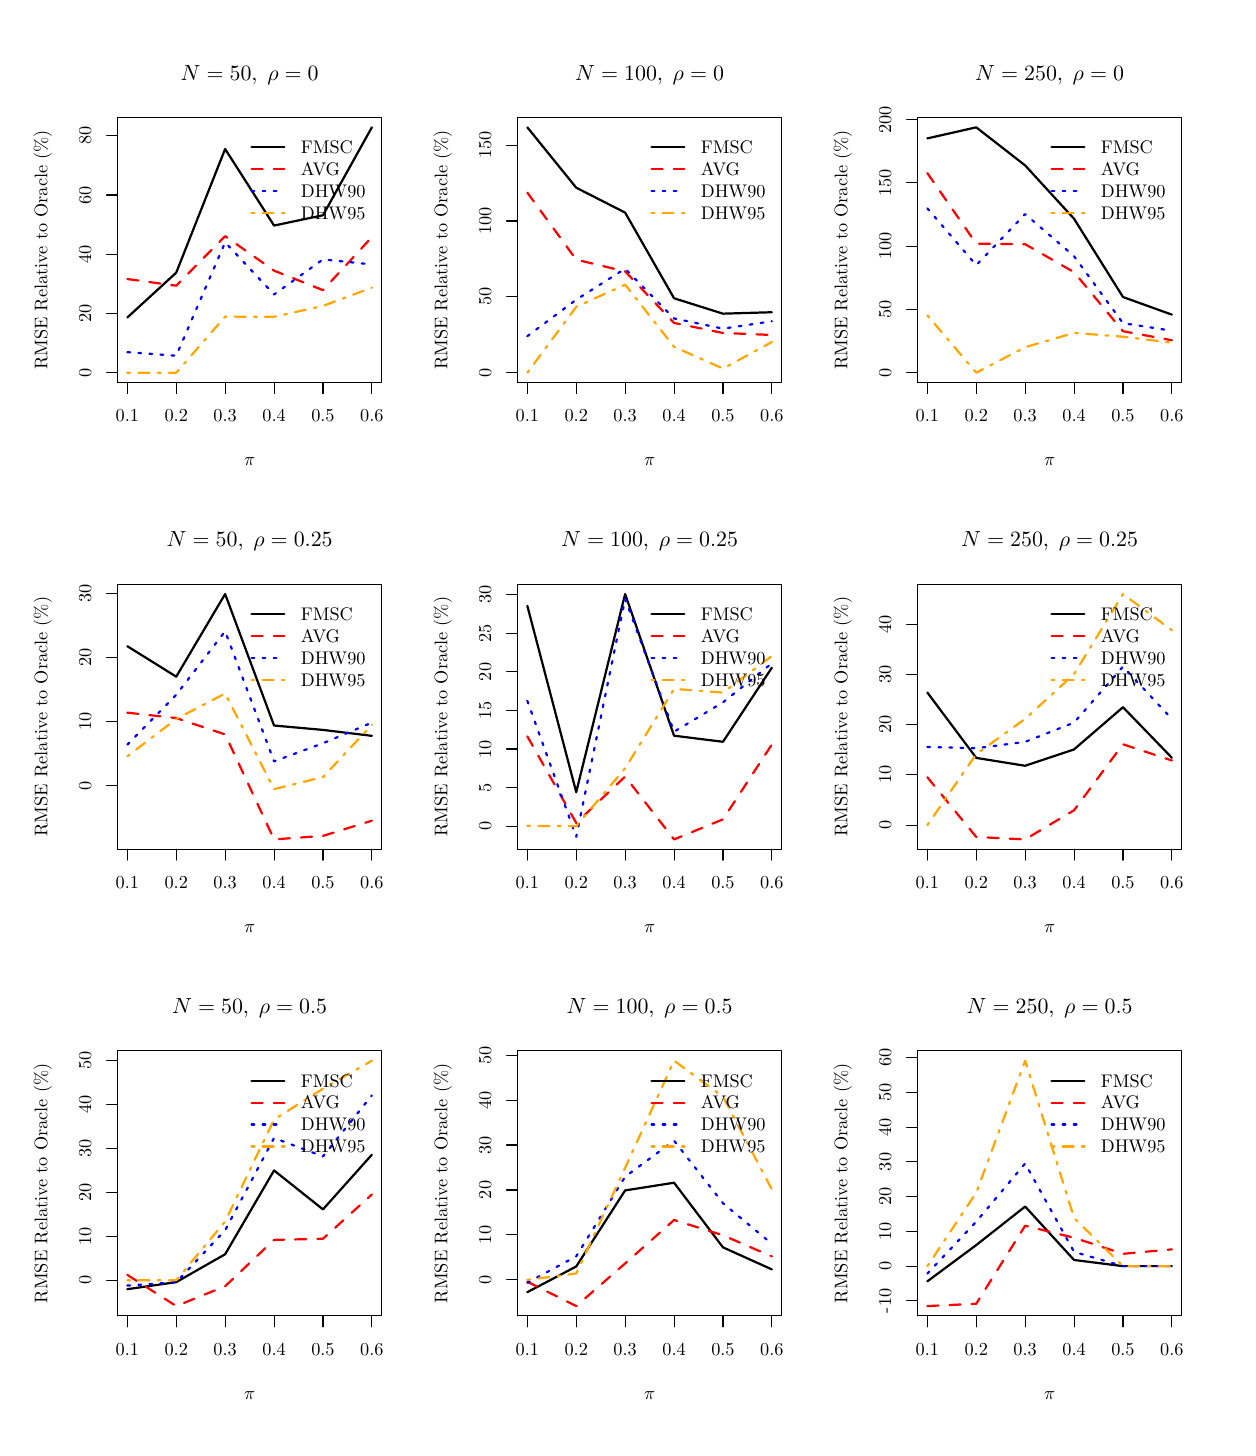
\begin{tikzpicture}[x=1pt,y=1pt]
\definecolor[named]{fillColor}{rgb}{1.00,1.00,1.00}
\path[use as bounding box,fill=fillColor,fill opacity=0.00] (0,0) rectangle (433.62,505.89);
\begin{scope}
\path[clip] ( 32.47,377.65) rectangle (127.91,473.42);
\definecolor[named]{drawColor}{rgb}{0.00,0.00,0.00}

\path[draw=drawColor,line width= 0.8pt,line join=round,line cap=round] ( 36.01,401.15) --
	( 53.68,417.36) --
	( 71.35,462.05) --
	( 89.03,434.38) --
	(106.70,438.10) --
	(124.37,469.87);
\end{scope}
\begin{scope}
\path[clip] (  0.00,  0.00) rectangle (433.62,505.89);
\definecolor[named]{drawColor}{rgb}{0.00,0.00,0.00}

\path[draw=drawColor,line width= 0.4pt,line join=round,line cap=round] ( 36.01,377.65) -- (124.37,377.65);

\path[draw=drawColor,line width= 0.4pt,line join=round,line cap=round] ( 36.01,377.65) -- ( 36.01,373.69);

\path[draw=drawColor,line width= 0.4pt,line join=round,line cap=round] ( 53.68,377.65) -- ( 53.68,373.69);

\path[draw=drawColor,line width= 0.4pt,line join=round,line cap=round] ( 71.35,377.65) -- ( 71.35,373.69);

\path[draw=drawColor,line width= 0.4pt,line join=round,line cap=round] ( 89.03,377.65) -- ( 89.03,373.69);

\path[draw=drawColor,line width= 0.4pt,line join=round,line cap=round] (106.70,377.65) -- (106.70,373.69);

\path[draw=drawColor,line width= 0.4pt,line join=round,line cap=round] (124.37,377.65) -- (124.37,373.69);

\node[text=drawColor,anchor=base,inner sep=0pt, outer sep=0pt, scale=  0.66] at ( 36.01,363.40) {0.1};

\node[text=drawColor,anchor=base,inner sep=0pt, outer sep=0pt, scale=  0.66] at ( 53.68,363.40) {0.2};

\node[text=drawColor,anchor=base,inner sep=0pt, outer sep=0pt, scale=  0.66] at ( 71.35,363.40) {0.3};

\node[text=drawColor,anchor=base,inner sep=0pt, outer sep=0pt, scale=  0.66] at ( 89.03,363.40) {0.4};

\node[text=drawColor,anchor=base,inner sep=0pt, outer sep=0pt, scale=  0.66] at (106.70,363.40) {0.5};

\node[text=drawColor,anchor=base,inner sep=0pt, outer sep=0pt, scale=  0.66] at (124.37,363.40) {0.6};

\path[draw=drawColor,line width= 0.4pt,line join=round,line cap=round] ( 32.47,381.20) -- ( 32.47,466.82);

\path[draw=drawColor,line width= 0.4pt,line join=round,line cap=round] ( 32.47,381.20) -- ( 28.51,381.20);

\path[draw=drawColor,line width= 0.4pt,line join=round,line cap=round] ( 32.47,402.61) -- ( 28.51,402.61);

\path[draw=drawColor,line width= 0.4pt,line join=round,line cap=round] ( 32.47,424.01) -- ( 28.51,424.01);

\path[draw=drawColor,line width= 0.4pt,line join=round,line cap=round] ( 32.47,445.42) -- ( 28.51,445.42);

\path[draw=drawColor,line width= 0.4pt,line join=round,line cap=round] ( 32.47,466.82) -- ( 28.51,466.82);

\node[text=drawColor,rotate= 90.00,anchor=base,inner sep=0pt, outer sep=0pt, scale=  0.66] at ( 22.97,381.20) {0};

\node[text=drawColor,rotate= 90.00,anchor=base,inner sep=0pt, outer sep=0pt, scale=  0.66] at ( 22.97,402.61) {20};

\node[text=drawColor,rotate= 90.00,anchor=base,inner sep=0pt, outer sep=0pt, scale=  0.66] at ( 22.97,424.01) {40};

\node[text=drawColor,rotate= 90.00,anchor=base,inner sep=0pt, outer sep=0pt, scale=  0.66] at ( 22.97,445.42) {60};

\node[text=drawColor,rotate= 90.00,anchor=base,inner sep=0pt, outer sep=0pt, scale=  0.66] at ( 22.97,466.82) {80};

\path[draw=drawColor,line width= 0.4pt,line join=round,line cap=round] ( 32.47,377.65) --
	(127.91,377.65) --
	(127.91,473.42) --
	( 32.47,473.42) --
	( 32.47,377.65);
\end{scope}
\begin{scope}
\path[clip] (  0.00,337.26) rectangle (144.54,505.89);
\definecolor[named]{drawColor}{rgb}{0.00,0.00,0.00}

\node[text=drawColor,anchor=base,inner sep=0pt, outer sep=0pt, scale=  0.79] at ( 80.19,486.92) {\bfseries $N=50, \;\rho=0$};

\node[text=drawColor,anchor=base,inner sep=0pt, outer sep=0pt, scale=  0.66] at ( 80.19,347.56) {$\pi$};

\node[text=drawColor,rotate= 90.00,anchor=base,inner sep=0pt, outer sep=0pt, scale=  0.66] at (  7.13,425.53) {RMSE Relative to Oracle (\%)};
\end{scope}
\begin{scope}
\path[clip] ( 32.47,377.65) rectangle (127.91,473.42);
\definecolor[named]{drawColor}{rgb}{1.00,0.00,0.00}

\path[draw=drawColor,line width= 0.8pt,dash pattern=on 4pt off 4pt ,line join=round,line cap=round] ( 36.01,415.06) --
	( 53.68,412.65) --
	( 71.35,430.56) --
	( 89.03,418.09) --
	(106.70,411.04) --
	(124.37,430.20);
\definecolor[named]{drawColor}{rgb}{0.00,0.00,1.00}

\path[draw=drawColor,line width= 0.8pt,dash pattern=on 1pt off 3pt ,line join=round,line cap=round] ( 36.01,388.64) --
	( 53.68,387.34) --
	( 71.35,428.32) --
	( 89.03,409.47) --
	(106.70,422.15) --
	(124.37,420.33);
\definecolor[named]{drawColor}{rgb}{1.00,0.65,0.00}

\path[draw=drawColor,line width= 0.8pt,dash pattern=on 1pt off 3pt on 4pt off 3pt ,line join=round,line cap=round] ( 36.01,381.20) --
	( 53.68,381.20) --
	( 71.35,401.48) --
	( 89.03,401.42) --
	(106.70,405.34) --
	(124.37,411.94);
\definecolor[named]{drawColor}{rgb}{0.00,0.00,0.00}

\path[draw=drawColor,line width= 0.8pt,line join=round,line cap=round] ( 80.89,462.63) -- ( 92.77,462.63);
\definecolor[named]{drawColor}{rgb}{1.00,0.00,0.00}

\path[draw=drawColor,line width= 0.8pt,dash pattern=on 4pt off 4pt ,line join=round,line cap=round] ( 80.89,454.71) -- ( 92.77,454.71);
\definecolor[named]{drawColor}{rgb}{0.00,0.00,1.00}

\path[draw=drawColor,line width= 0.8pt,dash pattern=on 1pt off 3pt ,line join=round,line cap=round] ( 80.89,446.79) -- ( 92.77,446.79);
\definecolor[named]{drawColor}{rgb}{1.00,0.65,0.00}

\path[draw=drawColor,line width= 0.8pt,dash pattern=on 1pt off 3pt on 4pt off 3pt ,line join=round,line cap=round] ( 80.89,438.87) -- ( 92.77,438.87);
\definecolor[named]{drawColor}{rgb}{0.00,0.00,0.00}

\node[text=drawColor,anchor=base west,inner sep=0pt, outer sep=0pt, scale=  0.66] at ( 98.71,460.35) {FMSC};

\node[text=drawColor,anchor=base west,inner sep=0pt, outer sep=0pt, scale=  0.66] at ( 98.71,452.43) {AVG};

\node[text=drawColor,anchor=base west,inner sep=0pt, outer sep=0pt, scale=  0.66] at ( 98.71,444.51) {DHW90};

\node[text=drawColor,anchor=base west,inner sep=0pt, outer sep=0pt, scale=  0.66] at ( 98.71,436.59) {DHW95};
\end{scope}
\begin{scope}
\path[clip] (177.01,377.65) rectangle (272.45,473.42);
\definecolor[named]{drawColor}{rgb}{0.00,0.00,0.00}

\path[draw=drawColor,line width= 0.8pt,line join=round,line cap=round] (180.55,469.87) --
	(198.22,448.06) --
	(215.89,439.06) --
	(233.57,408.10) --
	(251.24,402.54) --
	(268.91,403.06);
\end{scope}
\begin{scope}
\path[clip] (  0.00,  0.00) rectangle (433.62,505.89);
\definecolor[named]{drawColor}{rgb}{0.00,0.00,0.00}

\path[draw=drawColor,line width= 0.4pt,line join=round,line cap=round] (180.55,377.65) -- (268.91,377.65);

\path[draw=drawColor,line width= 0.4pt,line join=round,line cap=round] (180.55,377.65) -- (180.55,373.69);

\path[draw=drawColor,line width= 0.4pt,line join=round,line cap=round] (198.22,377.65) -- (198.22,373.69);

\path[draw=drawColor,line width= 0.4pt,line join=round,line cap=round] (215.89,377.65) -- (215.89,373.69);

\path[draw=drawColor,line width= 0.4pt,line join=round,line cap=round] (233.57,377.65) -- (233.57,373.69);

\path[draw=drawColor,line width= 0.4pt,line join=round,line cap=round] (251.24,377.65) -- (251.24,373.69);

\path[draw=drawColor,line width= 0.4pt,line join=round,line cap=round] (268.91,377.65) -- (268.91,373.69);

\node[text=drawColor,anchor=base,inner sep=0pt, outer sep=0pt, scale=  0.66] at (180.55,363.40) {0.1};

\node[text=drawColor,anchor=base,inner sep=0pt, outer sep=0pt, scale=  0.66] at (198.22,363.40) {0.2};

\node[text=drawColor,anchor=base,inner sep=0pt, outer sep=0pt, scale=  0.66] at (215.89,363.40) {0.3};

\node[text=drawColor,anchor=base,inner sep=0pt, outer sep=0pt, scale=  0.66] at (233.57,363.40) {0.4};

\node[text=drawColor,anchor=base,inner sep=0pt, outer sep=0pt, scale=  0.66] at (251.24,363.40) {0.5};

\node[text=drawColor,anchor=base,inner sep=0pt, outer sep=0pt, scale=  0.66] at (268.91,363.40) {0.6};

\path[draw=drawColor,line width= 0.4pt,line join=round,line cap=round] (177.01,381.20) -- (177.01,463.45);

\path[draw=drawColor,line width= 0.4pt,line join=round,line cap=round] (177.01,381.20) -- (173.05,381.20);

\path[draw=drawColor,line width= 0.4pt,line join=round,line cap=round] (177.01,408.62) -- (173.05,408.62);

\path[draw=drawColor,line width= 0.4pt,line join=round,line cap=round] (177.01,436.03) -- (173.05,436.03);

\path[draw=drawColor,line width= 0.4pt,line join=round,line cap=round] (177.01,463.45) -- (173.05,463.45);

\node[text=drawColor,rotate= 90.00,anchor=base,inner sep=0pt, outer sep=0pt, scale=  0.66] at (167.51,381.20) {0};

\node[text=drawColor,rotate= 90.00,anchor=base,inner sep=0pt, outer sep=0pt, scale=  0.66] at (167.51,408.62) {50};

\node[text=drawColor,rotate= 90.00,anchor=base,inner sep=0pt, outer sep=0pt, scale=  0.66] at (167.51,436.03) {100};

\node[text=drawColor,rotate= 90.00,anchor=base,inner sep=0pt, outer sep=0pt, scale=  0.66] at (167.51,463.45) {150};

\path[draw=drawColor,line width= 0.4pt,line join=round,line cap=round] (177.01,377.65) --
	(272.45,377.65) --
	(272.45,473.42) --
	(177.01,473.42) --
	(177.01,377.65);
\end{scope}
\begin{scope}
\path[clip] (144.54,337.26) rectangle (289.08,505.89);
\definecolor[named]{drawColor}{rgb}{0.00,0.00,0.00}

\node[text=drawColor,anchor=base,inner sep=0pt, outer sep=0pt, scale=  0.79] at (224.73,486.92) {\bfseries $N=100, \;\rho=0$};

\node[text=drawColor,anchor=base,inner sep=0pt, outer sep=0pt, scale=  0.66] at (224.73,347.56) {$\pi$};

\node[text=drawColor,rotate= 90.00,anchor=base,inner sep=0pt, outer sep=0pt, scale=  0.66] at (151.67,425.53) {RMSE Relative to Oracle (\%)};
\end{scope}
\begin{scope}
\path[clip] (177.01,377.65) rectangle (272.45,473.42);
\definecolor[named]{drawColor}{rgb}{1.00,0.00,0.00}

\path[draw=drawColor,line width= 0.8pt,dash pattern=on 4pt off 4pt ,line join=round,line cap=round] (180.55,446.28) --
	(198.22,422.06) --
	(215.89,417.81) --
	(233.57,399.19) --
	(251.24,395.57) --
	(268.91,394.84);
\definecolor[named]{drawColor}{rgb}{0.00,0.00,1.00}

\path[draw=drawColor,line width= 0.8pt,dash pattern=on 1pt off 3pt ,line join=round,line cap=round] (180.55,394.41) --
	(198.22,407.60) --
	(215.89,418.80) --
	(233.57,400.82) --
	(251.24,397.12) --
	(268.91,399.80);
\definecolor[named]{drawColor}{rgb}{1.00,0.65,0.00}

\path[draw=drawColor,line width= 0.8pt,dash pattern=on 1pt off 3pt on 4pt off 3pt ,line join=round,line cap=round] (180.55,381.20) --
	(198.22,405.02) --
	(215.89,413.03) --
	(233.57,390.56) --
	(251.24,382.69) --
	(268.91,392.30);
\definecolor[named]{drawColor}{rgb}{0.00,0.00,0.00}

\path[draw=drawColor,line width= 0.8pt,line join=round,line cap=round] (225.43,462.63) -- (237.31,462.63);
\definecolor[named]{drawColor}{rgb}{1.00,0.00,0.00}

\path[draw=drawColor,line width= 0.8pt,dash pattern=on 4pt off 4pt ,line join=round,line cap=round] (225.43,454.71) -- (237.31,454.71);
\definecolor[named]{drawColor}{rgb}{0.00,0.00,1.00}

\path[draw=drawColor,line width= 0.8pt,dash pattern=on 1pt off 3pt ,line join=round,line cap=round] (225.43,446.79) -- (237.31,446.79);
\definecolor[named]{drawColor}{rgb}{1.00,0.65,0.00}

\path[draw=drawColor,line width= 0.8pt,dash pattern=on 1pt off 3pt on 4pt off 3pt ,line join=round,line cap=round] (225.43,438.87) -- (237.31,438.87);
\definecolor[named]{drawColor}{rgb}{0.00,0.00,0.00}

\node[text=drawColor,anchor=base west,inner sep=0pt, outer sep=0pt, scale=  0.66] at (243.25,460.35) {FMSC};

\node[text=drawColor,anchor=base west,inner sep=0pt, outer sep=0pt, scale=  0.66] at (243.25,452.43) {AVG};

\node[text=drawColor,anchor=base west,inner sep=0pt, outer sep=0pt, scale=  0.66] at (243.25,444.51) {DHW90};

\node[text=drawColor,anchor=base west,inner sep=0pt, outer sep=0pt, scale=  0.66] at (243.25,436.59) {DHW95};
\end{scope}
\begin{scope}
\path[clip] (321.55,377.65) rectangle (416.99,473.42);
\definecolor[named]{drawColor}{rgb}{0.00,0.00,0.00}

\path[draw=drawColor,line width= 0.8pt,line join=round,line cap=round] (325.09,465.87) --
	(342.76,469.87) --
	(360.43,456.11) --
	(378.11,436.82) --
	(395.78,408.56) --
	(413.45,402.19);
\end{scope}
\begin{scope}
\path[clip] (  0.00,  0.00) rectangle (433.62,505.89);
\definecolor[named]{drawColor}{rgb}{0.00,0.00,0.00}

\path[draw=drawColor,line width= 0.4pt,line join=round,line cap=round] (325.09,377.65) -- (413.45,377.65);

\path[draw=drawColor,line width= 0.4pt,line join=round,line cap=round] (325.09,377.65) -- (325.09,373.69);

\path[draw=drawColor,line width= 0.4pt,line join=round,line cap=round] (342.76,377.65) -- (342.76,373.69);

\path[draw=drawColor,line width= 0.4pt,line join=round,line cap=round] (360.43,377.65) -- (360.43,373.69);

\path[draw=drawColor,line width= 0.4pt,line join=round,line cap=round] (378.11,377.65) -- (378.11,373.69);

\path[draw=drawColor,line width= 0.4pt,line join=round,line cap=round] (395.78,377.65) -- (395.78,373.69);

\path[draw=drawColor,line width= 0.4pt,line join=round,line cap=round] (413.45,377.65) -- (413.45,373.69);

\node[text=drawColor,anchor=base,inner sep=0pt, outer sep=0pt, scale=  0.66] at (325.09,363.40) {0.1};

\node[text=drawColor,anchor=base,inner sep=0pt, outer sep=0pt, scale=  0.66] at (342.76,363.40) {0.2};

\node[text=drawColor,anchor=base,inner sep=0pt, outer sep=0pt, scale=  0.66] at (360.43,363.40) {0.3};

\node[text=drawColor,anchor=base,inner sep=0pt, outer sep=0pt, scale=  0.66] at (378.11,363.40) {0.4};

\node[text=drawColor,anchor=base,inner sep=0pt, outer sep=0pt, scale=  0.66] at (395.78,363.40) {0.5};

\node[text=drawColor,anchor=base,inner sep=0pt, outer sep=0pt, scale=  0.66] at (413.45,363.40) {0.6};

\path[draw=drawColor,line width= 0.4pt,line join=round,line cap=round] (321.55,381.20) -- (321.55,472.67);

\path[draw=drawColor,line width= 0.4pt,line join=round,line cap=round] (321.55,381.20) -- (317.59,381.20);

\path[draw=drawColor,line width= 0.4pt,line join=round,line cap=round] (321.55,404.07) -- (317.59,404.07);

\path[draw=drawColor,line width= 0.4pt,line join=round,line cap=round] (321.55,426.94) -- (317.59,426.94);

\path[draw=drawColor,line width= 0.4pt,line join=round,line cap=round] (321.55,449.80) -- (317.59,449.80);

\path[draw=drawColor,line width= 0.4pt,line join=round,line cap=round] (321.55,472.67) -- (317.59,472.67);

\node[text=drawColor,rotate= 90.00,anchor=base,inner sep=0pt, outer sep=0pt, scale=  0.66] at (312.05,381.20) {0};

\node[text=drawColor,rotate= 90.00,anchor=base,inner sep=0pt, outer sep=0pt, scale=  0.66] at (312.05,404.07) {50};

\node[text=drawColor,rotate= 90.00,anchor=base,inner sep=0pt, outer sep=0pt, scale=  0.66] at (312.05,426.94) {100};

\node[text=drawColor,rotate= 90.00,anchor=base,inner sep=0pt, outer sep=0pt, scale=  0.66] at (312.05,449.80) {150};

\node[text=drawColor,rotate= 90.00,anchor=base,inner sep=0pt, outer sep=0pt, scale=  0.66] at (312.05,472.67) {200};

\path[draw=drawColor,line width= 0.4pt,line join=round,line cap=round] (321.55,377.65) --
	(416.99,377.65) --
	(416.99,473.42) --
	(321.55,473.42) --
	(321.55,377.65);
\end{scope}
\begin{scope}
\path[clip] (289.08,337.26) rectangle (433.62,505.89);
\definecolor[named]{drawColor}{rgb}{0.00,0.00,0.00}

\node[text=drawColor,anchor=base,inner sep=0pt, outer sep=0pt, scale=  0.79] at (369.27,486.92) {\bfseries $N=250, \;\rho=0$};

\node[text=drawColor,anchor=base,inner sep=0pt, outer sep=0pt, scale=  0.66] at (369.27,347.56) {$\pi$};

\node[text=drawColor,rotate= 90.00,anchor=base,inner sep=0pt, outer sep=0pt, scale=  0.66] at (296.21,425.53) {RMSE Relative to Oracle (\%)};
\end{scope}
\begin{scope}
\path[clip] (321.55,377.65) rectangle (416.99,473.42);
\definecolor[named]{drawColor}{rgb}{1.00,0.00,0.00}

\path[draw=drawColor,line width= 0.8pt,dash pattern=on 4pt off 4pt ,line join=round,line cap=round] (325.09,453.34) --
	(342.76,427.84) --
	(360.43,427.65) --
	(378.11,417.53) --
	(395.78,396.20) --
	(413.45,392.93);
\definecolor[named]{drawColor}{rgb}{0.00,0.00,1.00}

\path[draw=drawColor,line width= 0.8pt,dash pattern=on 1pt off 3pt ,line join=round,line cap=round] (325.09,440.61) --
	(342.76,420.05) --
	(360.43,438.52) --
	(378.11,423.30) --
	(395.78,399.11) --
	(413.45,396.38);
\definecolor[named]{drawColor}{rgb}{1.00,0.65,0.00}

\path[draw=drawColor,line width= 0.8pt,dash pattern=on 1pt off 3pt on 4pt off 3pt ,line join=round,line cap=round] (325.09,401.95) --
	(342.76,381.20) --
	(360.43,390.42) --
	(378.11,395.59) --
	(395.78,394.21) --
	(413.45,392.07);
\definecolor[named]{drawColor}{rgb}{0.00,0.00,0.00}

\path[draw=drawColor,line width= 0.8pt,line join=round,line cap=round] (369.97,462.63) -- (381.85,462.63);
\definecolor[named]{drawColor}{rgb}{1.00,0.00,0.00}

\path[draw=drawColor,line width= 0.8pt,dash pattern=on 4pt off 4pt ,line join=round,line cap=round] (369.97,454.71) -- (381.85,454.71);
\definecolor[named]{drawColor}{rgb}{0.00,0.00,1.00}

\path[draw=drawColor,line width= 0.8pt,dash pattern=on 1pt off 3pt ,line join=round,line cap=round] (369.97,446.79) -- (381.85,446.79);
\definecolor[named]{drawColor}{rgb}{1.00,0.65,0.00}

\path[draw=drawColor,line width= 0.8pt,dash pattern=on 1pt off 3pt on 4pt off 3pt ,line join=round,line cap=round] (369.97,438.87) -- (381.85,438.87);
\definecolor[named]{drawColor}{rgb}{0.00,0.00,0.00}

\node[text=drawColor,anchor=base west,inner sep=0pt, outer sep=0pt, scale=  0.66] at (387.79,460.35) {FMSC};

\node[text=drawColor,anchor=base west,inner sep=0pt, outer sep=0pt, scale=  0.66] at (387.79,452.43) {AVG};

\node[text=drawColor,anchor=base west,inner sep=0pt, outer sep=0pt, scale=  0.66] at (387.79,444.51) {DHW90};

\node[text=drawColor,anchor=base west,inner sep=0pt, outer sep=0pt, scale=  0.66] at (387.79,436.59) {DHW95};
\end{scope}
\begin{scope}
\path[clip] ( 32.47,209.02) rectangle (127.91,304.79);
\definecolor[named]{drawColor}{rgb}{0.00,0.00,0.00}

\path[draw=drawColor,line width= 0.8pt,line join=round,line cap=round] ( 36.01,282.38) --
	( 53.68,271.37) --
	( 71.35,301.24) --
	( 89.03,253.72) --
	(106.70,252.13) --
	(124.37,249.99);
\end{scope}
\begin{scope}
\path[clip] (  0.00,  0.00) rectangle (433.62,505.89);
\definecolor[named]{drawColor}{rgb}{0.00,0.00,0.00}

\path[draw=drawColor,line width= 0.4pt,line join=round,line cap=round] ( 36.01,209.02) -- (124.37,209.02);

\path[draw=drawColor,line width= 0.4pt,line join=round,line cap=round] ( 36.01,209.02) -- ( 36.01,205.06);

\path[draw=drawColor,line width= 0.4pt,line join=round,line cap=round] ( 53.68,209.02) -- ( 53.68,205.06);

\path[draw=drawColor,line width= 0.4pt,line join=round,line cap=round] ( 71.35,209.02) -- ( 71.35,205.06);

\path[draw=drawColor,line width= 0.4pt,line join=round,line cap=round] ( 89.03,209.02) -- ( 89.03,205.06);

\path[draw=drawColor,line width= 0.4pt,line join=round,line cap=round] (106.70,209.02) -- (106.70,205.06);

\path[draw=drawColor,line width= 0.4pt,line join=round,line cap=round] (124.37,209.02) -- (124.37,205.06);

\node[text=drawColor,anchor=base,inner sep=0pt, outer sep=0pt, scale=  0.66] at ( 36.01,194.77) {0.1};

\node[text=drawColor,anchor=base,inner sep=0pt, outer sep=0pt, scale=  0.66] at ( 53.68,194.77) {0.2};

\node[text=drawColor,anchor=base,inner sep=0pt, outer sep=0pt, scale=  0.66] at ( 71.35,194.77) {0.3};

\node[text=drawColor,anchor=base,inner sep=0pt, outer sep=0pt, scale=  0.66] at ( 89.03,194.77) {0.4};

\node[text=drawColor,anchor=base,inner sep=0pt, outer sep=0pt, scale=  0.66] at (106.70,194.77) {0.5};

\node[text=drawColor,anchor=base,inner sep=0pt, outer sep=0pt, scale=  0.66] at (124.37,194.77) {0.6};

\path[draw=drawColor,line width= 0.4pt,line join=round,line cap=round] ( 32.47,231.90) -- ( 32.47,301.58);

\path[draw=drawColor,line width= 0.4pt,line join=round,line cap=round] ( 32.47,231.90) -- ( 28.51,231.90);

\path[draw=drawColor,line width= 0.4pt,line join=round,line cap=round] ( 32.47,255.13) -- ( 28.51,255.13);

\path[draw=drawColor,line width= 0.4pt,line join=round,line cap=round] ( 32.47,278.35) -- ( 28.51,278.35);

\path[draw=drawColor,line width= 0.4pt,line join=round,line cap=round] ( 32.47,301.58) -- ( 28.51,301.58);

\node[text=drawColor,rotate= 90.00,anchor=base,inner sep=0pt, outer sep=0pt, scale=  0.66] at ( 22.97,231.90) {0};

\node[text=drawColor,rotate= 90.00,anchor=base,inner sep=0pt, outer sep=0pt, scale=  0.66] at ( 22.97,255.13) {10};

\node[text=drawColor,rotate= 90.00,anchor=base,inner sep=0pt, outer sep=0pt, scale=  0.66] at ( 22.97,278.35) {20};

\node[text=drawColor,rotate= 90.00,anchor=base,inner sep=0pt, outer sep=0pt, scale=  0.66] at ( 22.97,301.58) {30};

\path[draw=drawColor,line width= 0.4pt,line join=round,line cap=round] ( 32.47,209.02) --
	(127.91,209.02) --
	(127.91,304.79) --
	( 32.47,304.79) --
	( 32.47,209.02);
\end{scope}
\begin{scope}
\path[clip] (  0.00,168.63) rectangle (144.54,337.26);
\definecolor[named]{drawColor}{rgb}{0.00,0.00,0.00}

\node[text=drawColor,anchor=base,inner sep=0pt, outer sep=0pt, scale=  0.79] at ( 80.19,318.29) {\bfseries $N=50, \;\rho=0.25$};

\node[text=drawColor,anchor=base,inner sep=0pt, outer sep=0pt, scale=  0.66] at ( 80.19,178.93) {$\pi$};

\node[text=drawColor,rotate= 90.00,anchor=base,inner sep=0pt, outer sep=0pt, scale=  0.66] at (  7.13,256.90) {RMSE Relative to Oracle (\%)};
\end{scope}
\begin{scope}
\path[clip] ( 32.47,209.02) rectangle (127.91,304.79);
\definecolor[named]{drawColor}{rgb}{1.00,0.00,0.00}

\path[draw=drawColor,line width= 0.8pt,dash pattern=on 4pt off 4pt ,line join=round,line cap=round] ( 36.01,258.36) --
	( 53.68,256.41) --
	( 71.35,250.51) --
	( 89.03,212.57) --
	(106.70,213.83) --
	(124.37,219.33);
\definecolor[named]{drawColor}{rgb}{0.00,0.00,1.00}

\path[draw=drawColor,line width= 0.8pt,dash pattern=on 1pt off 3pt ,line join=round,line cap=round] ( 36.01,246.81) --
	( 53.68,264.82) --
	( 71.35,287.77) --
	( 89.03,240.78) --
	(106.70,247.31) --
	(124.37,254.76);
\definecolor[named]{drawColor}{rgb}{1.00,0.65,0.00}

\path[draw=drawColor,line width= 0.8pt,dash pattern=on 1pt off 3pt on 4pt off 3pt ,line join=round,line cap=round] ( 36.01,242.60) --
	( 53.68,256.07) --
	( 71.35,265.30) --
	( 89.03,230.73) --
	(106.70,235.10) --
	(124.37,253.92);
\definecolor[named]{drawColor}{rgb}{0.00,0.00,0.00}

\path[draw=drawColor,line width= 0.8pt,line join=round,line cap=round] ( 80.89,294.00) -- ( 92.77,294.00);
\definecolor[named]{drawColor}{rgb}{1.00,0.00,0.00}

\path[draw=drawColor,line width= 0.8pt,dash pattern=on 4pt off 4pt ,line join=round,line cap=round] ( 80.89,286.08) -- ( 92.77,286.08);
\definecolor[named]{drawColor}{rgb}{0.00,0.00,1.00}

\path[draw=drawColor,line width= 0.8pt,dash pattern=on 1pt off 3pt ,line join=round,line cap=round] ( 80.89,278.16) -- ( 92.77,278.16);
\definecolor[named]{drawColor}{rgb}{1.00,0.65,0.00}

\path[draw=drawColor,line width= 0.8pt,dash pattern=on 1pt off 3pt on 4pt off 3pt ,line join=round,line cap=round] ( 80.89,270.24) -- ( 92.77,270.24);
\definecolor[named]{drawColor}{rgb}{0.00,0.00,0.00}

\node[text=drawColor,anchor=base west,inner sep=0pt, outer sep=0pt, scale=  0.66] at ( 98.71,291.72) {FMSC};

\node[text=drawColor,anchor=base west,inner sep=0pt, outer sep=0pt, scale=  0.66] at ( 98.71,283.80) {AVG};

\node[text=drawColor,anchor=base west,inner sep=0pt, outer sep=0pt, scale=  0.66] at ( 98.71,275.88) {DHW90};

\node[text=drawColor,anchor=base west,inner sep=0pt, outer sep=0pt, scale=  0.66] at ( 98.71,267.96) {DHW95};
\end{scope}
\begin{scope}
\path[clip] (177.01,209.02) rectangle (272.45,304.79);
\definecolor[named]{drawColor}{rgb}{0.00,0.00,0.00}

\path[draw=drawColor,line width= 0.8pt,line join=round,line cap=round] (180.55,296.96) --
	(198.22,229.64) --
	(215.89,301.24) --
	(233.57,250.04) --
	(251.24,247.84) --
	(268.91,274.62);
\end{scope}
\begin{scope}
\path[clip] (  0.00,  0.00) rectangle (433.62,505.89);
\definecolor[named]{drawColor}{rgb}{0.00,0.00,0.00}

\path[draw=drawColor,line width= 0.4pt,line join=round,line cap=round] (180.55,209.02) -- (268.91,209.02);

\path[draw=drawColor,line width= 0.4pt,line join=round,line cap=round] (180.55,209.02) -- (180.55,205.06);

\path[draw=drawColor,line width= 0.4pt,line join=round,line cap=round] (198.22,209.02) -- (198.22,205.06);

\path[draw=drawColor,line width= 0.4pt,line join=round,line cap=round] (215.89,209.02) -- (215.89,205.06);

\path[draw=drawColor,line width= 0.4pt,line join=round,line cap=round] (233.57,209.02) -- (233.57,205.06);

\path[draw=drawColor,line width= 0.4pt,line join=round,line cap=round] (251.24,209.02) -- (251.24,205.06);

\path[draw=drawColor,line width= 0.4pt,line join=round,line cap=round] (268.91,209.02) -- (268.91,205.06);

\node[text=drawColor,anchor=base,inner sep=0pt, outer sep=0pt, scale=  0.66] at (180.55,194.77) {0.1};

\node[text=drawColor,anchor=base,inner sep=0pt, outer sep=0pt, scale=  0.66] at (198.22,194.77) {0.2};

\node[text=drawColor,anchor=base,inner sep=0pt, outer sep=0pt, scale=  0.66] at (215.89,194.77) {0.3};

\node[text=drawColor,anchor=base,inner sep=0pt, outer sep=0pt, scale=  0.66] at (233.57,194.77) {0.4};

\node[text=drawColor,anchor=base,inner sep=0pt, outer sep=0pt, scale=  0.66] at (251.24,194.77) {0.5};

\node[text=drawColor,anchor=base,inner sep=0pt, outer sep=0pt, scale=  0.66] at (268.91,194.77) {0.6};

\path[draw=drawColor,line width= 0.4pt,line join=round,line cap=round] (177.01,217.34) -- (177.01,300.98);

\path[draw=drawColor,line width= 0.4pt,line join=round,line cap=round] (177.01,217.34) -- (173.05,217.34);

\path[draw=drawColor,line width= 0.4pt,line join=round,line cap=round] (177.01,231.28) -- (173.05,231.28);

\path[draw=drawColor,line width= 0.4pt,line join=round,line cap=round] (177.01,245.22) -- (173.05,245.22);

\path[draw=drawColor,line width= 0.4pt,line join=round,line cap=round] (177.01,259.16) -- (173.05,259.16);

\path[draw=drawColor,line width= 0.4pt,line join=round,line cap=round] (177.01,273.10) -- (173.05,273.10);

\path[draw=drawColor,line width= 0.4pt,line join=round,line cap=round] (177.01,287.04) -- (173.05,287.04);

\path[draw=drawColor,line width= 0.4pt,line join=round,line cap=round] (177.01,300.98) -- (173.05,300.98);

\node[text=drawColor,rotate= 90.00,anchor=base,inner sep=0pt, outer sep=0pt, scale=  0.66] at (167.51,217.34) {0};

\node[text=drawColor,rotate= 90.00,anchor=base,inner sep=0pt, outer sep=0pt, scale=  0.66] at (167.51,231.28) {5};

\node[text=drawColor,rotate= 90.00,anchor=base,inner sep=0pt, outer sep=0pt, scale=  0.66] at (167.51,245.22) {10};

\node[text=drawColor,rotate= 90.00,anchor=base,inner sep=0pt, outer sep=0pt, scale=  0.66] at (167.51,259.16) {15};

\node[text=drawColor,rotate= 90.00,anchor=base,inner sep=0pt, outer sep=0pt, scale=  0.66] at (167.51,273.10) {20};

\node[text=drawColor,rotate= 90.00,anchor=base,inner sep=0pt, outer sep=0pt, scale=  0.66] at (167.51,287.04) {25};

\node[text=drawColor,rotate= 90.00,anchor=base,inner sep=0pt, outer sep=0pt, scale=  0.66] at (167.51,300.98) {30};

\path[draw=drawColor,line width= 0.4pt,line join=round,line cap=round] (177.01,209.02) --
	(272.45,209.02) --
	(272.45,304.79) --
	(177.01,304.79) --
	(177.01,209.02);
\end{scope}
\begin{scope}
\path[clip] (144.54,168.63) rectangle (289.08,337.26);
\definecolor[named]{drawColor}{rgb}{0.00,0.00,0.00}

\node[text=drawColor,anchor=base,inner sep=0pt, outer sep=0pt, scale=  0.79] at (224.73,318.29) {\bfseries $N=100, \;\rho=0.25$};

\node[text=drawColor,anchor=base,inner sep=0pt, outer sep=0pt, scale=  0.66] at (224.73,178.93) {$\pi$};

\node[text=drawColor,rotate= 90.00,anchor=base,inner sep=0pt, outer sep=0pt, scale=  0.66] at (151.67,256.90) {RMSE Relative to Oracle (\%)};
\end{scope}
\begin{scope}
\path[clip] (177.01,209.02) rectangle (272.45,304.79);
\definecolor[named]{drawColor}{rgb}{1.00,0.00,0.00}

\path[draw=drawColor,line width= 0.8pt,dash pattern=on 4pt off 4pt ,line join=round,line cap=round] (180.55,249.81) --
	(198.22,218.53) --
	(215.89,235.27) --
	(233.57,212.57) --
	(251.24,219.81) --
	(268.91,246.87);
\definecolor[named]{drawColor}{rgb}{0.00,0.00,1.00}

\path[draw=drawColor,line width= 0.8pt,dash pattern=on 1pt off 3pt ,line join=round,line cap=round] (180.55,262.65) --
	(198.22,213.53) --
	(215.89,299.54) --
	(233.57,251.48) --
	(251.24,262.09) --
	(268.91,276.21);
\definecolor[named]{drawColor}{rgb}{1.00,0.65,0.00}

\path[draw=drawColor,line width= 0.8pt,dash pattern=on 1pt off 3pt on 4pt off 3pt ,line join=round,line cap=round] (180.55,217.48) --
	(198.22,217.35) --
	(215.89,238.28) --
	(233.57,266.96) --
	(251.24,265.63) --
	(268.91,278.85);
\definecolor[named]{drawColor}{rgb}{0.00,0.00,0.00}

\path[draw=drawColor,line width= 0.8pt,line join=round,line cap=round] (225.43,294.00) -- (237.31,294.00);
\definecolor[named]{drawColor}{rgb}{1.00,0.00,0.00}

\path[draw=drawColor,line width= 0.8pt,dash pattern=on 4pt off 4pt ,line join=round,line cap=round] (225.43,286.08) -- (237.31,286.08);
\definecolor[named]{drawColor}{rgb}{0.00,0.00,1.00}

\path[draw=drawColor,line width= 0.8pt,dash pattern=on 1pt off 3pt ,line join=round,line cap=round] (225.43,278.16) -- (237.31,278.16);
\definecolor[named]{drawColor}{rgb}{1.00,0.65,0.00}

\path[draw=drawColor,line width= 0.8pt,dash pattern=on 1pt off 3pt on 4pt off 3pt ,line join=round,line cap=round] (225.43,270.24) -- (237.31,270.24);
\definecolor[named]{drawColor}{rgb}{0.00,0.00,0.00}

\node[text=drawColor,anchor=base west,inner sep=0pt, outer sep=0pt, scale=  0.66] at (243.25,291.72) {FMSC};

\node[text=drawColor,anchor=base west,inner sep=0pt, outer sep=0pt, scale=  0.66] at (243.25,283.80) {AVG};

\node[text=drawColor,anchor=base west,inner sep=0pt, outer sep=0pt, scale=  0.66] at (243.25,275.88) {DHW90};

\node[text=drawColor,anchor=base west,inner sep=0pt, outer sep=0pt, scale=  0.66] at (243.25,267.96) {DHW95};
\end{scope}
\begin{scope}
\path[clip] (321.55,209.02) rectangle (416.99,304.79);
\definecolor[named]{drawColor}{rgb}{0.00,0.00,0.00}

\path[draw=drawColor,line width= 0.8pt,line join=round,line cap=round] (325.09,265.65) --
	(342.76,242.02) --
	(360.43,239.17) --
	(378.11,245.09) --
	(395.78,260.33) --
	(413.45,242.07);
\end{scope}
\begin{scope}
\path[clip] (  0.00,  0.00) rectangle (433.62,505.89);
\definecolor[named]{drawColor}{rgb}{0.00,0.00,0.00}

\path[draw=drawColor,line width= 0.4pt,line join=round,line cap=round] (325.09,209.02) -- (413.45,209.02);

\path[draw=drawColor,line width= 0.4pt,line join=round,line cap=round] (325.09,209.02) -- (325.09,205.06);

\path[draw=drawColor,line width= 0.4pt,line join=round,line cap=round] (342.76,209.02) -- (342.76,205.06);

\path[draw=drawColor,line width= 0.4pt,line join=round,line cap=round] (360.43,209.02) -- (360.43,205.06);

\path[draw=drawColor,line width= 0.4pt,line join=round,line cap=round] (378.11,209.02) -- (378.11,205.06);

\path[draw=drawColor,line width= 0.4pt,line join=round,line cap=round] (395.78,209.02) -- (395.78,205.06);

\path[draw=drawColor,line width= 0.4pt,line join=round,line cap=round] (413.45,209.02) -- (413.45,205.06);

\node[text=drawColor,anchor=base,inner sep=0pt, outer sep=0pt, scale=  0.66] at (325.09,194.77) {0.1};

\node[text=drawColor,anchor=base,inner sep=0pt, outer sep=0pt, scale=  0.66] at (342.76,194.77) {0.2};

\node[text=drawColor,anchor=base,inner sep=0pt, outer sep=0pt, scale=  0.66] at (360.43,194.77) {0.3};

\node[text=drawColor,anchor=base,inner sep=0pt, outer sep=0pt, scale=  0.66] at (378.11,194.77) {0.4};

\node[text=drawColor,anchor=base,inner sep=0pt, outer sep=0pt, scale=  0.66] at (395.78,194.77) {0.5};

\node[text=drawColor,anchor=base,inner sep=0pt, outer sep=0pt, scale=  0.66] at (413.45,194.77) {0.6};

\path[draw=drawColor,line width= 0.4pt,line join=round,line cap=round] (321.55,217.74) -- (321.55,290.37);

\path[draw=drawColor,line width= 0.4pt,line join=round,line cap=round] (321.55,217.74) -- (317.59,217.74);

\path[draw=drawColor,line width= 0.4pt,line join=round,line cap=round] (321.55,235.90) -- (317.59,235.90);

\path[draw=drawColor,line width= 0.4pt,line join=round,line cap=round] (321.55,254.06) -- (317.59,254.06);

\path[draw=drawColor,line width= 0.4pt,line join=round,line cap=round] (321.55,272.21) -- (317.59,272.21);

\path[draw=drawColor,line width= 0.4pt,line join=round,line cap=round] (321.55,290.37) -- (317.59,290.37);

\node[text=drawColor,rotate= 90.00,anchor=base,inner sep=0pt, outer sep=0pt, scale=  0.66] at (312.05,217.74) {0};

\node[text=drawColor,rotate= 90.00,anchor=base,inner sep=0pt, outer sep=0pt, scale=  0.66] at (312.05,235.90) {10};

\node[text=drawColor,rotate= 90.00,anchor=base,inner sep=0pt, outer sep=0pt, scale=  0.66] at (312.05,254.06) {20};

\node[text=drawColor,rotate= 90.00,anchor=base,inner sep=0pt, outer sep=0pt, scale=  0.66] at (312.05,272.21) {30};

\node[text=drawColor,rotate= 90.00,anchor=base,inner sep=0pt, outer sep=0pt, scale=  0.66] at (312.05,290.37) {40};

\path[draw=drawColor,line width= 0.4pt,line join=round,line cap=round] (321.55,209.02) --
	(416.99,209.02) --
	(416.99,304.79) --
	(321.55,304.79) --
	(321.55,209.02);
\end{scope}
\begin{scope}
\path[clip] (289.08,168.63) rectangle (433.62,337.26);
\definecolor[named]{drawColor}{rgb}{0.00,0.00,0.00}

\node[text=drawColor,anchor=base,inner sep=0pt, outer sep=0pt, scale=  0.79] at (369.27,318.29) {\bfseries $N=250, \;\rho=0.25$};

\node[text=drawColor,anchor=base,inner sep=0pt, outer sep=0pt, scale=  0.66] at (369.27,178.93) {$\pi$};

\node[text=drawColor,rotate= 90.00,anchor=base,inner sep=0pt, outer sep=0pt, scale=  0.66] at (296.21,256.90) {RMSE Relative to Oracle (\%)};
\end{scope}
\begin{scope}
\path[clip] (321.55,209.02) rectangle (416.99,304.79);
\definecolor[named]{drawColor}{rgb}{1.00,0.00,0.00}

\path[draw=drawColor,line width= 0.8pt,dash pattern=on 4pt off 4pt ,line join=round,line cap=round] (325.09,235.04) --
	(342.76,213.45) --
	(360.43,212.57) --
	(378.11,223.11) --
	(395.78,246.94) --
	(413.45,241.09);
\definecolor[named]{drawColor}{rgb}{0.00,0.00,1.00}

\path[draw=drawColor,line width= 0.8pt,dash pattern=on 1pt off 3pt ,line join=round,line cap=round] (325.09,245.98) --
	(342.76,245.50) --
	(360.43,247.81) --
	(378.11,254.77) --
	(395.78,275.00) --
	(413.45,256.10);
\definecolor[named]{drawColor}{rgb}{1.00,0.65,0.00}

\path[draw=drawColor,line width= 0.8pt,dash pattern=on 1pt off 3pt on 4pt off 3pt ,line join=round,line cap=round] (325.09,217.74) --
	(342.76,243.38) --
	(360.43,256.13) --
	(378.11,272.27) --
	(395.78,301.24) --
	(413.45,288.16);
\definecolor[named]{drawColor}{rgb}{0.00,0.00,0.00}

\path[draw=drawColor,line width= 0.8pt,line join=round,line cap=round] (369.97,294.00) -- (381.85,294.00);
\definecolor[named]{drawColor}{rgb}{1.00,0.00,0.00}

\path[draw=drawColor,line width= 0.8pt,dash pattern=on 4pt off 4pt ,line join=round,line cap=round] (369.97,286.08) -- (381.85,286.08);
\definecolor[named]{drawColor}{rgb}{0.00,0.00,1.00}

\path[draw=drawColor,line width= 0.8pt,dash pattern=on 1pt off 3pt ,line join=round,line cap=round] (369.97,278.16) -- (381.85,278.16);
\definecolor[named]{drawColor}{rgb}{1.00,0.65,0.00}

\path[draw=drawColor,line width= 0.8pt,dash pattern=on 1pt off 3pt on 4pt off 3pt ,line join=round,line cap=round] (369.97,270.24) -- (381.85,270.24);
\definecolor[named]{drawColor}{rgb}{0.00,0.00,0.00}

\node[text=drawColor,anchor=base west,inner sep=0pt, outer sep=0pt, scale=  0.66] at (387.79,291.72) {FMSC};

\node[text=drawColor,anchor=base west,inner sep=0pt, outer sep=0pt, scale=  0.66] at (387.79,283.80) {AVG};

\node[text=drawColor,anchor=base west,inner sep=0pt, outer sep=0pt, scale=  0.66] at (387.79,275.88) {DHW90};

\node[text=drawColor,anchor=base west,inner sep=0pt, outer sep=0pt, scale=  0.66] at (387.79,267.96) {DHW95};
\end{scope}
\begin{scope}
\path[clip] ( 32.47, 40.39) rectangle (127.91,136.16);
\definecolor[named]{drawColor}{rgb}{0.00,0.00,0.00}

\path[draw=drawColor,line width= 0.8pt,line join=round,line cap=round] ( 36.01, 50.04) --
	( 53.68, 52.59) --
	( 71.35, 62.66) --
	( 89.03, 92.96) --
	(106.70, 78.87) --
	(124.37, 98.63);
\end{scope}
\begin{scope}
\path[clip] (  0.00,  0.00) rectangle (433.62,505.89);
\definecolor[named]{drawColor}{rgb}{0.00,0.00,0.00}

\path[draw=drawColor,line width= 0.4pt,line join=round,line cap=round] ( 36.01, 40.39) -- (124.37, 40.39);

\path[draw=drawColor,line width= 0.4pt,line join=round,line cap=round] ( 36.01, 40.39) -- ( 36.01, 36.43);

\path[draw=drawColor,line width= 0.4pt,line join=round,line cap=round] ( 53.68, 40.39) -- ( 53.68, 36.43);

\path[draw=drawColor,line width= 0.4pt,line join=round,line cap=round] ( 71.35, 40.39) -- ( 71.35, 36.43);

\path[draw=drawColor,line width= 0.4pt,line join=round,line cap=round] ( 89.03, 40.39) -- ( 89.03, 36.43);

\path[draw=drawColor,line width= 0.4pt,line join=round,line cap=round] (106.70, 40.39) -- (106.70, 36.43);

\path[draw=drawColor,line width= 0.4pt,line join=round,line cap=round] (124.37, 40.39) -- (124.37, 36.43);

\node[text=drawColor,anchor=base,inner sep=0pt, outer sep=0pt, scale=  0.66] at ( 36.01, 26.14) {0.1};

\node[text=drawColor,anchor=base,inner sep=0pt, outer sep=0pt, scale=  0.66] at ( 53.68, 26.14) {0.2};

\node[text=drawColor,anchor=base,inner sep=0pt, outer sep=0pt, scale=  0.66] at ( 71.35, 26.14) {0.3};

\node[text=drawColor,anchor=base,inner sep=0pt, outer sep=0pt, scale=  0.66] at ( 89.03, 26.14) {0.4};

\node[text=drawColor,anchor=base,inner sep=0pt, outer sep=0pt, scale=  0.66] at (106.70, 26.14) {0.5};

\node[text=drawColor,anchor=base,inner sep=0pt, outer sep=0pt, scale=  0.66] at (124.37, 26.14) {0.6};

\path[draw=drawColor,line width= 0.4pt,line join=round,line cap=round] ( 32.47, 53.26) -- ( 32.47,132.65);

\path[draw=drawColor,line width= 0.4pt,line join=round,line cap=round] ( 32.47, 53.26) -- ( 28.51, 53.26);

\path[draw=drawColor,line width= 0.4pt,line join=round,line cap=round] ( 32.47, 69.14) -- ( 28.51, 69.14);

\path[draw=drawColor,line width= 0.4pt,line join=round,line cap=round] ( 32.47, 85.02) -- ( 28.51, 85.02);

\path[draw=drawColor,line width= 0.4pt,line join=round,line cap=round] ( 32.47,100.90) -- ( 28.51,100.90);

\path[draw=drawColor,line width= 0.4pt,line join=round,line cap=round] ( 32.47,116.77) -- ( 28.51,116.77);

\path[draw=drawColor,line width= 0.4pt,line join=round,line cap=round] ( 32.47,132.65) -- ( 28.51,132.65);

\node[text=drawColor,rotate= 90.00,anchor=base,inner sep=0pt, outer sep=0pt, scale=  0.66] at ( 22.97, 53.26) {0};

\node[text=drawColor,rotate= 90.00,anchor=base,inner sep=0pt, outer sep=0pt, scale=  0.66] at ( 22.97, 69.14) {10};

\node[text=drawColor,rotate= 90.00,anchor=base,inner sep=0pt, outer sep=0pt, scale=  0.66] at ( 22.97, 85.02) {20};

\node[text=drawColor,rotate= 90.00,anchor=base,inner sep=0pt, outer sep=0pt, scale=  0.66] at ( 22.97,100.90) {30};

\node[text=drawColor,rotate= 90.00,anchor=base,inner sep=0pt, outer sep=0pt, scale=  0.66] at ( 22.97,116.77) {40};

\node[text=drawColor,rotate= 90.00,anchor=base,inner sep=0pt, outer sep=0pt, scale=  0.66] at ( 22.97,132.65) {50};

\path[draw=drawColor,line width= 0.4pt,line join=round,line cap=round] ( 32.47, 40.39) --
	(127.91, 40.39) --
	(127.91,136.16) --
	( 32.47,136.16) --
	( 32.47, 40.39);
\end{scope}
\begin{scope}
\path[clip] (  0.00,  0.00) rectangle (144.54,168.63);
\definecolor[named]{drawColor}{rgb}{0.00,0.00,0.00}

\node[text=drawColor,anchor=base,inner sep=0pt, outer sep=0pt, scale=  0.79] at ( 80.19,149.66) {\bfseries $N=50, \;\rho=0.5$};

\node[text=drawColor,anchor=base,inner sep=0pt, outer sep=0pt, scale=  0.66] at ( 80.19, 10.30) {$\pi$};

\node[text=drawColor,rotate= 90.00,anchor=base,inner sep=0pt, outer sep=0pt, scale=  0.66] at (  7.13, 88.27) {RMSE Relative to Oracle (\%)};
\end{scope}
\begin{scope}
\path[clip] ( 32.47, 40.39) rectangle (127.91,136.16);
\definecolor[named]{drawColor}{rgb}{1.00,0.00,0.00}

\path[draw=drawColor,line width= 0.8pt,dash pattern=on 4pt off 4pt ,line join=round,line cap=round] ( 36.01, 55.21) --
	( 53.68, 43.94) --
	( 71.35, 51.11) --
	( 89.03, 67.85) --
	(106.70, 68.26) --
	(124.37, 84.26);
\definecolor[named]{drawColor}{rgb}{0.00,0.00,1.00}

\path[draw=drawColor,line width= 0.8pt,dash pattern=on 1pt off 3pt ,line join=round,line cap=round] ( 36.01, 51.35) --
	( 53.68, 52.54) --
	( 71.35, 71.33) --
	( 89.03,104.69) --
	(106.70, 98.03) --
	(124.37,120.07);
\definecolor[named]{drawColor}{rgb}{1.00,0.65,0.00}

\path[draw=drawColor,line width= 0.8pt,dash pattern=on 1pt off 3pt on 4pt off 3pt ,line join=round,line cap=round] ( 36.01, 53.26) --
	( 53.68, 53.26) --
	( 71.35, 74.51) --
	( 89.03,111.36) --
	(106.70,122.48) --
	(124.37,132.61);
\definecolor[named]{drawColor}{rgb}{0.00,0.00,0.00}

\path[draw=drawColor,line width= 0.8pt,line join=round,line cap=round] ( 80.89,125.37) -- ( 92.77,125.37);
\definecolor[named]{drawColor}{rgb}{1.00,0.00,0.00}

\path[draw=drawColor,line width= 0.8pt,dash pattern=on 4pt off 4pt ,line join=round,line cap=round] ( 80.89,117.45) -- ( 92.77,117.45);
\definecolor[named]{drawColor}{rgb}{0.00,0.00,1.00}

\path[draw=drawColor,line width= 0.8pt,dash pattern=on 1pt off 3pt ,line join=round,line cap=round] ( 80.89,109.53) -- ( 92.77,109.53);
\definecolor[named]{drawColor}{rgb}{1.00,0.65,0.00}

\path[draw=drawColor,line width= 0.8pt,dash pattern=on 1pt off 3pt on 4pt off 3pt ,line join=round,line cap=round] ( 80.89,101.61) -- ( 92.77,101.61);
\definecolor[named]{drawColor}{rgb}{0.00,0.00,0.00}

\node[text=drawColor,anchor=base west,inner sep=0pt, outer sep=0pt, scale=  0.66] at ( 98.71,123.09) {FMSC};

\node[text=drawColor,anchor=base west,inner sep=0pt, outer sep=0pt, scale=  0.66] at ( 98.71,115.17) {AVG};

\node[text=drawColor,anchor=base west,inner sep=0pt, outer sep=0pt, scale=  0.66] at ( 98.71,107.25) {DHW90};

\node[text=drawColor,anchor=base west,inner sep=0pt, outer sep=0pt, scale=  0.66] at ( 98.71, 99.33) {DHW95};
\end{scope}
\begin{scope}
\path[clip] (177.01, 40.39) rectangle (272.45,136.16);
\definecolor[named]{drawColor}{rgb}{0.00,0.00,0.00}

\path[draw=drawColor,line width= 0.8pt,line join=round,line cap=round] (180.55, 48.97) --
	(198.22, 58.25) --
	(215.89, 85.73) --
	(233.57, 88.51) --
	(251.24, 65.16) --
	(268.91, 57.19);
\end{scope}
\begin{scope}
\path[clip] (  0.00,  0.00) rectangle (433.62,505.89);
\definecolor[named]{drawColor}{rgb}{0.00,0.00,0.00}

\path[draw=drawColor,line width= 0.4pt,line join=round,line cap=round] (180.55, 40.39) -- (268.91, 40.39);

\path[draw=drawColor,line width= 0.4pt,line join=round,line cap=round] (180.55, 40.39) -- (180.55, 36.43);

\path[draw=drawColor,line width= 0.4pt,line join=round,line cap=round] (198.22, 40.39) -- (198.22, 36.43);

\path[draw=drawColor,line width= 0.4pt,line join=round,line cap=round] (215.89, 40.39) -- (215.89, 36.43);

\path[draw=drawColor,line width= 0.4pt,line join=round,line cap=round] (233.57, 40.39) -- (233.57, 36.43);

\path[draw=drawColor,line width= 0.4pt,line join=round,line cap=round] (251.24, 40.39) -- (251.24, 36.43);

\path[draw=drawColor,line width= 0.4pt,line join=round,line cap=round] (268.91, 40.39) -- (268.91, 36.43);

\node[text=drawColor,anchor=base,inner sep=0pt, outer sep=0pt, scale=  0.66] at (180.55, 26.14) {0.1};

\node[text=drawColor,anchor=base,inner sep=0pt, outer sep=0pt, scale=  0.66] at (198.22, 26.14) {0.2};

\node[text=drawColor,anchor=base,inner sep=0pt, outer sep=0pt, scale=  0.66] at (215.89, 26.14) {0.3};

\node[text=drawColor,anchor=base,inner sep=0pt, outer sep=0pt, scale=  0.66] at (233.57, 26.14) {0.4};

\node[text=drawColor,anchor=base,inner sep=0pt, outer sep=0pt, scale=  0.66] at (251.24, 26.14) {0.5};

\node[text=drawColor,anchor=base,inner sep=0pt, outer sep=0pt, scale=  0.66] at (268.91, 26.14) {0.6};

\path[draw=drawColor,line width= 0.4pt,line join=round,line cap=round] (177.01, 53.41) -- (177.01,134.62);

\path[draw=drawColor,line width= 0.4pt,line join=round,line cap=round] (177.01, 53.41) -- (173.05, 53.41);

\path[draw=drawColor,line width= 0.4pt,line join=round,line cap=round] (177.01, 69.66) -- (173.05, 69.66);

\path[draw=drawColor,line width= 0.4pt,line join=round,line cap=round] (177.01, 85.90) -- (173.05, 85.90);

\path[draw=drawColor,line width= 0.4pt,line join=round,line cap=round] (177.01,102.14) -- (173.05,102.14);

\path[draw=drawColor,line width= 0.4pt,line join=round,line cap=round] (177.01,118.38) -- (173.05,118.38);

\path[draw=drawColor,line width= 0.4pt,line join=round,line cap=round] (177.01,134.62) -- (173.05,134.62);

\node[text=drawColor,rotate= 90.00,anchor=base,inner sep=0pt, outer sep=0pt, scale=  0.66] at (167.51, 53.41) {0};

\node[text=drawColor,rotate= 90.00,anchor=base,inner sep=0pt, outer sep=0pt, scale=  0.66] at (167.51, 69.66) {10};

\node[text=drawColor,rotate= 90.00,anchor=base,inner sep=0pt, outer sep=0pt, scale=  0.66] at (167.51, 85.90) {20};

\node[text=drawColor,rotate= 90.00,anchor=base,inner sep=0pt, outer sep=0pt, scale=  0.66] at (167.51,102.14) {30};

\node[text=drawColor,rotate= 90.00,anchor=base,inner sep=0pt, outer sep=0pt, scale=  0.66] at (167.51,118.38) {40};

\node[text=drawColor,rotate= 90.00,anchor=base,inner sep=0pt, outer sep=0pt, scale=  0.66] at (167.51,134.62) {50};

\path[draw=drawColor,line width= 0.4pt,line join=round,line cap=round] (177.01, 40.39) --
	(272.45, 40.39) --
	(272.45,136.16) --
	(177.01,136.16) --
	(177.01, 40.39);
\end{scope}
\begin{scope}
\path[clip] (144.54,  0.00) rectangle (289.08,168.63);
\definecolor[named]{drawColor}{rgb}{0.00,0.00,0.00}

\node[text=drawColor,anchor=base,inner sep=0pt, outer sep=0pt, scale=  0.79] at (224.73,149.66) {\bfseries $N=100, \;\rho=0.5$};

\node[text=drawColor,anchor=base,inner sep=0pt, outer sep=0pt, scale=  0.66] at (224.73, 10.30) {$\pi$};

\node[text=drawColor,rotate= 90.00,anchor=base,inner sep=0pt, outer sep=0pt, scale=  0.66] at (151.67, 88.27) {RMSE Relative to Oracle (\%)};
\end{scope}
\begin{scope}
\path[clip] (177.01, 40.39) rectangle (272.45,136.16);
\definecolor[named]{drawColor}{rgb}{1.00,0.00,0.00}

\path[draw=drawColor,line width= 0.8pt,dash pattern=on 4pt off 4pt ,line join=round,line cap=round] (180.55, 52.75) --
	(198.22, 43.94) --
	(215.89, 59.34) --
	(233.57, 75.04) --
	(251.24, 69.52) --
	(268.91, 61.86);
\definecolor[named]{drawColor}{rgb}{0.00,0.00,1.00}

\path[draw=drawColor,line width= 0.8pt,dash pattern=on 1pt off 3pt ,line join=round,line cap=round] (180.55, 52.35) --
	(198.22, 61.92) --
	(215.89, 90.70) --
	(233.57,103.70) --
	(251.24, 81.11) --
	(268.91, 66.43);
\definecolor[named]{drawColor}{rgb}{1.00,0.65,0.00}

\path[draw=drawColor,line width= 0.8pt,dash pattern=on 1pt off 3pt on 4pt off 3pt ,line join=round,line cap=round] (180.55, 53.41) --
	(198.22, 55.71) --
	(215.89, 93.91) --
	(233.57,132.61) --
	(251.24,119.62) --
	(268.91, 86.09);
\definecolor[named]{drawColor}{rgb}{0.00,0.00,0.00}

\path[draw=drawColor,line width= 0.8pt,line join=round,line cap=round] (225.43,125.37) -- (237.31,125.37);
\definecolor[named]{drawColor}{rgb}{1.00,0.00,0.00}

\path[draw=drawColor,line width= 0.8pt,dash pattern=on 4pt off 4pt ,line join=round,line cap=round] (225.43,117.45) -- (237.31,117.45);
\definecolor[named]{drawColor}{rgb}{0.00,0.00,1.00}

\path[draw=drawColor,line width= 0.8pt,dash pattern=on 1pt off 3pt ,line join=round,line cap=round] (225.43,109.53) -- (237.31,109.53);
\definecolor[named]{drawColor}{rgb}{1.00,0.65,0.00}

\path[draw=drawColor,line width= 0.8pt,dash pattern=on 1pt off 3pt on 4pt off 3pt ,line join=round,line cap=round] (225.43,101.61) -- (237.31,101.61);
\definecolor[named]{drawColor}{rgb}{0.00,0.00,0.00}

\node[text=drawColor,anchor=base west,inner sep=0pt, outer sep=0pt, scale=  0.66] at (243.25,123.09) {FMSC};

\node[text=drawColor,anchor=base west,inner sep=0pt, outer sep=0pt, scale=  0.66] at (243.25,115.17) {AVG};

\node[text=drawColor,anchor=base west,inner sep=0pt, outer sep=0pt, scale=  0.66] at (243.25,107.25) {DHW90};

\node[text=drawColor,anchor=base west,inner sep=0pt, outer sep=0pt, scale=  0.66] at (243.25, 99.33) {DHW95};
\end{scope}
\begin{scope}
\path[clip] (321.55, 40.39) rectangle (416.99,136.16);
\definecolor[named]{drawColor}{rgb}{0.00,0.00,0.00}

\path[draw=drawColor,line width= 0.8pt,line join=round,line cap=round] (325.09, 52.87) --
	(342.76, 65.98) --
	(360.43, 79.90) --
	(378.11, 60.60) --
	(395.78, 58.37) --
	(413.45, 58.37);
\end{scope}
\begin{scope}
\path[clip] (  0.00,  0.00) rectangle (433.62,505.89);
\definecolor[named]{drawColor}{rgb}{0.00,0.00,0.00}

\path[draw=drawColor,line width= 0.4pt,line join=round,line cap=round] (325.09, 40.39) -- (413.45, 40.39);

\path[draw=drawColor,line width= 0.4pt,line join=round,line cap=round] (325.09, 40.39) -- (325.09, 36.43);

\path[draw=drawColor,line width= 0.4pt,line join=round,line cap=round] (342.76, 40.39) -- (342.76, 36.43);

\path[draw=drawColor,line width= 0.4pt,line join=round,line cap=round] (360.43, 40.39) -- (360.43, 36.43);

\path[draw=drawColor,line width= 0.4pt,line join=round,line cap=round] (378.11, 40.39) -- (378.11, 36.43);

\path[draw=drawColor,line width= 0.4pt,line join=round,line cap=round] (395.78, 40.39) -- (395.78, 36.43);

\path[draw=drawColor,line width= 0.4pt,line join=round,line cap=round] (413.45, 40.39) -- (413.45, 36.43);

\node[text=drawColor,anchor=base,inner sep=0pt, outer sep=0pt, scale=  0.66] at (325.09, 26.14) {0.1};

\node[text=drawColor,anchor=base,inner sep=0pt, outer sep=0pt, scale=  0.66] at (342.76, 26.14) {0.2};

\node[text=drawColor,anchor=base,inner sep=0pt, outer sep=0pt, scale=  0.66] at (360.43, 26.14) {0.3};

\node[text=drawColor,anchor=base,inner sep=0pt, outer sep=0pt, scale=  0.66] at (378.11, 26.14) {0.4};

\node[text=drawColor,anchor=base,inner sep=0pt, outer sep=0pt, scale=  0.66] at (395.78, 26.14) {0.5};

\node[text=drawColor,anchor=base,inner sep=0pt, outer sep=0pt, scale=  0.66] at (413.45, 26.14) {0.6};

\path[draw=drawColor,line width= 0.4pt,line join=round,line cap=round] (321.55, 45.81) -- (321.55,133.67);

\path[draw=drawColor,line width= 0.4pt,line join=round,line cap=round] (321.55, 45.81) -- (317.59, 45.81);

\path[draw=drawColor,line width= 0.4pt,line join=round,line cap=round] (321.55, 58.37) -- (317.59, 58.37);

\path[draw=drawColor,line width= 0.4pt,line join=round,line cap=round] (321.55, 70.92) -- (317.59, 70.92);

\path[draw=drawColor,line width= 0.4pt,line join=round,line cap=round] (321.55, 83.47) -- (317.59, 83.47);

\path[draw=drawColor,line width= 0.4pt,line join=round,line cap=round] (321.55, 96.02) -- (317.59, 96.02);

\path[draw=drawColor,line width= 0.4pt,line join=round,line cap=round] (321.55,108.57) -- (317.59,108.57);

\path[draw=drawColor,line width= 0.4pt,line join=round,line cap=round] (321.55,121.12) -- (317.59,121.12);

\path[draw=drawColor,line width= 0.4pt,line join=round,line cap=round] (321.55,133.67) -- (317.59,133.67);

\node[text=drawColor,rotate= 90.00,anchor=base,inner sep=0pt, outer sep=0pt, scale=  0.66] at (312.05, 45.81) {-10};

\node[text=drawColor,rotate= 90.00,anchor=base,inner sep=0pt, outer sep=0pt, scale=  0.66] at (312.05, 58.37) {0};

\node[text=drawColor,rotate= 90.00,anchor=base,inner sep=0pt, outer sep=0pt, scale=  0.66] at (312.05, 70.92) {10};

\node[text=drawColor,rotate= 90.00,anchor=base,inner sep=0pt, outer sep=0pt, scale=  0.66] at (312.05, 83.47) {20};

\node[text=drawColor,rotate= 90.00,anchor=base,inner sep=0pt, outer sep=0pt, scale=  0.66] at (312.05, 96.02) {30};

\node[text=drawColor,rotate= 90.00,anchor=base,inner sep=0pt, outer sep=0pt, scale=  0.66] at (312.05,108.57) {40};

\node[text=drawColor,rotate= 90.00,anchor=base,inner sep=0pt, outer sep=0pt, scale=  0.66] at (312.05,121.12) {50};

\node[text=drawColor,rotate= 90.00,anchor=base,inner sep=0pt, outer sep=0pt, scale=  0.66] at (312.05,133.67) {60};

\path[draw=drawColor,line width= 0.4pt,line join=round,line cap=round] (321.55, 40.39) --
	(416.99, 40.39) --
	(416.99,136.16) --
	(321.55,136.16) --
	(321.55, 40.39);
\end{scope}
\begin{scope}
\path[clip] (289.08,  0.00) rectangle (433.62,168.63);
\definecolor[named]{drawColor}{rgb}{0.00,0.00,0.00}

\node[text=drawColor,anchor=base,inner sep=0pt, outer sep=0pt, scale=  0.79] at (369.27,149.66) {\bfseries $N=250, \;\rho=0.5$};

\node[text=drawColor,anchor=base,inner sep=0pt, outer sep=0pt, scale=  0.66] at (369.27, 10.30) {$\pi$};

\node[text=drawColor,rotate= 90.00,anchor=base,inner sep=0pt, outer sep=0pt, scale=  0.66] at (296.21, 88.27) {RMSE Relative to Oracle (\%)};
\end{scope}
\begin{scope}
\path[clip] (321.55, 40.39) rectangle (416.99,136.16);
\definecolor[named]{drawColor}{rgb}{1.00,0.00,0.00}

\path[draw=drawColor,line width= 0.8pt,dash pattern=on 4pt off 4pt ,line join=round,line cap=round] (325.09, 43.94) --
	(342.76, 44.77) --
	(360.43, 72.97) --
	(378.11, 68.63) --
	(395.78, 62.82) --
	(413.45, 64.44);
\definecolor[named]{drawColor}{rgb}{0.00,0.00,1.00}

\path[draw=drawColor,line width= 0.8pt,dash pattern=on 1pt off 3pt ,line join=round,line cap=round] (325.09, 55.67) --
	(342.76, 74.45) --
	(360.43, 95.46) --
	(378.11, 63.53) --
	(395.78, 58.37) --
	(413.45, 58.37);
\definecolor[named]{drawColor}{rgb}{1.00,0.65,0.00}

\path[draw=drawColor,line width= 0.8pt,dash pattern=on 1pt off 3pt on 4pt off 3pt ,line join=round,line cap=round] (325.09, 58.37) --
	(342.76, 84.89) --
	(360.43,132.61) --
	(378.11, 75.78) --
	(395.78, 58.37) --
	(413.45, 58.37);
\definecolor[named]{drawColor}{rgb}{0.00,0.00,0.00}

\path[draw=drawColor,line width= 0.8pt,line join=round,line cap=round] (369.97,125.37) -- (381.85,125.37);
\definecolor[named]{drawColor}{rgb}{1.00,0.00,0.00}

\path[draw=drawColor,line width= 0.8pt,dash pattern=on 4pt off 4pt ,line join=round,line cap=round] (369.97,117.45) -- (381.85,117.45);
\definecolor[named]{drawColor}{rgb}{0.00,0.00,1.00}

\path[draw=drawColor,line width= 0.8pt,dash pattern=on 1pt off 3pt ,line join=round,line cap=round] (369.97,109.53) -- (381.85,109.53);
\definecolor[named]{drawColor}{rgb}{1.00,0.65,0.00}

\path[draw=drawColor,line width= 0.8pt,dash pattern=on 1pt off 3pt on 4pt off 3pt ,line join=round,line cap=round] (369.97,101.61) -- (381.85,101.61);
\definecolor[named]{drawColor}{rgb}{0.00,0.00,0.00}

\node[text=drawColor,anchor=base west,inner sep=0pt, outer sep=0pt, scale=  0.66] at (387.79,123.09) {FMSC};

\node[text=drawColor,anchor=base west,inner sep=0pt, outer sep=0pt, scale=  0.66] at (387.79,115.17) {AVG};

\node[text=drawColor,anchor=base west,inner sep=0pt, outer sep=0pt, scale=  0.66] at (387.79,107.25) {DHW90};

\node[text=drawColor,anchor=base west,inner sep=0pt, outer sep=0pt, scale=  0.66] at (387.79, 99.33) {DHW95};
\end{scope}
\end{tikzpicture}

	\caption{Caption goes here.}
\end{figure}